\documentclass[a4paper]{report}
\usepackage[spanish]{babel}
\usepackage{graphicx}
\pagestyle{headings}
\titlepage
\usepackage[utf8]{inputenc} % para codificacion unicode (utf8)
\usepackage{enumerate}
\usepackage{hyperref} % para links a paginas web
\usepackage{subfig}
\usepackage{graphics}
\usepackage{amsmath}
\usepackage{amssymb}
\usepackage{amsthm}
\usepackage{placeins}
\usepackage{tabularx}
\usepackage{booktabs,siunitx}
\usepackage{calc}
\usepackage{bm}
\usepackage{fullpage}
\usepackage{mathdots}
\usepackage{multirow}

% plot a circle
\usepackage{tikz}
\newcommand\TikCircle[1][3]{\tikz[baseline=-#1]{\draw[thick](0,0.05)circle[radius=#1mm];}}


\decimalpoint

% That follow is for listings configuration
\usepackage{listings}
\usepackage{color}
\usepackage{textcomp}
\definecolor{listinggray}{gray}{0.9}
\definecolor{lbcolor}{rgb}{0.99,0.99,0.99}
\lstset{
    backgroundcolor=\color{lbcolor},
    tabsize=4,
    rulecolor=,
    language=python,
    basicstyle=\scriptsize,
    upquote=true,
    aboveskip={1.5\baselineskip},
    columns=fixed,
    showstringspaces=false,
    extendedchars=true,
    breaklines=true,
    prebreak = \raisebox{0ex}[0ex][0ex]{\ensuremath{\hookleftarrow}},
    frame=single,
    showtabs=false,
    showspaces=false,
    showstringspaces=false,
    identifierstyle=\ttfamily,
    keywordstyle=\color[rgb]{0,0,1},
    commentstyle=\color[rgb]{0.133,0.545,0.133},
    stringstyle=\color[rgb]{0.627,0.126,0.941},
    literate=%
        {á}{{\'{a}}}1
        {é}{{\'{e}}}1
        {í}{{\'{i}}}1
        {ó}{{\'{o}}}1
        {ú}{{\'{u}}}1
        {ñ}{{\~n}}1
}
\newcommand{\var}{\operatorname{var}}
\newcommand{\x}{\mathbf{x}}
\newcommand{\y}{\mathbf{y}}
\newcommand{\w}{\mathbf{w}}
\newcommand{\z}{\mathbf{z}}
\newcommand{\g}{\mathbf{g}}
\newcommand{\h}{\mathbf{h}}
\newcommand{\s}{\mathbf{s}}
\newcommand{\thetabf}{\bm{\theta}}
\newcommand{\alphabf}{\bm{\alpha}}
\newcommand{\mubf}{\bm{\mu}}
\newcommand{\I}{\mathbf{I}} % Fisher information matrix
\newcommand{\C}{\mathbf{C}} % Covariance matrix
\newcommand{\abf}{\mathbf{a}}
\newcommand{\bbf}{\mathbf{b}}
\newcommand{\e}{\mathbf{e}}
\newcommand{\ubf}{\mathbf{u}}
\newcommand{\vbf}{\mathbf{v}}
\newcommand{\A}{\mathbf{A}}
\newcommand{\B}{\mathbf{B}}
\newcommand{\D}{\mathbf{D}}
\newcommand{\G}{\mathbf{G}}
\newcommand{\Hbf}{\mathbf{H}}
\newcommand{\K}{\mathbf{K}}
\newcommand{\Lbf}{\mathbf{L}}
\newcommand{\M}{\mathbf{M}}
\newcommand{\R}{\mathbf{R}}
\newcommand{\T}{\mathbf{T}}
\newcommand{\W}{\mathbf{W}}
\newcommand{\X}{\mathbf{X}}
\newcommand{\Pbf}{\mathbf{P}}
\renewcommand{\Re}{\operatorname{Re}}
\renewcommand{\Im}{\operatorname{Im}}
\DeclareMathOperator*{\argmin}{arg\,min}
\DeclareMathOperator*{\argmax}{arg\,max}
\DeclareMathOperator{\tr}{tr}
\DeclareMathOperator{\cov}{cov}
\DeclareMathOperator{\Arg}{Arg}
\DeclareMathOperator{\Log}{Log}
\DeclareMathOperator{\sech}{sech}
\DeclareMathOperator{\csch}{csch}


\title{Estudiando el libro ``Complex variables and applications''\\de J. W. Brown y R. V. Churchill}
\author{Ernesto López}


\begin{document} 

\hypersetup{pageanchor=false}
\maketitle
\hypersetup{pageanchor=true}
\pagenumbering{roman}
\tableofcontents


\chapter*{Prefacio}

El presente documento consiste en apuntes sobre el libro ``Complex variables and applications'' \cite{brown2013complex}.

\pagenumbering{arabic}

\chapter{Números complejos}

\section{Algunas propiedades algebraicas}

La \emph{fórmula binomial} es válida para números complejos. Si \(z_1\) y \(z_2\) son dos números complejos distintos de cero, se cumple que\footnote{La prueba puede encontrarse en \url{https://en.wikipedia.org/wiki/Binomial_theorem}, por ejemplo.} 
\begin{equation}\label{eq:binomial_theorem}
 (z_1+z_2)^n=\sum_{k=0}^n\binom{n}{k}z_1^{k}z_2^{n-k}=\sum_{k=0}^n\binom{n}{k}z_1^{n-k}z_2^k,
 \qquad\qquad\textrm{con}\qquad\qquad
 n=1,\,2,\,\dots,
\end{equation}
donde
\[
 \binom{n}{k}=\frac{n!}{k!(n-k)!}.
\]

\section{Forma exponencial}\label{sec:exponential_form}

Sean \(r\) y \(\theta\) las coordenadas polares del punto \((x,\,y)\) que corresponden a un número complejo \(z=x+iy\) no nulo. Como \(x=r\cos\theta\) y \(y=r\sen\theta\) el número \(z\) puede escribirse en \emph{forma polar} como 
\[
 z=r(\cos\theta+i\sen\theta).
\]
Si \(z=0\), la coordenada \(\theta\) es indefinida, y por lo tanto se asume que \(z\neq0\) cuando se emplean coordenadas polares.

En análisis complejo, no se permite que el número real \(r\) sea negativo, y representa el largo del vector \(z\). El número real \(\theta\) representa el ángulo que forma el vector \(z\) con el eje real positivo medido en radianes. Como en cálculo, \(\theta\) tiene un conjunto infinito de valores posibles, incluyendo números negativos, que difieren en múltiplos enteros de \(2\pi\). Dichos valores pueden ser determinados por la ecuación \(\tan\theta=y/x\), donde debe especificarse el cuadrante que contiene al punto \(z\), como se explicará enseguida. Cada valor de \(\theta\) se llama \emph{argumento} de \(z\) y el conjunto de todos los valores se denota como \(\arg z\). El \emph{valor principal} de \(\arg z\), denotado como \(\Arg z\), es el único valor \(\Theta\) tal que \(-\pi<\Theta\leq\pi\). De esta forma,
\[
 \arg z=\Arg z+2n\pi,
 \qquad\qquad
 n=0,\,\pm1,\,\pm2,\,\dots.
\]
Cuando \(z\) es un número real negativo, \(\Arg z\) toma el valor \(\pi\) y no \(-\pi\).

Cuando un número complejo está representado por un argumento \(\arg z\) que no es el principal, al argumento principal \(\Arg z\) puede obtenerse como \cite{haber2019complex}
\begin{equation}\label{eq:principal_argument_from_argument}
 \Arg z=\arg z+2N_c\pi, 
\end{equation}
donde \(N_c\) es un número entero dado por 
\begin{equation}\label{eq:principal_argument_from_argument_Nc}
 N_c=\left\lfloor\frac{1}{2}-\frac{\arg z}{2\pi}\right\rfloor,
\end{equation}
y el operador \(\lfloor\cdot\rfloor\) denota el mayor entero, esto es, \(\lfloor x\rfloor\) es el mayor entero menor o igual a \(x\). Efectivamente, supóngase que se dispone de \(\arg z=\Theta+2N\pi\), donde \(\Theta\) es el argumento principal desconocido, con \(-\pi<\Theta\leq\pi\), y \(N\) cualquier número entero. De esta forma, de la ecuación \ref{eq:principal_argument_from_argument_Nc},
\[
 N_c=\left\lfloor\frac{1}{2}-\frac{\arg z}{2\pi}\right\rfloor
 =\left\lfloor\frac{1}{2}-\frac{\Theta+2N\pi}{2\pi}\right\rfloor
 =\left\lfloor\frac{1}{2}-\frac{\Theta}{2\pi}-N\right\rfloor
 =\left\lfloor\frac{\pi-\Theta}{2\pi}\right\rfloor-N
 =-N
\]
donde en la última igualdad se consideró que 
\[
 \textrm{como}\qquad
 -\pi<\Theta\leq\pi
 \qquad\textrm{se cumple que}\qquad 
 0\leq\pi-\Theta<2\pi
 \qquad\textrm{y por lo tanto}\qquad
 \left\lfloor\frac{\pi-\Theta}{2\pi}\right\rfloor=0.
\]
Sustituyendo el resultado \(N_c=-N\) en la ecuación \ref{eq:principal_argument_from_argument}, se tiene que 
\[
 \Arg z=\arg z+2N_c\pi=(\Theta+2N\pi)-2N\pi=\Theta,
\]
como se requiere.

Como consideración adicional respecto al argumento, se observa que la función tangente es periódica de período \(\pi\) con rango todos los números reales. Por lo tanto, dado un número real \(x\), la ecuación \(\tan\theta=x\) tiene infinitas soluciones. Si se considera como dominio únicamente un período, por ejemplo el intervalo \((-\pi/2,\,\pi/2)\), la función es uno a uno y por lo tanto invertible. La solución \(\theta=\tan^{-1}x\) en ese intervalo se llama valor principal de la ecuación \(\tan\theta=x\), y las infinitas soluciones son \(\theta=\tan^{-1}x+n\pi\) con \(n=0,\,\pm1,\,\pm2,\,\dots\). De esta forma, dado un número complejo \(z=x+iy\), la solución \(\tan^{-1}y/x\) es un ángulo en el intervalo \((-\pi/2,\,\pi/2)\), que corresponde a un complejo en el primer o cuarto cuadrante del plano. Esto significa que \(\tan^{-1}y/x\) brinda el argumento principal de \(z\) si \(z\) pertenece al primer o cuarto cuadrante. Puede deducirse que si el complejo \(z\) pertenece al segundo cuadrante, es decir, cumple que \(x<0\) y \(y\geq0\), el argumento principal se obtiene como \(\Arg z=\pi+\tan^{-1}y/x\) y si el complejo \(z\) pertenece al tercer cuadrante, es decir, cumple que \(x<0\) y \(y<0\), el argumento principal se obtiene como \(\Arg z=-\pi+\tan^{-1}y/x\).

\section{Productos y potencias en forma exponencial}\label{sec:exponential_form_products_and_powers}

Mediante trigonometría puede verse que \(e^{i\theta}\) tiene la propiedad aditiva familiar de la función exponencial en cálculo:
\[
 e^{i\theta_1}e^{i\theta_2}=e^{i(\theta_1+\theta_2)}.
\]
Por lo tanto, si \(z_1=r_1e^{i\theta_1}\) y \(z_2=r_2e^{i\theta_2}\), el producto \(z_1z_2\) tiene la forma exponencial
\[
 z_1z_2=(r_1r_2)e^{i(\theta_1+\theta_1)}.
\]
Además,
\[
 \frac{z_1}{z_2}=\frac{r_1}{r_2}e^{i(\theta_1-\theta_2)}.
\]
De esta expresión se deduce que el inverso de un número complejo \(re^{i\theta}\) no nulo es
\begin{equation}\label{eq:exponential_form_inverse}
  z^{-1}=\frac{1}{r}e^{-i\theta}.
\end{equation}
Otro resultado importante que puede obtenerse formalmente empleando reglas de los números reales es
\begin{equation}\label{eq:power_with_n_integer}
 z^n=r^ne^{in\theta},
 \qquad\qquad\textrm{con}\qquad\qquad
 n=0,\,\pm1,\pm2,\,\dots. 
\end{equation}
Finalmente, se observa que si \(r=1\), esta ecuación queda
\[
 (e^{i\theta})^n=e^{in\theta},
 \qquad\qquad\textrm{con}\qquad\qquad
 n=0,\,\pm1,\pm2,\,\dots,
\]
y escrita en forma rectangular
\[
 (\cos\theta+i\sen\theta)^n=\cos n\theta+i\sen n\theta,
 \qquad\qquad\textrm{con}\qquad\qquad
 n=0,\,\pm1,\pm2,\,\dots,
\]
se conoce como \emph{fórmula de de Moivre}.

\section{Argumento de productos y cocientes}\label{sec:argument_of_products}

Si \(z_1=r_1e^{i\theta_1}\) y \(z_2=r_2e^{i\theta_2}\), la expresión
\[
 z_1z_2=(r_1r_2)e^{i(\theta_1+\theta_1)}
\]
en la sección \ref{sec:exponential_form_products_and_powers} puede emplearse para obtener la importante identidad sobre argumentos
\begin{equation}\label{eq:argument_of_products}
 \arg(z_1z_2)=\arg(z_1)+\arg(z_2). 
\end{equation} 
La interpretación de la ecuación \ref{eq:argument_of_products} es la siguiente: si se especifican dos de los tres argumentos multivaluados en la ecuación, hay un valor del tercer argumento tal que la ecuación se cumple.

La ecuación \ref{eq:argument_of_products} es a veces válida si se reemplaza \(\arg\) por \(\Arg\). El siguiente ejemplo muestra que no siempre es el caso.

\paragraph{Ejemplo} Cuando \(z_1=-1\) y \(z_2=i\),
\[
 \Arg(z_1z_2)=\Arg(-i)=-\frac{\pi}{2}
 \qquad\qquad\textrm{pero}\qquad\qquad
 \Arg z_1+\Arg z_2=\pi+\frac{\pi}{2}=\frac{3\pi}{2}.
\]
Sin embargo, tomando estos mismos valores de \(\arg z_1\) y \(\arg z_2\) y eligiendo el valor 
\[
 \Arg(z_1z_2)+2\pi=-\frac{\pi}{2}+2\pi=\frac{3\pi}{2}.
\]
para \(\arg(z_1z_2)\), se observa que se cumple la ecuación \ref{eq:argument_of_products}.

De las ecuaciones \ref{eq:argument_of_products} y \ref{eq:exponential_form_inverse} puede deducirse que 
\begin{equation}\label{eq:argument_of_quotient}
 \arg\left(\frac{z_1}{z_2}\right)=\arg z_1-\arg z_2, 
\end{equation}
ecuación que se interpreta de la misma forma que la ecuación \ref{eq:argument_of_products}.

\section{Raíces de números complejos}

La expresión \(z^n=r^ne^{in\theta}\) de potencias enteras de números complejos dada por la ecuación \ref{eq:power_with_n_integer} es útil para encontrar las \(n\) raíces de un número complejo \(z_0=r_0e^{i\theta_0}\) no nulo, donde \(n\) tiene alguno de los valores \(n=2,\,3,\,\dots\). Considerando el hecho de que una raíz \(n\)-ésima de \(z_0\) es un número no nulo tal que \(z^n=z_0\), puede mostrarse que las \(n\) raíces distintas \(c_k\) de \(z_0\) son
\begin{equation}\label{eq:roots_n}
 c_k=\sqrt[n]{r_0}\exp\left(\frac{\theta_0}{n}+\frac{2k\pi}{n}\right),
 \qquad\qquad k=0,\,1,\,2,\,\dots,\,n-1. 
\end{equation}

Se empleará la notación \(z_0^{1/n}\) para indicar el conjunto completo de las \(n\) raíces de \(z_0\). Si \(z_0\) es un número real positivo \(r_0\), el símbolo \(r_0^{1/n}\) denota el conjunto completo de raíces y el símbolo \(\sqrt[n]{r_0}\) en la ecuación \ref{eq:roots_n} se reserva para la única raíz positiva. Cuando el valor de \(\theta_0\) empleado en la ecuación \ref{eq:roots_n} es el valor principal de \(\arg z_0\) (\(-\pi<\theta_0\leq\pi\)), el numero \(c_0\) es referido como \emph{raíz principal}. De esta forma, cuando \(z_0\) es un número real positivo, su raíz principal es \(\sqrt[n]{r_0}\).

\section{Regiones en el plano complejo}\label{sec:complex_plane_regions}

Esta sección trata sobre conjuntos de números complejos. El concepto mas básico es el de \emph{entorno} \(\epsilon\)
\[
 |z-z_0|<\epsilon
\]
de un punto \(z_0\), que consiste en todos los puntos \(z\) que se encuentran dentro de la circunferencia de radio \(\epsilon\) centrada en \(z_0\) pero no sobre ella. Ocasionalmente es necesario considerar el \emph{entorno reducido}
\[
 0<|z-z_0|<\epsilon,
\]
que es el entono \(\epsilon\) de \(z_0\) pero sin considerar el punto \(z_0\).

Se dice que un punto \(z_0\) es un \emph{punto interior} de un conjunto \(S\) si existe algún entorno de \(z_0\) que contiene solo puntos de \(S\) y se dice que \(z_0\) es un \emph{punto exterior} de \(S\) si existe un entorno de él que no contiene puntos de \(S\). Si \(z_0\) no cumple ninguna de estas condiciones se dice que es un \emph{punto de la frontera} de \(S\). Por lo tanto, un punto de la frontera es un punto cuyos entornos contienen al menos un punto de \(S\) y un punto que no es de \(S\). El conjunto de todos los puntos de la frontera se llama \emph{frontera} de \(S\). Por ejemplo, la circunferencia \(|z|=1\) es la frontera de cada un de los conjuntos
\begin{equation}\label{eq:open_and_closed_sets_example}
 |z|<1
 \qquad\qquad\textrm{y}\qquad\qquad
 |z|\leq1.
\end{equation}

Un conjunto es \emph{abierto} si no contiene ninguno de los puntos de su frontera. Se puede probar que un conjunto es abierto si y solo si todos sus puntos son interiores. Un conjunto es \emph{cerrado} si contiene todos los puntos de su frontera, y la \emph{clausura} de un conjunto \(S\) es el conjunto cerrado que consiste en todos los puntos de \(S\) y los de la frontera de \(S\). Observar que el primer conjunto en \ref{eq:open_and_closed_sets_example} es abierto y el segundo conjunto es su clausura.

Algunos conjuntos no son abiertos ni cerrados. Un conjunto \(S\) no es abierto si existe algún punto de su frontera contenido en él y un conjunto \(S\) no es cerrado si existe algún punto de la frontera no contenido en el. Por ejemplo, el disco perforado \(0<|z|<1\) no es un conjunto abierto ni cerrado. Por otro lado, el conjunto de todos los números complejos es abierto y cerrado ya que no tiene puntos de la frontera.  

Un conjunto \(S\) es \emph{acotado} si cada punto de \(S\) está dentro de algún círculo \(|z|\leq R\). En caso contrario es \emph{no acotado}. Ambos conjuntos en \ref{eq:open_and_closed_sets_example} son acotados, y la mitad del plano complejo \(\Re z\geq0\) es un conjunto no acotado.

\chapter{Funciones analíticas}

\section{Funciones y mapeos}

Sea \(S\) un conjunto de números complejos. Una función \(f\) es una regla que asigna a cada número complejo \(z\) en \(S\) un número complejo \(w\). El número \(w\) se llama \emph{valor} de \(f\) en \(z\) y se denota como \(f(z)\). De esta forma, \(w=f(z)\). El conjunto \(S\) se llama dominio de \(f\).

Supóngase que \(u+iv\) es el valor de la función en \(z=x+iy\), es decir,
\[
 u+iv=f(x+iy).
\]
Cada uno de los números reales \(u\) y \(v\) dependen de las variables reales \(x\) y \(y\), por lo que \(f(z)\) puede expresarse como dos funciones reales con variables reales \(x\) y \(y\), es decir,
\[
 f(z)=u(x,\,y)+iv(x,\,y).
\]
Si la función \(v\) es siempre nula, el valor de \(f(z)\) es real, y \(f\) es una función real de variable compleja.

Si se emplean las coordenadas polares \(r\) y \(\theta\) en lugar de \(x\) y \(y\), entonces
\[
 u+iv=f(re^{i\theta}),
\]
donde \(w=u+iv\) y \(z=re^{i\theta}\). En ese caso, se puede escribir
\[
 f(z)=u(r,\,\theta)+iv(r,\,\theta).
\]

A diferencia de las funciones reales con variable real, no hay una representación gráfica conveniente de una función compleja debido a que los números \(z\) y \(w\) se encuentran en un plano en lugar de una recta. Sin embargo, es posible exhibir información sobre la función indicando pares de correspondencia entre puntos \(z=(x,\,y)\) y \(w=(u,\,v)\). Cuando una función es pensada de esta forma, se suele llamar \emph{mapeo} o \emph{transformación}. La \emph{imagen} de un punto \(z\) en el dominio \(S\) es el punto \(w=f(z)\), y el conjunto de imágenes de todos los puntos de un conjunto \(T\) contenido en \(S\) se llama imagen de \(T\). La imagen del dominio completo \(S\) se llama \emph{rango} de \(f\). La \emph{imagen inversa} de un punto \(w\) es el conjunto de puntos \(z\) en el dominio de \(f\) que tienen a \(w\) como imagen. La imagen inversa de un punto puede ser un único punto, muchos puntos, o ninguno. El último caso ocurre cuando \(w\) no está en el rango de \(f\). Términos como \emph{traslación}, \emph{rotación} o \emph{reflexión} se emplean para describir las características de algunos mapeos.

\section{El mapeo \texorpdfstring{\(w=z^2\)}{w=z2}}\label{sec:square_mapping}

El mapeo \(w=z^2\) consiste en la transformación
\begin{equation}\label{eq:square_mapping}
  u=x^2-y^2,\qquad\qquad v=2xy
\end{equation}
del plano \(xy\) en el plano \(uv\). Este mapeo transforma ciertas hipérbolas del plano \(xy\) en rectas en el plano \(uv\), como se explicará a continuación.

Previamente, se recuerda que 
\begin{equation}\label{eq:hyperbola_canonical_equation}
 \frac{x^2}{a^2}-\frac{y^2}{b^2}=1 
\end{equation}
es la ecuación de una hipérbola\footnote{Ver \url{https://en.wikipedia.org/wiki/Hyperbola}, por ejemplo.} con 
\begin{itemize}
 \item eje mayor: la recta \(y=0\)
 \item centro: el origen de coordenadas
 \item vértices: \((\pm a,\,0)\)
 \item focos: \((\pm c,\,0)\), donde \(c^2=a^2+b^2\).
 \item asíntotas: las rectas \(y=\pm (b/a)x\).
\end{itemize}
En el caso en que \(a=b\) la hipérbola se dice \emph{rectangular} debido a que las asíntotas se intersectan formando ángulos rectos. Si los ejes de coordenadas se rotan un ángulo \(\theta\) en sentido horario formando el nuevo eje de coordenadas \(x'y'\), las coordenadas de un punto \((x,\,y)\) en función de las coordenadas en el nuevo eje son\footnote{Ver \url{https://en.wikipedia.org/wiki/Rotation_of_axes}, por ejemplo.}
\[
  x=x'\cos\theta-y'\sen\theta,\qquad\qquad
  y=-x'\sen\theta+y'\cos\theta.
\]
En particular, si el ángulo de rotación es \(\theta=-\pi/4\), que implica una rotación de \(\pi/4\) radianes en sentido horario como se muestra en la figura \ref{fig:square_mapping_rotated_hyperbola}, se cumple que
\[
 x=\frac{\sqrt{2}}{2}\left(x'+y'\right),\qquad\qquad
 y=\frac{\sqrt{2}}{2}\left(-x'+y'\right),
\]
por lo que en el nuevo eje de coordenadas, la ecuación de una hipérbola rectangular es
\[
 \frac{(x'+y')^2}{2a^2}+\frac{(-x'+y')^2}{2a^2}=1,
\]
que operando, se reduce a 
\begin{equation}\label{eq:rectangular_hyperbola_1st_3rd_quadrant_equation}
 \frac{2x'y'}{a^2}=1.
\end{equation}
\begin{figure}[!htb]
  \begin{minipage}[c]{0.45\textwidth}
    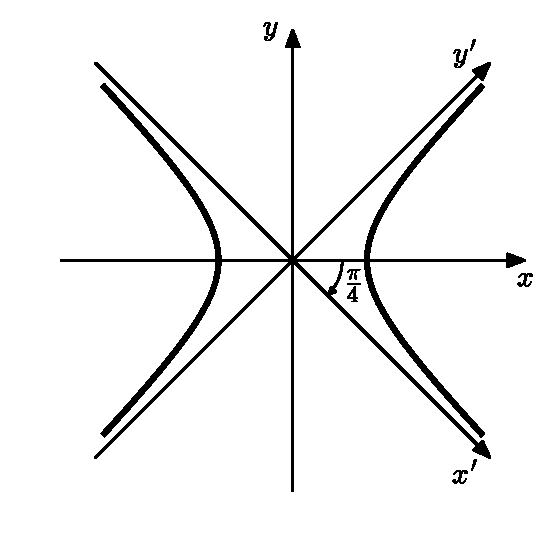
\includegraphics[width=\textwidth]{figuras/square_mapping_rotated_hyperbola.pdf}
  \end{minipage}\hfill
  \begin{minipage}[c]{0.45\textwidth}
    \caption{
       La rotación del eje de coordenadas \(xy\) de una hipérbola rectangular dada por la ecuación \ref{eq:hyperbola_canonical_equation} un ángulo de \(\pi/4\) radianes produce una hipérbola rectangular dada por la ecuación \ref{eq:rectangular_hyperbola_1st_3rd_quadrant_equation} contenida en el primer y tercer cuadrante en el nuevo eje de coordenadas \(x'y'\).
    } \label{fig:square_mapping_rotated_hyperbola}
  \end{minipage}
\end{figure}
Como se muestra en la figura \ref{fig:square_mapping_rotated_hyperbola}, esta es la ecuación de una hipérbola rectangular contenida en el primer y tercer cuadrante con 
\begin{itemize}
 \item eje mayor: la recta \(y=x\)
 \item centro: el origen de coordenadas
 \item vértices: \((\sqrt{a},\,\sqrt{a})\) y \((-\sqrt{a},\,-\sqrt{a})\)
 \item asíntotas: los ejes de coordenadas.
\end{itemize}

Retornando a la transformación \(w=z^2\) y teniendo en cuenta estas consideraciones, de la ecuación \ref{eq:square_mapping} se observa que cada rama de la hipérbola rectangular
\begin{equation}\label{eq:rectangular_hyperbola_horizontal}
 x^2-y^2=c_1\qquad\qquad\textrm{con}\qquad\qquad c_1>0,
\end{equation}
se mapea de forma uno a uno en la recta vertical \(u=c_1\). Efectivamente, la primera ecuación en \ref{eq:square_mapping} indica que \(u=c_1\) cuando \((x,\,y)\) es un punto de cualquier rama de la hipérbola. Además, los puntos con \(x=\sqrt{y^2+c_1}\) corresponden a la rama derecha y los puntos con \(x=-\sqrt{y^2+c_1}\) corresponden a la rama izquierda. Cuando por ejemplo un punto pertenece a la rama derecha, la segunda ecuación en \ref{eq:square_mapping} indica que \(v=2y\sqrt{y^2+c_1}\), y por lo tanto, la imagen de la rama derecha puede expresarse paramétricamente como
\[
 u=c_1,\qquad\qquad v=2y\sqrt{y^2+c_1}\qquad\qquad\textrm{con}\qquad\qquad-\infty<y<\infty.
\]
Esto muestra que la imagen de un punto \((x,\,y)\) en la rama derecha se mueve hacia arriba en la recta vertical a medida que \((x,\,y)\) se mueve hacia arriba en dicha rama. Análogamente, el par de ecuaciones
\[
 u=c_1,\qquad\qquad v=-2y\sqrt{y^2+c_1}\qquad\qquad\textrm{con}\qquad\qquad-\infty<y<\infty,
\]
es la representación paramétrica de la imagen de la rama izquierda de la hipérbola, y muestra que la imagen de un punto que se mueve hacia abajo por toda la rama izquierda es un punto que se mueve hacia arriba por toda la recta \(u=c_1\). Esto se ilustra en la figura \ref{fig:square_mapping_hyperbola}.
\begin{figure}[!htb]
 \begin{center}
 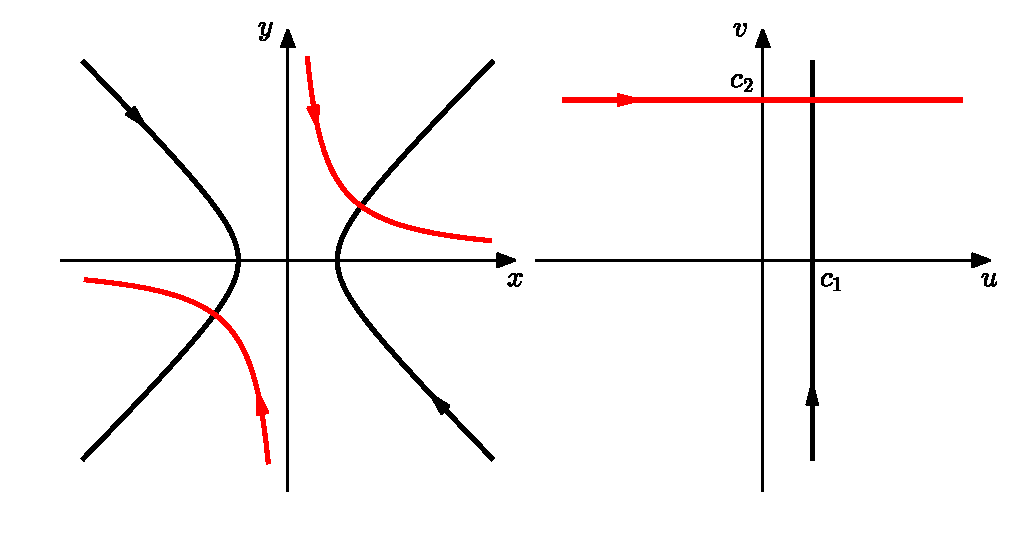
\includegraphics[width=0.85\textwidth]{figuras/square_mapping_hyperbola.pdf}
 \caption{\label{fig:square_mapping_hyperbola} Transformación \(w=z^2\). Las hipérbolas rectangulares \(x^2-y^2=c_1\) en el plano \(xy\) se mapean en rectas verticales \(u=c_1\) en el plano \(uv\) y las hipérbolas rectangulares \(2xy=c_2\) se mapean en rectas horizontales \(v=c_2\).}
 \end{center}
\end{figure}

Por otro lado, cada rama de la hipérbola 
\[
 2xy=c_2\qquad\qquad\textrm{con}\qquad\qquad c_2>0,
\]
se transforma en la recta \(v=c_2\). Para verificarlo, se observa de la segunda ecuación de \ref{eq:square_mapping} que \(v=c_2\) cuando \((x,\,y)\) es un punto de cualquiera de las ramas. Supóngase que el punto \((x,\,y)\) pertenece a la rama del primer cuadrante. Como \(y=c_2/(2x)\), la primera ecuación en \ref{eq:square_mapping} revela que la imagen de la rama tiene la representación paramétrica
\[
 u=x^2-\frac{c_2^2}{4x^2},\qquad\qquad v=c_2\qquad\qquad\textrm{con}\qquad\qquad0<x<\infty.
\]
Observando que 
\[
 \lim_{x\to0^+}u=-\infty
 \qquad\qquad\textrm{y}\qquad\qquad
 \lim_{x\to\infty}u=\infty,
\]
como \(u\) es continua en \(x\), es claro que a medida que \((x,\,y)\) se mueve hacia abajo en la rama del primer cuadrante, su imagen se mueve hacia la derecha sobre toda la recta \(v=c_2\). Además, la rama del tercer cuadrante tiene la representación paramétrica
\[
 u=\frac{c_2^2}{4y^2}-y^2,\qquad\qquad v=c_2\qquad\qquad\textrm{con}\qquad\qquad-\infty<y<0.
\]
Como
\[
 \lim_{y\to-\infty}u=-\infty
 \qquad\qquad\textrm{y}\qquad\qquad
 \lim_{y\to0^-}u=\infty,
\]
y \(u\) es continua en \(y\), se concluye que la imagen de un punto \((x,\,y)\) que se mueve hacia arriba en por toda la rama del tercer cuadrante se mueve hacia la derecha por toda la recta \(v=c_2\), como se muestra en la figura \ref{fig:square_mapping_hyperbola}.

\subsection*{Ejercicios}

A continuación se incluyen algunos ejercicios de la sección 14.

\subsubsection{Ejercicio 5}

Encontrar el dominio en el plano \(z\) cuya imagen bajo la transformación \(w=z^2\) es el dominio cuadrado en el plano \(w\) delimitado por las rectas \(u=1\), \(u=2\), \(v=1\) y \(v=2\).

\paragraph{Solución} Según lo discutido en la sección \ref{sec:square_mapping}, el mapeo \(w=z^2\) transforma la hipérbola \(x^2-y^2=c\) del plano \(z\) en la recta vertical \(u=c\) del plano \(w\) y la hipérbola \(2xy=c\) del plano \(z\) en la recta horizontal \(v=c\) del plano \(w\), como se muestra en la figura \ref{fig:square_mapping_hyperbola}. Por lo tanto, el cuadrado del plano \(w\) es la imagen de la región delimitada por las hipérbolas
\[
 x^2-y^2=1,\qquad x^2-y^2=2, \qquad 2xy=1\qquad\textrm{y}\qquad 2xy=2, 
\]
que se muestra en la figura \ref{fig:exercise_14_05}. 
\begin{figure}[!htb]
 \begin{center}
 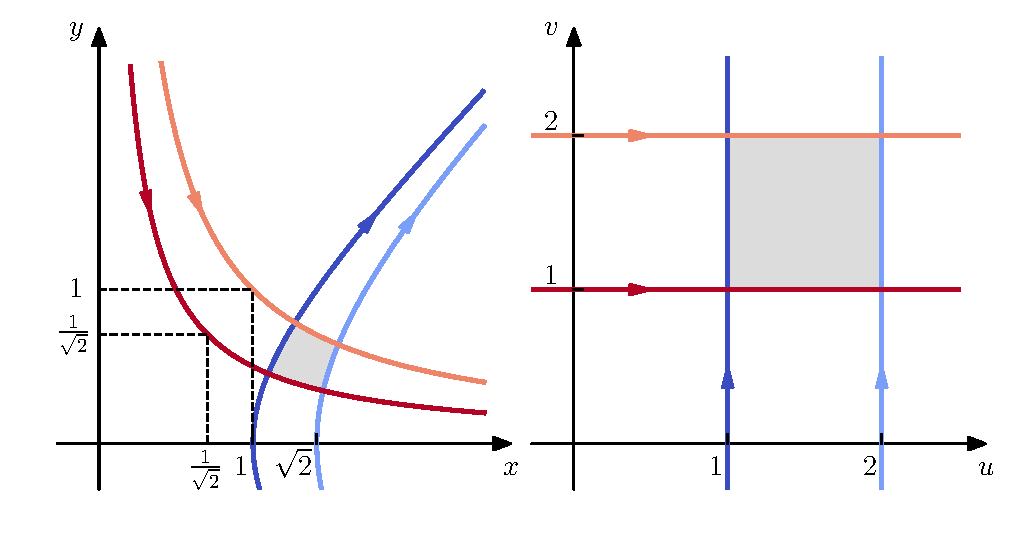
\includegraphics[width=0.85\textwidth]{figuras/exercise_14_05.pdf}
 \caption{\label{fig:exercise_14_05} Ejercicio 5. En la transformación \(w=z^2\) el cuadrado en el plano \(w\) es la imagen de la región delimitada por las hipérbolas en el plano \(z\).}
 \end{center}
\end{figure}

\subsubsection{Ejercicio 6}

Encontrar y graficar, mostrando las orientaciones correspondientes, las imágenes de las hipérbolas 
\[
 x^2-y^2=c_1,\qquad c_1<0\qquad\qquad\textrm{y}\qquad\qquad 2xy=c_2,\qquad c_2<0
\]
bajo la transformación \(w=z^2\).

\paragraph{Solución} Se parte observando que
\[
 x^2-y^2=c_1,\qquad c_1<0
\]
es una hipérbola rectangular con eje mayor la recta \(x=0\) y vértices en \((0,\,\pm\sqrt{-c_1})\), como se muestra en la figura \ref{fig:exercise_14_06}. Esto es porque su ecuación se puede escribir como \(y^2-x^2=c_1'\) donde \(c_1'=-c_1>0\), por lo que su gráfica es como la hipérbola de la ecuación \ref{eq:rectangular_hyperbola_horizontal} pero intercambiando los ejes de coordenadas. La primera ecuación en \ref{eq:square_mapping} indica que cada rama de la hipérbola se transforma en la recta vertical \(u=c_1\). En particular, los puntos con \(y=\sqrt{x^2-c_1}\) corresponden a la rama superior y los puntos con \(y=-\sqrt{x^2-c_1}\) corresponden a la rama inferior. Cuando un punto pertenece a la rama superior, la segunda ecuación en \ref{eq:square_mapping} indica que \(v=2x\sqrt{x^2-c_1}\), y por lo tanto, la imagen de la rama superior puede expresarse paramétricamente como
\[
 u=c_1,\qquad\qquad v=2x\sqrt{x^2-c_1}\qquad\qquad\textrm{con}\qquad\qquad-\infty<x<\infty.
\]
Esto muestra que la imagen de un punto \((x,\,y)\) en la rama superior se mueve hacia arriba en la recta vertical a medida que \((x,\,y)\) se mueve hacia la derecha en dicha rama. Análogamente, la representación paramétrica de un punto en la rama inferior es
\[
 u=c_1,\qquad\qquad v=-2x\sqrt{x^2-c_1}\qquad\qquad\textrm{con}\qquad\qquad-\infty<x<\infty
\]
y muestra que a medida que \(x\) crece, \(v\) decrece. Por lo tanto, un punto \((x,\,y)\) en la rama inferior que se mueve a la izquierda tiene como imagen un punto que se mueve hacia arriba en la recta vertical \(u=c_1\). Esto se ilustra en la figura \ref{fig:exercise_14_06}.
\begin{figure}[!htb]
 \begin{center}
 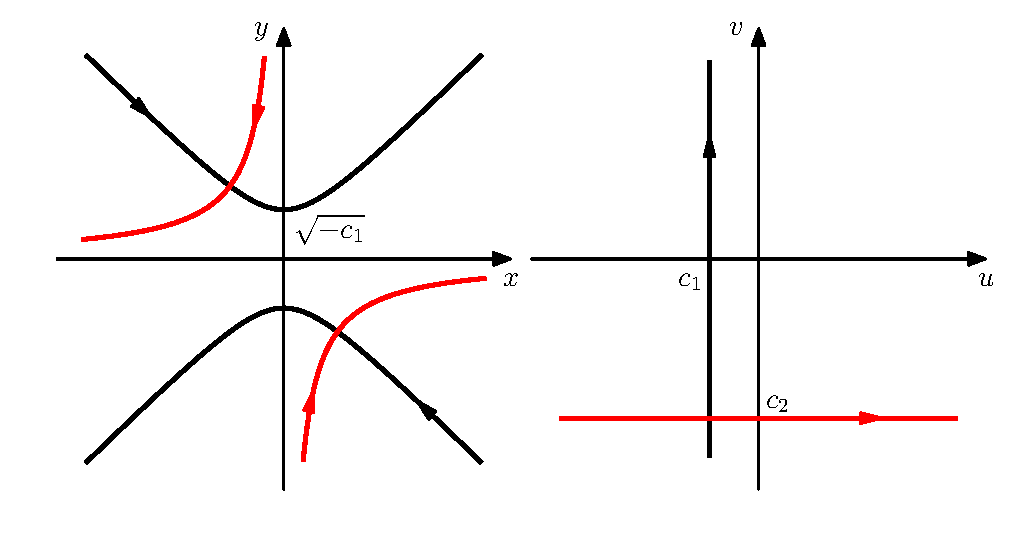
\includegraphics[width=0.85\textwidth]{figuras/exercise_14_06.pdf}
 \caption{\label{fig:exercise_14_06} Ejercicio 6. Imágenes de las hipérbolas rectangulares \(x^2-y^2=c_1\) con \(c_1<0\) y \(2xy=c_2\) con \(c_2<0\) bajo la transformación \(w=z^2\).}
 \end{center}
\end{figure}

Por otro lado, 
\[
 2xy=c_2,\qquad c_2<0
\]
es una hipérbola rectangular cuyas ramas están en el segundo y cuarto cuadrante, y la segunda ecuación en \ref{eq:square_mapping} indica que un punto en cualquier rama se transforma en un punto en la recta horizontal \(v=c_2\). La representación paramétrica de la rama del segundo cuadrante es
\[
 u=x^2-\frac{c_2^2}{4x^2},\qquad\qquad v=c_2\qquad\qquad\textrm{con}\qquad\qquad-\infty<x<0.
\]
Observando que 
\[
 \lim_{x\to-\infty}u=\infty
 \qquad\qquad\textrm{y}\qquad\qquad
 \lim_{x\to0^-}u=-\infty,
\]
como \(u\) es continua en \(x\), es claro que a medida que \((x,\,y)\) se mueve hacia abajo en la rama del segundo cuadrante, su imagen se mueve hacia la derecha sobre toda la recta \(v=c_2\). La representación paramétrica de la rama del cuarto cuadrante es
\[
 u=x^2-\frac{c_2^2}{4x^2},\qquad\qquad v=c_2\qquad\qquad\textrm{con}\qquad\qquad0<x<\infty,
\]
y como
\[
 \lim_{x\to0^+}u=-\infty
 \qquad\qquad\textrm{y}\qquad\qquad
 \lim_{x\to\infty}u=\infty,
\]
la imagen de un punto que se mueve hacia arriba en la rama del cuarto cuadrante es un punto que se mueve hacia la derecha en la recta \(v=c_2\), como se muestra en la figura \ref{fig:exercise_14_06}.

\subsubsection{Ejercicio 9}

Una interpretación de una función \(x=f(x,\,y)=u(x,\,y)+iv(x,\,y)\) es la de un \emph{campo vectorial} en el dominio de definición de \(f\). La función asigna un vector \(w\) con componentes \(u(x,\,y)\) y \(v(x,\,y)\) a cada punto \(z\) donde está definida. Indicar gráficamente los campos vectoriales representados por
\[
 (\textit{a})\;w=iz;\qquad\qquad (\textit{b})\;w=\frac{z}{|z|}.
\]
\paragraph{Solución}
\begin{enumerate}
 \item[(\textit{a})] Expresando \(z\) en coordenadas polares, \(z=re^{i\theta}\), y considerando que \(i=e^{i\pi/2}\), la transformación es
 \[
  w=iz=r\exp\left(\theta+\dfrac{\pi}{2}\right).
 \]
 Se observa que la transformación no altera el módulo y adiciona a la fase una magnitud de \(\pi/2\) radianes. Esto consiste en una rotación de \(\pi/2\) radianes en sentido antihorario del vector \(z\). El campo vectorial asociado a la transformación se muestra en la figura \ref{fig:exercise_14_09}.
 \item[(\textit{b})] La transformación \(w=z/|z|\) no altera la fase por tratarse únicamente de la división del vector \(z\) entre un número real y es tal que \(|w|=1\) para todo \(z\neq0\). El campo vectorial se muestra en la figura \ref{fig:exercise_14_09}.
\end{enumerate}
\begin{figure}[!htb]
 \begin{center}
 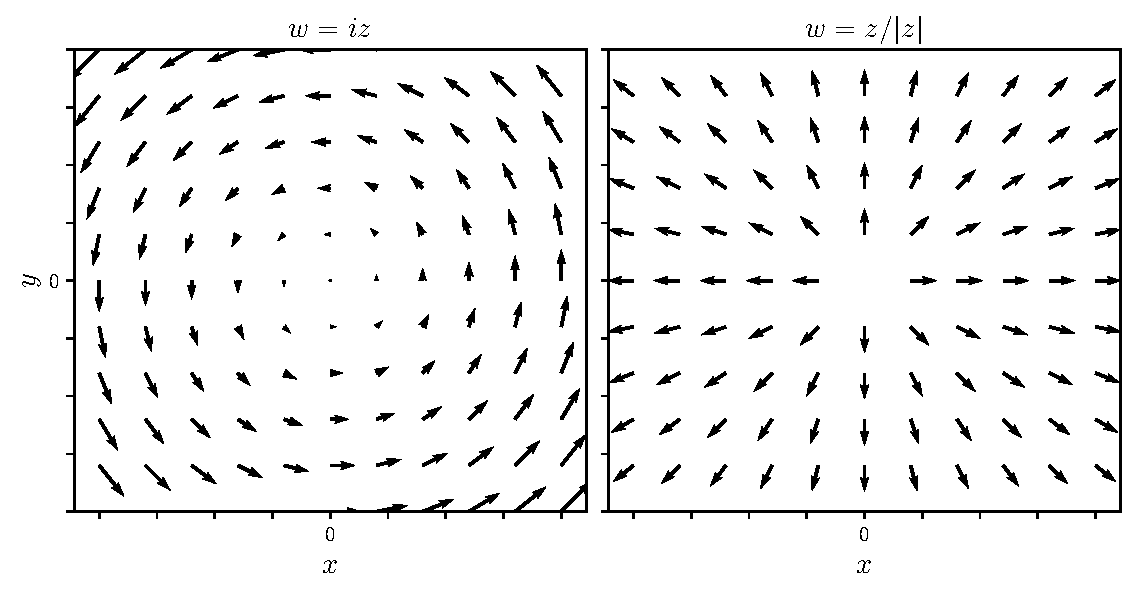
\includegraphics[width=0.9\textwidth]{figuras/exercise_14_09.pdf}
 \caption{\label{fig:exercise_14_09} Ejercicio 9. Campos vectoriales asociados a las transformaciones \(w=iz\) y \(w=z/|z|\).}
 \end{center}
\end{figure}

\section{Límites}

Sea una función \(f\) definida en todos los puntos \(z\) de un entorno reducido de un punto \(z_0\). La afirmación de que \(f(z)\) tiene límite \(w_0\) cuando \(z\) se aproxima a \(z_0\), o
\begin{equation}\label{eq:limit_statement}
 \lim_{z\to z_0}f(z)=w_0, 
\end{equation}
significa que el punto \(w=f(z)\) puede hacerse arbitrariamente cercano a \(w_0\) si se elige el punto \(z\) suficientemente cercano a \(z_0\) pero distinto de él. A continuación se expresa la definición formal.

La afirmación de la ecuación \ref{eq:limit_statement} significa que para cada número positivo \(\epsilon\), existe un número positivo \(\delta\) tal que
\begin{equation}\label{eq:limit_definition}
 |f(z)-w_0|<\epsilon\qquad\textrm{para todo }z\textrm{ tal que}\qquad0<|z-z_0|<\delta. 
\end{equation}
Geométricamente, la definición indica que para cada entorno de \(w_0\) de radio \(\epsilon\), \(|w-w_0|<\epsilon\), existe un entorno reducido de \(z_0\) de radio \(\delta\), \(0<|z-z_0|<\delta\), tal que cada punto \(z\) en él tiene su imagen \(w\) en el entorno de radio \(\epsilon\) de \(w_0\). Observar que si bien todos los puntos del entorno reducido \(0<|z-z_0|<\delta\) deben ser considerados, sus imágenes no tienen porque abarcar el entorno \(|w_0-w|<\epsilon\) completo. Notar además que una vez que se encontró un valor de \(\delta\) que cumpla la condición, puede ser sustituido por cualquier número positivo menor, como \(\delta/2\) por ejemplo.

\paragraph{Teorema: unicidad del límite.} Cuando el límite de una función \(f(z)\) existe en el punto \(z_0\), es único.\\[1ex]

La definición \ref{eq:limit_definition} requiere que \(f\) esté definida en todos los puntos del entorno reducido de \(z_0\). Dicho entorno reducido siempre existe si \(z_0\) es un punto interior de la región en donde \(f\) está definida. La definición de límite puede extenderse al caso en que \(z_0\) es un punto de la frontera de la región de definición de \(f\) acordando que la primera inecuación en \ref{eq:limit_definition} debe satisfacerse únicamente para los puntos \(z\) que pertenecen a intersección de la región de definición de \(f\) con entorno reducido.  

Si el limite \ref{eq:limit_statement} existe, la notación \(z\to z_0\) implica que \(z\) se aproxima a \(z_0\) de forma arbitraria y no en una dirección en particular. 

\section{Teoremas sobre límites}\label{sec:limits_theorems}

El estudio sobre límites puede abreviarse estableciendo una conexión entre el límite de funciones de variable compleja y el límite de funciones reales de dos variables reales. Como los límites del último tipo se estudian en cálculo, sus definiciones y propiedades pueden emplearse libremente. 

\paragraph{Teorema 1.} Supóngase que 
\[
 f(z)=u(x,\,y)+iv(x,\,y),\qquad\qquad\textrm{con}\qquad\qquad z=x+iy,
\]
y
\[
 z_0=x_0+iy_0,\qquad\qquad w_0=u_0+iv_0.
\]
Si
\[
 \lim_{(x,\,y)\to(x_0,\,y_0)}u(x,\,y)=u_0
 \qquad\qquad\textrm{y}\qquad\qquad
 \lim_{(x,\,y)\to(x_0,\,y_0)}v(x,\,y)=v_0
\]
se cumple que 
\[
 \lim_{z\to z_0}f(z)=w_0.
\]
Lo recíproco también es cierto.

\paragraph{Teorema 2.} Supóngase que
\[
 \lim_{z\to z_0}f(z)=w_0
 \qquad\qquad\textrm{y}\qquad\qquad
 \lim_{z\to z_0}F(z)=W_0.
\]
Entonces, se cumple que 
\begin{equation}\label{eq:limits_functions_operations}
 \lim_{z\to z_0}[f(z)+F(z)]=w_0+W_0,
 \qquad
 \lim_{z\to z_0}f(z)F(z)=w_0W_0
 \qquad\textrm{y}\qquad 
 \lim_{z\to z_0}\frac{f(z)}{F(z)}=\frac{w_0}{W_0},
\end{equation}
donde en el último límite se debe imponer la condición adicional de que \(W_0\neq0\).

\section{Límites que involucran el punto en el infinito}\label{sec:limits_infinity_point}

En ocasiones es conveniente incluir en el plano complejo el \emph{punto en el infinito}, denotado como \(\infty\), y emplear límites que lo involucran. El plano complejo en conjunto con este punto se denomina \emph{plano complejo extendido}. Para visualizar el punto en el infinito, se puede pensar en el plano complejo como pasando por el ecuador de una esfera unidad centrada en el origen, como se muestra en la figura \ref{fig:point_at_infinity_mayavi_v2_resize}. A cada punto \(z\) en el plano complejo le corresponde exactamente un punto \(P\) en la superficie de la esfera. El punto \(P\) es el punto donde la recta que pasa por \(z\) y el polo norte \(N\) intersecta la esfera. De forma similar, a cada punto \(P\) de la esfera, excepto al polo norte \(N\), le corresponde exactamente un punto \(z\)  en el plano complejo. Si se asigna al polo norte \(N\) de la esfera el punto en el infinito, se obtiene una correspondencia uno a uno entre puntos de la esfera y puntos del plano complejo extendido. La esfera se conoce como \emph{esfera de Riemann} y la correspondencia se llama \emph{proyección estereográfica}.
\begin{figure}[!htb]
 \begin{center}
 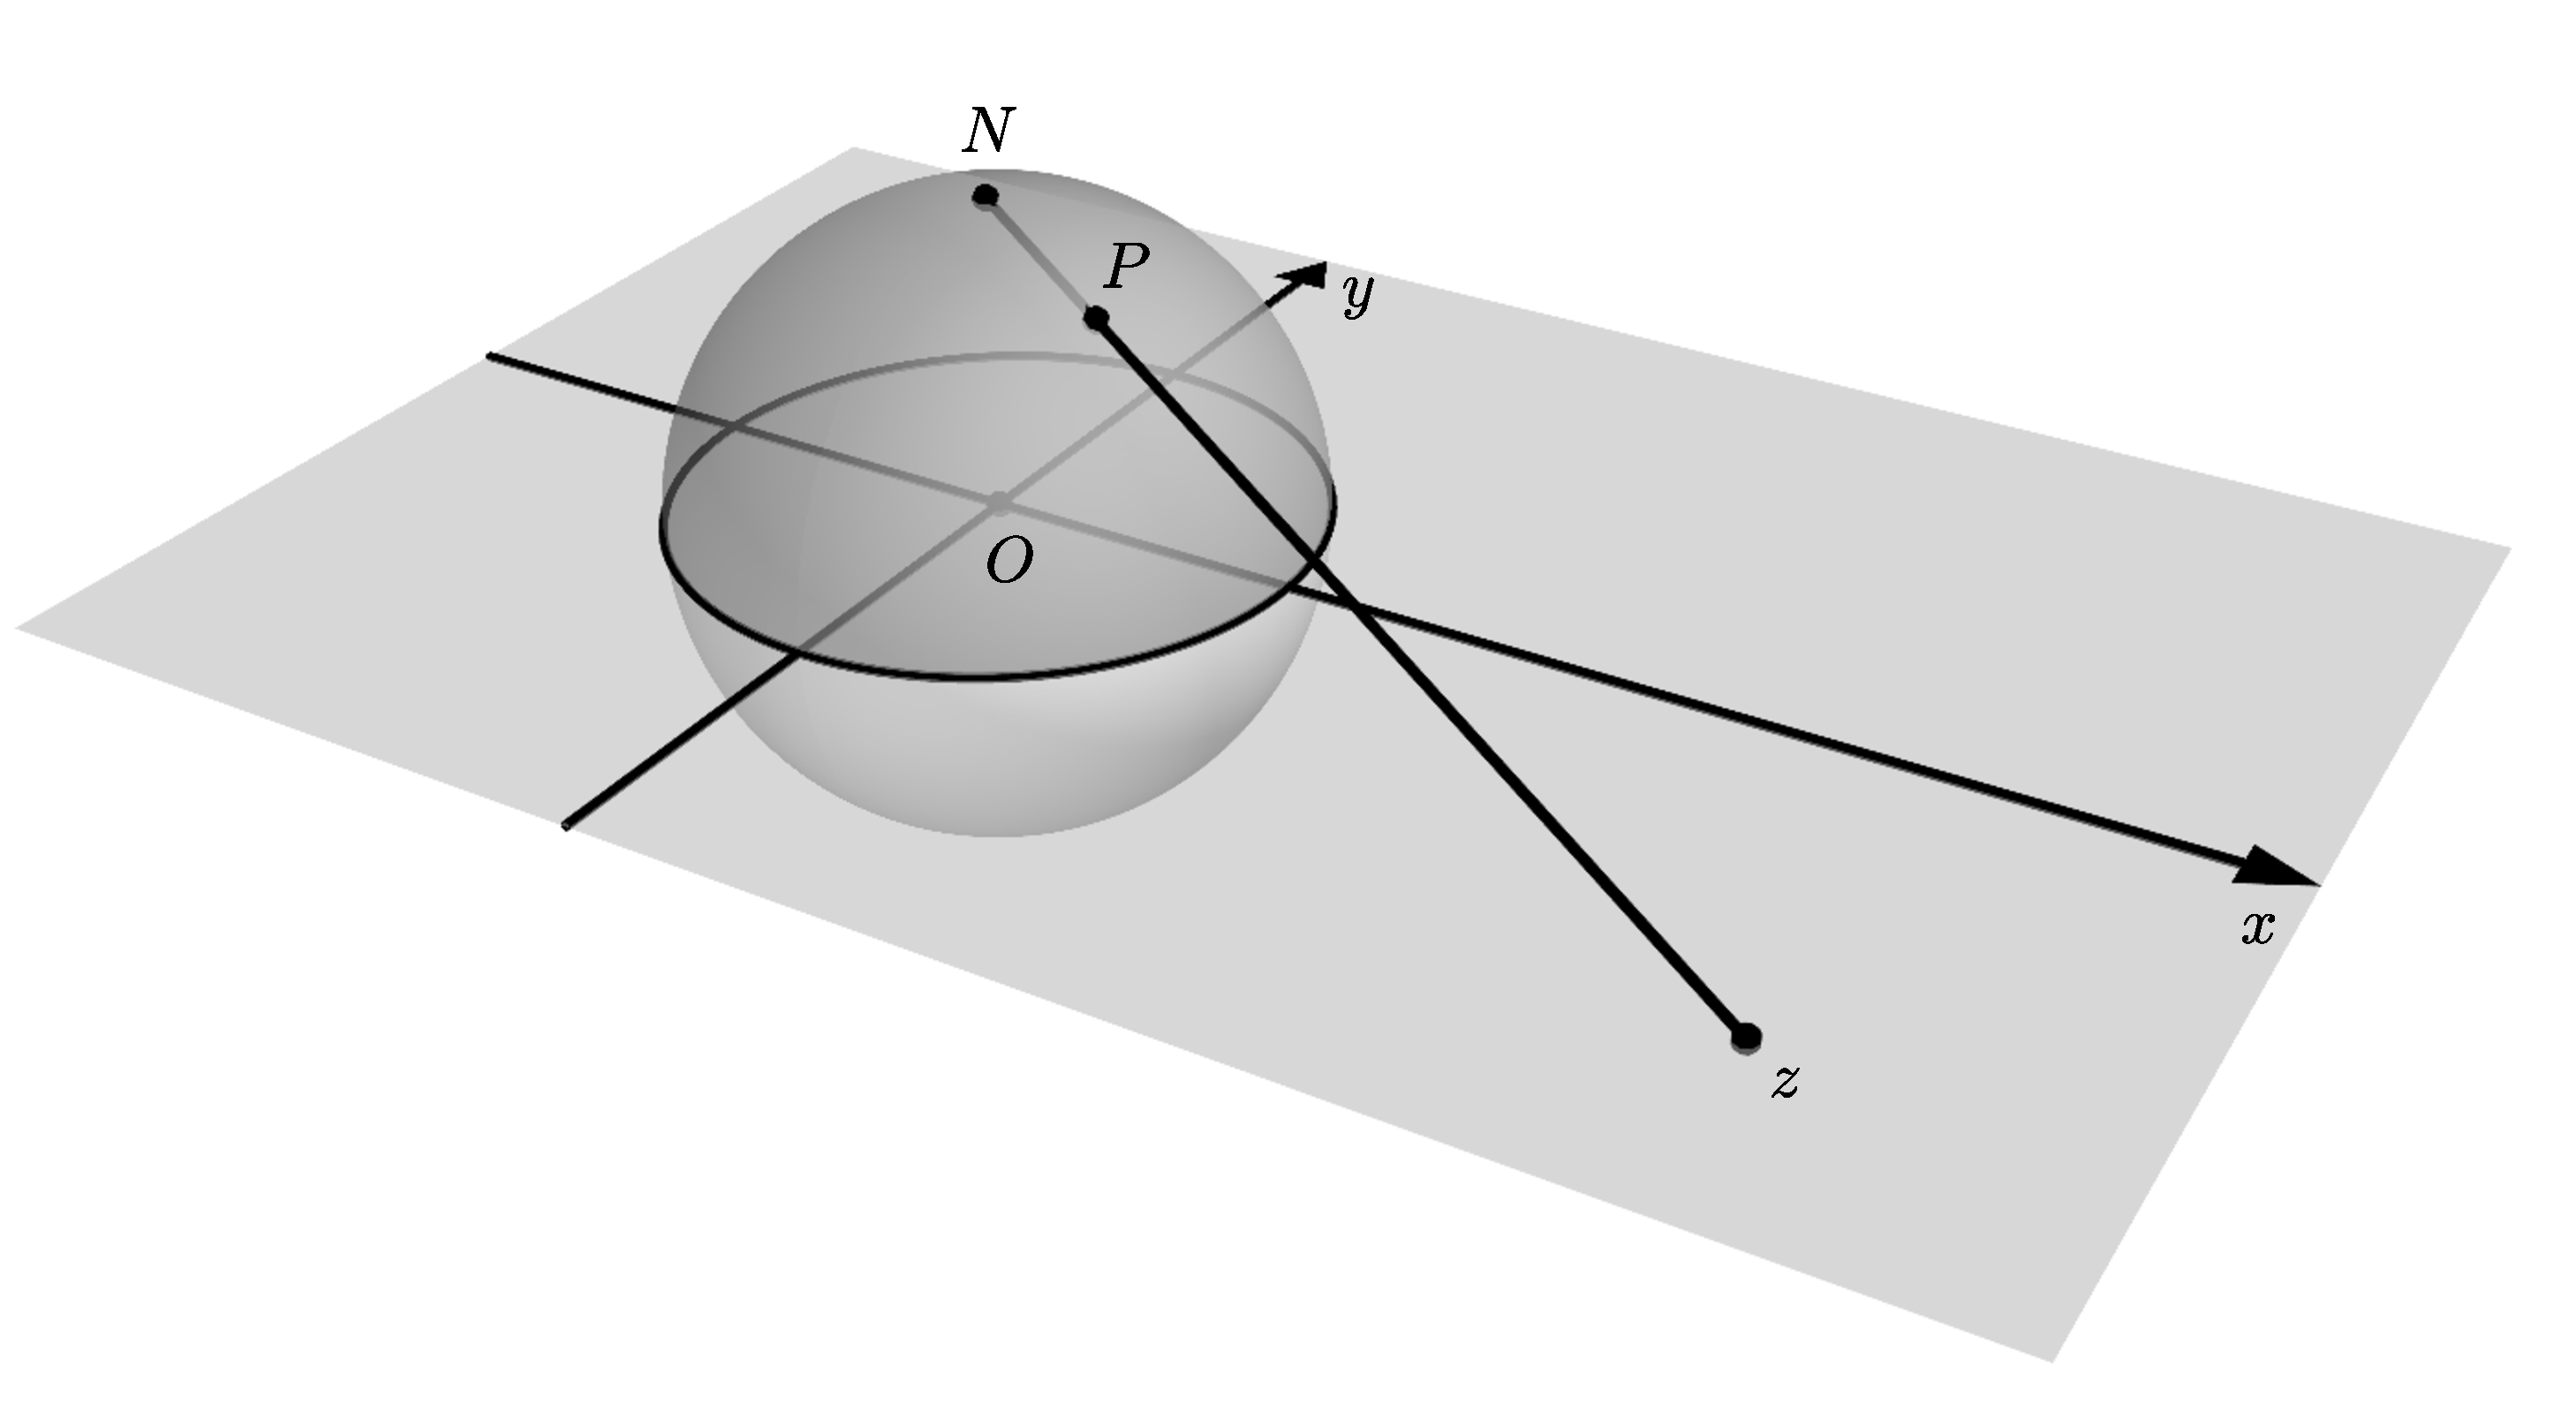
\includegraphics[width=0.95\textwidth]{figuras/point_at_infinity_mayavi_v2_resize.pdf}
 \caption{\label{fig:point_at_infinity_mayavi_v2_resize} Proyección estereográfica.}
 \end{center}
\end{figure}


Observar que el exterior del círculo unidad centrado en el origen en el plano complejo, corresponde al hemisferio norte con el ecuador y el polo norte \(N\) omitidos. Además, para cada número pequeño positivo \(\epsilon\), los puntos en el plano complejo exteriores a la circunferencia \(|z|=1/\epsilon\) corresponden a puntos en la esfera cercanos a \(N\). Por lo tanto, al conjunto \(|z|>1/\epsilon\) se le llama \emph{entorno de }\(\infty\).

Como convención, al referirse a un punto \(z\), se asumirá que se trata de un punto del \emph{plano finito}. Por lo tanto, cuando haya que referirse al punto en el infinito, se hará explícitamente.

Teniendo en cuenta estas consideraciones, ya es posible darle un significado a la afirmación
\[
 \lim_{z\to z_0} f(z)=w_0
\]
cuando \(z_0\) o \(w_0\), o posiblemente ambos números, son reemplazados por el punto en el infinito. Para hacerlo, en la definición del límite dada por la ecuación \ref{eq:limit_definition} simplemente se reemplaza el entorno correspondiente de \(z_0\) o \(w_0\) por un entorno de \(\infty\). La prueba del siguiente teorema ilustra como se hace.

\paragraph{Teorema.} Si \(z_0\) y \(w_0\) son puntos en el pano \(z\) y \(w\) respectivamente, entonces,
\[
 \lim_{z\to z_0} f(z)=\infty
  \qquad\qquad\textrm{si}\qquad\qquad
 \lim_{z\to z_0} \frac{1}{f(z)}=0 
\]
y
\[
 \lim_{z\to \infty} f(z)=w_0
  \qquad\qquad\textrm{si}\qquad\qquad
 \lim_{z\to 0}f\left(\frac{1}{z}\right)=w_0. 
\]
Además,
\[
 \lim_{z\to \infty} f(z)=\infty
  \qquad\qquad\textrm{si}\qquad\qquad
 \lim_{z\to 0}\frac{1}{f(1/z)}=0. 
\]
Se incluye a continuación la prueba solo de la primera afirmación. Asumiendo que se cumple el segundo límite en la primera afirmación, la definición de límite \ref{eq:limit_definition} indica que para todo número \(\epsilon\) positivo, existe un número \(\delta\) positivo tal que 
\[
 \left|\frac{1}{f(z)}-0\right|<\epsilon
 \qquad\textrm{si se cumple que}\qquad
 0<|z-z_0|<\delta.
\]
Como esto puede escribirse como
\[
 |f(z)|>\frac{1}{\epsilon}
 \qquad\textrm{si se cumple que}\qquad
 0<|z-z_0|<\delta,
\]
se obtiene el primer límite de la primera afirmación, ya que la expresión indica que \(f(z)\) se encuentra en un entorno de \(\infty\).

\section{Continuidad}\label{sec:continuity_definition}

Una función \(f\) es \emph{continua} en el punto \(z_0\) si se cumplen las siguientes tres condiciones:
\begin{enumerate}
 \item \(\displaystyle\lim_{z\to z_0}f(z)\) existe.
 \item \(\displaystyle f(z_0)\) existe.
 \item \(\displaystyle\lim_{z\to z_0}f(z)=f(z_0)\).
\end{enumerate}
Observar que la afirmación 3. contiene las afirmaciones 1. y 2., ya que la existencia de los valores en ambos lados de la igualdad de la ecuación es necesaria. La afirmación 3. indica que para todo numero \(\epsilon\) positivo existe un número \(\delta\) positivo tal que
\begin{equation}\label{eq:continuity_definition}
 |f(z)-f(z_0)|<\epsilon
 \qquad\textrm{si se cumple que}\qquad
 |z-z_0|<\delta.
\end{equation}

Una función de variable compleja se dice continua en una región \(R\) si es continua en cada punto de \(R\).

Si dos funciones son continuas en un punto, su suma y su producto también son continuas en ese punto, y su cociente es una función continua si el denominador no es cero en ese punto. Esto es consecuencia de la ecuación \ref{eq:limits_functions_operations}.

A continuación se incluyen otras propiedades de funciones continuas como teoremas, cuya verificación no es tan inmediata.

\paragraph{Teorema 1.} La composición de funciones continuas es una función continua. 

Sea \(w=f(z)\) una función definida para todo \(z\) en el entorno \(|z-z_0|<\delta\) del punto \(z_0\), y sea \(W=g(w)\) una función cuyo dominio de definición contiene la imagen de dicho entorno bajo \(f\). De esta forma, la composición \(W=g[f(z)]\) está definida para todo el entorno \(|z-z_0|<\delta\). Si \(f\) es continua en \(z_0\) y \(g\) es continua en el punto \(f(z_0)\) del plano \(w\), se cumple que \(g[f(z)]\) es continua en \(z_0\).

\paragraph{Teorema 2.} Si una función \(f(z)\) es continua y no nula en el punto \(z_0\), entonces \(f(z)\neq0\) en algún entorno de ese punto.

\paragraph{Teorema 3.} Sea
\[
 f(z)=u(x,\,y)+iv(x,\,y).
\]
Si las funciones componentes \(u\) y \(v\) son continuas en el punto \(z_0=(x_0,\,y_0)\), también los es \(f\). Recíprocamente, si \(f\) es continua en el punto \(z_0\), también los son \(u\) y \(v\) en ese punto.

\paragraph{Teorema 4.} Si una función \(f\) es continua en una región \(R\) cerrada y acotada, existe un número \(M\) no negativo tal que 
\[
 |f(z)|\leq M\qquad\textrm{para todos los puntos }z\textrm{ en }R,
\]
y la igualdad se cumple para al menos un punto \(z\) de \(R\). En estas condiciones, se dice que \(f\) es \emph{acotada en }\(R\).

\subsection*{Ejercicios}

\subsubsection{Ejercicio 1}

Emplear la definición de límite dada por la ecuación \ref{eq:limit_definition} para probar que 
\[
 (\textit{a})\;\lim_{z\to z_0}\Re z=\Re z_0;\qquad\qquad 
 (\textit{b})\;\lim_{z\to z_0}\overline{z}=\overline{z_0};\qquad\qquad
 (\textit{c})\;\lim_{z\to z_0}\frac{\overline{z}^2}{z}=0.
\]

\paragraph{Solución} 
\begin{enumerate}
 \item[(\textit{a})] Hay que probar que para todo número \(\epsilon\) positivo, existe un número \(\delta\) positivo tal que 
\begin{equation}\label{eq:exersice_18_01_a_limit}
 |\Re z-\Re z_0|<\epsilon
 \qquad\textrm{si se cumple que}\qquad
 0<|z-z_0|<\delta.
\end{equation}
Sea \(z=x+iy\) y \(z_0=x_0+iy_0\). De esta forma,
\[
 |\Re z-\Re z_0|=|x-x_0|.
\]
Por otro lado,
\[
 |z-z_0|=|(x+iy)-(x_0+iy_0)|=|(x-x_0)+i(y-y_0)|\geq|x-x_0|
\]
Combinando los resultados, se tiene que 
\[
 |\Re z-\Re z_0|=|x-x_0|\leq|z-z_0|.
\]
Por lo tanto, eligiendo \(\delta=\epsilon\) se cumple \ref{eq:exersice_18_01_a_limit} para todo \(\epsilon>0\).
\item[(\textit{b})] Hay que probar que para todo \(\epsilon>0\), existe \(\delta\) tal que
\begin{equation}\label{eq:exersice_18_01_b_limit}
 |\overline{z}-\overline{z_0}|<\epsilon
 \qquad\textrm{si se cumple que}\qquad
 0<|z-z_0|<\delta.
\end{equation}
Como 
\[
 |\overline{z}-\overline{z_0}|=|\overline{(z-z_0)}|=|z-z_0|,
\]
eligiendo \(\delta=\epsilon\), se cumple la ecuación \ref{eq:exersice_18_01_b_limit} para todo \(\epsilon>0\).
\item[(\textit{c})] Hay que probar que para todo \(\epsilon>0\), existe \(\delta\) tal que
\begin{equation}\label{eq:exersice_18_01_c_limit}
 \left|\frac{\overline{z}^2}{z}-0\right|<\epsilon
 \qquad\textrm{si se cumple que}\qquad
 0<|z-0|<\delta.
\end{equation}
Observando que 
\[
 \left|\frac{\overline{z}^2}{z}-0\right|=\left|\frac{\overline{z}^2}{z}\right|=\frac{|\overline{z}|^2}{|z|}=\frac{|z|^2}{|z|}=|z|,
\]
eligiendo \(\delta=\epsilon\), se cumple la ecuación \ref{eq:exersice_18_01_c_limit} para todo \(\epsilon>0\).
\end{enumerate}

\subsubsection{Ejercicio 2}

Sean las constantes complejas \(a\), \(b\) y \(c\). Emplear la definición de límite dada por la ecuación \ref{eq:limit_definition} para probar que 
\begin{align*}
 (\textit{a})\;&\lim_{z\to z_0}(az+b)=az_0+b;\qquad\qquad\qquad
 (\textit{b})\;\lim_{z\to z_0}(z^2+c)=z_0^2+c;\\
 (\textit{c})\;&\lim_{z\to1-i}x+i(2x+y)=1+i,\qquad\textrm{con}\qquad z=x+iy.
\end{align*}

\paragraph{Solución} 
\begin{enumerate}
 \item[(\textit{a})] Sea \(\epsilon>0\) y supóngase que \(|z-z_0|<\delta\). Si \(a=0\), se cumple que 
 \[
  |(az+b)-(az_0+b)|=|b-b|=0<\epsilon.
 \]
 Si \(a\neq0\),
 \[
  |(az+b)-(az_0+b)|=|a||z-z_0|<|a|\delta.
 \]
 Por lo tanto, eligiendo \(\delta=\epsilon/|a|\), se cumple que 
 \[
  |(az+b)-(az_0+b)|<\epsilon
  \qquad\textrm{si se cumple que}\qquad
  0<|z-z_0|<\delta=\frac{\epsilon}{|a|}.
 \]
 \item[(\textit{b})] Sea \(\epsilon>0\) y supóngase que \(|z-z_0|<\delta\). Se observa que
 \begin{align*}
  |(z^2+c)-(z_0^2+c)|&=|z^2-z_0^2|\\
   &=|z+z_0||z-z_0|\\
   &=|z-z_0+2z_0||z-z_0|\\
   &\leq(|z-z_0|+2|z_0|)|z-z_0|\\
   &<(\delta+2|z_0|)\delta.
 \end{align*}
 Por lo tanto, eligiendo \(\delta\) tal que \((\delta+2|z_0|)\delta=\epsilon\), es decir, \(\delta=\sqrt{|z_0|^2+\epsilon}-|z_0|\), se cumple que 
 \[
  |(z^2+c)-(z_0^2+c)|<\epsilon
  \qquad\textrm{si se cumple que}\qquad
  0<|z-z_0|<\delta.
 \]
 
 A continuación se resolverá el problema de forma alternativa para obtener un resultado mas simple. El método es clásico en las pruebas \emph{epsilon-delta}. Se parte igual que antes planteando la condición \(|f(z)-w_0|<\epsilon\), que en este caso es
 \begin{equation}\label{eq:exersice_18_02_b_epsilon_condition}
  |(z^2+c)-(z_0^2+c)|=|z^2-z_0^2|=|z+z_0||z-z_0|<\epsilon,
 \end{equation}
 y al despejar el término \(|z-z_0|\), la condición queda
 \begin{equation}\label{eq:exersice_18_02_b_delta_condition}
  |z-z_0|<\frac{\epsilon}{|z+z_0|}.
 \end{equation}
 De esta forma, podría establecerse \(\delta=\epsilon/|z+z_0|\), pero \(\delta\) debe depender solo de \(\epsilon\) y no de otras variables, por lo que hay que eliminar el factor \(|z+z_0|\). Para hacerlo, se considera que el concepto de límite se aplica solo cuando \(z\) es suficientemente cercano a \(z_0\), por lo que se restringirá al caso en que \(z\) diste a los sumo 1 de \(z_0\), es decir, \(|z-z_0|<1\). Así, el término \(|z+z_0|\) cumple que
 \[
  |z+z_0|=|z-z_0+2z_0|\leq|z-z_0|+2|z_0|<1+2|z_0|,
 \]
 donde la última desigualdad proviene de la condición \(|z-z_0|<1\). Se obtuvo que
 \begin{equation}\label{eq:exersice_18_02_b_z_condition}
  |z+z_0|<1+2|z_0|.
 \end{equation}
 Ahora, el lado derecho de la ecuación \ref{eq:exersice_18_02_b_delta_condition} es mínimo cuando de denominador es máximo, por lo que sustituyendo el resultado de la ecuación \ref{eq:exersice_18_02_b_z_condition} resulta en
 \[
  |z-z_0|<\frac{\epsilon}{1+2|z_0|}.
 \]
 Como se tienen las dos condiciones
 \[
  |z-z_0|<1
   \qquad\qquad\textrm{y}\qquad\qquad
  |z-z_0|<\frac{\epsilon}{1+2|z_0|},
 \]
 se elige
 \[
  \delta=\min\left\{1,\,\frac{\epsilon}{1+2|z_0|}\right\}.
 \]
 Finalmente, se verificará que con esta elección de \(\delta\), se satisface la condición \ref{eq:exersice_18_02_b_epsilon_condition}.
 \begin{itemize}
  \item Se considera el caso en que \(\delta=1\) y por lo tanto
  \[
   1<\frac{\epsilon}{1+2|z_0|},
   \qquad\qquad\textrm{es decir}\qquad\qquad 1+2|z_0|<\epsilon.
  \]
  La condición \(|z-z_0|<\delta\) es en este caso \(|z-z_0|<1\), por lo que multiplicando por \(|z+z_0|\) a ambos lados de la inecuación, se tiene que 
  \[
   |z-z_0||z+z_0|<|z+z_0|\overset{(a)}{<}1+2|z_0|<\epsilon,
  \]
  donde en \((a)\) se empleó la ecuación \ref{eq:exersice_18_02_b_z_condition}. Esto indica que se cumple que \(|f(z)-w_0|<\epsilon\) si \(|z-z_0|<\delta\), como se requiere.
  \item Sea ahora
  \[
   \delta=\frac{\epsilon}{1+2|z_0|}.
  \]
  La condición \(|z-z_0|<\delta\) es en este caso
  \[
   |z-z_0|<\frac{\epsilon}{1+2|z_0|},
  \]
  y al multiplicar por \(|z+z_0|\) a ambos lados de la inecuación se obtiene que 
  \[
   |z-z_0||z+z_0|<\frac{\epsilon}{1+2|z_0|}|z+z_0|\overset{(a)}{<}\frac{\epsilon}{1+2|z_0|}(1+2|z_0|)=\epsilon,
  \]
  donde en \((a)\) se empleó la ecuación \ref{eq:exersice_18_02_b_z_condition}.
 \end{itemize} 
 \item[(\textit{c})] Sea \(z=x+iy\). Hay que probar que para todo \(\epsilon>0\), existe \(\delta>0\) tal que
 \begin{equation}\label{eq:exersice_18_02_c_limit}
  |[x+i(2x+y)]-(1+i)|<\epsilon
  \qquad\textrm{si se cumple que}\qquad
  0<|(x+iy)-(1-i)|<\delta.
 \end{equation}
 Por un lado se tiene que 
 \[
  |(x+iy)-(1-i)|=|(x-1)+i(y-1)|,
 \]
 y por lo tanto, asumiendo que
 \begin{equation}\label{eq:exersice_18_02_c_delta_condition}
  |(x+iy)-(1-i)|<\delta
  \qquad\textrm{se cumple que}\qquad
  |x-1|<\delta\qquad\textrm{y}\qquad|y+1|<\delta.
 \end{equation}
 Por otro lado, se observa que 
 \begin{align*}
  |[x+i(2x+y)]-(1+i)|&=|(x-1)+i(2x+y-1)|\\
   &\leq|x-1|+|2x+y-1|\\
   &=|x-1|+|2x-2+y+1|\\
   &\leq|x-1|+2|x-1|+|y+1|\\
   &\overset{(a)}{<}\delta+2\delta+\delta\\
   &=4\delta,
 \end{align*}
 donde en \((a)\) se asumió que se cumple la condición de la ecuación \ref{eq:exersice_18_02_c_delta_condition}. Por lo tanto, eligiendo \(\delta=\epsilon/4\), se cumple \ref{eq:exersice_18_02_c_limit}.
\end{enumerate}

\subsubsection{Ejercicio 3}

Sea \(n\) un entero positivo y sean \(P(z)\) y \(Q(z)\) polinomios, con \(Q(z_0)\neq0\). Emplear los resultados del teorema que conduce a la ecuación \ref{eq:limits_functions_operations} para encontrar
\[
 (\textit{a})\;\lim_{z\to z_0}\frac{1}{z^n};\qquad\qquad 
 (\textit{b})\;\lim_{z\to i}\frac{iz^3-1}{z+i};\qquad\qquad
 (\textit{c})\;\lim_{z\to z_0}\frac{P(z)}{Q(z)}.
\]

\paragraph{Solución} 

\begin{enumerate}
 \item[(\textit{a})] 
 \(\displaystyle\lim_{z\to z_0}\frac{1}{z^n}=\frac{1}{\lim\limits_{z\to z_0}z^n}=\frac{1}{z_0^n}\)
 \item[(\textit{b})] 
 \(\displaystyle\lim_{z\to i}\frac{iz^3-1}{z+i}=\frac{\lim\limits_{z\to i}iz^3-1}{\lim\limits_{z\to i}z+i}=\frac{i(i^3)-1}{i+i}=\frac{1-1}{2i}=0\).
 \item[(\textit{c})]
 \(\displaystyle\lim_{z\to z_0}\frac{P(z)}{Q(z)}=\frac{\lim\limits_{z\to z_0}P(z)}{\lim\limits_{z\to z_0}Q(z)}=\frac{P(z_0)}{Q(z_0)}\).
\end{enumerate}

\subsubsection{Ejercicio 4}

Emplear inducción matemática y el resultado de la ecuación \ref{eq:limits_functions_operations} para mostrar que
\begin{equation}\label{eq:exersice_18_04_objective}
 \lim_{z\to z_0}z^n=z_0^n,
\end{equation}
donde \(n\) es un entero positivo.

\paragraph{Solución} Se considera primero el \emph{caso base} en que \(n=1\). Consiste en probar que 
\[
 \lim_{z-z_0}z=z_0,
\]
lo que es directo: es fácil ver que alcanza con elegir \(\delta=\epsilon\) en la definición de límite dada por la ecuación \ref{eq:limit_definition}. El \emph{paso inductivo} consiste en mostrar que si la ecuación \ref{eq:exersice_18_04_objective} se cumple para \(n=k\), se cumple para \(n=k+1\), es decir,
\[
 \lim_{z\to z_0}z^k=z_0^k
 \qquad\qquad\Rightarrow\qquad\qquad
 \lim_{z\to z_0}z^{k+1}=z_0^{k+1}.
\] 
Como
\[
 \lim_{z\to z_0}z^{k+1}=\lim_{z\to z_0}z^kz\overset{(a)}{=}\left(\lim_{z\to z_0}z^k\right)\left(\lim_{z\to z_0}z\right)\overset{(b)}{=}z_0^kz_0=z_0^{k+1},
\]
donde en \((a)\) se empleó el resultado de la ecuación \ref{eq:limit_definition} y en \((b)\) se empleó el caso base y la hipótesis de inducción, concluyendo la prueba.

\subsubsection{Ejercicio 5}

Mostrar que la función
\[
 f(z)=\left(\frac{z}{\overline{z}}\right)^2
\]
tiene valor 1 en todos los puntos no nulos de los ejes real e imaginario, donde \(z=(x,\,0)\) y \(z=(0,\,y)\) respectivamente, pero tiene valor \(-1\) en todos los puntos no nulos de la recta \(y=x\), donde \(z=(x,\,x)\). Esto muestra que el límite de \(f(z)\) cuando \(z\) tiende a 0 no existe. Observar que no es suficiente considerar únicamente los puntos no nulos \(z=(x,\,0)\) y \(z=(0,\,y)\) por ejemplo.

\paragraph{Solución} Con \(z=x+iy\),
\[
 f(z)=\left(\frac{z}{\overline{z}}\right)^2=\left(\frac{x+iy}{x-iy}\right)^2.
\]
En el caso en que \(z=(x,\,0)\), se tiene que 
\[
 f(z)=\left(\frac{x+i0}{x-i0}\right)^2=1.
\]
En el caso en que \(z=(0,\,y)\), se cumple que 
\[
 f(z)=\left(\frac{0+iy}{0-iy}\right)^2=1.
\]
Pero si \(z=(x,\,x)\),
\[
 f(z)=\left(\frac{x+ix}{x-ix}\right)^2=\frac{x^2-x^2+2ix^2}{x^2-x^2-2ix^2}=-1.
\]
Como \(f(z)\) tiene valor 1 en todos los puntos del eje real e imaginario exceptuando el origen y tiene valor \(-1\) en la recta \(y=x\) exceptuando el origen, el límite de \(f(z)\) cuando \(z\) tiende a 0 no puede existir.

\subsubsection{Ejercicio 6}

Probar la afirmación
\[
 \lim_{z\to z_0}[f(z)+F(z)]=w_0+W_0
\]
de la ecuación \ref{eq:limits_functions_operations} mediante:
\begin{enumerate}
 \item[(\textit{a})] el teorema 1 de la sección \ref{sec:limits_theorems} y empleando propiedades del límite de funciones reales de dos variables reales.
 \item[(\textit{b})] la definición \ref{eq:limit_definition} del límite.
\end{enumerate}

\paragraph{Solución} 

\begin{enumerate}
 \item[(\textit{a})] Hay que probar que si
 \[
  \textrm{si}\qquad
  \begin{array}{l}
   \displaystyle\lim_{z\to z_0}f(z)=w_0\\[\medskipamount]
   \displaystyle\lim_{z\to z_0}F(z)=W_0
  \end{array}
  \qquad\qquad\Rightarrow\qquad\qquad 
  \lim_{z\to z_0}[f(z)+F(z)]=w_0+W_0.
 \]
 Sea \(z=x+iy\) y
 \[
 \begin{array}{c}
  f(z)=u(x,\,y)+iv(x,\,y),\qquad\qquad F(z)=U(x,\,y)+iV(x,\,y)\\[\medskipamount]
  z_0=x_0+iy_0,\qquad\qquad w_0=u_0+iv_0,\qquad\qquad W_0=U_0+iV_0.
 \end{array}
 \]
 Por el teorema 1 de la sección \ref{sec:limits_theorems} se cumple que 
 \[
  \begin{array}{lllll}
   \lim\limits_{z\to z_0}f(z)=w_0 & \qquad\Leftrightarrow & \qquad\lim\limits_{(x,\,y)\to(x_0,\,y_0)}u(x,\,y)=u_0 & \quad\textrm{y} &
  \quad\lim\limits_{(x,\,y)\to(x_0,\,y_0)}v(x,\,y)=v_0\\[\bigskipamount]
  \lim\limits_{z\to z_0}F(z)=W_0 & \qquad\Leftrightarrow & \qquad\lim\limits_{(x,\,y)\to(x_0,\,y_0)}U(x,\,y)=U_0 & \quad\textrm{y} &
  \quad\lim\limits_{(x,\,y)\to(x_0,\,y_0)}V(x,\,y)=V_0
  \end{array}
 \]
 y por la ley del límite de la suma de funciones reales se cumple que 
 \begin{equation}\label{eq:exersice_18_06_sum_law}
  \lim_{(x,\,y)\to(x_0,\,y_0)}[u(x,\,y)+U(x,\,y)]=u_0+U_0
  \qquad\textrm{y}\qquad
  \lim_{(x,\,y)\to(x_0,\,y_0)}[v(x,\,y)+V(x,\,y)]=v_0+V_0.
 \end{equation}
 Por otro lado, se tiene que 
 \begin{align*}
  f(z)+F(z)&=[u(x,\,y)+iv(x,\,y)]+[U(x,\,y)+iV(x,\,y)]\\
    &=[u(x,\,y)+U(x,\,y)]+i[v(x,\,y)+V(x,\,y)],
 \end{align*}
y por lo tanto,
\begin{align*}
 \lim_{z\to z_0}f(z)+F(z)&=\lim_{(x,\,y)\to(x_0,\,y_0)}\left\{[u(x,\,y)+U(x,\,y)]+i[v(x,\,y)+V(x,\,y)]\right\}\\
  &\overset{(a)}{=}[u_0+U_0]+i[v_0+V_0]\\
  &=[u_0+iv_0]+[U_0+iV_0]\\
  &=w_0+iW_0.
\end{align*}
donde en \((a)\) se empleó el teorema 1 de la sección \ref{sec:limits_theorems} y el resultado de la ecuación \ref{eq:exersice_18_06_sum_law}, concluyendo la prueba. 
 \item[(\textit{b})] Considerando la definición \ref{eq:limit_definition} del límite, hay que probar que para todo \(\epsilon>0\), existe \(\delta>0\) tal que si \(0<|z-z_0|<\delta\), se cumple que \(|[f(z)+F(z)]-[w_0+W_0]|<\epsilon\). Aplicando la definición de límite a la hipótesis, se sabe que
 \[
 \begin{array}{lllll}
  \lim\limits_{z\to z_0}f(z)=w_0 & \qquad\Rightarrow & \qquad|f(z)-w_0|<\dfrac{\epsilon}{2}&\textrm{para todo }z\textrm{ tal que}&0<|z-z_0|<\delta_1\\[\bigskipamount]
  \lim\limits_{z\to z_0}F(z)=W_0 & \qquad\Rightarrow & \qquad|F(z)-W_0|<\dfrac{\epsilon}{2}&\textrm{para todo }z\textrm{ tal que}&0<|z-z_0|<\delta_2.
 \end{array} 
 \]
 Como
 \[
  |[f(z)+F(z)]-[w_0+W_0]|=|[f(z)-w_0]+[F(z)-W_0]|\leq|f(z)-w_0|+|F(z)-W_0|,
 \]
 eligiendo \(\delta=\min\{\delta_1,\,\delta_2\}\), se cumple que 
 \[
  |[f(z)+F(z)]-[w_0+W_0]|\leq|f(z)-w_0|+|F(z)-W_0|<\frac{\epsilon}{2}+\frac{\epsilon}{2}=\epsilon,
 \]
 que es lo que se quería demostrar.
\end{enumerate}

\subsubsection{Ejercicio 7}

Emplear la definición \ref{eq:limit_definition} de límite para mostrar que 
\[
 \textrm{si}\qquad\lim_{z\to z_0}f(z)=w_0
  \qquad\qquad\Rightarrow\qquad\qquad
 \lim_{z\to z_0}|f(z)|=|w_0|.
\]

\paragraph{Solución} Se probará primero la desigualdad 
\begin{equation}\label{eq:reverse_trinagle_inequality}
 ||z_1|-|z_2||\leq|z_1-z_2|,
\end{equation}
referida como \emph{desigualdad triangular inversa}\footnote{Ver \url{https://en.wikipedia.org/wiki/Triangle_inequality\#Reverse_triangle_inequality}, por ejemplo.}. Para hacerlo, se observa que 
\[
 \begin{array}{lll}
  |z_1|=|(z_1-z_2)+z_2|\leq|z_1-z_2|+|z_2| & \qquad\Rightarrow &\qquad |z_1|-|z_2|\leq|z_1-z_2|\\[\medskipamount]
  |z_2|=|(z_2-z_1)+z_1|\leq|z_2-z_1|+|z_1| & \qquad\Rightarrow &\qquad |z_1|-|z_2|\geq-|z_1-z_2|.
 \end{array}
\]
Por lo tanto
\[
 -|z_1-z_2|\leq|z_1|-|z_2|\leq|z_1-z_2|\qquad\Rightarrow\qquad ||z_1|-|z_2||\leq|z_1-z_2|,
\]
concluyendo la prueba.

Comenzando con el ejercicio, hay que mostrar que para cada número positivo \(\epsilon\), existe un número positivo \(\delta\) tal que
\[
 ||f(z)|-|w_0||<\epsilon\qquad\textrm{para todo }z\textrm{ tal que}\qquad0<|z-z_0|<\delta, 
\]
sabiendo que existe un número positivo \(\delta_2\) tal que
\[
 |f(z)-w_0|<\epsilon\qquad\textrm{para todo }z\textrm{ tal que}\qquad0<|z-z_0|<\delta_1. 
\]
De la ecuación \ref{eq:reverse_trinagle_inequality} y la hipótesis se deduce que  
\[
 ||f(z)|-|w_0||\leq|f(z)-w_0|<\epsilon,
\]
si \(\delta=\delta_1\).

\subsubsection{Ejercicio 8}

Definiendo \(\Delta z=z-z_0\), mostrar que 
\[
 \lim_{z\to z_0}f(z)=w_0
 \qquad\qquad\Leftrightarrow\qquad\qquad
 \lim_{\Delta z\to 0}f(z_0+\Delta z)=w_0.
\]

\paragraph{Solución} Empleando la definición \ref{eq:limit_definition} de límite hay que probar que para todo \(\epsilon>0\) existe \(\delta_1>0\) tal que
\[
 |f(z)-w_0|<\epsilon\qquad\textrm{para todo }z\textrm{ tal que}\qquad0<|z-z_0|<\delta_1, 
\]
si y solo si existe \(\delta_2\) tal que
\[
 |f(z_0+\Delta z)-w_0|<\epsilon\qquad\textrm{para todo }\Delta z\textrm{ tal que}\qquad0<|\Delta z-0|<\delta_2. 
\]
La demostración es inmediata sustituyendo \(\Delta z=z-z_0\) y tomando \(\delta=\delta_1=\delta_2\). 

\subsubsection{Ejercicio 9} 

Mostrar que 
\[
 \lim_{z\to z_0}f(z)g(z)=0
  \qquad\qquad\textrm{si}\qquad\qquad
 \lim_{z\to z_0}f(z)=0 
\]
y si existe un número positivo \(M\) tal que \(|g(z)|\leq M\) para todo \(z\) en algún entorno de \(z_0\).

\paragraph{Solución} Empleando la definición \ref{eq:limit_definition} de límite hay que probar que para todo \(\epsilon>0\) existe \(\delta>0\) tal que
\[
 |f(z)g(z)-0|<\epsilon\qquad\textrm{para todo }z\textrm{ tal que}\qquad0<|z-z_0|<\delta. 
\]
Pero por hipótesis se sabe que existe \(\delta_1\) tal que 
\[
 |g(z)|\leq M\qquad\textrm{para todo }z\textrm{ tal que}\qquad0<|z-z_0|<\delta_1
\]
y además que para todo \(\epsilon>0\), existe \(\delta_2>0\) tal que 
\[
 |f(z)-0|<\frac{\epsilon}{M}\qquad\textrm{para todo }z\textrm{ tal que}\qquad0<|z-z_0|<\delta_2. 
\]
Por lo tanto
\[
 |f(z)g(z)-0|=|f(z)||g(z)|<\frac{\epsilon}{M}M=\epsilon
\]
si se elige \(\delta=\min\{\delta_1,\,\delta_2\}\). Esto concluye la prueba.

\subsubsection{Ejercicio 10} 

Empleando el teorema de la sección \ref{sec:limits_infinity_point}, mostrar que 
\[
 (\textit{a})\;\lim_{z\to\infty}\frac{4z^2}{(z-1)^2}=4;\qquad\qquad 
 (\textit{b})\;\lim_{z\to1}\frac{1}{(z-1)^3}=\infty;\qquad\qquad
 (\textit{c})\;\lim_{z\to\infty}\frac{z^2+1}{z-1}=\infty.
\]

\paragraph{Solución} 

\begin{enumerate}
 \item[(\textit{a})]
 \(\displaystyle
 \lim_{z\to\infty}\frac{4z^2}{(z-1)^2}=\lim_{z\to0}\dfrac{4\left(\dfrac{1}{z}\right)^2}{\left(\dfrac{1}{z}-1\right)^2}=\lim_{z\to0}\frac{4}{(1-z)^2}=4
 \)
 \item[(\textit{b})]
 \(\displaystyle
  \lim_{z\to1}(z-1)^3=0
  \qquad\qquad\Leftrightarrow\qquad\qquad
  \lim_{z\to1}\frac{1}{(z-1)^3}=\infty.
 \)
 \item[(\textit{c})]
 \(\displaystyle
  \lim_{z\to0}\dfrac{\dfrac{1}{z}-1}{\left(\dfrac{1}{z}\right)^2+1}
  =\lim_{z\to0}\dfrac{1-z}{\dfrac{1+z^2}{z}}
  =\lim_{z\to0}\dfrac{z(1-z)}{1+z^2}=0
  \qquad\qquad\Leftrightarrow\qquad\qquad
  \lim_{z\to\infty}\frac{z^2+1}{z-1}=\infty.
 \)
\end{enumerate} 

\subsubsection{Ejercicio 11} 

Empleando el teorema de la sección \ref{sec:limits_infinity_point}, mostrar que si
\[
 T(z)=\frac{az+b}{cz+d},
 \qquad\qquad\textrm{con}\qquad\qquad
 ad-bc\neq0,
\]
\[
 (\textit{a})\;\lim_{z\to\infty}T(z)=\infty\quad\textrm{si}\quad c=0;\qquad\qquad
 (\textit{b})\;\lim_{z\to\infty}T(z)=\frac{a}{c}\quad\textrm{y}\quad\lim_{z\to-d/c}T(z)=\infty\quad\textrm{si}\quad c\neq0.
\]

\paragraph{Solución} 

\begin{enumerate}
 \item[(\textit{a})] Hay que probar que si \(c=0\), se cumple que
 \[
  \lim_{z\to0}\dfrac{1}{T\left(\dfrac{1}{z}\right)}=0.
 \]
 Efectivamente,
 \[
  \lim_{z\to0}\dfrac{d}{a\left(\dfrac{1}{z}\right)+b}=
  \lim_{z\to0}\dfrac{dz}{a+bz}=0.
 \]
 \item[(\textit{b})] Para mostrar la primera igualdad, se observa que 
 \[
  \lim_{z\to0}\dfrac{a\left(\dfrac{1}{z}\right)+b}{c\left(\dfrac{1}{z}\right)+d}=
  \lim_{z\to0}\dfrac{a+bz}{c+dz}=
  \frac{a}{c}
  \qquad\qquad\Leftrightarrow\qquad\qquad
  \lim_{z\to\infty}T(z)=\frac{a}{c}.
 \]
 Para probar la segunda igualdad, se ve que 
 \[
  \lim_{z\to-d/c}\frac{cz+d}{az+b}=
  \dfrac{c\left(-\dfrac{d}{c}\right)+d}{a\left(-\dfrac{d}{c}\right)+b}=
  \frac{-cd+cd}{-ad+bc}=0
  \qquad\qquad\Leftrightarrow\qquad\qquad
  \lim_{z\to-d/c}T(z)=\infty.
 \]
\end{enumerate}
 
\subsubsection{Ejercicio 12}

Indicar porqué los límites que involucran el punto en el infinito son únicos.

\paragraph{Solución} Pendiente.

\subsubsection{Ejercicio 13}

Mostrar que un conjunto \(S\) es no acotado si y solo si cada entorno del punto en el infinito contiene al menos un punto en \(S\).

\paragraph{Solución} Partiendo por las definiciones, por un lado, el concepto de conjunto no acotado fue dado en la sección \ref{sec:complex_plane_regions} e indica que
\begin{center}
 \(S\) no acotado: para todo \(R>0\) existe \(z_R\in S\) tal que \(|z_R|>R\).
\end{center}
Por otro lado, el hecho de que cada entorno del punto en el infinito contiene al menos un punto en \(S\) se puede expresar como (ver la sección \ref{sec:limits_infinity_point})
\begin{center}
 para todo \(\epsilon>0\) existe \(z_\epsilon\in S\) tal que \(|z_\epsilon|>\dfrac{1}{\epsilon}\).
\end{center}


El teorema directo implica mostrar que si para todo \(R>0\) existe \(z_R\in S\) tal que \(|z_R|>R\), se cumple que para todo \(\epsilon>0\), existe algún \(z\in S\) tal que \(|z|>1/\epsilon\). Por lo tanto, dado \(\epsilon>0\), si se elige \(R\geq1/\epsilon\), por hipótesis se sabe que
\begin{center}
 existe \(z_R\in S\) tal que \(|z_R|>R\geq\dfrac{1}{\epsilon}\),
\end{center}
que indica que todo entorno \(\epsilon\) de infinito contiene algún punto de \(S\).

El recíproco implica mostrar que si para todo \(\epsilon>0\) existe \(z_\epsilon\in S\) tal que \(|z_\epsilon|>1/\epsilon\) se cumple que para todo \(R>0\) existe \(z_R\in S\) tal que \(|z_R|>R\). Por lo tanto, dado \(R>0\), si se elige \(\epsilon\geq1/R\) por hipótesis se cumple que 
\begin{center}
 existe \(z_\epsilon\in S\) tal que \(|z_\epsilon|>\dfrac{1}{\epsilon}\geq R\),
\end{center}
que indica que el conjunto \(S\) es no acotado.

\section{Derivadas}\label{sec:derivatives}

Sea \(f\) una función cuyo dominio de definición contiene un entorno \(|z-z_0|<\epsilon\) del punto \(z_0\). La \emph{derivada} de \(f\) en el punto \(z_0\) es el límite
\begin{equation}\label{eq:derivative_definition}
 f'(z_0)=\lim_{z\to z_0}\frac{f(z)-f(z_0)}{z-z_0}
\end{equation}
y la función \(f\) se dice \emph{diferenciable} en \(z_0\) cuando \(f'(z_0)\) existe. Expresando la variable \(z\) en la definición de la ecuación \ref{eq:derivative_definition} en términos de la nueva variable compleja
\[
 \Delta z=z-z_0,\qquad\qquad z\neq z_0,
\]
la definición se puede expresar como
\begin{equation}\label{eq:derivative_definition_delta_z}
 f'(z_0)=\lim_{\Delta z\to 0}\frac{f(z_0+\Delta z)-f(z_0)}{\Delta z}. 
\end{equation}
Como \(f\) está definida en un entorno de \(z_0\), el número \(f(z_0+\Delta z)\) está siempre definido para \(\Delta z\) suficientemente pequeño.

Cuando la derivada se expresa como en la ecuación \ref{eq:derivative_definition_delta_z}, usualmente se elimina el subíndice en \(z_0\) y se define el número
\[
 \Delta w=f(z+\Delta z)-f(z),
\]
que denota el cambio en el valor \(w=f(z)\) de \(f\) correspondiente a un cambio \(\Delta z\) en el punto en donde \(f\) es evaluada. Por lo tanto, si se escribe \(dw/dz\) para \(f'(z)\), la ecuación \ref{eq:derivative_definition_delta_z} queda
\begin{equation}\label{eq:derivative_definition_delta_z_alt}
 \frac{dw}{dz}=\lim_{\Delta z\to 0}\frac{\Delta w}{\Delta z}.
\end{equation}

\paragraph{Ejemplo} Se considera la función de valor real \(f(z)=|z|^2\). De esta forma
\begin{align*}
 \frac{\Delta w}{\Delta z}&=\frac{|z+\Delta z|^2-|z|^2}{\Delta z}\\
  &=\frac{(z+\Delta z)\overline{(z+\Delta z)}-z\overline{z}}{\Delta z}\\
  &=\frac{(z+\Delta z)(\overline{z}+\overline{\Delta z})-z\overline{z}}{\Delta z}\\
  &=\frac{z\overline{z}+z\overline{\Delta z}+\Delta z\overline{z}+\Delta z\overline{\Delta z}-z\overline{z}}{\Delta z}, 
\end{align*}
resultando en
\begin{equation}\label{eq:example_modulus_square_derivative}
 \frac{\Delta w}{\Delta z}=z\frac{\overline{\Delta z}}{\Delta z}+\overline{z}+\overline{\Delta z}.
\end{equation}
Si el límite de \(\Delta w/\Delta z\) existe, puede encontrarse permitiendo a \(\Delta z=(\Delta x,\,\Delta y)\) aproximarse al origen \((0,\,0)\) por cualquier lado. En particular, si \(\Delta z\) se aproxima al origen por el eje real \((\Delta x,\,0)\),
\[
 \overline{\Delta z}=\overline{\Delta x+i0}=\Delta x-i0=\Delta z
\]
y por lo tanto,
\[
 \frac{\Delta w}{\Delta z}=z+\overline{z}+\Delta z.
\]
resultando en que 
\[
 \lim_{\Delta z\to0}\frac{\Delta w}{\Delta z}=z+\overline{z}.
\]
Sin embargo, cuando \(\Delta z\) se aproxima al origen \((0,\,0)\) por el eje vertical \((0,\,\Delta y)\), como
\[
 \overline{\Delta z}=\overline{0+i\Delta y}=0-i\Delta y=-\Delta z,
\]
se tiene que 
\[
 \frac{\Delta w}{\Delta z}=-z+\overline{z}-\Delta z.
\]
resultando en que 
\[
 \lim_{\Delta z\to0}\frac{\Delta w}{\Delta z}=-z+\overline{z}.
\]
Si el límite de \(\Delta w/\Delta z\) existe cuando \(\Delta z\) tiende a cero, por la unicidad del límite, se debe cumplir que 
\[
 z+\overline{z}=-z+\overline{z}
 \qquad\qquad\Leftrightarrow\qquad\qquad
 z=0.
\]
Esto indica que \(dw/dz\) no puede existir si \(z\neq0\).

Para mostrar que \(dw/dz\) efectivamente existe si \(z=0\), se observa que en ese caso la ecuación \ref{eq:example_modulus_square_derivative} se reduce a 
\[
 \frac{\Delta w}{\Delta z}=\overline{\Delta z}.
\]
Se concluye que \(dw/dz\) solo existe en \(z=0\) y su valor es 0.

Este ejemplo ilustra los tres siguientes hechos, de los cuales los dos primeros pueden resultar sorprendentes:
\begin{enumerate}
 \item[(\textit{a})] Una función \(f(z)=u(x,\,y)+iv(x,\,y)\) puede ser diferenciable en un punto \(z=(x,\,y)\) y no serlo en ningún lado mas en un entorno de ese punto.
 \item[(\textit{b})] Como \(u(x,\,y)=x^2+y^2\) y \(v(x,\,y)=0\) si \(f(z)=|z|^2\), puede verse que los componentes real e imaginario de una función de variable compleja pueden tener derivadas parciales continuas de todos los ordenes en el punto \(z=(x,\,y)\) y aún así, la función en \(z\) puede no ser diferenciable en ese punto.
 \item[(\textit{c})] Como los componentes \(u(x,\,y)=x^2+y^2\) y \(v(x,\,y)=0\) son continuos en todo el plano complejo, es evidente que la continuidad de una función de variable compleja en un punto no implica la existencia de la derivada en ese punto. Mas precisamente, los componentes
 \[
  u(x,\,y)=x^2+y^2\qquad\qquad\textrm{y}\qquad\qquad v(x,\,y)=0
 \]
 de \(f(z)=|z|^2\) son continuos en cada punto de \(z=(x,\,y)\) pero \(f'(z)\) no existe en ese punto, exceptuando el origen \((0,\,0)\). Es sin embargo cierto que \emph{la existencia de la derivada de una función en un punto implica la continuidad de la función en ese punto}. Para ver esto, asúmase que existe \(f'(z_0)\). De esta forma,
 \[
  \lim_{z\to z_0}[f(z)-f(z_0)]=\lim_{z\to z_0}\frac{f(z)-f(z_0)}{z-z_0}\lim_{z\to z_0}(z-z_0)
  =f'(z_0)\times 0=0,
 \]
 y por lo tanto, se cumple que 
 \[
  \lim_{z\to z_0}f(z)=f(z_0),
 \]
 que es la condición de continuidad indicada en la sección \ref{sec:continuity_definition}.
\end{enumerate}

\section{Reglas de diferenciación}\label{sec:differentiation_rules}

La definición de derivada dada en la sección \ref{sec:derivatives} es formalmente la misma definición dada en cálculo para variables reales sustituyendo \(z\) por \(x\). Por lo tanto, las reglas de diferenciación indicadas a continuación pueden deducirse a partir de la definición \ref{eq:derivative_definition} empleando lo mismos pasos que en cálculo.

Sea \(c\) una constante compleja y \(f\) una función cuya derivada en el punto \(z\) existe. Se puede mostrar que 
\[
 \frac{d}{dz}c=0,\qquad\qquad
 \frac{d}{dz}z=1,\qquad\qquad
 \frac{d}{dz}[cf(z)]=cf'(z).
\]
Además, si \(n\) es un entero positivo,
\begin{equation}\label{eq:derivative_of_z_exp_n}
  \frac{d}{dz}z^n=nz^{n-1}.
\end{equation}
Esta regla también es válida si \(n\) es un entero negativo siempre que \(z\neq0\).

Si la derivada de las dos funciones \(f\) y \(g\) existen en el punto \(z\), se cumple que
\[
 \frac{d}{dz}[f(z)+g(z)]=f'(z)+g'(z)\qquad\qquad\textrm{y}\qquad\qquad
 \frac{d}{dz}[f(z)g(z)]=f'(z)g(z)+f(z)g'(z),
\]
y además, si \(g'(z)\neq0\),
\[
 \frac{d}{dz}\left[\frac{f(z)}{g(z)}\right]=\frac{f'(z)g(z)-f(z)g'(z)}{[g(z)]^2}
\]

\paragraph{Regla de la cadena} Hay también una regla de la cadena para diferenciar funciones compuestas. Supóngase que \(f\) tiene derivada en \(z_0\) y que \(g\) tiene derivada en \(f(z_0)\). Entonces, se cumple que la función \(F(z)=g[f(z)]\) tiene derivada en \(z_0\), y es
\begin{equation}\label{eq:chain_rule_differentiation}
 F'(z)=g'[f(z_0)]f'(z_0). 
\end{equation}
Si se escribe \(w=f(z)\) y \(W=g(w)\), de forma tal que \(W=F(z)\), la regla de la cadena queda
\[
 \frac{dW}{dz}=\frac{dW}{dw}\frac{dw}{dz}.
\]
Para comenzar la deducción de la ecuación \ref{eq:chain_rule_differentiation}, sea un punto \(z_0\) específico en el cual \(f'(z_0)\) existe. Sea \(w_0=f(z_0)\) y asúmase que \(g'(w_0)\) existe. Por definición entonces,
\begin{equation}\label{eq:chain_rule_proof_g_derivative}
 g'(w_0)=\lim_{w\to w_0}\frac{g(w)-g(w_0)}{w-w_0}.
\end{equation}
Por lo tanto, hay algún entorno \(\epsilon\) \(|w-w_0|<\epsilon\) de \(w_0\) tal que para todos los puntos \(w\) de dicho entorno, puede definirse la función
\begin{equation}\label{eq:chain_rule_proof_phi}
 \Phi(w)=\dfrac{g(w)-g(w_0)}{w-w_0}-g'(w_0),\qquad\textrm{para}\qquad w\neq w_0,
\end{equation}
con la imposición adicional de que \(\Phi(w_0)=0\). Observar que de la ecuación \ref{eq:chain_rule_proof_g_derivative} se cumple que 
\[
 \lim_{w\to w_0}\Phi(w)=\lim_{w\to w_0}\left[\frac{g(w)-g(w_0)}{w-w_0}-g'(w_0)\right]
 =g'(w_0)-g'(w_0)=0,
\]
y como se definió que \(\Phi(w_0)=0\), \(\Phi(w)\) es continua en \(w_0\) (ver la sección \ref{sec:continuity_definition}).

Continuando, la ecuación \ref{eq:chain_rule_proof_phi} puede expresarse como
\begin{equation}\label{eq:chain_rule_proof_tmp_1}
 g(w)-g(w_0)=[g'(w_0)+\Phi(w)](w-w_0),\qquad\textrm{para}\qquad|w-w_0|<\epsilon,
\end{equation}
que es válida incluso para \(w=w_0\). Como \(f'(z_0)\) existe, \(f\) es continua en \(z_0\), y por lo tanto, puede elegirse un número positivo \(\delta\) tal que el punto \(f(z)\) esté en del entorno \(\epsilon\) \(|w-w_0|\) de \(w_0\) si \(z\) está en el entorno \(\delta\) \(|z-z_0|<\delta\) de \(z_0\), como indica la definición de continuidad \ref{eq:continuity_definition}. De esta forma, es legítimo reemplazar \(w\) por \(f(z)\) en la ecuación \ref{eq:chain_rule_proof_tmp_1} cuando \(z\) es algún punto del entorno \(|z-z_0|<\delta\). Con dicha sustitución y con \(w_0=f(z_0)\), la ecuación \ref{eq:chain_rule_proof_tmp_1} queda
\[
 g[f(z)]-g[f(z_0)]=\{g'[f(w_0)]+\Phi[f(z)]\}[f(z)-f(z_0)],\qquad\textrm{para}\qquad|z-z_0|<\delta
\]
y dividiendo ambos lados de la igualdad entre \(z-z_0\) se obtiene que 
\begin{equation}\label{eq:chain_rule_proof_tmp_2}
 \frac{g[f(z)]-g[f(z_0)]}{z-z_0}=\{g'[f(z_0)]+\Phi[f(z)]\}\frac{f(z)-f(z_0)}{z-z_0},\qquad\textrm{para}\qquad0<|z-z_0|<\delta, 
\end{equation}
donde se debió excluir el punto \(z=z_0\) para evitar la división entre cero. Como ya se mencionó, \(f\) es continua en \(z_0\) y \(\Phi\) es continua en \(w_0=f(z_0)\). Por lo tanto, la composición \(\Phi[f(z)]\) es continua en \(z_0\), y como además \(\Phi(\w_0)=0\), se cumple que 
\[
 \lim_{z\to z_0}\Phi[f(z)]=0.
\]
Teniendo en cuenta este resultado, tomando el límite de \(z\) teniendo a \(s_0\) en la ecuación \ref{eq:chain_rule_proof_tmp_2}, se tiene que 
\begin{align*}
 \lim_{z\to z_0}\frac{g[f(z)]-g[f(z_0)]}{z-z_0}&=\{g'[f(z_0)]+\lim_{z\to z_0}\Phi[f(z)]\}\lim_{z\to z_0}\frac{f(z)-f(z_0)}{z-z_0}\\
  &=g'[f(z_0)]f'(z_0),
\end{align*}
que es lo que se quería demostrar.

\subsection*{Ejercicios}

\subsubsection{Ejercicio 1}

Emplear la definición de derivada dada por la ecuación \ref{eq:derivative_definition_delta_z_alt} para probar que 
\[
 \frac{dw}{dz}=2z\qquad\textrm{cuando}\qquad w=z^2.
\]

\paragraph{Solución} Como 
\[
 \Delta w=f(z+\Delta x)-f(z)
\]
en este caso se tiene que 
\[
 \Delta w=(z+\Delta z)^2-z^2=z^2+2z\Delta z+(\Delta z)^2-z^2=\Delta z(2z+\Delta z),
\]
y la aplicación de la ecuación \ref{eq:derivative_definition_delta_z_alt} resulta en
\[
 \frac{dw}{dz}=\lim_{\Delta z\to 0}\frac{\Delta z(2z+\Delta z)}{\Delta z}=\lim_{\Delta z\to 0}(2z+\Delta z)=2z.
\]

\subsubsection{Ejercicio 2}

Emplear los resultados de la sección \ref{sec:differentiation_rules} para calcular \(f'(z)\) cuando
\[
 \begin{array}{ll}
  (\textit{a})\;f(z)=3z^2-2z+4;\qquad\qquad\qquad&(\textit{b})\;f(z)=(2z^2+i)^5;\\[\bigskipamount]
  (\textit{c})\;f(z)=\dfrac{z-1}{2z+1}\qquad\textrm{con}\qquad z\neq\dfrac{1}{2};\qquad\qquad\qquad&(\textit{d})\;f(z)=\dfrac{(1+z^2)^4}{z^2}\qquad\textrm{con}\qquad z\neq0.
 \end{array}
\]

\paragraph{Solución}

\begin{enumerate}
 \item[(\textit{a})]
 \(\displaystyle
 f'(z)=6z-2
 \)
 \item[(\textit{b})]
 \(\displaystyle
 f'(z)=5(2z^2+i)^44z=20z(2z^2+i)^4
 \)
 \item[(\textit{c})]
 \(\displaystyle
 f'(z)=\frac{1\times(2z+1)-(z-1)\times2}{(2z+1)^2}=\frac{2z+1-2z+2}{(2z+1)^2}=\frac{3}{(2z+1)^2}
 \)
 \item[(\textit{d})]
 \begin{flalign*}
  f'(z)&=\frac{4(1+z^2)^3\times2z\times z^2-(1+z^2)^4\times2z}{z^4}&&\\
    &=\frac{2(1+z^2)^3\left[4z^2-(1+z^2)\right]}{z^3}&&\\
    &=\frac{2(1+z^2)^3(3z^2-1)}{z^3}.&&
 \end{flalign*}
\end{enumerate}

\subsubsection{Ejercicio 3}

Empleando los resultados de la sección \ref{sec:differentiation_rules} mostrar que 
\begin{enumerate}
 \item[(\textit{a})] un polinomio
 \[
  P(z)=a_0+a_1z+a_2z^2+\dots+a_nz^n,\qquad\qquad\textrm{con}\qquad\qquad a_n\neq0
 \]
 de grado \(n\) (\(n\geq1\)) es diferenciable en todo el plano, y la derivada es
 \[
  P'(z)=a_1+2a_2z+\dots+na_nz^{n-1};
 \]
 \item[(\textit{b})] los coeficientes del polinomio de la parte (\textit{a}) pueden escribirse como 
 \[
  a_0=P(0),\qquad a_1=\frac{P'(0)}{1!},\qquad a_2=\frac{P''(0)}{2!},\qquad\dots,\qquad a_n=\frac{P^{(n)}(0)}{n!}.
 \]
\end{enumerate}

\paragraph{Solución}

\begin{enumerate}
 \item[(\textit{a})] Una función es diferenciable en un punto \(z_0\) si existe el límite de la ecuación \ref{eq:derivative_definition}. Para probar que un polinomio es diferenciable en todo el plano, hay que probar que dicho límite existe para todo \(z_0\). Se probará que el límite existe para la función \(z^n\). Si esto es cierto, por las reglas de la derivada del producto por una constante y de la suma (ver la sección \ref{sec:differentiation_rules}), también es cierto para un polinomio. 
 
 Sea la función \(f(z)=z^n\). Se probará que
 \[
  f'(z_0)=\lim_{z\to z_0}\frac{f(z)-f(z_0)}{z-z_0}=\lim_{z\to z_0}\frac{z^n-z_0^n}{z-z_0}
 \]
 existe para todo \(z_0\) y se obtendrá su valor de dos formas. Una forma de hacerlo es considerando la identidad
 \[
  z^n-z_0^n=(z-z_0)(z^{n-1}+z^{n-2}z_0+\dots+zz_0^{n-2}+z_0^{n-1})=(z-z_0)\sum_{k=0}^{n-1}z^{n-1-k}z_0^k.
 \]
 Para verificar este resultado, se parte desarrollando el lado derecho de la identidad,
 \begin{align*}
  (z-z_0)\sum_{k=0}^{n-1}z^{n-1-k}z_0^k&=\sum_{k=0}^{n-1}z^{n-k}z_0^k-\sum_{k=0}^{n-1}z^{n-1-k}z_0^{k+1}\\
  &\overset{(a)}{=}\sum_{k=0}^{n-1}z^{n-k}z_0^k-\sum_{m=1}^{n}z^{n-m}z_0^{m}\\
  &\overset{(b)}{=}z^n-z_0^n,
 \end{align*}
donde en \((a)\) se realizó el cambio de variable \(m=k+1\) en la segunda sumatoria y en \((b)\) se observó que todos los términos de las sumatorias se cancelan excepto el correspondiente a \(k=0\) y a \(m=n\). Con esta identidad, se tiene que 
\begin{align*}
 f'(z_0)&=\lim_{z\to z_0}\frac{z^n-z_0^n}{z-z_0}\\
  &=\lim_{z\to z_0}\frac{\displaystyle(z-z_0)\sum_{k=0}^{n-1}z^{n-1-k}z_0^k}{z-z_0}\\
  &=\lim_{z\to z_0}\sum_{k=0}^{n-1}z^{n-1-k}z_0^k\\
  &=\sum_{k=0}^{n-1}z_0^{n-1-k}z_0^k\\
  &=\sum_{k=0}^{n-1}z_0^{n-1}\\
  &=nz_0^{n-1}.
\end{align*}
Como \(n\geq1\), se concluye que el límite de la definición de la derivada existe para todo \(z_0\) y es
\[
 (z_0^n)'=nz_0^{n-1}.
\]
En el ejercicio 6 de esta sección, se realiza el mismo cálculo de otras dos formas.

Se obtuvo que si \(f(z)=z^n\), \(f'(z)=nz^{n-1}\). Por lo tanto, se concluye que la derivada de
\[
  P(z)=a_0+a_1z+a_2z^2+\dots+a_nz^n
\]
es
\[
 P'(z)=a_1+2a_2z+\dots+na_nz^{n-1}.
\]
 \item[(\textit{b})] Derivando sucesivamente, se observa que
\[
 \begin{array}{lll}
  P'(z)&=&a_1+2a_2z+3a_3z^2\dots+na_nz^{n-1}\\[\medskipamount]
  P''(z)&=&2a_2+3\times2\times a_3z^2\dots+n(n-1)a_nz^{n-2}
 \end{array}
\]
y en general, se cumple que 
\begin{align*}
 P^{(k)}(z)&=k(k-1)\dots1\times a_k+(k+1)k\dots2\times a_{k+1}z+\dots+n(n-1)\dots[n-(k-1)]a_nz^{n-k}\\
 &=k!a_k+\frac{(k+1)!}{1!}a_{k+1}z+\frac{(k+2)!}{2!}a_{k+2}z^2+\dots+\frac{n!}{(n-k)!}a_nz^{n-k}.
\end{align*}
Evaluando en \(z=0\) se cumple que 
\[
 P^{(k)}(0)=k!a_k,
\]
y por lo tanto,
\[
 a_k=\frac{P^{(k)}(0)}{k!},
\]
que es lo que se quería mostrar.
\end{enumerate}

\subsubsection{Ejercicio 4}

Supóngase que \(f(z_0)=g(z_0)=0\) y que existe \(f'(z_0)\) y \(g'(z_0)\) con \(g'(z_0)\neq0\). Emplear la definición de la derivada dada por la ecuación \ref{eq:derivative_definition} para mostrar que 
\[
 \lim_{z\to z_0}\frac{f(z)}{g(z)}=\frac{f'(z_0)}{g'(z_0)}.
\]

\paragraph{Solución} El resultado que se pide mostrar se llama regla de l'Hôpital.\footnote{Ver \href{https://en.wikipedia.org/wiki/L\%27H\%C3\%B4pital\%27s\_rule}{https://en.wikipedia.org/wiki/L'Hôpital's\_rule}, por ejemplo.} De la definición de derivada, se obtiene inmediatamente que
\[
 \frac{f'(z_0)}{g'(z_0)}=\dfrac{\lim\limits_{z\to z_0}\dfrac{f(z)-f(z_0)}{z-z_0}}{\lim\limits_{z\to z_0}\dfrac{g(z)-g(z_0)}{z-z_0}}
 =\lim_{z\to z_0}\dfrac{\dfrac{f(z)-f(z_0)}{z-z_0}}{\dfrac{g(z)-g(z_0)}{z-z_0}}
 =\lim_{z\to z_0}\frac{f(z)}{g(z)},
\]
donde en la última igualdad se tuvo en cuenta que \(f(z_0)=g(z_0)=0\).

\subsubsection{Ejercicio 5}

Demostrar la expresión de la derivada de la suma de funciones de la sección \ref{sec:differentiation_rules}.

\paragraph{Solución} Hay que mostrar que 
\[
 \frac{d}{dz}[f(z)+g(z)]=f'(z)+g'(z).
\]
Para hacerlo, se parte observando que 
\[
 \Delta w=[f(z+\Delta z)+g(z+\Delta z)]-[f(z)+g(z)]=[f(z+\Delta z)-f(z)]+[g(z+\Delta z)-g(z)].
\]
Por lo tanto,
\[
 \frac{\Delta w}{\Delta z}=\frac{f(z+\Delta z)-f(z)}{\Delta z}+\frac{g(z+\Delta z)-g(z)}{\Delta z}
\]
y
\[
 \frac{dw}{dz}=\lim_{z\to0}\frac{\Delta w}{\Delta z}=\lim_{z\to0}\frac{f(z+\Delta z)-f(z)}{\Delta z}+\lim_{z\to0}\frac{g(z+\Delta z)-g(z)}{\Delta z}=f'(z)+g'(z)
\]

\subsubsection{Ejercicio 6}

Deducir la expresión de la derivada de \(z^n\) cuando \(n\) es un entero positivo mediante
\begin{enumerate}
 \item[(\textit{a})] inducción matemática y la regla de la derivada del producto de dos funciones indicado en la sección \ref{sec:differentiation_rules};
 \item[(\textit{b})] la definición de derivada de la ecuación \ref{eq:derivative_definition_delta_z_alt} y la fórmula binomial dada por la ecuación \ref{eq:binomial_theorem}.
\end{enumerate}

\paragraph{Solución}

Hay que mostrar que 
\[
 \frac{d}{dz}z^n=nz^{n-1}.
\]

\begin{enumerate}
 \item[(\textit{a})] Para mostrar el resultado por inducción se parte por verificar que se cumple paso base con \(n=1\). Efectivamente,
 \[
  \frac{d}{dz}z^1=1\times z^0=1,
 \]
 brinda el resultado correcto. El paso inductivo consiste en probar que el resultado se cumple para \(n+1\),
 \[
  \frac{d}{dz}z^{n+1}=(n+1)z^n,
 \]
 asumiendo que se cumple para \(n\). Para hacerlo, se observa que
 \[
  \frac{d}{dz}z^{n+1}\overset{(a)}{=}\frac{d}{dz}(z^nz)\overset{(b)}{=}\left(\frac{d}{dz}z^n\right)z+z^n\frac{d}{dz}z
  =nz^{n-1}z+z^n=nz^n+z^n=(n+1)z^n,
 \]
 donde en \((a)\) se consideró que \(z^{n+1}=z^nz\) y en \((b)\) se empleó la regla de la derivada del producto de dos funciones.
 \item[(\textit{b})] Otra forma de obtener el resultado es a partir de la ecuación \ref{eq:derivative_definition_delta_z_alt},
 \[
  f'(z)=\lim_{\Delta z\to 0}\frac{f(z+\Delta z)-f(z)}{\Delta z}
   =\lim_{\Delta z\to 0}\frac{(z+\Delta z)^n-z^n}{\Delta z}
 \]
 y considerando el teorema del binomio dado por la ecuación \ref{eq:binomial_theorem}.
 De esta forma,
\begin{align*}
 (z+\Delta z)^n&=\sum_{k=0}^n\binom{n}{k}z^{n-k}(\Delta z)^k\\
  &=\binom{n}{0}z^n(\Delta z)^0+\binom{n}{1}z^{n-1}(\Delta z)^1+\binom{n}{2}z^{n-2}(\Delta z)^2+\dots+\binom{n}{n}z^0(\Delta z)^n\\
  &=z^n+nz^{n-1}\Delta z+\frac{n!}{2!(n-2)!}z^{n-2}(\Delta z)^2+\dots+(\Delta z)^n,
\end{align*}
y por lo tanto,
\begin{align*}
 f'(z)&=\lim_{\Delta z\to 0}\frac{(z+\Delta z)^n-z^n}{\Delta z}\\
  &=\lim_{\Delta z\to 0}\frac{1}{\Delta z}\left[z^n+nz^{n-1}\Delta z+\frac{n!}{2!(n-2)!}z^{n-2}(\Delta z)^2+\dots+(\Delta z)^n-z^n\right]\\
  &=\lim_{\Delta z\to 0}\left[nz^{n-1}+\frac{n!}{2!(n-2)!}z^{n-2}\Delta z+\dots+(\Delta z)^{n-1}\right]\\
  &=nz^{n-1}.
\end{align*}
\end{enumerate}
 

\subsubsection{Ejercicio 7} 
 
Probar que la ecuación \ref{eq:derivative_of_z_exp_n} de la derivada de \(z^n\) es válida también si \(n\) es un entero negativo (\(n=-1,\,-2,\,\dots\)), asumiendo que \(z\neq0\).

\paragraph{Solución} Sea \(n\) un entero negativo y defínase el entero positivo \(m=-n\). De esta forma
\[
 f(z)=z^n=z^{-m}=\frac{1}{z^m}.
\]
Aplicando la regla de la derivada del cociente a la última expresión, se tiene que 
\[
 f'(z)=\frac{(1)'\times z^m-1\times(z^m)'}{(z^m)^2}
  \overset{(a)}{=}\frac{-mz^{m-1}}{z^{2m}}=-mz^{m-1}z^{-2m}=-mz^{m-1-2m}=-mz^{-m-1},
\]
donde en \((a)\) se aplicó el resultado de la ecuación \ref{eq:derivative_of_z_exp_n}, que se sabe que se cumple si \(m\) es un entero positivo (ver los ejercicios 3 y 6). Finalmente, reemplazando \(n=-m\) se concluye que 
\[
 f'(z)=nz^{n-1}.
\]

\subsubsection{Ejercicio 8}

Mostrar que \(f'(z)\) no existe en ningún punto \(z\) cuando 
\[
 (\textit{a})\;f(z)=\Re z;\qquad\qquad
 (\textit{b})\;f(z)=\Im z.
\]

\paragraph{Solución}  

\begin{enumerate}
 \item[(\textit{a})] En este caso se tiene que 
 \[
  \frac{\Delta w}{\Delta z}=\frac{\Re(z+\Delta z)-\Re z}{\Delta z}=\frac{\Re z+\Re\Delta z-\Re z}{\Delta z}=\frac{\Re\Delta z}{\Delta z}.
 \]
 Notar que la expresión solo depende de \(\Delta z\) y no depende de \(z\), el punto en donde se quiere calcular la derivada. Si \(\Delta z\) se acerca a \((0,\,0)\) por la recta horizontal \(\Delta z=\Delta x+i0\), se cumple que
 \[
  \frac{\Delta w}{\Delta z}=\frac{\Re\Delta z}{\Delta z}=\frac{\Delta x}{\Delta x}=1.
 \]
 Por otro lado, si \(\Delta z\) se acerca a \((0,\,0)\) por la recta vertical \(\Delta z=0+i\Delta y\), se cumple que 
 \[
  \frac{\Delta w}{\Delta z}=\frac{\Re\Delta z}{\Delta z}=\frac{0}{i\Delta y}=0.
 \]
 Por la unicidad del límite se concluye que \(dw/dz\) no existe para ningún punto \(z\) del plano complejo.
 \item[(\textit{b})] Ahora,
 \[
  \frac{\Delta w}{\Delta z}=\frac{\Im(z+\Delta z)-\Im z}{\Delta z}=\frac{\Im z+\Im\Delta z-\Im z}{\Delta z}=\frac{\Im\Delta z}{\Delta z}.
 \]
 Si \(\Delta z\) se acerca a \((0,\,0)\) por la recta horizontal \(\Delta z=\Delta x+i0\), se cumple que
 \[
  \frac{\Delta w}{\Delta z}=\frac{\Im\Delta z}{\Delta z}=\frac{0}{\Delta x}=0.
 \]
 Por otro lado, si \(\Delta z\) se acerca a \((0,\,0)\) por la recta vertical \(\Delta z=0+i\Delta y\), se cumple que 
 \[
  \frac{\Delta w}{\Delta z}=\frac{\Im\Delta z}{\Delta z}=\frac{\Delta y}{i\Delta y}=-i.
 \]
 Como los valores son distintos en ambas direcciones, el límite no existe para ningún \(z\).
\end{enumerate} 
 
\subsubsection{Ejercicio 9}
 
Sea la función 
\[
 f(z)=\left\{ 
 \begin{array}{ll}
  \dfrac{\overline{z}^2}{z} & \textrm{si }z\neq0\\[\medskipamount]
  0 & \textrm{si }z=0.
 \end{array}
 \right.
\]
Mostrar que si \(z=0\), \(\Delta w/\Delta z=1\) en cada punto no nulo del eje real e imaginario en el plano \(\Delta z\) o \(\Delta x\Delta y\). Luego mostrar que \(\Delta w/\Delta z=-1\) en cada punto no nulo \((\Delta x,\,\Delta y)\) de la recta \(\Delta y=\Delta x\) de ese plano. De estas observaciones, concluir que \(f'(0)\) no existe. Notar que para obtener este resultado no es suficiente considerar únicamente aproximaciones horizontales y verticales al origen en el plano \(\Delta z\) (ver también el ejercicio 5 de la sección \ref{sec:continuity_definition}).
 
\paragraph{Solución} Para \(z=0\) se tiene que 
\[
 \Delta w=f(z+\Delta z)-f(z)\overset{(a)}{=}f(\Delta z)-f(0)\overset{(b)}{=}f(\Delta z)=\frac{\overline{\Delta z}^2}{\Delta z},
\]
donde en \((a)\) se consideró el caso en que \(z=0\) y en \((b)\) que \(f(0)=0\). Por lo tanto,
\[
 \frac{\Delta w}{\Delta z}=\frac{\overline{\Delta z}^2}{{\Delta z}^2}.
\]
Al aproximarse al origen en el plano \(\Delta z\) por la recta horizontal \(\Delta z=\Delta x+i0\),  se cumple que \(\overline{\Delta z}=\Delta z\) y por lo tanto,
\[
 \frac{\Delta w}{\Delta z}=\frac{\overline{\Delta z}^2}{{\Delta z}^2}=\frac{{\Delta z}^2}{{\Delta z}^2}=1.
\]
Al aproximarse al origen en el plano \(\Delta z\) por la recta vertical \(\Delta z=0+i\Delta y\), se cumple que \(\overline{\Delta z}=-i\Delta y=-\Delta z\) y por lo tanto,
\[
 \frac{\Delta w}{\Delta z}=\frac{\overline{\Delta z}^2}{{\Delta z}^2}=\frac{(-\Delta z)^2}{{\Delta z}^2}=\frac{{\Delta z}^2}{{\Delta z}^2}=1.
\]
Notar que el valor es el mismo al aproximarse al origen tanto por una recta horizontal como una recta vertical. 

Se considera ahora el caso en que se tiende al origen por la recta \(\Delta y=\Delta x\) en el plano \(\Delta z\). De esta forma, se cumple que 
\[
 \Delta z=\Delta x+i\Delta x=\Delta x(1+i)
 \qquad\qquad\textrm{y}\qquad\qquad
 \overline{\Delta z}=\Delta x-i\Delta x=\Delta x(1-i),
\]
y por lo tanto
\[
 \frac{\Delta w}{\Delta z}=\frac{\overline{\Delta z}^2}{{\Delta z}^2}
  =\frac{{\Delta x}^2(1-i)^2}{{\Delta x}^2(1+i)^2}=\frac{-2i}{2i}=-1.
\]
Como el valor al tender al origen por la recta \(\Delta y=\Delta x\) es distinto al valor al tender por la recta horizontal o vertical, por la unicidad del límite se concluye que no existe \(f'(0)\).

\subsubsection{Ejercicio 10}

Con la ayuda de la fórmula binomial dada por la ecuación \ref{eq:binomial_theorem}, señalar porque cada una de las funciones 
\begin{equation}\label{eq:legendre_polynomials}
  P_n(z)=\frac{1}{n!2^n}\frac{d^n}{dz^n}(z^2-1)^n,\qquad\textrm{para}\qquad n=0,\,1,\,2,\,\dots,
\end{equation}
es un polinomio de grado \(n\). Se emplea la convención de que la derivada de orden cero de una función es la propia función. Estos polinomios se llaman \emph{polinomios de Legendre}.

\paragraph{Solución} Para mostrar que la ecuación \ref{eq:legendre_polynomials} es un polinomio de grado \(n\) se desarrollará la ecuación para los ordenes \(n=0,\,1\) y \(2\) y luego se desarrollará para el caso general.
\begin{itemize}
 \item \(n=0\):
 \[
  P_0(z)=\frac{1}{0!2^0}\frac{d^0}{dz^0}(z^2-1)^0=1.
 \]
 \item \(n=1\):
 \[
  P_1(z)=\frac{1}{2}\frac{d}{dz}(z^2-1)=\frac{1}{2}2z=z.
 \]
 \item \(n=2\):
 \[
  P_2(z)=\frac{1}{2!2^2}\frac{d^2}{dz^2}(z^2-1)^2=\frac{1}{8}\frac{d^2}{dz^2}(z^4-2z^2+1),
 \]
 y como
 \[
  \frac{d}{dz}(z^4-2z^2+1)=4z^3-4z
  \qquad\textrm{y}\qquad
  \frac{d^2}{dz^2}(z^4-2z^2+1)=\frac{d}{dz}(4z^3-4z)=12z^2-4=4(3z^2-1)
 \]
 se concluye que 
 \[
  P_2(z)=\frac{1}{2}(3z^2-1).
 \]
\end{itemize}
Se obtuvo que para \(n=0,\,1\) y \(2\), \(P_n(z)\) es un polinomio de grado \(n\). Se mostrará a continuación el caso general. Se parte expresando el término \((z^2-1)^n\) empleando el teorema del binomio dado por la ecuación \ref{eq:binomial_theorem} como 
\[
 (z^2-1)^n=\sum_{k=0}^n\binom{n}{k}z^{2n-2k}(-1)^k.
\]
Además,
\begin{equation}\label{eq:exersice_20_10_derivative}
 \frac{d^n}{dz^n}(z^2-1)^n=\frac{d^n}{dz^n}\left[\sum_{k=0}^n\binom{n}{k}z^{2n-2k}(-1)^k\right]
 =\sum_{k=0}^n(-1)^k\binom{n}{k}\frac{d^n}{dz^n}z^{2n-2k}.
\end{equation}
Hay que calcular
\[
 \frac{d^n}{dz^n}z^{2n-2k}\qquad\qquad\textrm{para}\qquad\qquad k=0,\,1,\,\dots,\,n,
\]
para lo cual hay que distinguir dos casos. Como la derivada \(n\)-ésima de \(z^m\) es nula si \(n>m\), se tiene que 
\[
 \frac{d^n}{dz^n}z^{2n-2k}=0
 \qquad\textrm{si}\qquad
 2n-2k<n\qquad\Leftrightarrow\qquad 2k>n \qquad\Leftrightarrow\qquad k>\frac{n}{2}.
\]
Para el caso en que \(2n-2k\geq n\), o \(k\leq n/2\), se observa que la derivada primera es
\[
 \frac{d}{dz}z^{2n-2k}=(2n-2k)z^{2n-2k-1},
\]
la derivada segunda es
\[
 \frac{d^2}{dz^2}z^{2n-2k}=(2n-2k)(2n-2k-1)z^{2n-2k-2},
\]
y así sucesivamente, hasta obtener que la derivada \(n\)-ésima es
\begin{align*}
 \frac{d^n}{dz^n}z^{2n-2k}&=(2n-2k)(2n-2k-1)\dots[2n-2k-(n-1)]z^{2n-2k-n}\\
  &=\frac{(2n-2k)!}{(2n-2k-n)!}z^{n-2k}\\
  &=\frac{(2n-2k)!}{(n-2k)!}z^{n-2k}.
\end{align*}
Sustituyendo estos resultados en la ecuación \ref{eq:exersice_20_10_derivative}, se obtiene que 
\[
 \frac{d^n}{dz^n}(z^2-1)^n=\sum_{k=0}^{\lfloor n/2\rfloor}(-1)^k\binom{n}{k}\frac{(2n-2k)!}{(n-2k)!}z^{n-2k},
\]
donde la notación \(\lfloor n/2\rfloor\) indica el mayor entero menor o igual a \(n/2\). Luego, la sustitución de este resultado en la ecuación \ref{eq:legendre_polynomials} resulta en 
\[
 P_n(z)=\frac{1}{n!2^n}\sum_{k=0}^{\lfloor n/2\rfloor}(-1)^k\binom{n}{k}\frac{(2n-2k)!}{(n-2k)!}z^{n-2k}.
\]
Finalmente, observando que 
\[
 \binom{2n-2k}{n}=\frac{(2n-2k)!}{n!(2n-2k-n)!}=\frac{(2n-2k)!}{n!(n-2k)!},
\]
la expresión anterior puede escribirse como
\[
 P_n(z)=\frac{1}{2^n}\sum_{k=0}^{\lfloor n/2\rfloor}(-1)^k\binom{n}{k}\binom{2n-2k}{n}z^{n-2k}.
\]
Se observa que se trata de un polinomio con términos de grado \(n-2k\) con \(k=0,\,1,\,\dots,\,\lfloor n/2\rfloor\). El término de mayor grado ocurre cuando \(k=0\) y por lo tanto se trata de un polinomio de grado \(n\).

\section{Ecuaciones de Cauchy-Riemann}\label{sec:cauchy_riemann_equations}

En esta sección se obtiene un par de ecuaciones que las derivadas parciales de primer orden de las funciones componentes \(u\) y \(v\) de una función 
\[
 f(z)=u(x,\,y)+iv(x,\,y)
\]
deben cumplir en un punto \(z_0=(x_0,\,y_0)\) cunado la derivada de \(f\) existe en ese punto.

Comenzando con la hipótesis de que existe \(f'(z_0)\), sean
\[
 z_0=x_0+iy_0
  \qquad\qquad\textrm{y}\qquad\qquad
 \Delta z=\Delta x+i\Delta y.
\]
De esta forma,
\begin{align*}
 \Delta w&=f(z_0+\Delta z)-f(z_0)\\
  &=[u(x_0+\Delta x,\,y_0+\Delta y)+iv(x_0+\Delta x,\,y_0+\Delta y)]-[u(x_0,\,y_0)+iv(x_0,\,y_0)],
\end{align*}
y por lo tanto,
\begin{equation}\label{eq:cauchy_riemann_delta_w_delta_z}
 \frac{\Delta w}{\Delta z}=\frac{u(x_0+\Delta x,\,y_0+\Delta y)-u(x_0,\,y_0)}{\Delta x+i\Delta y}+i\frac{v(x_0+\Delta x,\,y_0+\Delta y)-v(x_0,\,y_0)}{\Delta x+i\Delta y}.
\end{equation}
Como la derivada existe en \(z_0\), la ecuación \ref{eq:cauchy_riemann_delta_w_delta_z} es válida cuando \((\Delta x,\,\Delta y)\) tiende a \((0,\,0)\) por cualquier dirección.
\paragraph{Dirección horizontal} En particular, eligiendo \(\Delta y=0\) y permitiendo que \((\Delta x,\,0)\) tienda a \((0,\,0)\) horizontalmente, por el teorema 1 de la sección \ref{sec:limits_theorems}, se tiene que 
\[
 f'(z_0)=\lim_{\Delta x\to0}\frac{u(x_0+\Delta x,\,y_0)-u(x_0,\,y_0)}{\Delta x}+i\lim_{\Delta x\to0}\frac{v(x_0+\Delta x,\,y_0)-v(x_0,\,y_0)}{\Delta x},
\]
es decir,
\begin{equation}\label{eq:cauchy_riemann_partial_x}
 f'(z_0)=u_x(x_0,\,y_0)+iv_x(x_0,\,y_0).
\end{equation}
\paragraph{Dirección vertical} Eligiendo \(\Delta x=0\) y haciendo que \((0,\,\Delta y)\) tienda a \((0,\,0)\) de forma vertical en la ecuación \ref{eq:cauchy_riemann_delta_w_delta_z}, por el mismo argumento que antes se tiene que  
\begin{align*}
 f'(z_0)&=\lim_{\Delta y\to0}\frac{u(x_0,\,y_0+\Delta y)-u(x_0,\,y_0)}{i\Delta y}+i\lim_{\Delta y\to0}\frac{v(x_0,\,y_0+\Delta y)-v(x_0,\,y_0)}{i\Delta y}\\
  &=\lim_{\Delta y\to0}\frac{v(x_0,\,y_0+\Delta y)-v(x_0,\,y_0)}{\Delta y}-i\lim_{\Delta y\to0}\frac{u(x_0,\,y_0+\Delta y)-u(x_0,\,y_0)}{\Delta y},
\end{align*}
resultando en que 
\begin{equation}\label{eq:cauchy_riemann_partial_y}
 f'(z_0)=v_y(x_0,\,y_0)-iu_y(x_0,\,y_0). 
\end{equation}

Las ecuaciones \ref{eq:cauchy_riemann_partial_x} y \ref{eq:cauchy_riemann_partial_y} no solo dan \(f'(z_0)\) en función de las derivadas parciales de las funciones componentes, si no que además proveen condiciones necesarias para la existencia de \(f'(z_0)\). Para obtener dichas condiciones alcanza con igualar las partes reales y las partes imaginarias de las ecuaciones \ref{eq:cauchy_riemann_partial_x} y \ref{eq:cauchy_riemann_partial_y} , resultando que para la existencia de \(f'(z_0)\) se requiere que 
\begin{equation}\label{eq:cauchy_riemann_equations}
 u_x(x_0,\,y_0)=v_y(x_0,\,y_0)
 \qquad\qquad\textrm{y}\qquad\qquad
 u_y(x_0,\,y_0)=-v_x(x_0,\,y_0).
\end{equation}
Estas ecuaciones se llaman ecuaciones de Cauchy-Riemann. El resultado anterior se resume en el siguiente teorema.

\paragraph{Teorema} Sea la función
\[
 f(z)=u(x,\,y)+iv(x,\,y)
\]
y supóngase que \(f'(z)\) existe en un punto \(z_0=x_0+iy_0\). Entonces, las derivadas parciales de \(u\) y \(v\) deben existir en el punto \((x_0,\,y_0)\) y deben satisfacer las ecuaciones de Cauchy-Riemann
\[
 u_x=v_y
 \qquad\qquad\textrm{y}\qquad\qquad
 u_y=-v_x.
\]
en ese punto. Además, \(f'(z_0)\) puede escribirse como
\[
 f'(z_0)=u_x+iv_x,
\]
donde las derivadas parciales se evalúan en \((x_0,\,y_0)\).

Algunas consideraciones sobre las ecuaciones de Cauchy-Riemann son las siguientes:
\begin{itemize}
 \item Como las ecuaciones de Cauchy-Riemann son condiciones necesarias para la existencia de la derivada de una función \(f\) en un punto \(z_0\), pueden ser empleadas para encontrar puntos en donde \(f\) no tiene derivada.
 \item Por tratarse de condiciones necesarias, hay funciones \(f\) cuyas funciones componentes satisfacen las ecuaciones de Cauchy-Riemann en un punto \(z_0\), y sin embargo, la derivada de \(f\) no existe en \(z_0\).
\end{itemize}

\section{Condiciones suficientes para diferenciabilidad}\label{sec:differentiability_sufficient_conditions}

Como se mencionó, el cumplimiento de las ecuaciones de Cauchy-Riemann en un punto \(z_0=(x_0,\,y_0)\) no es condición suficiente de la existencia de la derivada de una función \(f(z)\) en ese punto. Sin embargo, imponiendo algunas condiciones de continuidad se obtiene el siguiente útil teorema.

\paragraph{Teorema} Sea la función
\[
 f(z)=u(x,\,y)+iv(x,\,y)
\]
definida en algún entorno \(\epsilon\) de un punto \(z_0=x_0+iy_0\), y supóngase que 
\begin{enumerate}
 \item[(\textit{a})] las derivadas parciales de primer orden de las funciones \(u\) y \(v\) existen en todo el entorno;
 \item[(\textit{b})] esas derivadas parciales son continuas en \((x_0,\,y_0)\) y satisfacen las ecuaciones de Cauchy-Riemann
 \[
 u_x=v_y,
 \qquad
 u_y=-v_x
\]
en \((x_0,\,y_0)\).  
\end{enumerate}
Entonces, existe \(f'(z_0)\) y su valor es
\begin{equation}\label{eq:cauchy_riemann_f_derivative}
 f'(z_0)=u_x+iv_x, 
\end{equation}
cuando el lado derecho se evalúa en \((x_0,\,y_0)\).

\medskip
\noindent
\fbox{%
\begin{minipage}{\textwidth}
Previo a la demostración se consideran algunos conceptos y resultados de cálculo. Lo incluido a continuación está basado en la sección 2.6 de \cite{kaplan2002advanced} y en la sección 14.4 de \cite{stewart2016multivariable}.

\medskip
Sea \(w=f(x,\,y)\) una función real de dos variables reales, y supóngase que \(x\) cambia de \(x_0\) a \(x_0+\Delta x\) y \(y\) cambia de \(y_0\) a \(y_0+\Delta y\). El correspondiente cambio en \(w\) es
\[
 \Delta w=f(x_0+\Delta x,\,y_0+\Delta y)-f(x_0,\,y_0).
\]
\paragraph{Definición:} si \(w=f(x,\,y)\), entonces \(f\) es \emph{diferenciable} en \((x_0,\,y_0)\) si \(\Delta w\) puede expresarse en la forma
\[
 \Delta w=f_x(x_0,\,y_0)\Delta x+f_y(x_0,\,y_0)\Delta y+\epsilon_1\Delta x+\epsilon_2\Delta y
\]
donde \(\epsilon_1\to0\) y \(\epsilon_2\to0\) con \((\Delta x,\,\Delta y)\to(0,\,0)\).

\medskip
Usualmente es difícil emplear esta definición para verificar si una función es diferenciable, pero el siguiente teorema brinda un condición suficiente conveniente de diferenciabilidad. 

\paragraph{Teorema:} si las derivadas parciales \(f_x\) y \(f_y\) existen en un entorno de \((x_0,\,y_0)\) y son continuas en \((x_0,\,y_0)\), entonces \(f\) es diferenciable en \((x_0,\,y_0)\).

\medskip
Recurrir a las referencias indicadas previamente por la demostración del teorema.
\end{minipage}} 

\medskip 
Para probar el teorema, se asume que se cumplen las condiciones (\textit{a}) y (\textit{b}) de la hipótesis, y sea \(\Delta z=\Delta x+i\Delta y\), donde \(0<|\Delta z|<\epsilon\), y sea también
\begin{align*}
 \Delta w&=f(z_0+\Delta z)-f(z_0)\\
  &=[u(x_0+\Delta x,\,y_0+\Delta y)+iv(x_0+\Delta x,\,y_0+\Delta y)]-[u(x_0,\,y_0)+iv(x_0,\,y_0)]\\
  &=[u(x_0+\Delta x,\,y_0+\Delta y)-u(x_0,\,y_0)]+i[v(x_0+\Delta x,\,y_0+\Delta y)-v(x_0,\,y_0)],
\end{align*}
es decir,
\begin{equation}\label{eq:differentiability_condition_delta_w}
 \Delta w=\Delta u+i\Delta v,
\end{equation}
donde 
\[
 \Delta u=u(x_0+\Delta x,\,y_0+\Delta y)-u(x_0,\,y_0)
 \qquad\textrm{y}\qquad
 \Delta v=v(x_0+\Delta x,\,y_0+\Delta y)-v(x_0,\,y_0)
\]
Las hipótesis de que las derivadas parciales de primer orden de \(u\) y \(v\) existen en el entorno \(\epsilon\) y son continuas en el punto \((x_0,\,y_0)\) implican que \(u\) y \(v\) son diferenciables en \((x_0,\,y_0)\), y por la definición de diferenciabilidad, se cumple que 
\[
 \Delta u=u_x(x_0,\,y_0)\Delta x+u_y(x_0,\,y_0)\Delta y+\epsilon_1\Delta x+\epsilon_2\Delta y
\]
y
\[
 \Delta v=v_x(x_0,\,y_0)\Delta x+v_y(x_0,\,y_0)\Delta y+\epsilon_3\Delta x+\epsilon_4\Delta y,
\]
donde \(\epsilon_1\), \(\epsilon_2\), \(\epsilon_3\) y \(\epsilon_4\) tienden a cero cuando \((\Delta x,\,\Delta y)\) tiende a \((0,\,0)\). Sustituyendo estas expresiones en la ecuación \ref{eq:differentiability_condition_delta_w}, se obtiene que 
\begin{align*}
 \Delta w&=[u_x(x_0,\,y_0)\Delta x+u_y(x_0,\,y_0)\Delta y+\epsilon_1\Delta x+\epsilon_2\Delta y]
   +i[v_x(x_0,\,y_0)\Delta x+v_y(x_0,\,y_0)\Delta y+\epsilon_3\Delta x+\epsilon_4\Delta y]\\
   &\overset{(a)}{=}[u_x(x_0,\,y_0)\Delta x-v_x(x_0,\,y_0)\Delta y+\epsilon_1\Delta x+\epsilon_2\Delta y]
   +i[v_x(x_0,\,y_0)\Delta x+u_x(x_0,\,y_0)\Delta y+\epsilon_3\Delta x+\epsilon_4\Delta y]\\
   &=u_x(x_0,\,y_0)(\Delta x+i\Delta y)+iv_x(x_0,\,y_0)(\Delta x+i\Delta y)+(\epsilon_1+i\epsilon_3)\Delta x+(\epsilon_2+i\epsilon_4)\Delta y,
\end{align*}
donde en \((a)\) se empló la hipótesis de que las derivadas parciales satisfacen las ecuaciones de Cauchy-Riemann por lo que se sustituyó \(u_y(x_0,\,y_0)\) por \(-v_x(x_0,\,y_0)\) y \(v_y(x_0,\,y_0)\) por \(u_x(x_0,\,y_0)\). Luego, al dividir entre \(\Delta z\) se tiene que 
\begin{equation}\label{eq:differentiability_condition_delta_w_delta_z}
 \frac{\Delta w}{\Delta z}=u_x(x_0,\,y_0)+iv_x(x_0,\,y_0)+(\epsilon_1+i\epsilon_3)\frac{\Delta x}{\Delta z}+(\epsilon_2+i\epsilon_4)\frac{\Delta y}{\Delta z}.
\end{equation}
Observando que \(|\Delta x|\leq|\Delta z|\) y \(|\Delta y|\leq|\Delta z|\), se cumple que 
\[
 \left|\frac{\Delta x}{\Delta z}\right|\leq1
 \qquad\qquad\textrm{y}\qquad\qquad
 \left|\frac{\Delta y}{\Delta z}\right|\leq1,
\]
y por lo tanto,
\[
 \left|(\epsilon_1+i\epsilon_3)\frac{\Delta x}{\Delta z}\right|\leq|\epsilon_1+i\epsilon_3|\leq|\epsilon_1|+|\epsilon_3|
\]
y
\[
 \left|(\epsilon_2+i\epsilon_4)\frac{\Delta y}{\Delta z}\right|\leq|\epsilon_2+i\epsilon_4|\leq|\epsilon_2|+|\epsilon_4|.
\]
Esto significa que los dos últimos sumandos de la ecuación \ref{eq:differentiability_condition_delta_w_delta_z} tienden a cero cuando la variable \(\Delta z=\Delta x+i\Delta y\) tiende a cero. Por lo tanto,
\[
 f'(z_0)=\lim_{\Delta z\to0}\frac{\Delta w}{\Delta z}=u_x(x_0,\,y_0)+iv_x(x_0,\,y_0),
\]
que es lo que se quería demostrar.

\paragraph{Ejemplo} Se considera la función
\[
 f(z)=e^z=e^{x+iy}=e^xe^{iy}=e^x(\cos y+i\sen y)=e^x\cos y+ie^x\sen y,
\]
donde \(z=x+iy\) y \(y\) se toma en radianes al evaluar \(\cos y\) y \(\sen y\). Los componentes son 
 \[
  u(x,\,y)=e^x\cos y
  \qquad\qquad\textrm{y}\qquad\qquad
  v(x,\,y)=e^x\sen y,
 \]
y sus derivadas parciales son 
\[
 \begin{array}{ll}
  u_x(x,\,y)=e^x\cos y\qquad\qquad\qquad\qquad&u_y(x,\,y)=-e^x\sen y\\[\smallskipamount]
  v_y(x,\,y)=e^x\cos y\qquad\qquad\qquad\qquad&v_x(x,\,y)=e^x\sen y.
 \end{array}
\] 
Como \(u_x=v_y\) y \(u_y=-v_x\) en todos lados y esas derivadas parciales son continuas en todos lados, las condiciones del teorema anterior se cumplen en todos los puntos del plano complejo. Por lo tanto, \(f'(z)\) existe en todos lados, y
\[
 f'(z)=u_x+iv_x=e^x\cos y+ie^x\sen y.
\]
Observar que \(f'(z)=f(z)\) para todo \(z\).

\section{Coordenadas polares}\label{sec:cauchy_riemann_equations_polar}

Asumiendo que \(z_0=0\), en esta sección se aplica la transformación de coordenadas
\[
 x=r\cos\theta,\qquad\qquad y=r\sen\theta
\]
para replantear el teorema de la sección \ref{sec:differentiability_sufficient_conditions} de las condiciones suficientes de diferenciabilidad en coordenadas polares.

Dependiendo de si se escribe
\[
 z=x+iy\qquad\qquad\textrm{o}\qquad\qquad z=re^{i\theta}\qquad\qquad\textrm{con}\qquad\qquad z\neq0,
\]
cuando \(w=f(z)\), los componentes real e imaginario de \(w=u+iv\) se expresan en terminos de las variables \(x\) y \(y\) o \(r\) y \(\theta\). Supóngase que las derivadas parciales de primer orden de \(u\) y \(y\) respecto a \(x\) y \(y\) existen en un entorno de un punto \(z_0\) y son continuas en \(z_0\). Las derivadas parciales de primer orden de \(u\) y \(v\) respecto a \(r\) y \(\theta\) también tienen esas propiedades, y la regla de la cadena para diferenciar funciones reales de dos variables reales puede emplearse para expresarlas en términos de las derivadas de primer orden respecto a \(x\) y \(y\). Mas precisamente, como\footnote{Por la deducción de la regla de la cadena para diferenciar funciones reales de dos variables reales recurrir por ejemplo a la sección 14.5 de \cite{stewart2016multivariable}.}
\[
 \frac{\partial u}{\partial r}=\frac{\partial u}{\partial x}\frac{\partial x}{\partial r}+\frac{\partial u}{\partial y}\frac{\partial y}{\partial r}
 \qquad\qquad\textrm{y}\qquad\qquad
 \frac{\partial u}{\partial\theta}=\frac{\partial u}{\partial x}\frac{\partial x}{\partial\theta}+\frac{\partial u}{\partial y}\frac{\partial y}{\partial\theta},
\]
se tiene que 
\begin{equation}\label{eq:polar_coordinates_partial_derivatives_u}
 u_r=u_x\cos\theta+u_y\sen\theta,
 \qquad\qquad 
 u_\theta=-u_xr\sen\theta+u_yr\cos\theta.
\end{equation}
De forma similar,
\begin{equation}\label{eq:polar_coordinates_partial_derivatives_v}
 v_r=v_x\cos\theta+v_y\sen\theta,
 \qquad\qquad 
 v_\theta=-v_xr\sen\theta+v_yr\cos\theta.
\end{equation}

Si además las derivadas parciales de \(u\) y \(v\) respecto a \(x\) y \(y\) satisfacen las ecuaciones \ref{eq:cauchy_riemann_equations} de Cauchy-Riemann 
\[
 u_x=v_y
 \qquad\qquad\textrm{y}\qquad\qquad
 u_y=-v_x
\]
en \(z_0\), las ecuaciones \ref{eq:polar_coordinates_partial_derivatives_v} quedan
\[
 v_r=-u_y\cos\theta+u_x\sen\theta,
 \qquad\qquad 
 v_\theta=u_yr\sen\theta+u_xr\cos\theta.
\]
De esta última ecuación y de la ecuación \ref{eq:polar_coordinates_partial_derivatives_u}, es claro que 
\begin{equation}\label{eq:cauchy_riemann_equations_polar}
 ru_r=v_\theta 
 \qquad\qquad\textrm{y}\qquad\qquad
 u_\theta=-rv_r.
\end{equation}
en \(z_0\).

Si, por otro lado, se cumplen las ecuaciones \ref{eq:cauchy_riemann_equations_polar} en \(z_0\) es directo mostrar que las ecuaciones \ref{eq:cauchy_riemann_equations} se cumplen en ese punto, como se hace en el Ejercicio 5 de la sección \ref{sec:cauchy_riemann_equations_polar}. Las ecuaciones \ref{eq:cauchy_riemann_equations_polar} son la ecuaciones de Cauchy-Riemann para los componentes real e imaginario en coordenadas polares.

A partir de las ecuaciones \ref{eq:cauchy_riemann_equations_polar} y la expresión de \(f'(z_0)\) obtenida en el Ejercicio 6 de la sección \ref{sec:cauchy_riemann_equations_polar}, se replantea el teorema de la sección \ref{sec:differentiability_sufficient_conditions} cuando los componentes se expresan en las coordenadas polares \(r\) y \(\theta\).

\paragraph{Teorema} Sea la función
\[
 f(z)=u(r,\,\theta)+iv(r,\,\theta)
\]
definida en algún entorno \(\epsilon\) de un punto no nulo \(z_0=r_0e^{i\theta_0}\), y supóngase que 
\begin{enumerate}
 \item[(\textit{a})] las derivadas parciales de primer orden de las funciones \(u\) y \(v\) respecto a \(r\) y \(\theta\) existen en todo el entorno;
 \item[(\textit{b})] esas derivadas parciales son continuas en \((r_0,\,\theta_0)\) y satisfacen la forma polar
 \[
 ru_r=v_\theta ,
 \qquad
 u_\theta=-rv_r
\]
de las ecuaciones de Cauchy-Riemann en \((r_0,\,\theta_0)\).  
\end{enumerate}
Entonces, existe \(f'(z_0)\) y su valor es
\[
 f'(z_0)=e^{-i\theta}(u_r+iv_r),
\]
cuando el lado derecho se evalúa en \((r_0,\,\theta_0)\).

\paragraph{Ejemplo} El teorema puede emplearse para mostrar que cada rama
\[
 f(z)=\sqrt{r}e^{i\theta/2}\qquad\textrm{con}\qquad r>0,\,\alpha<\theta<\alpha+2\pi,
\]
de la función raíz cuadrada \(\sqrt{z}\) tiene derivada en todos lados de su dominio de definición. Efectivamente, como
\[
 f(z)=\sqrt{r}e^{i\theta/2}=\sqrt{r}\left(\cos\frac{\theta}{2}+i\sen\frac{\theta}{2}\right)
\]
se tiene que 
\[
 u(r,\,\theta)=\sqrt{r}\cos\frac{\theta}{2}
  \qquad\qquad\textrm{y}\qquad\qquad
 v(r,\,\theta)=\sqrt{r}\sen\frac{\theta}{2}.
\]
Por lo tanto
\[
 \begin{array}{l}
  u_r=\dfrac{1}{2\sqrt{r}}\cos\dfrac{\theta}{2}\\[\bigskipamount]
  v_\theta=\dfrac{\sqrt{r}}{2}\cos\dfrac{\theta}{2}
 \end{array}
 \qquad\Rightarrow\qquad
 ru_r=v_\theta
 \qquad\qquad\textrm{y}\qquad\qquad
 \begin{array}{l}
  u_\theta=-\dfrac{\sqrt{r}}{2}\sen\dfrac{\theta}{2}\\[\bigskipamount]
  v_r=\dfrac{1}{2\sqrt{r}}\sen\dfrac{\theta}{2}
 \end{array}
 \qquad\Rightarrow\qquad
 u_\theta=-rv_r,
\]
y además como se cumplen el resto de las condiciones del teorema, la derivada \(f'(z)\) existe en todo el dominio de definición de \(f(z)\). El teorema también indica que 
\[
 f'(z)=\frac{e^{-i\theta}}{2\sqrt{r}}\left(\cos\frac{\theta}{2}+i\sen\frac{\theta}{2}\right),
\]
expresión que se reduce a 
\[
 f'(z)=\frac{e^{-i\theta}e^{i\theta/2}}{2\sqrt{r}}
  =\frac{e^{-i\theta/2}}{2\sqrt{r}}
  =\frac{1}{2\sqrt{r}e^{i\theta/2}}
  =\frac{1}{2f(z)}.
\]

\subsection*{Ejercicios}

\subsubsection{Ejercicio 1}

Emplear el teorema de la sección \ref{sec:cauchy_riemann_equations} para mostrar que \(f'(z)\) no existe en ningún punto si
\[
 \begin{array}{ll}
  (\textit{a})\;f(z)=\overline{z};\qquad\qquad\qquad\qquad\qquad&(\textit{b})\;f(z)=z-\overline{z};\\[\bigskipamount]
  (\textit{c})\;f(z)=2x+ixy^2;\qquad\qquad\qquad\qquad\qquad&(\textit{d})\;f(z)=e^xe^{-iy}.
 \end{array}
\]

\paragraph{Solución} 

\begin{enumerate}
 \item[(\textit{a})] Como
 \[
  f(z)=\overline{z}=x-iy,
 \]
 los componentes son 
 \[
  u=x
  \qquad\qquad\textrm{y}\qquad\qquad
  v=-y.
 \]
 Para ver si se verifican las ecuaciones de Cauchy-Riemann, se observa que 
 \[
 \begin{array}{ll}
  u_x=1\qquad\qquad\qquad\qquad&u_y=0\\[\smallskipamount]
  v_y=-1\qquad\qquad\qquad\qquad&v_x=0.
 \end{array}
 \]
 Como \(u_x=v_y\) no se cumple en ningún punto, se concluye que \(f'(z)\) no existe en ningún punto \(z\).
 \item[(\textit{b})] Como
 \[
  f(z)=z-\overline{z}=(x+iy)-(x-iy)=2iy,
 \]
 los componentes son 
 \[
  u=0
  \qquad\qquad\textrm{y}\qquad\qquad
  v=2y.
 \]
 Para ver si se verifican las ecuaciones de Cauchy-Riemann, se observa que 
 \[
 \begin{array}{ll}
  u_x=0\qquad\qquad\qquad\qquad&u_y=0\\[\smallskipamount]
  v_y=2\qquad\qquad\qquad\qquad&v_x=0.
 \end{array}
 \]
 Como \(u_x\neq v_y\) para todo \(z\), las ecuaciones de Cauchy-Riemann no se cumplen en ningún punto \(z\), se concluye que \(f'(z)\) no existe en ningún punto \(z\).
 \item[(\textit{c})] Como
 \[
  f(z)=2x+ixy^2,
 \]
 los componentes son 
 \[
  u=2x
  \qquad\qquad\textrm{y}\qquad\qquad
  v=xy^2.
 \]
 Para comprobar las ecuaciones de Cauchy-Riemann, se observa que 
 \[
 \begin{array}{ll}
  u_x=2\qquad\qquad\qquad\qquad&u_y=0\\[\smallskipamount]
  v_y=2xy\qquad\qquad\qquad\qquad&v_x=y^2.
 \end{array}
 \]
 De esta forma
 \[
 \begin{array}{lllll}
  u_x=v_y&\Leftrightarrow&2=2xy&\Leftrightarrow&xy=1\\[\smallskipamount]
  u_y=-v_x&\Leftrightarrow&y^2=0&\Leftrightarrow&y=0.
 \end{array}
 \] 
 Como ambas condiciones no pueden satisfacerse simultáneamente para ningún punto, las ecuaciones de Cauchy-Riemann no se cumplen en ningún punto \(z\) y por lo tanto \(f'(z)\) no existe en ningún punto \(z\).
 \item[(\textit{d})] Como
 \[
  f(z)=e^{\overline{z}}=e^xe^{-iy}=e^x(\cos y-i\sen y)
 \]
 los componentes son 
 \[
  u=e^x\cos y
  \qquad\qquad\textrm{y}\qquad\qquad
  v=-e^x\sen y
 \]
 y las derivadas parciales son
 \[
 \begin{array}{ll}
  u_x=e^x\cos y\qquad\qquad\qquad\qquad&u_y=-e^x\sen y\\[\smallskipamount]
  v_y=-e^x\cos y\qquad\qquad\qquad\qquad&v_x=-e^x\sen y.
 \end{array}
 \]
 De esta forma
 \[
 \begin{array}{lllllllll}
  u_x=v_y&\Leftrightarrow&e^x\cos y=-e^x\cos y&\Leftrightarrow&2e^x\cos y=0&\Leftrightarrow&\cos y=0&\Leftrightarrow&y=\dfrac{\pi}{2}+k\pi\\[\smallskipamount]
  u_y=-v_x&\Leftrightarrow&-e^x\sen y=e^x\sen y&\Leftrightarrow&2e^x\sen y=0&\Leftrightarrow&\sen y=0&\Leftrightarrow&y=k\pi,
 \end{array}
 \] 
 con \(k=0,\,\pm1,\,\pm2,\,\dots\).
 Como ambos conjuntos de valores de \(y\) son disjuntos, las ecuaciones de Cauchy-Riemann no se cumplen en ningún punto \(z\) y por lo tanto \(f'(z)\) no existe en ningún punto \(z\).
\end{enumerate}

\subsubsection{Ejercicio 2}

Emplear el teorema de la sección \ref{sec:differentiability_sufficient_conditions} para mostrar que \(f'(z)\) y su derivada \(f''(z)\) existe en todos lados y encontrar \(f''(z)\) cuando
\[
 \begin{array}{ll}
  (\textit{a})\;f(z)=iz+2;\qquad\qquad\qquad\qquad\qquad&(\textit{b})\;f(z)=e^{-x}e^{-iy};\\[\bigskipamount]
  (\textit{c})\;f(z)=z^3;\qquad\qquad\qquad\qquad\qquad&(\textit{d})\;f(z)=\cos x\cosh y-i\sen x\senh y.
 \end{array}
\]

\paragraph{Solución} 

\begin{enumerate}
 \item[(\textit{a})] Como
 \[
  f(z)=iz+2=i(x+iy)+2=(2-y)+ix,
 \]
 los componentes son 
 \[
  u=2-y
  \qquad\qquad\textrm{y}\qquad\qquad
  v=x,
 \]
 y sus derivadas parciales son 
 \[
 \begin{array}{ll}
  u_x=0\qquad\qquad\qquad\qquad&u_y=-1\\[\smallskipamount]
  v_y=0\qquad\qquad\qquad\qquad&v_x=1.
 \end{array}
 \]
 Las derivadas parciales son continuas en todos lados y cumplen las ecuaciones de Cauchy-Riemann. Por lo tanto, la derivada \(f'(z)\) existe en todos lados, y de la ecuación \ref{eq:cauchy_riemann_f_derivative} es
 \[
  f'(z)=u_x+iv_x=i.
 \]
 Aplicando nuevamente el teorema de la sección \ref{sec:differentiability_sufficient_conditions} a la derivada primera, se parte observando que los componentes de la derivada primera son
 \[
  u_x=0
  \qquad\qquad\textrm{y}\qquad\qquad
  v_x=1,
 \]
 y sus derivadas parciales son
 \[
 \begin{array}{ll}
  u_{xx}=0\qquad\qquad\qquad\qquad&u_{xy}=0\\[\smallskipamount]
  v_{xy}=0\qquad\qquad\qquad\qquad&v_{xx}=0.
 \end{array}
 \]
 Como son continuas y cumplen las ecuaciones de Cauchy-Riemann en todos lados, se concluye que la derivada segunda existe en todos lados y es
 \[
  f''(z)=u_{xx}+iv_{xx}=0.
 \]
 \item[(\textit{b})] En este caso
 \[
  f(z)=e^{-x}e^{-iy}=e^{-x}(\cos y-i\sen y)
 \]
 los componentes son 
 \[
  u=e^{-x}\cos y
  \qquad\qquad\textrm{y}\qquad\qquad
  v=-e^{-x}\sen y,
 \]
 y sus derivadas parciales son 
 \[
 \begin{array}{ll}
  u_x=-e^{-x}\cos y\qquad\qquad\qquad\qquad&u_y=-e^{-x}\sen y\\[\smallskipamount]
  v_y=-e^{-x}\cos y\qquad\qquad\qquad\qquad&v_x=e^{-x}\sen y.
 \end{array}
 \]
 Las derivadas parciales son continuas en todos lados y cumplen las ecuaciones de Cauchy-Riemann. Por lo tanto, la derivada \(f'(z)\) existe en todos lados y es
 \[
  f'(z)=u_x+iv_x=e^{-x}(-\cos y+i\sen y).
 \]
 Los componentes de la derivada primera son
 \[
  u_x=-e^{-x}\cos y
  \qquad\qquad\textrm{y}\qquad\qquad
  v_x=e^{-x}\sen y,
 \]
 y sus derivadas parciales son 
 \[
 \begin{array}{ll}
  u_{xx}=e^{-x}\cos y\qquad\qquad\qquad\qquad&u_{xy}=e^{-x}\sen y\\[\smallskipamount]
  v_{xy}=e^{-x}\cos y\qquad\qquad\qquad\qquad&v_{xx}=-e^{-x}\sen y.
 \end{array}
 \]
 Nuevamente, son continuas y cumplen las ecuaciones de Cauchy-Riemann en todos lados, por lo que la derivada segunda existe en todos lados y es
 \[
  f''(z)=u_{xx}+iv_{xx}=e^{-x}(\cos y-i\sen y)=e^{-x}e^{-iy}=f(z).
 \]
 \item[(\textit{c})] Se parte buscando los componentes,
 \begin{align*}
  f(z)&=z^3\\
   &=(x+iy)^3\\
   &=(x^2-y^2+2ixy)(x+iy)\\
   &=x(x^2-y^2)-2xy^2+i\left[y(x^2-y^2)+2x^2y\right]\\
   &=x(x^2-y^2-2y^2)+iy(x^2-y^2+2x^2)\\
   &=x(x^2-3y^2)+iy(3x^2-y^2),
 \end{align*}
 resultando en que los componentes son 
 \[
  u=x^3-3xy^2
  \qquad\qquad\textrm{y}\qquad\qquad
  v=3x^2y-y^3,
 \]
 y sus derivadas parciales son 
 \[
 \begin{array}{ll}
  u_x=3x^2-3y^2\qquad\qquad\qquad\qquad&u_y=-6xy\\[\smallskipamount]
  v_y=3x^2-3y^2\qquad\qquad\qquad\qquad&v_x=6xy.
 \end{array}
 \]
 Las derivadas parciales son continuas en todos lados y cumplen las ecuaciones de Cauchy-Riemann. Por lo tanto, la derivada \(f'(z)\) existe en todos lados y es
 \[
  f'(z)=u_x+iv_x=3x^2-3y^2+6ixy=3(x^2-y^2+2ixy)=3(x+iy)^2=3z^2.
 \]
 Continuando con el cálculo de la derivada segunda, los componentes de la derivada primera son
 \[
  u_x=3x^2-3y^2
  \qquad\qquad\textrm{y}\qquad\qquad
  v_x=6xy,
 \]
 y sus derivadas parciales son 
 \[
 \begin{array}{ll}
  u_{xx}=6x\qquad\qquad\qquad\qquad&u_{xy}=-6y\\[\smallskipamount]
  v_{xy}=6x\qquad\qquad\qquad\qquad&v_{xx}=6y.
 \end{array}
 \]
 Como son continuas y cumplen las ecuaciones de Cauchy-Riemann en todos lados, la derivada segunda existe en todos lados y es
 \[
  f''(z)=u_{xx}+iv_{xx}=6x+6iy=6(x+iy)=6z.
 \]
 \item[(\textit{d})] Como
 \[
  f(z)=\cos x\cosh y-i\sen x\senh y
 \]
 los componentes son 
 \[
  u=\cos x\cosh y
  \qquad\qquad\textrm{y}\qquad\qquad
  v=-\sen x\senh y.
 \]
 Teniendo en cuenta que 
 \[
  \frac{d}{dx}\senh x=\cosh x
  \qquad\qquad\textrm{y}\qquad\qquad
  \frac{d}{dx}\cosh x=\senh x
 \]
 las derivadas parciales de los componentes son 
 \[
 \begin{array}{ll}
  u_x=-\sen x\cosh y\qquad\qquad\qquad\qquad&u_y=\cos x\senh y\\[\smallskipamount]
  v_y=-\sen x\cosh y\qquad\qquad\qquad\qquad&v_x=-\cos x\senh y.
 \end{array}
 \]
 Las derivadas parciales son continuas en todos lados y cumplen las ecuaciones de Cauchy-Riemann. Por lo tanto, la derivada \(f'(z)\) existe en todos lados y es
 \[
  f'(z)=u_x+iv_x=-\sen x\cosh y-i\cos x\senh y.
 \]
 Continuando con el cálculo de la derivada segunda, los componentes de la derivada primera son
 \[
  u_x=-\sen x\cosh y
  \qquad\qquad\textrm{y}\qquad\qquad
  -\cos x\senh y,
 \]
 y sus derivadas parciales son 
 \[
 \begin{array}{ll}
  u_{xx}=-\cos x\cosh y\qquad\qquad\qquad\qquad&u_{xy}=-\sen x\senh y\\[\smallskipamount]
  v_{xy}=-\cos x\cosh y\qquad\qquad\qquad\qquad&v_{xx}=\sen x\senh y.
 \end{array}
 \]
 Como son continuas y cumplen las ecuaciones de Cauchy-Riemann en todos lados, la derivada segunda existe en todos lados y es
 \[
  f''(z)=u_{xx}+iv_{xx}=-\cos x\cosh y+i\sen x\senh y=-f(z).
 \]
\end{enumerate}

\subsubsection{Ejercicio 3}

De los resultados obtenidos en las secciones \ref{sec:cauchy_riemann_equations} y \ref{sec:differentiability_sufficient_conditions} determinar dónde existe \(f'(z)\) y encontrar su valor cuando
\[
  (\textit{a})\;f(z)=\frac{1}{z};\qquad\qquad
  (\textit{b})\;f(z)=x^2+iy^2;\qquad\qquad
  (\textit{c})\;f(z)=z\Im z.
\]

\paragraph{Solución} 

\begin{enumerate}
 \item[(\textit{a})] El dominio de definición de la función es \(z\neq0\). Se parte buscando los componentes. Como
 \[
  f(z)=\frac{1}{z}=\frac{\overline{z}}{|z|^2}=\frac{x-iy}{x^2+y^2},
 \]
 los componentes son 
 \[
  u=\frac{x}{x^2+y^2}
  \qquad\qquad\textrm{y}\qquad\qquad
  v=\frac{-y}{x^2+y^2},
 \]
 y sus derivadas parciales son 
 \[
 \begin{array}{ll}
  u_x=\dfrac{x^2+y^2-x(2x)}{(x^2+y^2)^2}=\dfrac{-x^2+y^2}{(x^2+y^2)^2}
  \qquad\qquad\qquad\qquad&
  u_y=\dfrac{-x(2y)}{(x^2+y^2)^2}=\dfrac{-2xy}{(x^2+y^2)^2}\\[\bigskipamount]
  v_y=\dfrac{-(x^2+y^2)-(-y)2y}{(x^2+y^2)^2}=\dfrac{-x^2+y^2}{(x^2+y^2)^2}
  \qquad\qquad\qquad\qquad&
  v_x=\dfrac{y(2x)}{(x^2+y^2)^2}=\dfrac{2xy}{(x^2+y^2)^2}.
 \end{array}
 \]
 Las derivadas parciales son continuas en \(z\neq0\) y cumplen las ecuaciones de Cauchy-Riemann. Por lo tanto, la derivada \(f'(z)\) existe en \(z\neq0\), y de la ecuación \ref{eq:cauchy_riemann_f_derivative} es
 \begin{align*}
  f'(z)&=\frac{-x^2+y^2}{(x^2+y^2)^2}+i\frac{2xy}{(x^2+y^2)^2}\\
   &=-\frac{x^2-y^2-2ixy}{(x^2+y^2)^2}\\
   &=-\frac{(x-iy)^2}{(x^2+y^2)^2}\\
   &=-\frac{\overline{z}^2}{|z|^4}\\
   &=-\frac{\overline{z}^2}{(z\overline{z})^2}\\
   &=-\frac{1}{z^2},
 \end{align*}
 para todo \(z\neq0\).
 \item[(\textit{b})] Si
 \[
  f(z)=x^2+iy^2,
 \]
 los componentes son 
 \[
  u=x^2
  \qquad\qquad\textrm{y}\qquad\qquad
  v=y^2,
 \]
 y sus derivadas parciales son 
 \[
 \begin{array}{ll}
  u_x=2x\qquad\qquad\qquad\qquad&u_y=0\\[\smallskipamount]
  v_y=2y\qquad\qquad\qquad\qquad&v_x=0,
 \end{array}
 \]
 continuas en todo el plano. La ecuación de Cauchy-Riemann \(u_x=v_y\) se cumple en la recta \(x=y\), y la ecuación de Cauchy-Riemann \(u_y=-v_x\) se cumple en todo el plano. Por lo tanto, \(f'(z)\) existe solo en la recta \(x=y\) y vale
 \[
  f'(x+ix)=2x.
 \]
 \item[(\textit{c})] En este caso,
 \[
  f(z)=z\Im z=(x+iy)y=xy+iy^2
 \]
 y los componentes son
 \[
  u=xy
  \qquad\qquad\textrm{y}\qquad\qquad
  v=y^2.
 \]
 Las derivadas parciales son 
 \[
 \begin{array}{ll}
  u_x=y\qquad\qquad\qquad\qquad&u_y=x\\[\smallskipamount]
  v_y=2y\qquad\qquad\qquad\qquad&v_x=0,
 \end{array}
 \]
 funciones continuas en todo el plano. La ecuación de Cauchy-Riemann \(u_x=v_y\) se cumple si \(y=2y\), es decir, si \(y=0\), y la ecuación de Cauchy-Riemann \(u_y=-v_x\) se cumple \(x=0\). Por lo tanto, \(f'(z)\) existe solo en el punto \((0,\,0)\) y vale
 \[
  f'(0)=0+i0=0.
 \] 
\end{enumerate}

\subsubsection{Ejercicio 4}

Emplear el teorema de la sección \ref{sec:cauchy_riemann_equations_polar} para ostrar que cada una de las siguientes funciones son diferenciables en el dominio de definición y encontrar \(f'(z)\):
\begin{enumerate}
 \item[(\textit{a})] 
 \(\displaystyle f(z)=\dfrac{1}{z^4}\)\qquad con\qquad\(z\neq0\)
 \item[(\textit{b})] 
 \(\displaystyle f(z)=e^{-\theta}\cos(\ln r)+ie^{-\theta}\sen(\ln r)\)\qquad con\qquad\(r>0,\,0\leq\theta<2\pi\).
\end{enumerate}

\paragraph{Solución} 
\begin{enumerate}
 \item[(\textit{a})] Se parte calculando los componentes en función de \(r\) y \(\theta\),
  \[
   f(z)=\frac{1}{z^4}=\frac{1}{(re^{i\theta})^4}=\frac{1}{r^4e^{4i\theta}}
    =\frac{e^{-4i\theta}}{r^4}=\frac{1}{r^4}(\cos4\theta-i\sen4\theta).
  \]
  Por lo tanto, los componentes son
  \[
  u=\frac{\cos4\theta}{r^4}
  \qquad\qquad\textrm{y}\qquad\qquad
  v=\frac{-\sen4\theta}{r^4}.
 \]
 y sus derivadas parciales son 
 \[
 \begin{array}{ll}
  u_r=\dfrac{-4\cos4\theta}{r^5}
  \qquad\qquad\qquad\qquad&
  u_\theta=\dfrac{-4\sen4\theta}{r^4}\\[\bigskipamount]
  v_\theta=\dfrac{-4\cos4\theta}{r^4}
  \qquad\qquad\qquad\qquad&
  v_r=\dfrac{4\sen4\theta}{r^5}.
 \end{array}
 \]
 Se observa que son funciones continuas y se cumplen las ecuaciones \ref{eq:cauchy_riemann_equations_polar} de Cauchy-Riemann en forma polar \(ru_r=v_\theta\) y \(u_\theta=-rv_r\) en todo el dominio de definición. De la ecuación \ref{eq:cauchy_riemann_f_derivative_polar} de la derivada \(f'(z)\) se obtiene que 
 \begin{align*}
  f'(z)&=e^{-i\theta}\left(-\frac{4\cos4\theta}{r^5}+i\frac{4\sen4\theta}{r^5}\right)\\
   &=-\frac{4e^{-i\theta}}{r^5}(\cos4\theta-i\sen4\theta)\\
   &=-\frac{4e^{-i\theta}e^{-4i\theta}}{r^5}\\
   &=-\frac{4}{r^5e^{5i\theta}}\\
   &=-\frac{4}{(re^{i\theta})^5}\\
   &=-\frac{4}{z^5}.
 \end{align*}
 \item[(\textit{b})] Como
 \[
  f(z)=e^{-\theta}\cos(\ln r)+ie^{-\theta}\sen(\ln r),
 \]
 los componentes son
 \[
  u=e^{-\theta}\cos(\ln r)
  \qquad\qquad\textrm{y}\qquad\qquad
  v=e^{-\theta}\sen(\ln r).
 \]
 y sus derivadas parciales son 
 \[
 \begin{array}{ll}
  u_r=e^{-\theta}\left[-\sen(\ln r)\dfrac{1}{r}\right]=\dfrac{-e^{-\theta}\sen(\ln r)}{r}
  \qquad\qquad\qquad\qquad&
  u_\theta=-e^{-\theta}\cos(\ln r)\\[\bigskipamount]
  v_\theta=-e^{-\theta}\sen(\ln r)
  \qquad\qquad\qquad\qquad&
  v_r=\dfrac{e^{-\theta}\cos(\ln r)}{r}.
 \end{array}
 \]
 Se observa que son funciones continuas y se cumplen las ecuaciones \ref{eq:cauchy_riemann_equations_polar} de Cauchy-Riemann en forma polar en todo el dominio de definición. De la ecuación \ref{eq:cauchy_riemann_f_derivative_polar} se obtiene que la derivada es
 \begin{align*}
  f'(z)&=e^{-i\theta}\left[-\frac{e^{-\theta}\sen(\ln r)}{r}+i\frac{e^{-\theta}\cos(\ln r)}{r}\right]\\
  &=\frac{e^{-i\theta}}{r}\left[-e^{-\theta}\sen(\ln r)+ie^{-\theta}\cos(\ln r)\right]\\
  &\overset{(a)}{=}\frac{i}{re^{i\theta}}\left[e^{-\theta}\cos(\ln r)+ie^{-\theta}\sen(\ln r)\right]\\
  &=\frac{i}{z}f(z),
 \end{align*}
 donde en \((a)\) se multiplicó la ecuación por \(-ii=1\).
\end{enumerate}

\subsubsection{Ejercicio 5}

Resolver las ecuaciones \ref{eq:polar_coordinates_partial_derivatives_u} para \(u_x\) y \(u_y\) para mostrar que 
\begin{equation}\label{eq:polar_coordinates_partial_derivatives_u_inverse}
 u_x=u_r\cos\theta-u_\theta\frac{\sen\theta}{r},
 \qquad\qquad
 u_y=u_r\sen\theta+u_\theta\frac{\cos\theta}{r}.
\end{equation}
Luego, emplear esas ecuaciones y las equivalentes para \(v_x\) y \(v_y\) para mostrar que las ecuaciones \ref{eq:cauchy_riemann_equations} de Cauchy-Riemann se cumplen en el punto \(z_0\) si las ecuaciones \ref{eq:cauchy_riemann_equations_polar} de Cauchy-Riemann en forma polar se cumplen en ese punto.

\paragraph{Solución} Se pide resolver el sistema de ecuaciones
\[
 \left\{ 
 \begin{array}{lllll}
  u_x\cos\theta&+&u_y\sen\theta&=&u_r\\
 -u_xr\sen\theta&+&u_yr\cos\theta&=&u_\theta
 \end{array}
 \right..
\]
Multiplicando la primer ecuación por \(\cos\theta\) y la segunda por \(-(\sen\theta)/r\), se tiene que 
\[
 \left\{ 
 \begin{array}{lllll}
  u_x\cos^2\theta&+&u_y\sen\theta\cos\theta&=&u_r\cos\theta\\
 u_xr\sen^2\theta&-&u_y\cos\theta\sen\theta&=&-u_\theta\dfrac{\sen\theta}{r}
 \end{array}
 \right..
\]
Sumando ambas ecuaciones se obtiene que 
\[
 u_x=u_r\cos\theta-u_\theta\frac{\sen\theta}{r}.
\]
De forma similar, multiplicando la primera ecuación por \(\sen\theta\) y la segunda por \((\cos\theta)/r\), se obtiene que 
\[
 \left\{ 
 \begin{array}{lllll}
  u_x\cos\theta\sen\theta&+&u_y\sen^2\theta&=&u_r\sen\theta\\
 -u_x\sen\theta\cos\theta&+&u_y\cos^2\theta&=&u_\theta\dfrac{\cos\theta}{r}
 \end{array}
 \right.,
\]
y sumando ambas ecuaciones resulta en que 
\[
 u_y=u_r\sen\theta+u_\theta\frac{\cos\theta}{r}.
\]

Las ecuaciones equivalentes para \(v_x\) y \(v_y\) se obtienen resolviendo el sistema
\[
 \left\{ 
 \begin{array}{lllll}
  v_x\cos\theta&+&v_y\sen\theta&=&v_r\\
  -v_xr\sen\theta&+&v_yr\cos\theta&=&v_\theta
 \end{array}
 \right..
\]
Procediendo igual que antes, es fácil ver que se obtiene que
\begin{equation}\label{eq:polar_coordinates_partial_derivatives_v_inverse}
 v_x=v_r\cos\theta-v_\theta\frac{\sen\theta}{r}
 \qquad\qquad\textrm{y}\qquad\qquad
 v_y=v_r\sen\theta+v_\theta\frac{\cos\theta}{r}. 
\end{equation}

Se asume ahora que se cumplen las ecuaciones \ref{eq:cauchy_riemann_equations_polar} de Cauchy-Riemann en forma polar
\[
 ru_r=v_\theta 
 \qquad\qquad\textrm{y}\qquad\qquad
 u_\theta=-rv_r
\]
en \(z_0\). Sustituyendo \(v_\theta/r=u_r\) en la expresión de \(v_y\) y \(-u_\theta/r=v_r\) en la expresión de \(u_x\) se observa que 
\[
 v_y=v_r\sen\theta+u_r\cos\theta
 \qquad\qquad\textrm{y}\qquad\qquad
 u_x=u_r\cos\theta+v_r\sen\theta=v_y.
\]
De forma similar, sustituyendo \(v_\theta/r=u_r\) en la expresión de \(v_x\) y \(u_\theta/r=-v_r\) en la expresión de \(u_y\) se observa que 
\[
 v_x=v_r\cos\theta-u_r\sen\theta
 \qquad\qquad\textrm{y}\qquad\qquad
 u_y=u_r\sen\theta-v_r\cos\theta=-v_x.
\]

\subsubsection{Ejercicio 6}

Sea una función \(f(z)=u+iv\) diferenciable en un punto no nulo \(z_0=r_0e^{i\theta_0}\). Emplear la expresiones para \(u_x\) y \(v_x\) encontradas en el Ejercicio 5 junto con las ecuaciones \ref{eq:cauchy_riemann_equations_polar} Cauchy-Riemann en forma polar para reescribir la expresión 
\[
 f'(z_0)=u_x+iv_x
\]
de la sección \ref{sec:differentiability_sufficient_conditions} como
\begin{equation}\label{eq:cauchy_riemann_f_derivative_polar}
 f'(z_0)=e^{-i\theta}(u_r+iv_r),
\end{equation}
donde \(u_r\) y \(v_r\) se evalúan en \((r_0,\,\theta_0)\).

\paragraph{Solución} Se tiene que 
\begin{align}
 f'(z_0)&=u_x+iv_x\nonumber\\
  &\overset{(a)}{=}\left(u_r\cos\theta-u_\theta\frac{\sen\theta}{r}\right)+i\left(v_r\cos\theta-v_\theta\frac{\sen\theta}{r}\right)\label{eq:exercise_24_06_f_derivative}\\
  &\overset{(b)}{=}\left(u_r\cos\theta+v_r\sen\theta\right)+i\left(v_r\cos\theta-u_r\sen\theta\right)\nonumber\\
  &=u_r(\cos\theta-i\sen\theta)+v_r(\sen\theta+i\cos\theta)\nonumber\\
  &\overset{(c)}{=}u_r(\cos\theta-i\sen\theta)+iv_r(\cos\theta-i\sen\theta),\nonumber
\end{align}
donde en \((a)\) se emplearon los resultados de las ecuaciones \ref{eq:polar_coordinates_partial_derivatives_u_inverse} y \ref{eq:polar_coordinates_partial_derivatives_v_inverse} obtenidas en el Ejercicio 5, en \((b)\) se emplearon las ecuaciones \ref{eq:cauchy_riemann_equations_polar} de Cauchy-Riemann en forma polar y en \((c)\) se multiplicó el segundo sumando por \(-ii=1\). Finalmente, considerando que 
\[
 e^{-i\theta}=\cos\theta-i\sen\theta
\]
se obtiene que 
\[
 f'(z_0)=e^{-i\theta}(u_r+iv_r).
\]

\subsubsection{Ejercicio 7}

\begin{enumerate}
 \item[(\textit{a})] Empleando las ecuaciones \ref{eq:cauchy_riemann_equations_polar} de Cauchy-Riemann en forma polar, deducir la expresión alternativa
 \begin{equation}\label{eq:f_derivative_polar_partial_theta}
  f'(z_0)=\frac{-i}{z_0}(u_\theta+iv_\theta)
 \end{equation}
 para \(f'(z_0)\) encontrada en el Ejercicio 6.
 \item[(\textit{b})] Emplear la expresión de \(f'(z_0)\) obtenida en la parte \((a)\) para mostrar que la derivada de la función \(f(z)=1/z\) con \(z\neq0\) es \(f'(z)=-1/z^2\), como se encontró en el Ejercicio 3\((a)\).
\end{enumerate}

\paragraph{Solución}

\begin{enumerate}
 \item[(\textit{a})] Aplicando las ecuaciones \ref{eq:cauchy_riemann_equations_polar} de Cauchy-Riemann en forma polar para sustituir \(u_r\) y \(v_r\) en la ecuación \ref{eq:exercise_24_06_f_derivative}, se tiene que 
 \begin{align*}
  f'(z_0)&=\left(v_\theta\frac{\cos\theta}{r}-u_\theta\frac{\sen\theta}{r}\right)+i\left(-u_\theta\frac{\cos\theta}{r}-v_\theta\frac{\sen\theta}{r}\right)\\
  &=\frac{1}{r}\left[u_\theta(-\sen\theta-i\cos\theta)+v_\theta(\cos\theta-i\sen\theta)\right]\\
  &\overset{(a)}{=}\frac{-i}{r}\left[iu_\theta(-\sen\theta-i\cos\theta)+iv_\theta(\cos\theta-i\sen\theta)\right]\\
  &=\frac{-i}{r}\left[u_\theta(\cos\theta-i\sen\theta)+iv_\theta(\cos\theta-i\sen\theta)\right]\\
  &\overset{(b)}{=}\frac{-ie^{-i\theta}}{r}(u_\theta+iv_\theta)\\
  &=\frac{-i}{re^{i\theta}}(u_\theta+iv_\theta)\\
  &=\frac{-i}{z_0}(u_\theta+iv_\theta),
 \end{align*}
donde en \((a)\) se multiplicó la ecuación por \(-ii=1\) y en \((b)\) se tuvo en cuenta que \(e^{-i\theta}=\cos\theta-i\sen\theta\).
 \item[(\textit{b})] Se quiere calcular la derivada de 
 \[
  f(z)=\frac{1}{z}=\frac{1}{re^{i\theta}}=\frac{e^{-i\theta}}{r}=\frac{1}{r}(\cos\theta-i\sen\theta).
 \]
 De esta ecuación se observa que los componentes son
 \[
  u(r,\,\theta)=\frac{\cos\theta}{r}
  \qquad\qquad\textrm{y}\qquad\qquad
  v(r,\,\theta)=-\frac{\sen\theta}{r},
 \]
 y sus derivadas parciales respecto a \(\theta\) son
 \[
  u_\theta(r,\,\theta)=-\frac{\sen\theta}{r}
  \qquad\qquad\textrm{y}\qquad\qquad
  v_\theta(r,\,\theta)=-\frac{\cos\theta}{r}.
 \]
 Sustituyendo estos resultados en la expresión \ref{eq:f_derivative_polar_partial_theta} de \(f'(z_0)\) obtenida en el Ejercicio 6, se tiene que
 \begin{align*}
  f'(z_0)&=\frac{-i}{z}\left(-\frac{\sen\theta}{r}-i\frac{\cos\theta}{r}\right)\\
  &=\frac{-i}{zr}\left(-\sen\theta-i\cos\theta\right)\\
  &=-\frac{1}{zr}\left(\cos\theta-i\sen\theta\right)\\
  &=-\frac{e^{-i\theta}}{zr}\\
  &=-\frac{1}{zre^{i\theta}}\\
  &=-\frac{1}{z^2}.
 \end{align*}
\end{enumerate}

\subsubsection{Ejercicio 8}

\begin{enumerate}
 \item[(\textit{a})] Recordar que si \(z=x+iy\), se cumple que 
 \[
  x=\frac{z+\overline{z}}{2}
  \qquad\qquad\textrm{y}\qquad\qquad
  y=\frac{z-\overline{z}}{2i}.
 \]
 Aplicando la regla de la cadena de cálculo a una función \(F(x,\,y)\) de dos variables reales, derivar la expresión
 \[
  \frac{\partial F}{\partial\overline{z}}=
  \frac{\partial F}{\partial x}\frac{\partial x}{\partial\overline{z}}+\frac{\partial F}{\partial y}\frac{\partial y}{\partial\overline{z}}=
  \frac{1}{2}\left(\frac{\partial F}{\partial x}+i\frac{\partial F}{\partial y}\right)
 \]
 \item[(\textit{b})] Definiendo el operador
 \[
  \frac{\partial}{\partial\overline{z}}=
  \frac{1}{2}\left(\frac{\partial}{\partial x}+i\frac{\partial}{\partial y}\right)
 \]
 sugerido por la parte \((a)\), mostrar que si las derivadas de primer orden de los componentes real e imaginario de una función \(f(z)=u(x,\,y)+iv(x,\,y)\) satisfacen las ecuaciones de Cauchy-Riemann, se cumple que 
 \[
  \frac{\partial f}{\partial\overline{z}}=\frac{1}{2}[(u_x-v_y)+i(v_x+u_y)]=0.
 \]
 \(\partial f/\partial\overline{z}=0\) es la \emph{forma compleja} de las ecuaciones de Cauchy-Riemann.
\end{enumerate}

\paragraph{Solución}

\begin{enumerate}
 \item[(\textit{a})] Aplicando la regla de la cadena para una función de dos variables reales, se tiene que 
 \begin{align*}
  \frac{\partial F}{\partial\overline{z}}&=
  \frac{\partial F}{\partial x}\frac{\partial x}{\partial\overline{z}}+\frac{\partial F}{\partial y}\frac{\partial y}{\partial\overline{z}}\\
   &\overset{(a)}{=}\frac{\partial F}{\partial x}\left(\frac{1}{2}\right)+\frac{\partial F}{\partial y}\left(-\frac{1}{2i}\right)\\
   &=\frac{1}{2}\left(\frac{\partial F}{\partial x}+i\frac{\partial F}{\partial y}\right),
 \end{align*}
 donde en \((a)\) se empleó que 
 \[
  \frac{\partial x}{\partial\overline{z}}=\frac{\partial}{\partial\overline{z}}\left(\frac{z+\overline{z}}{2}\right)=\frac{1}{2}
  \qquad\qquad\textrm{y}\qquad\qquad
  \frac{\partial y}{\partial\overline{z}}=\frac{\partial}{\partial\overline{z}}\left(\frac{z-\overline{z}}{2i}\right)=-\frac{1}{2i}.
 \]
 \item[(\textit{b})] Aplicando el operador definido a la función \(f(z)=u(x,\,y)+iv(x,\,y)\) se tiene que 
 \begin{align*}
  \frac{\partial f}{\partial\overline{z}}&=\frac{1}{2}\left(\frac{\partial f}{\partial x}+i\frac{\partial f}{\partial y}\right)\\
  &=\frac{1}{2}\left[\frac{\partial}{\partial x}(u+iv)+i\frac{\partial}{\partial y}(u+iv)\right]\\
  &=\frac{1}{2}\left[(u_x+iv_x)+i(u_y+iv_y)\right]\\
  &=\frac{1}{2}\left[(u_x-v_y)+i(v_x+u_y)\right].
 \end{align*}
 Además, si se satisfacen las ecuaciones de Cauchy-Riemann \(u_x=v_y\) y \(u_y=-v_x\), se cumple que 
 \[
  \frac{\partial f}{\partial\overline{z}}=\frac{1}{2}\left[(u_x-v_y)+i(v_x+u_y)\right]=0.
 \]
\end{enumerate}

\section{Funciones analíticas}\label{sec:analytic_functions}

En este punto ya se dispone de las bases teóricas para introducir el concepto de función analítica. Una función \(f\) de variable compleja \(z\) es \emph{analítica en un conjunto abierto} \(S\) si tiene derivada en todos lados en el conjunto. Es \emph{analítica en un punto} \(z_0\) si es analítica en algún entorno de \(z_0\). En la literatura usualmente también se emplean los términos \emph{función holomorfa} y \emph{función regular} como sinónimos de función analítica.

Para que una función sea analítica en un punto \(z_0\) se requiere que sea analítica en cada punto de algún entorno de \(z_0\). Al hablar de una función que es analítica en algún conjunto \(S\) que no es abierto, debe entenderse que la función es analítica en algún conjunto abierto que contiene a \(S\).

Una \emph{función completa} es una función que es analítica en todos los puntos del plano complejo.

Una condición necesaria pero de ninguna forma suficiente para que una función sea analítica en un dominio \(D\) es la continuidad de la función en \(D\) (ver la sección \ref{sec:derivatives}). Otra condición necesaria es el cumplimiento de las ecuaciones de Cauchy-Riemann. Las condiciones suficientes de analiticidad están dadas por los teoremas de las secciones \ref{sec:differentiability_sufficient_conditions} y \ref{sec:cauchy_riemann_equations_polar}. Otras condiciones suficientes útiles se obtienen a partir de las reglas de diferenciación indicadas en la sección \ref{sec:differentiation_rules}.

Si una función \(f\) no es analítica en el punto \(z_0\) pero es analítica en algún punto de cada entorno de \(z_0\), entonces \(z_0\) se llama \emph{punto singular} o \emph{singularidad} de \(f\). El punto \(z=0\) es evidentemente un punto singular de \(f(z)=1/z\). 

La siguiente propiedad de las funciones analíticas es especialmente útil, así como esperable:
\paragraph{Teorema.} Si \(f'(z)=0\) en todos lados de un dominio \(D\), entonces \(f(z)\) debe ser constante en \(D\).

Por la demostración del teorema, recurrir a \cite{brown2013complex}. Los conceptos de derivada direccional y gradiente de funciones de variables reales empleados en la demostración del teorema pueden encontrarse por ejemplo en la sección 14.6 de \cite{stewart2016multivariable}.

Los siguientes dos ejemplos ilustran como pueden emplearse las ecuaciones de Cauchy-Riemann para obtener diversas propiedades de las funciones analíticas.

\paragraph{Ejemplo 1.} Supóngase que una función \(f(z)=u(x,\,y)+iv(x,\,y)\) y su conjugada \(\overline{f(z)}=u(x,\,y)-iv(x,\,y)\) son analíticas en un dominio \(D\). Se mostrará que \(f(z)\) es constante en \(D\).

Sea \(\overline{f(z)}=U(x,\,y)+iV(x,\,y)\), donde
\begin{equation}\label{eq:analytic_example_1_f_conjugate_components}
 U(x,\,y)=u(x,\,y)
 \qquad\qquad\textrm{y}\qquad\qquad
 V(x,\,y)=-v(x,\,y). 
\end{equation}
Debido a la analiticidad de \(f(z)\), las ecuaciones de Cauchy-Riemann 
\begin{equation}\label{eq:analytic_example_1_f_cr}
 u_x=v_y
 \qquad\qquad\textrm{y}\qquad\qquad
 u_y=-v_x
\end{equation}
se cumplen, y lo mismo ocurre con \(\overline{f(z)}\),
\[
 U_x=V_y
 \qquad\qquad\textrm{y}\qquad\qquad
 U_y=-V_x.
\]
A partir de las ecuaciones \ref{eq:analytic_example_1_f_conjugate_components}, estas últimas ecuaciones pueden escribirse como
\begin{equation}\label{eq:analytic_example_1_f_conjugate_cr}
 u_x=-v_y
 \qquad\qquad\textrm{y}\qquad\qquad
 u_y=v_x .
\end{equation}
Sumando las primeras ecuaciones en \ref{eq:analytic_example_1_f_cr} y \ref{eq:analytic_example_1_f_conjugate_cr} se obtiene que \(u_x=0\) en \(D\). De forma similar, restando las segundas ecuaciones en \ref{eq:analytic_example_1_f_cr} y \ref{eq:analytic_example_1_f_conjugate_cr} se deduce que \(v_x=0\). De esta forma, de la ecuación \ref{eq:cauchy_riemann_f_derivative} se obtiene que 
\[
 f'(z)=u_x+iv_x=0+i0=0,
\]
y del teorema anterior resulta en que \(f\) es constante en \(D\).

\paragraph{Ejemplo 2.} Sea una función que es analítica en un dominio \(D\). Asumiendo además que el módulo \(|f(z)|\) es constante en \(D\), se probará que \(f\) debe ser constante en \(D\).

Por hipótesis, sea
\[
 |f(z)|=c\qquad\textrm{para todo }z\textrm{ en }D,
\]
donde \(c\) es una constante real. Si \(c=0\), \(f(z)=0\) en \(D\). Si \(c\neq0\), por la propiedad \(z\overline{z}=|z|^2\) de los números complejos, se cumple que 
\[
 f(z)\overline{f(z)}=c^2\neq0
\]
y por lo tanto, \(f(z)\) nunca es cero en \(D\). De esta forma,
\[
 \overline{f(z)}=\frac{c^2}{f(z)}\qquad\textrm{para todo }z\textrm{ en }D,
\]
y por lo tanto, \(\overline{f(z)}\) es analítica en todo \(D\). Finalmente, el resultado del Ejemplo 1 asegura que \(f(z)\) es constante en todo \(D\).

\subsection*{Ejercicios}

\subsubsection{Ejercicio 1}

Aplicar el teorema de la sección \ref{sec:differentiability_sufficient_conditions} para verificar que cada una de las siguientes funciones es completa:
\[
 \begin{array}{ll}
  (\textit{a})\;f(z)=3x+y+i(3y-x);\qquad\qquad\qquad\qquad\qquad&(\textit{b})\;f(z)=\cosh x\cos y+i\senh x\sen y;\\[\bigskipamount]
  (\textit{c})\;f(z)=e^{-y}\sen x-ie^{-y}\cos x;\qquad\qquad\qquad\qquad\qquad&(\textit{d})\;f(z)=(z^2-2)e^{-x}e^{-iy}.
 \end{array}
\]

\paragraph{Solución} 

\begin{enumerate}
 \item[(\textit{a})] Como
 \[
  f(z)=3x+y+i(3y-x),
 \]
 los componentes son 
 \[
  u=3x+y
  \qquad\qquad\textrm{y}\qquad\qquad
  v=3y-x.
 \]
 Para ver si se verifican las ecuaciones de Cauchy-Riemann, se observa que 
 \[
 \begin{array}{l}
  u_x=3\\[\smallskipamount]
  v_y=3
 \end{array}
 \quad\Rightarrow\quad u_x=v_y\quad\forall z
 \qquad\qquad\textrm{y}\qquad\qquad
 \begin{array}{l}
  u_y=1\\[\smallskipamount]
  v_x=-1
 \end{array}
 \quad\Rightarrow\quad u_y=-v_x\quad\forall z.
 \]
 Como las derivadas parciales son continuas y cumplen las ecuaciones de Cauchy-Riemann en todo el plano complejo, la función es completa.
 \item[(\textit{b})] Para la función
 \[
  f(z)=\cosh x\cos y+i\senh x\sen y,
 \]
 los componentes son 
 \[
  u=\cosh x\cos y
  \qquad\qquad\textrm{y}\qquad\qquad
  v=\senh x\sen y.
 \]
 Luego, 
 \[
 \begin{array}{ll}
  u_x=\senh x\cos y\qquad\qquad\qquad\qquad&u_y=-\cosh x\sen y\\[\smallskipamount]
  v_y=\senh x\cos y\qquad\qquad\qquad\qquad&v_x=\cosh x\sen y.
 \end{array}
 \]
 Se observa que las derivadas parciales son continuas y cumplen las ecuaciones de Cauchy-Riemann en todo el plano complejo, concluyendo que la función es completa. 
 \item[(\textit{c})] Para la función
 \[
  f(z)=e^{-y}\sen x-ie^{-y}\cos x,
 \]
 los componentes son 
 \[
  u=e^{-y}\sen x
  \qquad\qquad\textrm{y}\qquad\qquad
  v=-e^{-y}\cos x.
 \]
 Luego, 
 \[
 \begin{array}{ll}
  u_x=e^{-y}\cos x\qquad\qquad\qquad\qquad&u_y=-e^{-y}\sen x\\[\smallskipamount]
  v_y=e^{-y}\cos x\qquad\qquad\qquad\qquad&v_x=e^{-y}\sen x.
 \end{array}
 \]
 Se observa que las derivadas parciales son continuas y cumplen las ecuaciones de Cauchy-Riemann en todo el plano complejo, concluyendo que la función es completa.
 \item[(\textit{d})] La función
 \[
  f(z)=(z^2-2)e^{-x}e^{-iy}
 \]
 puede escribirse como
 \[
  f(z)=g(z)h(z)
  \qquad\qquad\textrm{con}\qquad\qquad
  g(z)=z^2-2
  \qquad\qquad\textrm{y}\qquad\qquad
  h(z)=e^{-x}e^{-iy}.
 \]
 \(g(z)\) es una función completa por ser un polinomio y \(h(z)\) también por tener derivadas parciales continuas que cumplen las ecuaciones de Cauchy-Riemann en todo el plano complejo, como se mostró en el Ejercicio 2 de la sección \ref{sec:cauchy_riemann_equations_polar}. Como \(f(z)\) es el producto de funciones completas, también es una función completa.
\end{enumerate} 

\subsubsection{Ejercicio 2}

Emplear el teorema de la sección \ref{sec:cauchy_riemann_equations} para mostrar que las siguientes funciones no son analíticas en ningún lado:
\[
 \begin{array}{ll}
  (\textit{a})\;f(z)=xy+iy;\qquad\qquad\qquad\qquad\qquad&(\textit{b})\;f(z)=2xy+i(x^2-y^2);\\[\bigskipamount]
  (\textit{c})\;f(z)=e^{y}e^{ix}.
 \end{array}
\]

\paragraph{Solución} 

\begin{enumerate}
 \item[(\textit{a})] Para la función 
 \[
  f(z)=xy+iy
 \]
 los componentes son 
 \[
  u=xy
  \qquad\qquad\textrm{y}\qquad\qquad
  v=y.
 \]
 Para comprobar las ecuaciones de Cauchy-Riemann, se observa que 
 \[
 \begin{array}{ll}
  u_x=y\qquad\qquad\qquad\qquad&u_y=x\\[\smallskipamount]
  v_y=1\qquad\qquad\qquad\qquad&v_x=0.
 \end{array}
 \]
 De esta forma
 \[
 \begin{array}{lll}
  u_x=v_y&\Leftrightarrow&y=1\\[\smallskipamount]
  u_y=-v_x&\Leftrightarrow&x=0.
 \end{array}
 \] 
 Se obtuvo que las ecuaciones de Cauchy-Riemann se cumplen únicamente en el punto \(z=0+1i=i\), lo que implica que la derivada de la función existe únicamente en este punto. Se concluye que la función no es analítica en ningún lado, ya que la derivada de la función no existe en un entorno de algún punto, como se requiere.
  \item[(\textit{b})] Los componentes de la función 
 \[
  f(z)=i\overline{z}^2=2xy+i(x^2-y^2)
 \]
 son 
 \[
  u=2xy
  \qquad\qquad\textrm{y}\qquad\qquad
  v=x^2-y^2.
 \]
 Para comprobar las ecuaciones de Cauchy-Riemann, se observa que 
 \[
 \begin{array}{ll}
  u_x=2y\qquad\qquad\qquad\qquad&u_y=2x\\[\smallskipamount]
  v_y=-2y\qquad\qquad\qquad\qquad&v_x=2x.
 \end{array}
 \]
 De esta forma
 \[
 \begin{array}{lllll}
  u_x=v_y&\Leftrightarrow&2y=-2y&\Leftrightarrow&y=0\\[\smallskipamount]
  u_y=-v_x&\Leftrightarrow&2x=-2x&\Leftrightarrow&x=0.
 \end{array}
 \] 
 Se obtuvo que las ecuaciones de Cauchy-Riemann se cumplen únicamente en el punto \(z=0+0i=0\), lo que implica que la derivada de la función existe únicamente en este punto y por lo tanto la función no es analítica en ningún lado.
 \item[(\textit{c})] Los componentes de la función 
 \[
  f(z)=e^{i\overline{z}}=e^{y}e^{ix}=e^y(\cos x+i\sen x)
 \]
 son 
 \[
  u=e^y\cos x
  \qquad\qquad\textrm{y}\qquad\qquad
  v=e^y\sen x.
 \]
 Para comprobar las ecuaciones de Cauchy-Riemann, se observa que 
 \[
 \begin{array}{ll}
  u_x=-e^y\sen x\qquad\qquad\qquad\qquad&u_y=e^y\cos x\\[\smallskipamount]
  v_y=e^y\sen x\qquad\qquad\qquad\qquad&v_x=e^y\cos x.
 \end{array}
 \]
 De esta forma
 \[
 \begin{array}{lllllllll}
  u_x=v_y&\Leftrightarrow&-e^y\sen x=e^y\sen x&\Leftrightarrow&2e^y\sen x=0&\Leftrightarrow&\sen x=0&\Leftrightarrow&x=k\pi\\[\smallskipamount]
  u_y=-v_x&\Leftrightarrow&e^y\cos x=-e^y\cos x&\Leftrightarrow&2e^y\cos x=0&\Leftrightarrow&\cos x=0&\Leftrightarrow&x=\dfrac{\pi}{2}+k\pi.
 \end{array}
 \] 
 Como ambas condiciones no se cumplen simultáneamente para ningún \(k\) entero, las ecuaciones de Cauchy-Riemann no se cumplen en ningún lado, por lo que la derivada de la función no existe en ningún lado. 
\end{enumerate}

\subsubsection{Ejercicio 3}

Justificar porque la composición de dos funciones completas es completa. También justificar porque cualquier combinación lineal \(c_1f_1(z)+c_2f_2(z)\) de dos funciones completas, donde \(c_1\) y \(c_2\) son constantes complejas, es completa.

\paragraph{Solución} Para la composición, se parte observando que \(g[f(z)]\) está definida en todos lados por ser \(g(z)\) una función completa. Además, por la regla de la cadena, se cumple que
\[
 \frac{d}{dz}g[f(z)]=g'[f(z)]f'(z).
\]
Como \(f\) y \(g\) son completas, \(f'\) y \(g'\) existen en todos lados, por lo que la derivada de \(g[f(z)]\) existe en todos lados.

La derivada de la combinación lineal de funciones es 
\[
 \frac{d}{dz}[c_1f_1(z)+c_2f_2(z)]=c_1f'_1(z)+c_2f'_2(z),
\]
que existe en todos lados, ya que como \(f_1\) y \(f_2\) son completas, \(f'_1\) y \(f'_2\) existen en todos lados. 

\subsubsection{Ejercicio 4}

En cada caso, determinar los puntos singulares e indicar porqué la función es analítica en todo el resto del plano:
\[
 \begin{array}{ll}
  (\textit{a})\;f(z)=\dfrac{2z+1}{z(z^2+1)};\qquad\qquad\qquad\qquad\qquad&(\textit{b})\;f(z)=\dfrac{z^3+1}{z^2-3z+2};\\[\bigskipamount]
  (\textit{c})\;f(z)=\dfrac{z^2+1}{(z+2)(z^2+2z+2)}.
 \end{array}
\]

\paragraph{Solución} Si dos funciones son analíticas en un dominio \(D\), su cociente es analítico en el dominio \(D\) excepto en los puntos de \(D\) en donde el denominador se anula. En este caso, las funciones son cocientes de polinomios, y como los polinomios son funciones enteras, su cocientes es una función analítica en todo el plano excepto en los puntos en donde el denominador se anula.
\begin{enumerate}
 \item[(\textit{a})] Los puntos singulares son los que cumplen que 
 \[
  z(z^2+1)=0
  \qquad\qquad\Rightarrow\qquad\qquad
  z=0,\,\pm i.
 \]
 \item[(\textit{b})] Los puntos singulares son los que cumplen que 
 \[
  z^2-3z+2=0
  \qquad\qquad\Rightarrow\qquad\qquad
  z=\frac{3\pm\sqrt{9-8}}{2}=\frac{3\pm1}{2}=1,\,2.
 \]
 \item[(\textit{c})] Los puntos singulares son los que cumplen que 
 \[
  (z+2)(z^2+2z+2)=0
  \qquad\qquad\Rightarrow\qquad\qquad
  z=2\qquad\textrm{y}\qquad
  z=\frac{-2\pm\sqrt{4-8}}{2}=\frac{-2\pm2i}{2}=-1\pm i.
 \]
\end{enumerate}

\subsubsection{Ejercicio 5}

De acuerdo al ejemplo de la sección \ref{sec:cauchy_riemann_equations_polar}, la función
\[
 g(z)=\sqrt{r}e^{i\theta/2}\qquad\textrm{con}\qquad r>0,\,-\pi<\theta<\pi,
\]
es analítica en su dominio de definición, con derivada
\[
 g'(z)=\frac{1}{2g(z)}.
\]
Mostrar que la función compuesta 
\[
 G(z)=g(2z-2+i)
\]
es analítica en el medio plano \(x>1\), con derivada
\[
 G'(z)=\frac{1}{g(2z-2+i)}.
\]
\emph{Sugerencia:} observar que \(\Re(2z-2+i)>0\) cuando \(x>1\).

\paragraph{Solución} La función \(w=f(z)=2z-2+i\) es analítica en todos lados y la función \(g(z)\) es analítica en todo su dominio de definición, que es \(z=re^{i\theta}\) con \(r>0,\,-\pi<\theta<\pi\) y consiste en todo el plano complejo excepto el origen y el eje real negativo. Observar que el dominio de definición de \(g(z)\) puede expresarse como \(z\in\mathbb{C}\) tal que \(z\neq x+0i\) con \(x\leq0\). Por lo tanto, la composición \(G(z)=g[f(z)]=g(w)\) es analítica en todo su dominio de definición, dado por
\[
 \{z\in\mathbb{C}:\,w=2z-2+i\neq X+0i,\textrm{ con }X\leq0\}.
\]
Expresando \(z=x+iy\), se tiene que
\[
 w=2z-2+i=2(x+iy)-2+i=2(x-1)+i(2y+1)\neq X+0i,\textrm{ con }X\leq0.
\]
Por lo tanto, el dominio de la composición \(G(z)\) son los puntos \(z\) del plano que \emph{no cumplen simultáneamente} que
\[
 2(x-1)\leq0\qquad\Leftrightarrow\qquad
 x\leq1
 \qquad\qquad\textrm{y}\qquad\qquad
 2y+1=0\qquad\Leftrightarrow\qquad
 y=-\frac{1}{2},
\]
o los puntos \(z\) del plano que cumplen que 
\[
 \{z\in\mathbb{C}:\,z\neq x-\frac{i}{2},\textrm{ con }x\leq1\}.
\]
Como
\[
 \{z\in\mathbb{C}:\,z=x+iy,\textrm{ con }x>1\}\subset\{z\in\mathbb{C}:\,z\neq x-\frac{i}{2},\textrm{ con }x\leq1\},
\]
se concluye que \(G(z)\) es analítica en el medio plano \(x>1\).

Empleando la regla de la cadena, la derivada es
\[
 G'(z)=g'(2z-2+i)\frac{d}{dz}(2z-2+i)=\frac{1}{2g(2z-2+i)}\times2=\frac{1}{g(2z-2+i)}.
\]


\subsubsection{Ejercicio 6}

Emplear los resultados de la sección \ref{sec:cauchy_riemann_equations_polar} para verificar que la función
\[
 g(z)=\ln z=\ln(re^{i\theta})=\ln r+i\theta,\qquad\textrm{con}\qquad r>0,\,0<\theta<2\pi,
\]
es analítica en el dominio de definición indicado, con derivada \(g'(z)=1/z\). Luego mostrar que la función compuesta \(G(z)=g(z^2+1)\) es analítica en el cuadrante \(x>0,\,y>0\), con derivada
\[
 G'(z)=\frac{2z}{z^2+1}.
\]
\emph{Sugerencia:} observar que \(\Im(z^2+1)>0\) cuando \(x>0,\,y>0\).

\paragraph{Solución} Los componentes son 
 \[
  u=\ln r
  \qquad\qquad\textrm{y}\qquad\qquad
  v=\theta.
 \]
 Para verificar si se cumplen las ecuaciones de Cauchy-Riemann, se observa que 
 \[
 \begin{array}{l}
  u_r=\dfrac{1}{r}\\[\medskipamount]
  v_\theta=1
 \end{array}
 \quad\Rightarrow\quad ru_r=v_\theta
 \qquad\qquad\textrm{y}\qquad\qquad
 \begin{array}{l}
  u_\theta=0\\[\medskipamount]
  v_r=0
 \end{array}
 \quad\Rightarrow\quad u_\theta=-rv_r.
 \]
 Como las derivadas parciales son continuas y cumplen las ecuaciones de Cauchy-Riemann en todo el dominio de definición, se concluye que \(g(z)\) es analítica en todo el dominio de definición. De la ecuación \ref{eq:cauchy_riemann_f_derivative_polar}, la derivada es
 \[
  g'(z)=e^{-i\theta}(u_r+iv_r)=\frac{e^{-i\theta}}{r}=\frac{1}{re^{i\theta}}=\frac{1}{z}.
 \]

 Se considera ahora la función compuesta \(G(z)=g(z^2+1)\) y se quiere estudiar su analiticidad. La función \(w=f(z)=z^2+1\) es analítica en todos lados y la función \(g(z)\) es analítica en todo su dominio de definición, que es \(z=re^{i\theta}\) con \(r>0,\,0<\theta<2\pi\) y consiste en todo el plano complejo excepto el origen y el eje real positivo. Observar que el dominio de definición de \(g(z)\) puede expresarse como \(z\in\mathbb{C}\) tal que \(z\neq x+0i\) con \(x\geq0\). Por lo tanto, la composición \(G(z)=g[f(z)]=g(w)\) es analítica en todo su dominio de definición, dado por
\[
 \{z\in\mathbb{C}:\,w=z^2+1\neq X+0i,\textrm{ con }X\geq0\}.
\]
Expresando \(z=x+iy\), se tiene que
\[
 w=z^2+1=(x+iy)^2+1=x^2-y^2+2ixy+1=x^2-y^2+1+2ixy\neq X+0i,\textrm{ con }X\geq0.
\]
Por lo tanto, el dominio de la composición \(G(z)\) son los puntos \(z\) del plano que \emph{no cumplen simultáneamente} que
\begin{equation}\label{eq:exercise_26_06_G_domain}
  x^2-y^2+1\geq0
 \qquad\qquad\textrm{y}\qquad\qquad
 2xy=0\quad\Leftrightarrow\quad
 x=0\quad\textrm{o}\quad y=0.
\end{equation}
Si \(x=0\) en la segunda condición en \ref{eq:exercise_26_06_G_domain}, la primera condición es
\[
 -y^2+1\geq0\qquad\Leftrightarrow\qquad-y^2\geq-1\qquad\Leftrightarrow\qquad y^2\leq1
 \qquad\Leftrightarrow\qquad|y|\leq1.
\]
Esto indica que los puntos \(z=iy\) con \(|y|\leq1\) no pertenecen al dominio de \(G(z)\). Observar que estos puntos son que pertenecen al segmento \([-1,\,1]\) del eje imaginario. Por otro lado, si \(y=0\) en la segunda condición en \ref{eq:exercise_26_06_G_domain}, la primera condición es
\[
 x^2+1\geq0\qquad\Leftrightarrow\qquad x^2\geq-1\qquad\Leftrightarrow\qquad x\textrm{ cualquiera}.
\]
Esto indica que los puntos \(z=x+i0\), que consisten en el eje real, no pertenecen al dominio de \(G(z)\). Combinando ambos resultados, se obtuvo que el dominio de \(G(z)\) es
\[
 \{z\in\mathbb{C}:\,z\neq x+i0\quad\textrm{y}\quad z\neq iy,\textrm{ con }|y|\leq1\},
\]
que es todo el plano complejo excepto el eje real y el intervalo \([-1,\,1]\) del eje imaginario. Como el cuadrante \(x>0,\,y>0\) está incluido en este conjunto, es decir,
\[
 \{z\in\mathbb{C}:\,z=x+iy,\textrm{ con }x>0,\,y>0\}\subset\{z\in\mathbb{C}:\,z\neq x+i0\quad\textrm{y}\quad z\neq iy,\textrm{ con }|y|\leq1\},
\]
se concluye que \(G(z)\) es analítica en el cuadrante \(x>0,\,y>0\).

Finalmente, empleando la regla de la cadena, la derivada es
\[
 G'(z)=g'(z^2+1)\frac{d}{dz}(z^2+1)=\frac{1}{z^2+1}\times2z=\frac{2z}{z^2+1}.
\]

\subsubsection{Ejercicio 7}

Sea \(f\) una función analítica en un dominio \(D\). Probar que si \(f(z)\) es real para todo \(z\) en \(D\), entonces \(f(z)\) debe ser constante en \(D\).

\paragraph{Solución} Como \(f(z)=u+iv\) es real, tiene que cumplirse que \(v=0\) para todo \(z\) en \(D\). Bajo esta hipótesis, \(v_x=v_y=0\), y además, por la hipótesis de que \(f\) es analítica en \(D\), deben cumplirse las ecuaciones de Cauchy-Riemann, que en este caso son
\[
 \begin{array}{l}
  u_x=v_y=0\\
  u_y=-v_x=0
 \end{array}
 \qquad\qquad\Rightarrow\qquad\qquad
 u_x=u_y=v_x=v_y=0.
\]
Por lo tanto, de la ecuación \ref{eq:cauchy_riemann_f_derivative}, la derivada de \(f\) es
\[
 f'(z)=u_x+iv_x=0
\]
para todo \(z\) en \(D\) y del teorema de la sección \ref{sec:analytic_functions} resulta que \(f\) es constante en \(D\).

\section{Funciones armónicas}\label{sec:harmonic_functions}

Una función real \(H\) de dos variables reales \(x\) y \(y\) se dice \emph{armónica} en un dominio dado del plano \(xy\) si en ese dominio tiene derivadas parciales de primer y segundo orden continuas y satisface la ecuación en derivadas parciales
\begin{equation}\label{eq:laplace_equation}
 H_{xx}(x,\,y)+H_{yy}(x,\,y)=0, 
\end{equation}
conocida como \emph{ecuación de Laplace}.

\paragraph{Teorema.} Si una función \(f(z)=u(x,\,y)+iv(x,\,y)\) es analítica en un dominio \(D\), entonces las funciones componentes \(u\) y \(v\) son armónicas en \(D\). 

Para la prueba se necesita el siguiente resultado que se proveerá mas adelante en la sección \ref{}: si una función de variable compleja es analítica en un punto, su componente real y su componente imaginario tienen derivadas continuas de todos los ordenes en ese punto. 

Asumiendo que \(f\) es analítica en \(D\), se parte de la observación de que las derivadas parciales de primer orden de sus componentes deben satisfacer las ecuaciones de Cauchy-Riemann en \(D\):
\[
 u_x=v_y,
 \qquad\qquad
 u_y=-v_x.
\]
Diferenciando ambos lados de las ecuaciones respecto a \(x\), se tiene que 
\begin{equation}\label{eq:harmonic_components_proof_cr_x_derivative}
  u_{xx}=v_{yx},
 \qquad\qquad
 u_{yx}=-v_{xx},
\end{equation}
y de forma similar, diferenciando ambos lados respecto a \(y\) resulta en
\begin{equation}\label{eq:harmonic_components_proof_cr_y_derivative}
 u_{xy}=v_{yy},
 \qquad\qquad
 u_{yy}=-v_{xy}. 
\end{equation}
Para continuar, se considera el siguiente resultado de cálculo:

\medskip
\noindent
\fbox{%
\begin{minipage}{\textwidth}
\paragraph{Teorema de Clairaut.} Sea la función real \(f\) de dos variables reales \(x\) y \(y\) definida en un dominio \(D\) que contiene el punto \((x_0,\,y_0)\). Si las funciones \(f_{xy}\) y \(f_{yx}\) son continuas en \(D\), se cumple que
\[
 f_{xy}(x_0,\,y_0)=f_{yx}(x_0,\,y_0).
\]
El planteo y la demostración de este teorema puede encontrarse por ejemplo en la sección 14.3 de \cite{stewart2016multivariable}.
\end{minipage}} 

\medskip
\noindent
De este teorema, la continuidad de las derivadas parciales de \(u\) y \(v\) aseguran que
\begin{equation}\label{eq:harmonic_components_proof_clairaut}
 u_{yx}=u_{xy},
 \qquad\qquad
 v_{yx}=v_{xy}.
\end{equation}
Por lo tanto,
\[
 u_{xx}+u_{yy}\overset{(a)}{=}v_{yx}-v_{xy}\overset{(b)}{=}v_{xy}-v_{xy}=0,
\]
donde en \((a)\) se emplearon los resultados de las ecuaciones \ref{eq:harmonic_components_proof_cr_x_derivative} y \ref{eq:harmonic_components_proof_cr_y_derivative}, y en \((b)\) el resultado de la ecuación \ref{eq:harmonic_components_proof_clairaut}. Análogamente
\[
 v_{xx}+v_{yy}=-u_{yx}+u_{xy}=-u_{xy}+u_{xy}=0.
\]
Se concluye que \(u\) y \(v\) son armónicas en \(D\).

\subsection*{Ejercicios}

\subsubsection{Ejercicio 1}

Sea la función \(f(z)=u(r,\,\theta)+iv(r,\,\theta)\) analítica en un dominio \(D\) que no incluye el origen. Empleando las ecuaciones \ref{eq:cauchy_riemann_equations_polar} de Cauchy-Riemann de forma polar y asumiendo continuidad de las derivadas parciales, mostrar que en \(D\) la función \(u(r,\,\theta)\) satisface la ecuación en derivadas parciales
\[
 r^2u_{rr}(r,\,\theta)+ru_r(r,\,\theta)+u_{\theta\theta}(r,\,\theta)=0,
\]
que es la \emph{forma polar de las ecuaciones de Laplace}. Mostrar que lo mismo se cumple para \(v(r,\,\theta)\).

\paragraph{Solución} Como \(f\) es analítica en \(D\), se deben cumplir las ecuaciones de Cauchy-Riemann en \(D\),
\[
 ru_r=v_\theta, 
 \qquad\qquad
 u_\theta=-rv_r.
\]
Diferenciando ambos lados de las ecuaciones respecto a \(r\), se tiene que 
\begin{equation}\label{eq:harmonic_components_proof_cr_r_derivative}
 u_r+ru_{rr}=v_{\theta r},
 \qquad\qquad
 u_{\theta r}=-v_r-rv_{rr},
\end{equation}
y de forma similar, diferenciando ambos lados respecto a \(\theta\) resulta en
\begin{equation}\label{eq:harmonic_components_proof_cr_theta_derivative}
 ru_{r\theta}=v_{\theta\theta}, 
 \qquad\qquad
 u_{\theta\theta}=-rv_{r\theta}. 
\end{equation}
Del teorema de Clairaut formulado mas arriba en esta sección, la continuidad de las derivadas parciales de \(u\) y \(v\) aseguran que
\begin{equation}\label{eq:harmonic_components_proof_clairaut_polar}
 u_{\theta r}=u_{r\theta},
 \qquad\qquad
 v_{\theta r}=v_{r\theta}.
\end{equation}
Por lo tanto, partiendo de multiplicar por \(r\) la primera ecuación en \ref{eq:harmonic_components_proof_cr_r_derivative}, se tiene que 
\[
 ru_r+r^2u_{rr}=rv_{\theta r}\overset{(a)}{=}rv_{r\theta}\overset{(b)}{=}-u_{\theta\theta},
\]
donde en \((a)\) se empleó el resultado de la ecuación \ref{eq:harmonic_components_proof_clairaut_polar} y en \((b)\) el resultado de la ecuación \ref{eq:harmonic_components_proof_cr_theta_derivative}. Finalmente, despejando se obtiene que 
\[
 r^2u_{rr}+ru_r+u_{\theta\theta}=0,
\]
que es lo que se quería probar. Análogamente, partiendo de multiplicar por \(-r\) la segunda ecuación en \ref{eq:harmonic_components_proof_cr_r_derivative}, se tiene que 
\[
 rv_r+r^2v_{rr}=-ru_{\theta r}\overset{(a)}{=}-ru_{r\theta}\overset{(b)}{=}-v_{\theta\theta},
\]
donde se empleó el resultado de la ecuación \ref{eq:harmonic_components_proof_clairaut_polar} en \((a)\) y la primera ecuación de \ref{eq:harmonic_components_proof_cr_theta_derivative} en \((b)\). Se concluye que 
\[
 r^2v_{rr}+rv_r+v_{\theta\theta}=0.
\]

\subsubsection{Ejercicio 2}

Sea la función \(f(z)=u(x,\,y)+iv(x,\,y)\) analítica en un dominio \(D\), y se considera la familia de \emph{curvas de nivel} \(u(x,\,y)=c_1\) y \(v(x,\,y)=c_2\), donde \(c_1\) y \(c_2\) son constantes reales. Probar que esas familias son ortogonales. Mas precisamente, mostrar que si \(z_0=(x_0,\,y_0)\) es un punto en \(D\) que es común a dos curvas particulares \(u(x,\,y)=c_1\) y \(v(x,\,y)=c_2\) y si \(f'(z_0)\neq0\), se cumple que las líneas tangentes a esas curvas en \((x_0,\,y_0)\) son perpendiculares. 

\emph{Sugerencia:} notar que del par de ecuaciones \(u(x,\,y)=c_1\) y \(v(x,\,y)=c_2\) surge que
\[
 \frac{\partial u}{\partial x}+\frac{\partial u}{\partial y}\frac{dy}{dx}=0
 \qquad\qquad\textrm{y}\qquad\qquad
 \frac{\partial v}{\partial x}+\frac{\partial v}{\partial y}\frac{dy}{dx}=0.
\]

\paragraph{Solución} Una curva en el plano \(xy\) puede parametrizarse localmente como \(y(x)\), y la pendiente de la tangente en el punto \([x,\,y(x)]\) es \(y'(x)\). Sea la curva de nivel \(u(x,\,y)=c_1\), y considérese la parametrización \(y(x)\). De esta forma, como el punto \([x,\,y(x)]\) pertenece a la curva de nivel \(u(x,\,y)=c_1\), se cumple que 
\[
 u[x,\,y(x)]=c_1.
\]
Diferenciando ambos lados de la igualdad respecto a \(x\), se tiene que 
\[
 \frac{du}{dx}=\frac{\partial u}{\partial x}+\frac{\partial u}{\partial y}\frac{dy}{dx}=0,
\]
para lo cual se empleó la regla de la cadena. La expresión puede escribirse como
\[
 u_x+u_yy'=0.
\]
Despejando, se obtiene que la pendiente de la tangente en un punto \([x,\,y(x)]\) de la curva de nivel \(u(x,\,y)=c_1\) es
\[
 y'=-\frac{u_x}{u_y}
\]
Procediendo de forma análoga para la curva de nivel \(v(x,\,y)=c_2\), diferenciando ambos lados de la igualdad respecto a \(x\), se tiene que 
\[
 \frac{dv}{dx}=\frac{\partial v}{\partial x}+\frac{\partial v}{\partial y}\frac{dy}{dx}=0,
\]
o
\[
 v_x+v_yy'=0,
\]
por lo que la pandiente de la tangente en el punto \((x,\,y)\) de la curva de nivel \(v(x,\,y)=c_2\) es
\[
 y'=-\frac{v_x}{v_y}\overset{(a)}{=}\frac{u_y}{u_x},
\]
donde en \((a)\) se emplearon las ecuaciones \ref{eq:cauchy_riemann_equations} de Cauchy-Riemann, que deben cumplirse por ser \(f\) analítica en \(D\). Llamando \(y'_u\) y \(y'_v\) a las pendientes de las tangentes a las curvas \(u(x,\,y)=c_1\) y \(v(x,\,y)=c_2\) respectivamente, se obtuvo que 
\[
 y'_u=-\frac{u_x}{u_y}
  \qquad\textrm{y}\qquad
 y'_v=\frac{u_y}{u_x}. 
\]
Se concluye que en un punto \((x_0,\,y_0)\) común a ambas curvas de nivel, se cumple que 
\[
 y'_u(x_0,\,y_0)=-\frac{u_x(x_0,\,y_0)}{u_y(x_0,\,y_0)}
  \qquad\textrm{y}\qquad
 y'_v(x_0,\,y_0)=\frac{u_y(x_0,\,y_0)}{u_x(x_0,\,y_0)}
 \qquad\Rightarrow\qquad 
 y'_u(x_0,\,y_0)=-\frac{1}{y'_v(x_0,\,y_0)},
\]
indicando que las tangentes en un punto común a ambas curvas de nivel son perpendiculares.

Otra forma de obtener la misma conclusión es considerando el resultado de cálculo que indica que el gradiente de una función real de dos variables reales es un vector perpendicular a la tangente de las curvas de nivel (ver la sección 14.6 de \cite{stewart2016multivariable}). Los gradientes de \(u\) y \(v\) son respectivamente
\[
 \nabla u=u_x\mathbf{i}+u_y\mathbf{j}
 \qquad\qquad\textrm{y}\qquad\qquad
 \nabla v=v_x\mathbf{i}+v_y\mathbf{j},
\]
y su producto interno es
\[
 \nabla u\cdot\nabla v=(u_x\mathbf{i}+u_y\mathbf{j})\cdot(v_x\mathbf{i}+v_y\mathbf{j})
 =u_xv_x+u_yv_y\overset{(a)}{=}u_x(-u_y)+u_yu_x=0,
\]
donde en \((a)\) se emplearon las ecuaciones \ref{eq:cauchy_riemann_equations} de Cauchy-Riemann. Como los gradientes en un punto común \((x_0,\,y_0)\) a ambas curvas de nivel son perpendiculares, se concluye que las tangentes a las curvas son perpendiculares en ese punto.

Como ejemplo sencillo, se considera la función \(f(z)=z^2=x^2-y^2+2ixy\), cuyos componentes son
\[
 u(x,\,y)=x^2-y^2
 \qquad\qquad\textrm{y}\qquad\qquad
 v(x,\,y)=2xy.
\]
En la figura \ref{fig:exercise_27_2_example} se muestran las superficies correspondientes a los componentes \(u(x,\,y)\) y \(v(x,\,y)\) y algunas curvas de nivel. Se puede ver que en los puntos de intersección de las curvas de nivel de ambos componentes, las tangentes son perpendiculares. Esto no ocurre en el punto \((x,\,y)=(0,\,0)\), ya que en ese caso, \(f'(0)=0\).
\begin{figure}[!htb]
 \begin{center}
 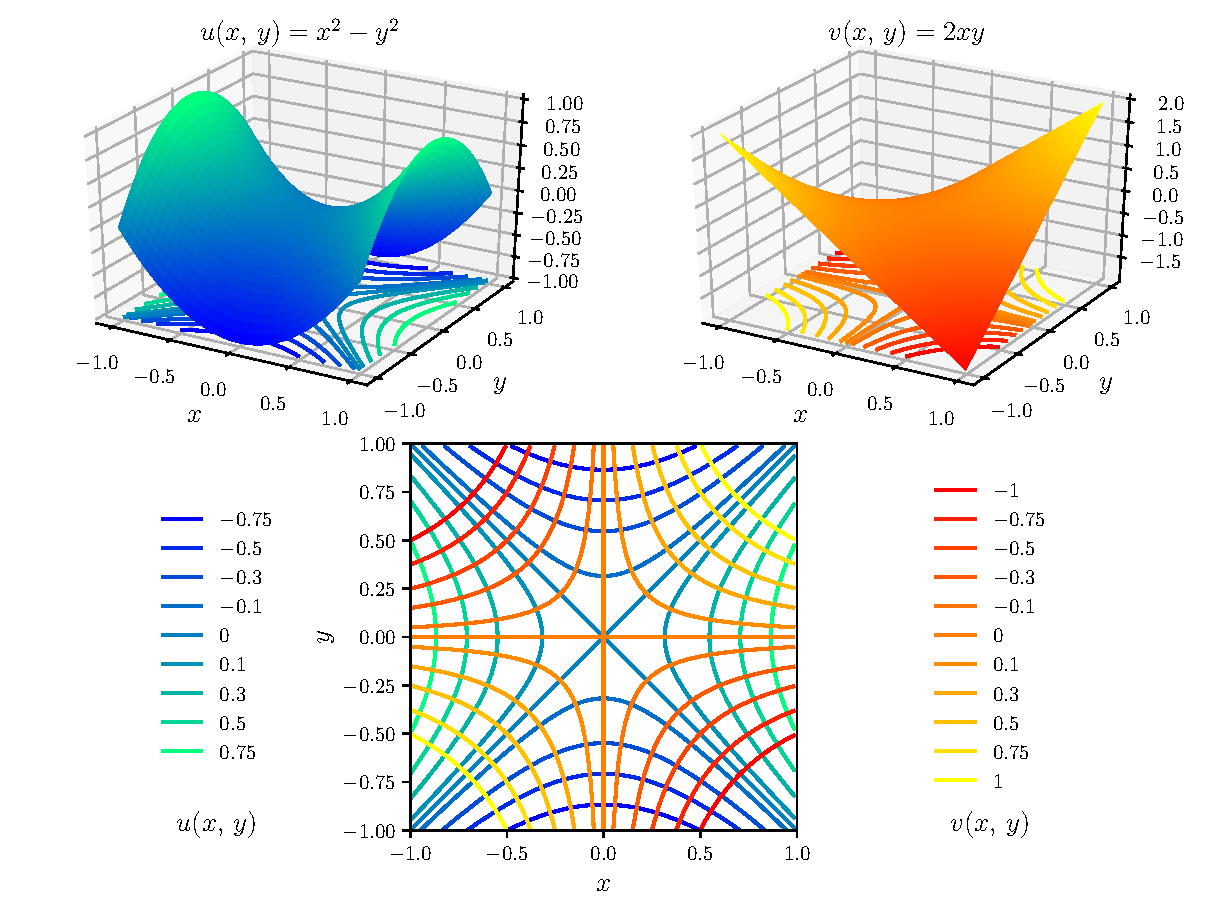
\includegraphics[width=\textwidth]{figuras/exercise_27_2_example.pdf}
 \caption{\label{fig:exercise_27_2_example} Superficie y curvas de nivel de las funciones componentes \(u(x,\,y)=x^2-y^2\) y \(v(x,\,y)=2xy\) de la función \(f(z)=z^2\). Las tangentes a las curvas de nivel de ambos componentes son perpendiculares en los puntos de intersección, excepto en el punto \((0,\,0)\), donde se cumple que \(f'(0)=0\).}
 \end{center}
\end{figure}

\subsubsection{Ejercicio 3}

Mostrar que cuando \(f(z)=z^2\), las curvas de nivel \(u(x,\,y)=c_1\) y \(v(x,\,y)=c_2\) de las funciones componentes son las hipérbolas indicadas en la figura \ref{fig:exercise_27_2_example}. Observar la ortogonalidad de las dos familias, descripta en el Ejercicio 2. Observar que las curvas \(u(x,\,y)=0\) y \(v(x,\,y)=0\) se intersectan en el origen pero no son ortogonales entre si. ¿Porque este hecho es acorde al resultado del Ejercicio 2? 

\paragraph{Solución} El hecho de que las curvas de nivel 
\[
 u(x,\,y)=x^2-y^2=c_1
 \qquad\qquad\textrm{y}\qquad\qquad
 v(x,\,y)=2xy=c_2
\]
de las funciones componentes de \(f(z)=z^2\) son las hipérbolas mostradas en la figura \ref{fig:exercise_27_2_example} se explicó en la sección \ref{sec:square_mapping}.

Como se explicó en el Ejercicio 2, las curvas de nivel \(u(x,\,y)=0\) y \(v(x,\,y)=0\) se intersectan en el origen pero no son ortogonales debido a que \(f'(0)=0\).

\subsubsection{Ejercicio 4}

Bosquejar las familias de curvas de nivel de las funciones componentes \(u\) y \(v\) cuando \(f(z)=1/z\) y notar la ortogonalidad descripta en el Ejercicio 2.

\paragraph{Solución} Como
\[
 f(z)=\frac{1}{z}=\frac{\overline{z}}{z\overline{z}}=\frac{\overline{z}}{|z|^2}=\frac{x-iy}{x^2+y^2},
\]
las funciones componentes son
\[
 u(x,\,y)=\frac{x}{x^2+y^2}
 \qquad\qquad\textrm{y}\qquad\qquad
 v(x,\,y)=-\frac{y}{x^2+y^2}.
\]
La ecuación de la curva de nivel 
\[
 u(x,\,y)=\frac{x}{x^2+y^2}=c_1
\]
se puede escribir como
\[
 x^2+y^2-\frac{x}{c_1}=0,
\]
y es equivalente a
\[
 x^2-2\left(\frac{1}{2c_1}\right)x+\left(\frac{1}{2c_1}\right)^2+y^2=\left(\frac{1}{2c_1}\right)^2
\]
o
\[
 \left(x-\frac{1}{2c_1}\right)^2+y^2=\left(\frac{1}{2c_1}\right)^2.
\]
Esto es la ecuación de una circunferencia de centro \([1/(2c_1),\,0]\) y radio \(1/(2c_1)\). Por lo tanto, las curvas de nivel del componente \(u\) son la familia de circunferencias con centro en el eje real \(y=0\) que pasan por el origen \((0,\,0)\), y se muestra en la figura \ref{fig:exercise_27_4}.
\begin{figure}[!htb]
 \begin{center}
 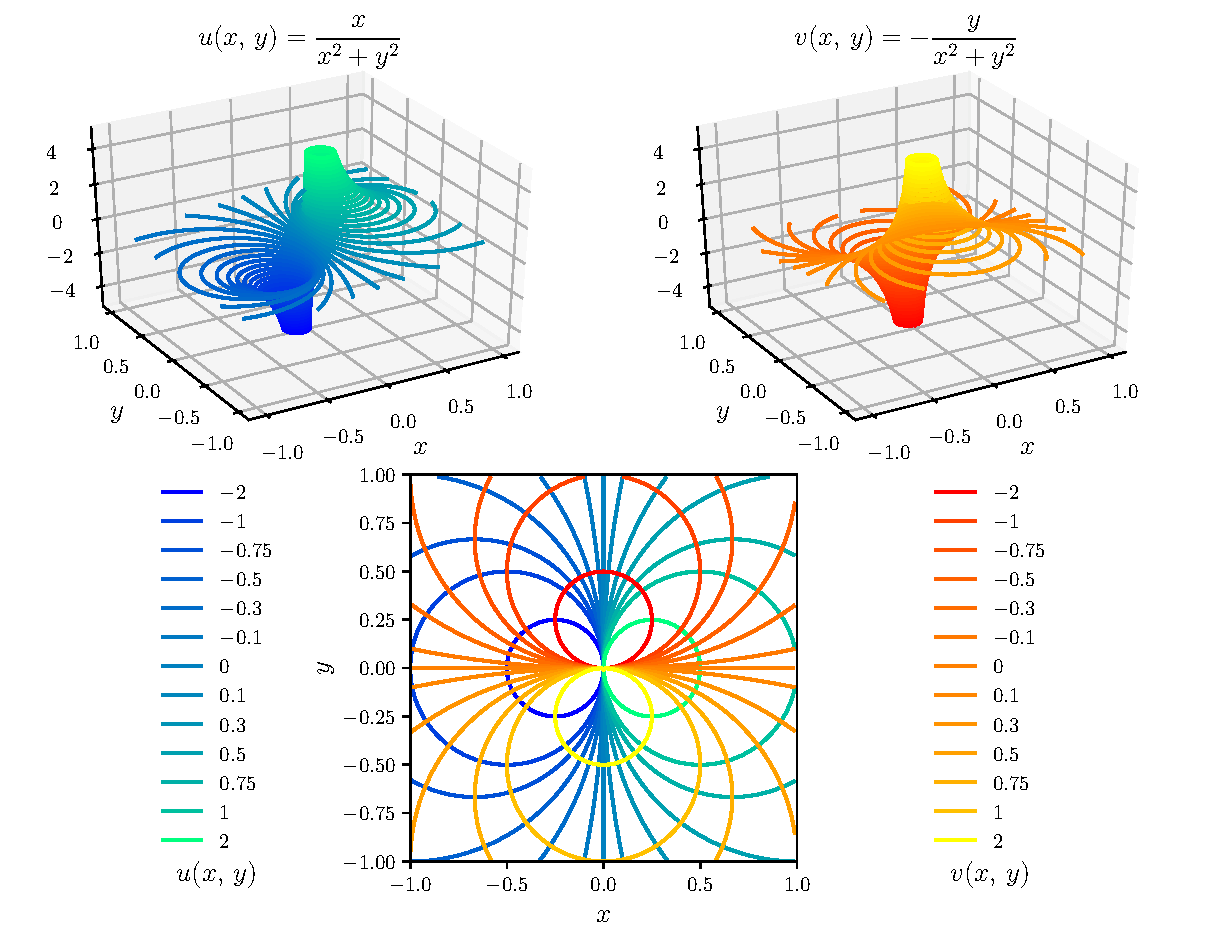
\includegraphics[width=\textwidth]{figuras/exercise_27_4.pdf}
 \caption{\label{fig:exercise_27_4} Superficie y curvas de nivel de las funciones componentes \(u(x,\,y)=x/(x^2+y^2)\) y \(v(x,\,y)=-y/(x^2+y^2)\) de la función \(f(z)=1/z\). Las curvas de nivel del componente \(u\) es la familia de circunferencias con centro en el eje real que pasan por el origen y las curvas de nivel del componente \(v\) es la familia de circunferencias con centro en el eje imaginario que pasan por el origen. Se observa que ambas familas son ortogonales.}
 \end{center}
\end{figure}

Realizando un razonamiento análogo, la ecuación de las curvas de nivel del componente \(v\) 
\[
 v(x,\,y)=-\frac{y}{x^2+y^2}=c_2
\]
es
\[
 x^2+\left(y+\frac{1}{2c_2}\right)^2=\left(\frac{1}{2c_2}\right)^2.
\]
Esto es la ecuación de una circunferencia de centro \([0,\,-1/(2c_2)]\) y radio \(1/(2c_2)\). Por lo tanto, las curvas de nivel del componente \(v\) son la familia de circunferencias con centro en el eje imaginario \(x=0\) que pasan por el origen \((0,\,0)\), como se muestra en la figura \ref{fig:exercise_27_4}. Como se aprecia en la figura, ambas familias de curvas son ortogonales.

\subsubsection{Ejercicio 5}

Hacer el Ejercicio 4 empleando coordenadas polares. 

\paragraph{Solución} Con \(z=re^{i\theta}\), la función se puede expresar como
\[
 f(z)=\frac{1}{z}=\frac{1}{re^{i\theta}}=\frac{e^{-i\theta}}{r}=\frac{\cos\theta}{r}-i\frac{\sen\theta}{r},
\]
resultando en que las funciones componentes en coordenadas polares son
\[
 u(r,\,\theta)=\frac{\cos\theta}{r}
 \qquad\qquad\textrm{y}\qquad\qquad
 v(r,\,\theta)=-\frac{\sen\theta}{r}.
\]
Para realizar el análisis de las curvas de nivel, se parte considerando que la ecuación de una circunferencia en coordenadas polares es\footnote{Ver \url{https://en.wikipedia.org/wiki/Circle\#Equations}, por ejemplo.}
\[
 r^2-2rr_0\cos(\theta-\varphi)+r_0^2=a^2,
\]
donde \(a\) es el radio, \((r_0,\,\varphi)\) son las coordenadas polares del centro y \((r,\,\theta)\) son las coordenadas polares de los puntos de la circunferencia. En el caso particular en que el origen pertenece a la circunferencia, se cumple que \(r_0=a\), y la ecuación se reduce a
\begin{equation}\label{eq:circunsference_equation_polar_origin}
 r=2r_0\cos(\theta-\varphi).
\end{equation}

Las ecuaciones de las curvas de nivel del componente \(u\) son
\[
 u(r,\,\theta)=\frac{\cos\theta}{r}=c_1,
\]
que se pueden escribir como
\[
 r=\frac{\cos\theta}{c_1}
 \qquad\qquad\textrm{o}\qquad\qquad
 r=\left\{ 
 \begin{array}{ll}
  2\left(\dfrac{1}{2c_1}\right)\cos\theta & c_1\geq0\\[\bigskipamount]
  -2\left(\dfrac{1}{2|c_1|}\right)\cos\theta=2\left(\dfrac{1}{2|c_1|}\right)\cos(\theta-\pi) & c_1<0
 \end{array}
 \right.,
\]
donde se empleó la identidad trigonométrica \(-\cos\theta=\cos(\theta-\pi)\).
Comparando este resultado con el de la ecuación \ref{eq:circunsference_equation_polar_origin}, se concluye que las curvas de nivel son circunferencias de radio \(1/(2|c_1|)\) y centro con coordenadas polares \([1/(2c_1),\,0]\) si \(c_1\geq0\) o \([1/(2|c_1|),\,\pi]\) si \(c_1<0\), es decir, la familia de circunferencias con centro en el eje real que pasan por el origen.

Las ecuaciones de las curvas de nivel del componente \(v\) son
\[
 v(r,\,\theta)=-\frac{\sen\theta}{r}=c_2,
\]
que se pueden escribir como
\[
 r=-\frac{\sen\theta}{c_2}
 \qquad\qquad\textrm{o}\qquad\qquad
 r=\left\{ 
 \begin{array}{ll}
  2\left(\dfrac{1}{2c_2}\right)\cos\left(\theta+\dfrac{\pi}{2}\right) & c_2\geq0\\[\bigskipamount]
  2\left(\dfrac{1}{2|c_2|}\right)\sen\theta=2\left(\dfrac{1}{2|c_2|}\right)\cos\left(\theta-\dfrac{\pi}{2}\right) & c_2<0
 \end{array}
 \right.
\]
donde se empleó la identidad trigonométrica \(\mp\sen\theta=\cos(\theta\pm\pi/2)\). Comparando este resultado con el de la ecuación \ref{eq:circunsference_equation_polar_origin}, se concluye que las curvas de nivel son circunferencias de radio \(1/(2|c_2|)\) y centro con coordenadas polares \([1/(2c_2),\,-\pi/2]\) si \(c_2\geq0\) o \([1/(2|c_2|),\,\pi/2]\) si \(c_2<0\), es decir, la familia de circunferencias con centro en el eje imaginario que pasan por el origen. Las curvas de nivel de ambos componentes se muestran en la figura \ref{fig:exercise_27_4}.

\subsubsection{Ejercicio 6}

Esbozar la familia de curvas de nivel de las funciones componentes \(u\) y \(v\) cuando 
\[
 f(z)=\frac{z-1}{z+1}
\]
y notar como se ilustra en este caso el resultado del Ejercicio 2.

\paragraph{Solución} Para calcular los componentes se observa que 
\[
 f(z)=\frac{z-1}{z+1}=\frac{(z-1)\overline{(z+1)}}{(z+1)\overline{(z+1)}}
  =\frac{(z-1)(\overline{z}+1)}{|z+1|^2}
  =\frac{z\overline{z}+z-\overline{z}-1}{|z+1|^2}
  =\frac{|z|^2+z-\overline{z}-1}{|z+1|^2}.
\]
Considerando que \(|z|^2=x^2+y^2\), \(|z+1|^2=(x+1)^2+y^2\) y \(z-\overline{z}=2iy\) se obtiene que 
\[
 f(z)=\frac{x^2+y^2-1+2iy}{(x+1)^2+y^2}
\]
por lo que los componentes son
\[
 u(x,\,y)=\frac{x^2+y^2-1}{(x+1)^2+y^2}
 \qquad\qquad\textrm{y}\qquad\qquad
 v(x,\,y)=\frac{2y}{(x+1)^2+y^2}.
\]

Las curvas de nivel del componente \(u\) están dadas por 
\[
 \frac{x^2+y^2-1}{(x+1)^2+y^2}=c_1
 \qquad\Leftrightarrow\qquad
 x^2+y^2-1=c_1[(x+1)^2+y^2]
 \qquad\Leftrightarrow\qquad
 x^2+y^2-1=c_1(x^2+2x+1+y^2)
\]
resultando en que 
\[
 x^2(c_1-1)+2c_1x+(c_1+1)+y^2(c_1-1)=0,
\]
es decir,
\begin{equation}\label{eq:exercise_26_07_u}
 x^2+\frac{2c_1x}{c_1-1}+\frac{c_1+1}{c_1-1}+y^2=0.
\end{equation}
Empleando la técnica de completar el cuadrado, considerando la identidad 
\[
 \left(x+\frac{c_1}{c_1-1}\right)^2=x^2+\frac{2c_1x}{c_1-1}+\frac{c_1^2}{(c_1-1)^2},
\]
la ecuación \ref{eq:exercise_26_07_u} queda 
\[
 \left(x+\frac{c_1}{c_1-1}\right)^2+y^2-\frac{c_1^2}{(c_1-1)^2}+\frac{c_1+1}{c_1-1}=0
\]
resultando en
\[
 \left(x+\frac{c_1}{c_1-1}\right)^2+y^2=\frac{1}{(c_1-1)^2}
\]
Esto es una circunferencia de centro \([-c_1/(c_1-1),\,0]\) y radio \(1/|c_1-1|\). Se observa además que el punto \((-1,\,0)\) pertenece a la circunferencia. Se concluye que las curvas de nivel del componente \(u\) es la familia de circunferencias con centro en el eje real que pasan por el punto \((-1,\,0)\) y se muestran en la figura \ref{fig:exercise_27_6}.
\begin{figure}[!htb]
 \begin{center}
 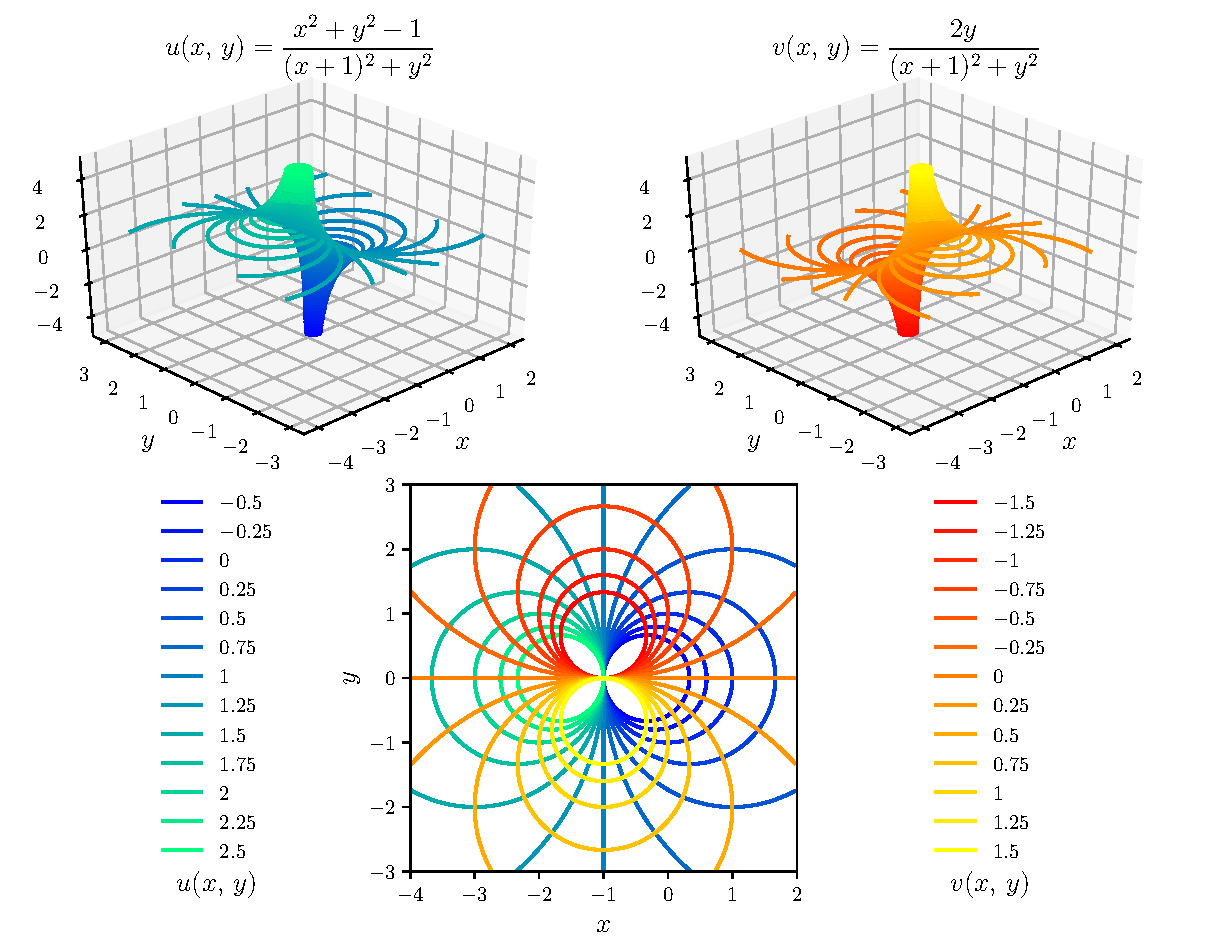
\includegraphics[width=\textwidth]{figuras/exercise_27_6.pdf}
 \caption{\label{fig:exercise_27_6} Superficie y curvas de nivel de las funciones componentes \(u(x,\,y)\) y \(v(x,\,y)\) de la función \(f(z)=(z-1)/(z+1)\). Las curvas de nivel del componente \(u\) es la familia de circunferencias con centro en el eje real que pasan por el punto \((-1,\,0)\) y las curvas de nivel del componente \(v\) es la familia de circunferencias con centro en la recta vertical \(x=-1\) que pasan por el punto \((-1,\,0)\). Se observa que ambas familas son ortogonales.}
 \end{center}
\end{figure}

Las curvas de nivel del componente \(v\) están dadas por 
\[
 \frac{2y}{(x+1)^2+y^2}=c_2,
\]
es decir,
\begin{equation}\label{eq:exercise_26_07_v}
 (x+1)^2+y^2-\frac{2y}{c_2}=0.
\end{equation}
Nuevamente, empleando la técnica de completar el cuadrado, como
\[
 \left(y-\frac{1}{c_2}\right)^2=y^2-\frac{2y}{c_2}+\frac{1}{c_2^2},
\]
la ecuación \ref{eq:exercise_26_07_v} se puede escribir como
\[
 (x+1)^2+\left(y-\frac{1}{c_2}\right)^2=\frac{1}{c_2^2}.
\]
Esto es una circunferencia de centro \((-1,\,1/c_2)\) y radio \(1/|c_2|\). Se observa además que el punto \((-1,\,0)\) pertenece a la circunferencia. Se concluye que las curvas de nivel del componente \(v\) es la familia de circunferencias con centro en la recta vertical \(x=-1\) que pasan por el punto \((-1,\,0)\) y se muestran en la figura \ref{fig:exercise_27_6}.

\section{Funciones analíticas determinadas unívocamente}\label{sec:uniquely_determined_analytic_functions}

En esta sección y la siguiente se estudia como los valores de una función analítica en un dominio \(D\) son afectados por sus valores en un subdominio de \(D\) o en un segmento de recta en \(D\). 

\paragraph{Lema.} Supóngase que 
\begin{enumerate}
 \item[(\textit{a})] una función \(f\) es analítica en un dominio \(D\);
 \item[(\textit{b})] \(f(z)=0\) en un dominio o segmento de recta contenido en \(D\)
\end{enumerate}
Entonces, se cumple que \(f(z)\equiv0\) en \(D\), es decir, \(f(z)\) es idénticamente nula en \(D\).

Supóngase ahora que dos funciones \(f\) y \(g\) son analíticas en el mismo dominio \(D\) y \(f(z)=g(z)\) en un dominio o segmento de recta contenido en \(D\). La diferencia
\[
 h(z)=f(z)-g(z)
\]
también es analítica en \(D\) y \(h(z)=0\) en el dominio o segmento. De acuerdo al lema, \(h(z)\equiv0\) en \(D\) y por lo tanto, \(f(z)=h(z)\) en cada punto de \(D\). Esto conduce al siguiente importante teorema.

\paragraph{Teorema.} Una función que es analítica en \(D\) está unívocamente determinada en \(D\) por los valores en un dominio o segmento de recta contenido en \(D\).

Este teorema es útil en el estudio de la extensión del dominio de definición de una función analítica. Mas precisamente, dados dos dominios \(D_1\) y \(D_2\), se considera la intersección \(D_1\cap D_2\). Si \(D_1\) y \(D_2\) tienen puntos en común y una función \(f_1\) es analítica en \(D_1\) \emph{puede} existir una función \(f_2\) analítica en \(D_2\) tal que \(f_2(z)=f_1(z)\) para cada \(z\) en la intersección \(D_1\cap D_2\). En ese caso \(f_2\) se llama \emph{continuación analítica} de \(f_1\) en el dominio \(D_2\).
\begin{figure}[!htb]
  \begin{minipage}[c]{0.4\textwidth}
    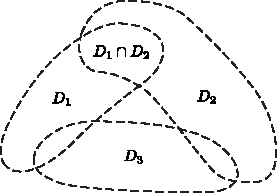
\includegraphics[width=\textwidth]{figuras/analytic_continuation.pdf}
  \end{minipage}\hfill
  \begin{minipage}[c]{0.5\textwidth}
    \caption{
       Continuación analítica.
    } \label{fig:analytic_continuation}
  \end{minipage}
\end{figure}

Si la continuación analítica existe, por el teorema anterior, es única. Es decir, no mas de una función puede ser analítica en \(D_2\) y asumir el valor \(f_1(z)\) en cada punto \(z\) del dominio \(D_1\cap D_2\) interior a \(D_2\). Sin embargo, si hay una continuación analítica \(f_3\) de \(f_2\) del dominio \(D_2\) al dominio \(D_3\) que intersecta al dominio \(D_1\), como se muestra en la figura \ref{fig:analytic_continuation}, no es necesariamente cierto que \(f_3(z)=f_1(z)\) para cada \(z\) en \(D_1\cap D_3\). Esto se ilustra en el Ejercicio 2 de la sección \ref{sec:reflection_principle}. Por la demostración de los teoremas en esta sección, recurrir a \cite{brown2013complex}.

Si \(f_2\) es la continuación analítica de \(f_1\) de un dominio \(D_1\) a un dominio \(D_2\), la función \(F\) definida como
\[
 F(z)=
 \left\{ 
 \begin{array}{ll}
  f_1(z) & \textrm{si }z\in D_1\\[\smallskipamount]
  f_2(z) & \textrm{si }z\in D_2,
 \end{array}
 \right.
\]
es analítica en la unión \(D_1\cup D_2\). La función \(F\) es la continuación analítica en \(D_1\cup D_2\) de \(f_1\) o \(f_2\), y \(f_1\) y \(f_2\) se dicen \emph{elementos} de \(F\).

\section{Principio de reflexión}\label{sec:reflection_principle}

El teorema en esta sección concierne al hecho de que algunas funciones analíticas tienen la propiedad de que \(\overline{f(z)}=f(\overline{z})\) en todos los puntos \(z\) de algunos dominios, mientras otras no. Se observa por ejemplo que las funciones \(z+1\) y \(z^2\) tienen esta propiedad cuando el dominio \(D\) es el plano complejo finito, pero lo mismo no es cierto para las funciones \(z+i\) y \(iz^2\). El siguiente teorema, denominado \emph{principio de reflexión} provee una forma de predecir cuando \(\overline{f(z)}=f(\overline{z})\). 

\paragraph{Teorema.} Supóngase que una función \(f\) es analítica en un dominio \(D\) que contiene un segmento del eje \(x\) y cuya mitad inferior es el reflejo de la mitad superior respecto al eje \(x\). Entonces 
\begin{equation}\label{eq:reflection_principle}
 \overline{f(z)}=f(\overline{z})
\end{equation}
para cada punto \(z\) en el dominio si y solo si \(f(x)\) es real para cada punto \(x\) en el segmento del eje real.

Se comienza la prueba asumiendo que \(f(x)\) es real en cada punto \(x\) del segmento. Se mostrará que 
\begin{equation}\label{eq:reflection_principle_proof_F}
 F(z)=\overline{f(\overline{z})}
\end{equation}
es analítica en \(D\), y se empleará ese resultado junto con la hipótesis para obtener \ref{eq:reflection_principle}. Para obtener la analiticidad de \(F(x)\) se escribe
\[
 f(z)=u(x,\,y)+iv(x,\,y)
 \qquad\qquad\textrm{y}\qquad\qquad
 F(z)=U(x,\,y)+iV(x,\,y).
\]
De esta forma,
\begin{equation}\label{eq:reflection_principle_f_reflected_components}
 \overline{f(\overline{z})}=u(x,\,-y)-iv(x,\,-y) 
\end{equation}
y por lo tanto, los componentes de \(F(z)\) y \(f(z)\) se relacionan por las ecuaciones
\[
 U(x,\,y)=u(x,\,-y)
 \qquad\qquad\textrm{y}\qquad\qquad
 V(x,\,y)=-v(x,\,-y).
\]
o, definiendo \(t=-y\),
\begin{equation}\label{eq:reflection_principle_proof_F_f_relation}
 U(x,\,y)=u(x,\,t)
 \qquad\qquad\textrm{y}\qquad\qquad
 V(x,\,y)=-v(x,\,t).
\end{equation}
Continuando, como por hipótesis \(f(x+it)\) es una función analítica de \(x+it\), las derivadas parciales de primer orden de las funciones componentes \(u(x,\,t)\) y \(v(x,\,t)\) son continuas en \(D\) y satisfacen las ecuaciones de Cauchy-Riemann, 
\begin{equation}\label{eq:reflection_principle_proof_cr_f}
 u_x=v_t
 \qquad\qquad\textrm{y}\qquad\qquad
 u_t=-v_x, 
\end{equation}
como se demostró en la sección \ref{sec:differentiability_sufficient_conditions}. Además, de las ecuaciones \ref{eq:reflection_principle_proof_F_f_relation},
\begin{equation}\label{eq:reflection_principle_proof_F_f_derivatives_1}
  U_x=u_x
 \qquad\qquad\textrm{y}\qquad\qquad
 V_y=\frac{\partial(-v)}{\partial t}\frac{dt}{dy}=(-v_t)(-1)=v_t,
\end{equation}
y de forma similar,
\begin{equation}\label{eq:reflection_principle_proof_F_f_derivatives_2}
 U_y=\frac{\partial u}{\partial t}\frac{dt}{dy}=(u_t)(-1)=-u_t
 \qquad\qquad\textrm{y}\qquad\qquad
 V_x=-v_x.
\end{equation}
Combinando las ecuaciones en \ref{eq:reflection_principle_proof_F_f_derivatives_1} con la primer ecuación en \ref{eq:reflection_principle_proof_cr_f} se obtiene que \(U_x=V_y\), y combinando las ecuaciones en \ref{eq:reflection_principle_proof_F_f_derivatives_2} con la segunda ecuación en \ref{eq:reflection_principle_proof_cr_f} se obtiene que \(U_y=-V_x\). Se obtuvo que las derivadas parciales de \(U(x,\,y)\) y \(V(x,\,y)\) satisfacen las ecuaciones de Cauchy-Riemann, y como esas derivadas son continuas, se concluye que \(F(z)\) es analítica en \(D\). Además, como \(f(x)\) es real en el segmento del eje real en \(D\), se cumple que \(v(x,\,0)=0\) en el segmento, y de las ecuaciones \ref{eq:reflection_principle_proof_F_f_relation}, se observa que 
\[
 F(x)=U(x,\,0)+iV(x,\,0)=u(x,\,0)-iv(x,\,0)=u(x,\,0)=f(x),
\]
es decir,
\begin{equation}\label{eq:reflection_principle_proof_conclution}
 F(z)=f(z)
\end{equation}
en cada punto del segmento. Por lo tanto, del teorema de la sección \ref{sec:uniquely_determined_analytic_functions} que indica que una función analítica definida en un dominio \(D\) queda determinada por unívocamente por los valores en cualquier segmento en \(D\) se concluye que la ecuación \ref{eq:reflection_principle_proof_conclution} es válida en todo el dominio \(D\). De la definición \ref{eq:reflection_principle_proof_F} de la función \(F(z)\) se obtiene que 
\begin{equation}\label{eq:reflection_principle_alt}
 \overline{f(\overline{z})}=f(z), 
\end{equation}
que es lo mismo que la ecuación \ref{eq:reflection_principle}, concluyendo la prueba.

Para probar el recíproco del teorema, se asume que se cumple la ecuación \ref{eq:reflection_principle}. De la ecuación \ref{eq:reflection_principle_f_reflected_components}, la forma \ref{eq:reflection_principle_alt} de la ecuación \ref{eq:reflection_principle} se puede escribir como 
\[
 u(x,\,-y)-iv(x,\,-y)=u(x,\,y)+iv(x,\,y)
\]
En particular, si \((x,\,0)\) es un punto del segmento del eje real en \(D\),
\[
 u(x,\,0)-iv(x,\,0)=u(x,\,0)+iv(x,\,0),
\]
e igualando las partes imaginarias, se obtiene que \(v(x,\,0)=0\). Se concluye que \(f(x)\) es real en el segmento del eje real en \(D\). 

\subsection*{Ejercicios}

\subsubsection{Ejercicio 1}

Emplear el teorema de la sección \ref{sec:uniquely_determined_analytic_functions} para mostrar que si  \(f(z)\) es analítica y no constante en un dominio \(D\), no puede ser constante en ningún entorno en \(D\).

\emph{Sugerencia:} suponer que \(f(z)\) tiene un valor constante \(w_0\) en algún entorno en \(D\).

\paragraph{Solución} \(f(z)\) es analítica en \(D\) y por absurdo, supóngase que \(f(z)=w_0\) constante en un entorno en \(D\). De esta forma, la función \(h(z)=f(z)-w_0\) es analítica en \(D\) y \(h(z)=0\) en dicho entorno en \(D\). Del lema de la sección \ref{sec:uniquely_determined_analytic_functions}, se debe  cumplir que \(h(z)=0\) en todo \(D\), o equivalentemente, \(f(z)=w_0\) constante en todo \(D\), contradiciendo la hipótesis. Se concluye que \(f(z)\) no puede ser constante en ningún entorno en \(D\).

\subsubsection{Ejercicio 2}

Comenzando con la función
\[
 f_1(z)=\sqrt{r}e^{i\theta/2}\qquad\textrm{con}\qquad r>0,\,0<\theta<\pi,
\]
y refiriéndose al ejemplo de la sección \ref{sec:cauchy_riemann_equations_polar} indicar porque
\[
 f_2(z)=\sqrt{r}e^{i\theta/2}\qquad\textrm{con}\qquad r>0,\,\frac{\pi}{2}<\theta<2\pi,
\]
es una continuación analítica de \(f_1\) al eje real negativo y el semiplano inferior. Luego, mostrar que la función 
\[
 f_3(z)=\sqrt{r}e^{i\theta/2}\qquad\textrm{con}\qquad r>0,\,\pi<\theta<\frac{5\pi}{2},
\]
es una continuación analítica de \(f_2\) al eje real positivo y al primer cuadrante, pero \(f_3(z)=-f_1(z)\) allí.

\paragraph{Solución} En el ejemplo de la sección \ref{sec:cauchy_riemann_equations_polar} se mostró que la función 
\[
 f(z)=\sqrt{r}e^{i\theta/2}\qquad\textrm{con}\qquad r>0,\,\alpha<\theta<\alpha+2\pi,
\]
es analítica en todo el dominio de definición. 

El dominio de definición \(D_1\) de la función \(f_1\) es el semiplano superior, y la función es analítica allí. Por otro lado, el dominio de definición \(D_2\) de la función \(f_2\) es el segundo cuadrante y el semiplano inferior, y es analítica allí. Se cumple entonces que 
\[
 D_1\cap D_2=\left\{r>0,\,\frac{\pi}{2}<\theta<\pi\right\}
\]
y además \(f_2(z)=f_1(z)\) para cada \(z\) en \(D_1\cap D_2\). Por lo tanto, \(f_2\) es la continuación analítica de \(f_1\) del semiplano superior al eje real negativo y el semiplano inferior.

De forma similar, el dominio \(D_3\) de la función \(f_3\) es el semiplano inferior y el primer cuadrante, y la función es analítica en todo el dominio. De esta forma, se cumple que 
\[
 D_2\cap D_3=\left\{r>0,\,\pi<\theta<2\pi\right\}
\]
y además, como \(f_3(z)=f_2(z)\) para cada \(z\) en \(D_2\cap D_3\), \(f_3\) es la continuación analítica de \(f_2\) al eje real positivo y al primer cuadrante.

Finalmente, se observa que los dominios \(D_1\) y \(D_3\) contienen al primer cuadrante. Efectivamente, en el dominio \(D_1\) los puntos del primer cuadrante se obtienen con \(0<\theta<\pi/2\), y en el dominio \(D_3\) los puntos del primer cuadrante se obtienen con \(2\pi<\theta<5\pi/4=2\pi+\pi/2\). Sea el punto \(z=re^{i\theta}\) con \(0<\theta<\pi/2\) y sea el punto \(z'=re^{i\theta'}\) con \(\theta'=\theta+2\pi\). De esta forma, \(z\in D_1\), \(z'\in D_3\) y además \(z'=z\), ya que
\[
 z'=re^{i\theta'}=re^{i(\theta+2\pi)}=re^{i\theta}e^{i2\pi}=re^{i\theta}=z.
\]
Se cumple que 
\[
 f_1(z)=\sqrt{r}e^{i\theta/2},
\]
y
\[
 f_3(z)=f_3(z')=\sqrt{r}e^{i\theta'/2}=\sqrt{r}e^{i(\theta+2\pi)/2}=\sqrt{r}e^{i\theta/2}e^{i\pi}=\sqrt{r}e^{i\theta/2}(-1)=-f_1(z).
\]
Se concluye que \(f_2\) es la continuación analítica de \(f_1\), \(f_3\) es la continuación analítica de \(f_2\) pero \(f_3\) no es la continuación analítica de \(f_1\) en \(D_1\cap D_3\).

\subsubsection{Ejercicio 3}

Indicar porque la función 
\[
 f_4(z)=\sqrt{r}e^{i\theta/2}\qquad\textrm{con}\qquad r>0,\,-\pi<\theta<\pi,
\]
es la continuación analítica de \(f_1\) del Ejercicio 2 al eje real positivo y el semiplano inferior.

\paragraph{Solución} El dominio de definición \(D_1\) de la función \(f_1\) es el semiplano superior, y la función es analítica allí. Por otro lado, el dominio de definición \(D_4\) de la función \(f_4\) es todo el plano excepto el eje real negativo, y es analítica allí. Se cumple entonces que 
\[
 D_1\cap D_4=\left\{r>0,\,0<\theta<\pi\right\}
\]
y además \(f_4(z)=f_1(z)\) para cada \(z\) en \(D_1\cap D_4\). Por lo tanto, \(f_4\) es la continuación analítica de \(f_1\) del semiplano superior al semiplano inferior y al eje real positivo.

\subsubsection{Ejercicio 4}

Del ejemplo de la sección \ref{sec:differentiability_sufficient_conditions} se sabe que la función 
\[
 f(z)=e^z=e^x\cos y+ie^x\sen y
\]
es diferenciable en todos lados en el plano complejo finito. Indicar como surge del principio de reflexión que 
\[
 \overline{f(z)}=f(\overline{z})
\]
para todo \(z\). Luego, verificarlo directamente.

\paragraph{Solución} Como el dominio de la función es todo el plano complejo, contiene todo el eje real, y la mitad inferior, que es todo el semiplano inferior, es el reflejo de la mitad superior, que es todo el semiplano superior. De esta forma el dominio cumple las condiciones del principio de reflexión. Como para un punto \(z=x+i0\) del eje real, la función toma el valor
\[
 f(z)=f(x)=e^x
\]
real, por el teorema de reflexión se cumple que \(\overline{f(z)}=f(\overline{z})\) para todo \(z\).

Para verificar el resultado de forma directa, se observa que 
\[
 \overline{f(z)}=e^x\cos y-ie^x\sen y,
\]
y además, con \(\overline{z}=x-iy\),
\[
 f(\overline{z})=e^x\cos(-y)+ie^x\sen(-y)=e^x\cos y-ie^x\sen y,
\]
resultando en que \(\overline{f(z)}=f(\overline{z})\) para todo \(z\).

\subsubsection{Ejercicio 5}

Mostrar que si la condición de que \(f(x)\) es real en el principio de reflexión se reemplaza por la condición de que \(f(x)\) es imaginario puro, la ecuación \ref{eq:reflection_principle} del principio cambia a 
\begin{equation}\label{reflection_principle_imaginary}
 \overline{f(z)}=-f(\overline{z}).
\end{equation}

\paragraph{Solución} Como se demostró en el teorema del principio de reflexión en la sección \ref{sec:reflection_principle}, la función
\begin{equation}\label{eq:exercise_26_05_F}
 F(z)=\overline{f(\overline{z})}
\end{equation}
es analítica en el dominio de definición \(D\) de \(f\). Para demostrar el teorema directo, supóngase que \(f(x)\) es imaginario puro en el segmento del eje real en \(D\). De esta forma, el componente real de \(f(z)\) es nulo en los puntos del segmento del eje real, es decir, \(u(x,\,0)=0\). Por lo tanto, de la ecuación \ref{eq:reflection_principle_proof_F_f_relation} en el teorema,
\[
 F(x)=U(x,\,0)+iV(x,\,0)=u(x,\,0)-iv(x,\,0)=-iv(x,\,0)=-f(x),
\]
es decir,
\begin{equation}\label{eq:exercise_26_05_F_f}
 F(z)=-f(z)
\end{equation}
en cada punto del segmento. Por lo tanto, del teorema de la sección \ref{sec:uniquely_determined_analytic_functions} que indica que una función analítica definida en un dominio \(D\) queda determinada por unívocamente por los valores en cualquier segmento en \(D\) se concluye que la ecuación \ref{eq:exercise_26_05_F_f} es válida en todo el dominio \(D\). De la definición \ref{eq:exercise_26_05_F} de la función \(F(z)\) se obtiene que
\begin{equation}\label{reflection_principle_imaginary_alt}
 \overline{f(\overline{z})}=-f(z), 
\end{equation}
que es lo mismo que la ecuación \ref{reflection_principle_imaginary}.

Para demostrar el recíproco, se asume que se cumple la ecuación \ref{reflection_principle_imaginary}, que se puede expresar como
\[
 u(x,\,y)-iv(x,\,y)=-u(x,\,-y)-iv(x,\,-y).
\]
En particular, si \((x,\,0)\) es un punto del segmento del eje real en \(D\),
\[
 u(x,\,0)-iv(x,\,0)=-u(x,\,0)-iv(x,\,0),
\]
e igualando las partes reales, se obtiene que \(u(x,\,0)=0\). Se concluye que \(f(x)\) es imaginario puro en el segmento del eje real en \(D\).

\chapter{Funciones elementales}

En este capítulo se consideran varias funciones elementales estudiadas en cálculo y se definen las  correspondientes funciones de variable compleja. Específicamente, se definen funciones analíticas de una variable compleja \(z\) que se reduce a una función elemental en cálculo cuando \(z=x+i0\).

\section{La función exponencial}\label{sec:exponential_function}

La función exponencial se define como
\[
 e^z=e^xe^{iy}=e^x(\cos y+i\sen y),\qquad\qquad\textrm{con}\qquad\qquad z=x+iy.
\]
Se observa que \(e^z\) se reduce a la función exponencial usual de cálculo cuando \(y=0\).

Hay varias propiedades que se extienden de \(e^x\) a \(e^z\). Algunas de ellas son las siguientes (ver la sección 30 de \cite{brown2013complex}):
\begin{itemize}
 \item \(e^z\neq0\) para todo \(z\).
 \item \(e^{z_1}e^{z_2}=e^{z_1+z_2}\)
 \item \(\dfrac{e^{z_1}}{e^{z_2}}=e^{z_1-z_2}\)
 \item \(\dfrac{d}{dz}e^z=e^z\) en todo el plano complejo. Esto se mostró en el ejemplo de la sección \ref{sec:differentiability_sufficient_conditions}.
\end{itemize}

Por otro lado, algunas propiedades de \(e^z\) no son esperadas. Por ejemplo, como
\[
 e^{z+2\pi i}=e^{z}e^{2\pi i}
  \qquad\qquad\textrm{y}\qquad\qquad
 e^{2\pi i}=1, 
\]
se encuentra que \(e^z\) es \emph{periódica} con período imaginario puro de \(2\pi i\):
\[
 e^{z+2\pi i}=e^{z}.
\]
Otra propiedad de \(e^z\) que no se traslada de \(e^x\) es que si bien \(e^x\) es siempre positivo, \(e^z\) puede ser negativo. Por ejemplo, \(e^{i\pi}=-1\), o mas en general,
\[
 e^{i(2n+1)\pi}=-1,\qquad\textrm{para}\qquad n=0,\,\pm1,\,\pm2,\,\dots.
\]
De hecho, \(e^z\) puede tomar el valor de cualquier número complejo no nulo.

\subsection*{Ejercicios}

\subsubsection{Ejercicio 1}

Mostrar que 
\[
 (\textit{a})\;\exp(2\pm3\pi i)=-e^2;\qquad\qquad 
 (\textit{b})\;\exp\left(\frac{2+\pi i}{4}\right)=\sqrt{\frac{e}{2}}(1+i);\qquad\qquad
 (\textit{c})\;\exp(z+\pi i)=-\exp z.
\]

\paragraph{Solución} 

\begin{enumerate}
 \item[(\textit{a})] \(\exp(2\pm3\pi i)=e^2e^{\pm3\pi i}=e^2(-1)=-e^2\).
 \item[(\textit{b})] \(\displaystyle\exp\left(\frac{2+\pi i}{4}\right)=\exp\left(\frac{1}{2}\right)\exp\left(\frac{\pi i}{4}\right)=\sqrt{e}\left(\cos\frac{\pi}{4}+i\sen\frac{\pi}{4}\right)=\sqrt{e}\left(\frac{1}{\sqrt{2}}+i\frac{1}{\sqrt{2}}\right)\sqrt{e}(1+i)\).
 \item[(\textit{c})] \(\exp(z+\pi i)=e^ze^{\pi i}=e^z(-1)=-e^z\).
\end{enumerate}

\subsubsection{Ejercicio 2}

Explicar porque la función \(f(z)=2z^2-3-ze^z+e^{-z}\) es completa.

\paragraph{Solución} \(2z^2-3\) es completa por ser un polinomio, \(ze^z\) es completa por ser el producto de funciones completas y \(e^{-z}=1/e^z\) es completa por ser el cociente de funciones completas y el denominador cumple que \(e^z\neq 0\) para todo \(z\). Se concluye que \(f(z)\) es completa por ser la suma de funciones completas.

\subsubsection{Ejercicio 3}

Emplear las ecuaciones de Cauchy-Riemann y el teorema de la sección \ref{sec:cauchy_riemann_equations} para mostrar que la función \(f(z)=e^{\overline{z}}\) no es analítica en ningún lado.

\paragraph{Solución} El hecho de que 
\[
 f(z)=e^{\overline{z}}=e^{x-iy}=e^xe^{-iy}
\]
no es analítica en ningún punto se mostró en el ejercicio 1 parte \((d)\) de la sección \ref{sec:cauchy_riemann_equations_polar}.

\subsubsection{Ejercicio 4}

Mostrar de dos formas que la función \(f(z)=\exp(z^2)\) es completa. ¿Cuál es su derivada?

\paragraph{Solución} Una forma de mostrar que la función 
\[
 f(z)=\exp(z^2)
\]
es completa es considerar que se trata de la composición \(f(z)=g[h(z)]\) de las funciones \(g(z)=e^z\) y \(h(z)=z^2\). Como las funciones \(g\) y \(h\) son completas, la composición \(f(z)=g[h(z)]\) es completa, como se justificó en el ejercicio 3 de la sección \ref{sec:analytic_functions}. Además, por la regla de la cadena, la derivada es
\[
 \frac{d}{dz}g[h(z)]=g'[h(z)]h'(z).
\]
Como en este caso
\[
 g'(z)=e^z
 \qquad\qquad\textrm{y}\qquad\qquad
 h'(z)=2z,
\]
la derivada queda
\[
 f'(z)=e^{z^2}(2z)=2ze^{z^2}.
\]

Una segunda forma de demostrar que la función es completa es empleando el teorema de la sección \ref{sec:differentiability_sufficient_conditions}. Para hacerlo, se parte calculando las funciones componentes. Como
\[
 f(z)=e^{z^2}=e^{x^2-y^2+2ixy}=e^{x^2-y^2}e^{2ixy}=e^{x^2-y^2}(\cos2xy+i\sen2xy),
\]
las funciones componente son
\[
 u(x,\,y)=e^{x^2-y^2}\cos2xy
 \qquad\qquad\textrm{y}\qquad\qquad
 v(x,\,y)=e^{x^2-y^2}\sen2xy.
\]
Para verificar si se cumplen las ecuaciones de Cauchy-Riemann, se calculan las derivadas parciales,
\[
 u_x=2xe^{x^2-y^2}\cos2xy+e^{x^2-y^2}(2y)(-\sen2xy)=2e^{x^2-y^2}(x\cos2xy-y\sen2xy)
\]
\[
 v_y=-2ye^{x^2-y^2}\sen2xy+e^{x^2-y^2}(2x)\cos2xy=2e^{x^2-y^2}(x\cos2xy-y\sen2xy).
\]
Como \(u_x=v_y\), se concluye que se cumple la primera ecuación de Cauchy-Riemann. Además,
\[
 u_y=-2ye^{x^2-y^2}\cos2xy+e^{x^2-y^2}(2x)(-\sen2xy)=-2e^{x^2-y^2}(y\cos2xy+x\sen2xy)
\]
\[
 v_x=2xe^{x^2-y^2}\sen2xy+e^{x^2-y^2}(2y)\cos2xy=2e^{x^2-y^2}(y\cos2xy+x\sen2xy),
\]
concluyendo que la segunda ecuación de Cauchy-Riemann \(u_y=-v_x\) también se cumple. Como las derivadas parciales existen y son continuas en todo el plano y las ecuaciones de Cauchy-Riemann se cumplen en todo el plano, se concluye que la función \(f\) es completa. Finalmente, la derivada es
\begin{align*}
 f'(z)&=u_x+iv_x\\
  &=2e^{x^2-y^2}\left[(x\cos2xy-y\sen2xy)+i(y\cos2xy+x\sen2xy)\right]\\
  &=2e^{x^2-y^2}\left[(x+iy)\cos2xy+(ix-y)\sen2xy\right]\\
  &=2e^{x^2-y^2}\left[(x+iy)\cos2xy+i(x+iy)\sen2xy\right]\\
  &=2(x+iy)e^{x^2-y^2}(\cos2xy+i\sen2xy)\\
  &=2(x+iy)e^{x^2-y^2}e^{2ixy}\\
  &=2(x+iy)e^{x^2-y^2+2ixy}\\
  &=2(x+iy)e^{(x+iy)^2},
\end{align*}
resultando en que
\[
 f'(z)=2ze^{z^2}.
\]

\subsubsection{Ejercicio 5}

Escribir \(|e^{2z+i}|\) y \(|e^{iz^2}|\) en términos de \(x\) y \(y\). Luego mostrar que 
\[
 |e^{2z+i}+e^{iz^2}|\leq e^{2x}+e^{-2xy}.
\]

\paragraph{Solución} Por un lado se ve que 
\[
 e^{2z+i}=e^{2(x+iy)+i}=e^{2x}e^{i(2y+1)},
\]
y por lo tanto
\[
 |e^{2z+i}|=|e^{2x}||e^{i(2y+1)}|=|e^{2x}|=e^{2x},
\]
donde se consideró que si \(x\) es un número real, se cumple que \(|e^{ix}|=1\) y \(e^x>0\). Por otro lado se tiene que 
\[
 e^{iz^2}=e^{i(x^2-y^2+2ixy)}=e^{-2xy}e^{i(x^2-y^2)}
\]
y por lo tanto
\[
 |e^{iz^2}|=|e^{-2xy}||e^{i(x^2-y^2)}|=|e^{-2xy}|=e^{-2xy}.
\]
Luego,
\[
 |e^{2z+i}+e^{iz^2}|\leq|e^{2z+i}|+|e^{iz^2}|=e^{2x}+e^{-2xy},
\]
donde se empleó la desigualdad triangular y los resultados obtenidos previamente.

\subsubsection{Ejercicio 6}

Mostrar que \(|e^{z^2}|\leq e^{|z|^2}\).

\paragraph{Solución} Por un lado se ve que 
\[
 e^{z^2}=e^{x^2-y^2+2ixy}=e^{x^2-y^2}e^{2ixy}
\]
y por lo tanto,
\[
 |e^{z^2}|=|e^{x^2-y^2}||e^{2ixy}|=|e^{x^2-y^2}|=e^{x^2-y^2}.
\]
Además,
\[
 e^{|z|^2}=e^{x^2+y^2}
\]
Como \(x^2-y^2\leq x^2+y^2\) y la función exponencial real es creciente, se cumple que 
\[
 e^{x^2-y^2}\leq e^{x^2+y^2},
\]
concluyendo que 
\[
 |e^{z^2}|\leq e^{|z|^2}.
\]

\subsubsection{Ejercicio 7}

Probar que \(|e^{-2z}|<1\) si y solo si \(\Re z>0\).

\paragraph{Solución} Se observa que
\[
 |e^{-2z}|=|e^{-2(x+iy)}|=|e^{-2x}e^{-2iy}|=|e^{-2x}||e^{-2iy}|=|e^{-2x}|=e^{-2x}.
\]
Como \(e^{-2x}\geq1\) si \(x\leq0\) y \(e^{-2x}<1\) si \(x>0\), y además \(x=\Re z\), se cumple que \(|e^{-2z}|<1\) si y solo si \(\Re z>0\). 

\subsubsection{Ejercicio 8}

Encontrar todos los valores de \(z\) tal que 
\[
 (\textit{a})\;\exp z=-2;\qquad\qquad 
 (\textit{b})\;\exp z=1+i;\qquad\qquad
 (\textit{c})\;\exp(2z-1)=1.
\]

\paragraph{Solución} 

\begin{enumerate}
 \item[(\textit{a})] 
 \[
  e^z=-2
  \qquad\qquad\Leftrightarrow\qquad\qquad
  e^xe^{iy}=2e^{i(2n+1)\pi},
  \qquad\qquad\textrm{con }n=0,\,\pm1,\,\pm2,\,\dots.
 \]
 Por lo tanto, igualando el módulo y la fase, se tiene que 
 \[
  \begin{array}{l}
   e^x=2\\
   y=(2n+1)\pi
  \end{array}
  \qquad\qquad\Rightarrow\qquad\qquad
  \begin{array}{l}
   x=\ln 2\\
   y=(2n+1)\pi
  \end{array}
  \qquad\qquad\Rightarrow\qquad\qquad
  z=\ln2+i(2n+1)\pi.
 \]
 \item[(\textit{b})] 
 \[
  e^z=1+i
  \qquad\qquad\Leftrightarrow\qquad\qquad
  e^xe^{iy}=\sqrt{2}\exp\left[i\left(\frac{\pi}{4}+2n\pi\right)\right],
  \qquad\qquad\textrm{con }n=0,\,\pm1,\,\pm2,\,\dots.
 \]
 Por lo tanto, igualando el módulo y la fase, se tiene que 
 \[
  \begin{array}{l}
   e^x=\sqrt{2}\\[\medskipamount]
   y=\dfrac{\pi}{4}+2n\pi
  \end{array}
  \qquad\Rightarrow\qquad
  \begin{array}{l}
   x=\dfrac{1}{2}\ln 2\\[\medskipamount]
   y=\left(2n+\dfrac{1}{4}\right)\pi
  \end{array}
  \qquad\Rightarrow\qquad
  z=\frac{1}{2}\ln2+i\left(2n+\dfrac{1}{4}\right)\pi.
 \]
 \item[(\textit{c})] 
 \[
  e^{2z-1}=1
  \qquad\qquad\Leftrightarrow\qquad\qquad
  e^{2x-1}e^{2iy}=e^{i2n\pi},
  \qquad\qquad\textrm{con }n=0,\,\pm1,\,\pm2,\,\dots.
 \]
 Por lo tanto, igualando el módulo y la fase, se tiene que 
 \[
  \begin{array}{l}
   e^{2x-1}=1\\[\medskipamount]
   2y=2n\pi
  \end{array}
  \qquad\Rightarrow\qquad
  \begin{array}{l}
   2x-1=0\\[\medskipamount]
   y=n\pi
  \end{array}
  \qquad\Rightarrow\qquad
  z=\frac{1}{2}+in\pi.
 \]
\end{enumerate}

\subsubsection{Ejercicio 9}

Mostrar que \(\overline{e^{iz}}=e^{i\overline{z}}\) si y solo si \(z=n\pi\) con \(n=0,\,\pm1,\,\pm2,\,\dots\). Comparar con el ejercicio 4 de la sección \ref{sec:reflection_principle}.

\paragraph{Solución} Se observa que 
\[
 \overline{e^{iz}}=\overline{e^{i(x+iy)}}=\overline{e^{-y+ix}}=\overline{e^{-y}e^{ix}}=
 (\overline{e^{-y}})(\overline{e^{ix}})\overset{(a)}{=}e^{-y}e^{-ix}=e^{-y-ix}=e^{-i(x-iy)}=e^{-i\overline{z}}, 
\]
donde en \((a)\) se consideró que \(\overline{e^{ix}}=e^{-ix}\), que es cierto porque \(e^{ix}\) es un número complejo de argumento \(x\), por lo que su conjugado tiene argumento \(-x\). Se obtuvo que 
\[
 \overline{e^{iz}}=e^{-i\overline{z}}.
\]
Por lo tanto,
\[
 \overline{e^{iz}}=e^{i\overline{z}}
 \qquad\Leftrightarrow\qquad
 e^{-i\overline{z}}=e^{i\overline{z}}
 \qquad\Leftrightarrow\qquad
 e^{2i\overline{z}}=1
 \qquad\Leftrightarrow\qquad
 e^{2i\overline{z}}=e^{i2n\pi}.
\]
Se concluye que \(\overline{e^{iz}}=e^{i\overline{z}}\) si y solo si
\[
 \overline{z}=n\pi
 \qquad\qquad\Leftrightarrow\qquad\qquad
 x-iy=n\pi+i0,
\]
es decir \(x=n\pi\) y \(y=0\).

Para comparar el resultado con el resultado del ejercicio 4 de la sección \ref{sec:reflection_principle}, se considera la función
\[
 f(z)=e^{iz},
\]
y se verá en que puntos del plano es analítica. Para hacerlo, se parte calculando los componentes. Como
 \[
  f(z)=e^{iz}=e^{i(x+iy)}=e^{-y}e^{ix}=e^{-y}(\cos x+i\sen x)
 \]
 los componentes son 
 \[
  u=e^{-y}\cos x
  \qquad\qquad\textrm{y}\qquad\qquad
  v=e^{-y}\sen x
 \]
 y las derivadas parciales son
 \[
 \begin{array}{ll}
  u_x=-e^{-y}\sen x\qquad\qquad\qquad\qquad&u_y=-e^{-y}\cos x\\[\smallskipamount]
  v_y=-e^{-y}\sen x\qquad\qquad\qquad\qquad&v_x=e^{-y}\cos x.
 \end{array}
 \]
 Se observa que las derivadas parciales son continuas y cumplen las ecuaciones de Cauchy-Riemann \(u_x=v_y\) y \(u_y=-v_x\) en todo el plano complejo, por lo que \(f(z)\) es analítica en todo el plano complejo (ver la sección \ref{sec:differentiability_sufficient_conditions}). Sin embargo, se observa que en el eje real \(z=x+i0\),
 \[
  f(x)=e^{ix}=\cos x+i\sen x
 \]
 no es real, y por lo tanto no se cumplen las condiciones del teorema de reflexión de la sección \ref{sec:reflection_principle}, concluyendo que no se cumple que \(\overline{f(z)}=f(\overline{z})\) en todo el plano complejo, acorde al resultado obtenido antes. En el caso de la función \(f(z)=e^z\) de ejercicio 4 de la sección \ref{sec:reflection_principle}, se cumplen las condiciones del principio de reflexión y por lo tanto \(\overline{f(z)}=f(\overline{z})\).

\subsubsection{Ejercicio 10}

\begin{enumerate}
 \item[(\textit{a})] Mostrar que si \(e^z\) es real, \(\Im z=n\pi\), con \(n=0,\,\pm1,\,\pm2,\,\dots\).
 \item[(\textit{b})] Si \(e^z\) es imaginario puro, ¿qué restricción cumple \(z\)?
\end{enumerate}

\paragraph{Solución} Como
\[
 e^{z}=e^x\cos y+ie^x\sen x,
\]
los componentes son
\[
 u(x,\,y)=e^x\cos y
 \qquad\qquad\textrm{y}\qquad\qquad
 v(x,\,y)=e^x\sen y.
\]
\begin{enumerate}
 \item[(\textit{a})] Si \(e^z\) es real,
 \[
  v(x,\,y)=e^x\sen y=0
  \qquad\qquad\Leftrightarrow\qquad\qquad
  \sen y=0
  \qquad\qquad\Leftrightarrow\qquad\qquad
  y=n\pi.
 \]
 Como \(y=\Im z\), se concluye que si \(e^z\) es real, \(\Im z=n\pi\), con \(n=0,\,\pm1,\,\pm2,\,\dots\).
 \item[(\textit{b})] Si \(e^z\) es imaginario puro,
  \[
  u(x,\,y)=e^x\cos y=0
  \qquad\qquad\Leftrightarrow\qquad\qquad
  \cos y=0
  \qquad\qquad\Leftrightarrow\qquad\qquad
  y=\frac{\pi}{2}+2n\pi.
 \]
 Se concluye que si \(e^z\) es imaginario puro,
 \[
  \Im z=\frac{\pi}{2}+2n\pi=\left(\frac{1}{2}+2n\right)\pi
  \qquad\qquad\textrm{con}\qquad\qquad
  n=0,\,\pm1,\,\pm2,\,\dots.
 \]
\end{enumerate}

\subsubsection{Ejercicio 11}

Describir el comportamiento de \(e^z=e^xe^{iy}\) cuando \((a)\) \(x\) tiende a \(-\infty\); \((b)\) \(y\) tiende a \(\infty\).

\paragraph{Solución}

\begin{enumerate}
 \item[(\textit{a})] \(\displaystyle\lim_{x\to\-\infty}e^xe^{iy}=0\).
 \item[(\textit{b})] Cuando \(y\) tiende a \(\infty\), \(e^xe^{iy}\) se mueve en el círculo de radio \(e^x\) constante en sentido antihorario.
\end{enumerate}

\subsubsection{Ejercicio 12}

Escribir \(\Re(e^{1/z})\) en términos de \(x\) y \(y\). ¿Porqué esta función es armónica en todo dominio que no contenga al origen?

\paragraph{Solución} Como
\[
 \exp\left(\frac{1}{z}\right)=\exp\left(\frac{\overline{z}}{|z|^2}\right)
 =\exp\left(\frac{x-iy}{x^2+y^2}\right)
 =\exp\left(\frac{x}{x^2+y^2}\right)\left[\cos\left(\frac{y}{x^2+y^2}\right)+i\sen\left(\frac{y}{x^2+y^2}\right)\right],
\]
se tiene que 
\[
 \Re(e^{1/z})=\exp\left(\frac{x}{x^2+y^2}\right)\cos\left(\frac{y}{x^2+y^2}\right).
\]

Como \(e^{1/z}\) es la composición de las funciones \(e^z\) con \(1/z\) y \(e^z\) es analítica en todo el plano y \(1/z\) es analítica en todo el plano excepto el origen, \(e^{1/z}\) es analítica en todo el plano excepto el origen. Por lo tanto, del teorema de la sección \ref{sec:harmonic_functions}, se cumple que \(u(x,\,y)=\Re(e^{1/z})\) es armónica en todo dominio que no contenga al origen.

\subsubsection{Ejercicio 13}

Sea la función \(f(x,\,y)=u(x,\,y)+iv(x,\,y)\) armónica en un dominio \(D\). Justificar porqué las funciones
\[
 U(x,\,y)=e^{u(x,\,y)}\cos v(x,\,y)
 \qquad\qquad\textrm{y}\qquad\qquad
 V(x,\,y)=e^{u(x,\,y)}\sen v(x,\,y)
\]
son armónicas en \(D\).

\paragraph{Solución} Como \(e^z\) es anaítica en todo el plano complejo y \(f(z)\) es analítica en \(D\), la composición \(e^{f(z)}\) es analítica en \(D\). De esta forma,
\[
 e^{f(z)}=e^ue^{iv}=e^u(\cos v+i\sen v),
\]
es analítica en \(D\), y por el teorema de la sección \ref{sec:harmonic_functions}, sus componentes
\[
 U=e^u\cos v
 \qquad\qquad\textrm{y}\qquad\qquad
 V=e^u\sen v
\]
son funciones armónicas en \(D\). 

\subsubsection{Ejercicio 14}

Establecer la identidad
\[
 (e^z)^n=e^{nz},
 \qquad\qquad\textrm{con}\qquad\qquad
 n=0,\,\pm1,\,\pm2,\,\dots,
\]
de la siguiente forma.
\begin{enumerate}
 \item[(\textit{a})] Emplear inducción matemática para mostrar que la identidad es válida para \(n=0,\,1,\,2,\,\dots\),
 \item[(\textit{b})] Verificar la identidad para enteros negativos recordando primero que 
 \[
  z^n=\frac{1}{z^{-m}}
  \qquad\qquad\textrm{para}\qquad\qquad
 m=-n=1,\,2,\,\dots
 \]
 cuando \(z\neq0\) y escribiendo \((e^z)^n=(1/e^z)^m\). Luego emplear el resultado de la parte \((a)\) junto con la propiedad \(1/e^z=e^{-z}\) de la función exponencial.
\end{enumerate}

\paragraph{Solución} 

\begin{enumerate}
 \item[(\textit{a})] Se probará la identidad para valores de \(n=0,\,1,\,2,\,\dots\) enteros positivos por inducción matemática. La identidad es obvia para \(n=0,\,1\). Asumiendo que se cumple para \(n\), se probará que se cumple para \(n+1\). Para hacerlo se observa que 
 \[
  (e^z)^{n+1}\overset{(a)}{=}(e^z)^n(e^z)^1\overset{(b)}{=}e^{nz}e^z\overset{(a)}{=}e^{nz+z}=e^{z(n+1)},
 \]
 que es lo que se  quería mostrar. Notar que en \((a)\) se empleó la propiedad de potenciación \(z^{n+m}=z^nz^m\) y en \((b)\) se aplicó la hipótesis de inducción \((e^z)^n=e^{nz}\).
 \item[(\textit{b})] Se considera ahora el caso en que \(n\) es un entero negativo. De esta forma, se tiene que 
 \[
  (e^z)^n\overset{(a)}{=}\left(\frac{1}{e^z}\right)^m\overset{(b)}{=}\frac{1}{(e^z)^m}
  \overset{(c)}{=}\frac{1}{e^{mz}}=\frac{1}{e^{-nz}}\overset{(a)}{=}e^{nz},
 \]
 que es lo que se quería demostrar. En el razonamiento, \(m=-n\) positivo y en \((a)\) se empleó la propiedad \(z^{-n}=(1/z)^n\), en \((b)\) se empleó la propiedad \((z_1/z_2)^n=z_1^n/z_2^n\) y en \((c)\) se consideró que \(m\) es positivo y se empleó el resultado de la parte \((a)\).
\end{enumerate}

\section{La función logarítmica}\label{sec:logarithm_function}

La motivación de la definición de la función logarítmica se basa en resolver la ecuación
\begin{equation}\label{eq:logarithm_definition_inverse}
 e^w=z 
\end{equation}
para \(w\), donde \(z\neq0\) es un número complejo. Para hacerlo, se observa que cuando \(z\) y \(w\) se escriben como \(z=re^{i\Theta}\) y \(w=u+iv\), la ecuación \ref{eq:logarithm_definition_inverse} queda
\[
 e^ue^{iv}=re^{i\Theta}.
\]
Considerando la condición de igualdad de dos números complejos expresados en forma polar, se debe cumplir que 
\[
 e^u=r
 \qquad\qquad\textrm{y}\qquad\qquad
 v=\Theta+2n\pi,
\]
donde \(n\) es cualquier entero. Como \(e^u=r\) es lo mismo que \(r=\ln u\), la ecuación \ref{eq:logarithm_definition_inverse} se cumple si \(w\) toma cualquiera de los valores
\[
 w=\ln r+i(\Theta+2n\pi),\qquad\qquad n=0,\,\pm1,\,\pm2,\,\dots.
\]
De esta forma, definiendo
\begin{equation}\label{eq:logarithm_definition}
 \log z=\ln r+i(\Theta+2n\pi),\qquad\qquad n=0,\,\pm1,\,\pm2,\,\dots, 
\end{equation}
la ecuación \ref{eq:logarithm_definition_inverse} indica que 
\begin{equation}\label{eq:logarithm_definition_inverse_alt}
 e^{\log z}=z,\qquad\qquad z\neq0. 
\end{equation}
La ecuación \ref{eq:logarithm_definition} es la definición de la \emph{función logarítmica} multivaluada de una variable compleja \(z=re^{i\theta}\) no nula.

Debe enfatizarse que no es cierto que si se cambia el orden de las funciones logarítmica y exponencial en el lado izquierdo de la ecuación \ref{eq:logarithm_definition_inverse_alt}, el resultado se reduce a \(z\). Mas precisamente, como la ecuación \ref{eq:logarithm_definition} puede expresarse como
\[
 \log z=\ln|z|+i\arg z
\]
y como 
\[
 |e^z|=e^x
 \qquad\qquad\textrm{y}\qquad\qquad
 \arg(e^z)=y+2n\pi,\qquad\qquad n=0,\,\pm1,\,\pm2,\,\dots,
\]
cuando \(z=x+iy\), se cumple que 
\[
 \log(e^z)=\ln|e^z|+i\arg(e^z)=\ln(e^x)+i(y+2n\pi)=x+i(y+2n\pi)=(x+iy)+2n\pi i,
\]
es decir,
\begin{equation}\label{eq:logarithm_of_exponential}
 \log(e^z)=z+2n\pi i,\qquad\qquad n=0,\,\pm1,\,\pm2,\,\dots. 
\end{equation}

El \emph{valor principal} de \(\log z\) es el valor obtenido con la ecuación \ref{eq:logarithm_definition} cuando \(n=0\) y se denota como \(\Log z\). De esta forma,
\begin{equation}\label{eq:logarithm_pv_definition}
 \Log z=\ln r+i\Theta.
\end{equation}
Observar que \(\Log z\) está bien definido y es univariado cuando \(z\neq0\), y que
\begin{equation}\label{eq:logarithm_and_pv_relation}
 \log z=\Log z+2n\pi i,\qquad\qquad n=0,\,\pm1,\,\pm2,\,\dots. 
\end{equation}
Además, se reduce al logaritmo habitual en cálculo cuando \(z\) es un número real positivo. En ese caso, con \(z=x+i0\) y \(x>0\), la ecuación \ref{eq:logarithm_pv_definition} se reduce a \(\Log z=\ln x\).

El valor principal del logaritmo cumple que
\[
 e^{\Log z}=z,
\]
ya que 
\[
 e^{\Log z}=e^{\ln|z|+i\Arg z}=e^{\ln|z|}e^{i\Arg z}=|z|e^{i\Arg z}=z.
\]
Sin embargo, no siempre es cierto que \(\Log(e^z)=z\) \cite{haber2019complex}. En particular, con \(z=x+iy\),
\[
 \Log(e^z)=\ln|e^z|+i\Arg(e^z)=x+i\Arg(e^z).
\]
Ahora, observando que 
\[
 \arg(e^z)=y+2n\pi,
 \qquad\qquad n=0,\,\pm1,\,\pm2,\,\dots, 
\]
el argumento principal corresponde al valor \(N_c\) de \(n\) tal que \(-\pi<y+2N_c\pi\leq\pi\),
\[
 \Arg z=y+2N_c\pi.
\]
Observar de las ecuaciones \ref{eq:principal_argument_from_argument} y \ref{eq:principal_argument_from_argument_Nc}, que 
\begin{equation}\label{eq:logarithm_pv_of_exponential_Nc}
 N_c=\left\lfloor\frac{1}{2}-\frac{y}{2\pi}\right\rfloor, 
\end{equation}
y \(N_c=0\) solo si \(-\pi<y\leq\pi\).
Por lo tanto,
\begin{equation}\label{eq:logarithm_pv_of_exponential}
 \Log(e^z)=x+i(y+2N_c\pi)=z+2N_c\pi i,
\end{equation}
concluyendo que no siempre se cumple que \(\Log(e^z)=z\).

\paragraph{Ejemplo} En el ejercicio 5 de la sección \ref{sec:logarithm_branches} se muestra que 
\[
 \log(i^{1/2})=\frac{1}{2}\log i,
\]
en el sentido de que el conjunto de valores del lado izquierdo es el mismo que el conjunto de valores del lado derecho. Pero
\[
 \log(i^2)\neq2\log i,
\]
ya que
\[
 \log(i^2)=\log(-1)=\ln1+i(\pi+2n\pi)=(1+2n)\pi i,\qquad\qquad n=0,\,\pm1,\,\pm2,\,\dots,
\]
y
\[
 2\log i=2\left[\ln1+i\left(\frac{\pi}{2}+2n\pi\right)\right]=2\left[\left(\frac{1}{2}+2n\right)\pi i\right]=(1+4n)\pi i,\qquad\qquad n=0,\,\pm1,\,\pm2,\,\dots.
\]

Este ejemplo muestra que las propiedades familiares del logaritmo en cálculo no siempre son ciertas en análisis complejo.

\section{Ramas y derivadas de logaritmos}\label{sec:logarithm_branches}

Si \(z=re^{i\theta}\) es un número complejo no nulo, el argumento \(\theta\) tiene cualquiera de los valores \(\theta=\Theta+2n\pi\), donde \(\Theta=\Arg z\). Por lo tanto, la definición del logaritmo multivariado dada por la ecuación \ref{eq:logarithm_definition} puede escribirse como
\begin{equation}\label{eq:logarithm_definition_theta}
 \log z=\ln r+i\theta. 
\end{equation}

Si \(\alpha\) es un número real y se restringe el valor de \(\theta\) en la ecuación \ref{eq:logarithm_definition_theta} tal que \(\alpha<\theta<\alpha+2\pi\), la función
\begin{equation}\label{eq:logarithm_definition_branch}
 \log z=\ln r+i\theta,
 \qquad\textrm{con}\qquad
 r>0,\,\alpha<\theta<\alpha+2\pi,
\end{equation}
con componentes
\[
 u(r,\,\theta)=\ln r
 \qquad\qquad\textrm{y}\qquad\qquad
 v(r,\,\theta)=\theta
\]
es univariada y continua en el dominio indicado. Observar que si la función \ref{eq:logarithm_definition_branch} incluyera al rayo \(\theta=\alpha\) en su dominio de definición, no sería continua allí. Efectivamente, si \(z\) es un punto en el rayo, hay puntos arbitrariamente cercanos a \(z\) para los cuales el componente \(v\) es cercano a \(\alpha\) y otros puntos cercanos a \(z\) para los cuales el componente \(v\) es cercano a \(\alpha+2\pi\). 

La función \ref{eq:logarithm_definition_branch} no solo es continua sino que también es analítica en su dominio de definición \(r>0,\,\alpha<\theta<\alpha+2\pi\), ya que las derivadas parciales de primer orden satisfacen la forma polar de las ecuaciones de Cauchy-Riemann (ver la ecuación \ref{eq:cauchy_riemann_equations_polar}) 
\[
 ru_r=v_\theta 
 \qquad\qquad\textrm{y}\qquad\qquad
 u_\theta=-rv_r,
\]
como se mostró en el ejercicio 6 de la sección \ref{sec:analytic_functions}. Además, como se mostró en el mismo ejercicio,
\[
 \frac{d}{dz}\log z=\frac{1}{z},
 \qquad\qquad
 |z|>0,\,\alpha<\arg z<\alpha+2\pi.
\]
En particular,
\[
 \frac{d}{dz}\Log z=\frac{1}{z},
 \qquad\qquad
 |z|>0,\,-\pi<\Arg z<\pi.
\]

Una \emph{rama} de una función \(f\) multivariada es cualquier función \(F\) univariada que es analítica en algún dominio tal que en cada punto \(z\) del dominio, \(F(z)\) es alguno de los valores de \(f\). Por ejemplo, para cada \(\alpha\) fijo, la función \ref{eq:logarithm_definition_branch} univariada es una rama de la función \ref{eq:logarithm_definition_theta} multivariada. La función 
\begin{equation}\label{eq:logarithm_definition_principal_branch}
 \Log z=\ln r+i\Theta,
 \qquad\qquad
 r>0,\,-\pi<\Theta<\pi, 
\end{equation}
se llama \emph{rama principal}.

Un \emph{corte de rama} es una porción de una línea o curva que se introduce para definir una rama \(F\) de una función \(f\) multivariada. Los puntos en el corte de rama para \(F\) son puntos singulares (ver la sección \ref{sec:analytic_functions}) de \(F\), y cada punto que es común a todos los cortes de rama de \(f\) se llama \emph{punto de rama}. El origen y el rayo \(\theta=\alpha\) determinan el corte de rama de la rama \ref{eq:logarithm_definition_branch} de la función logarítmica. El corte de rama para la rama principal \ref{eq:logarithm_definition_principal_branch} consiste en el origen y el rayo \(\Theta=\pi\). El origen es un punto de rama de la función logarítmica multivariada.

En el ejemplo de la sección \ref{sec:logarithm_function} se mostró que el conjunto de valores de \(\log(i^2)\) no es el mismo que el conjunto de valores de \(2\log i\). El siguiente ejemplo muestra que la igualdad puede ocurrir si se toma una rama específica del logaritmo. En ese caso, hay un único valor de \(\log(i^2)\) y de \(2\log i\).

\paragraph{Ejemplo} Se mostrará que 
\[
 \log(i^2)=2\log i
\]
cuando se emplea la rama 
\[
 \log z=\ln r+i\theta,\qquad\qquad 
 r>0,\,\frac{\pi}{4}<\theta<\frac{9\pi}{4}.
\]
Por un lado, se tiene que 
\[
 \log(i^2)=\log(-1)=\ln1+i\pi=\pi i,
\]
y luego se observa que 
\[
 2\log i=2\left(\ln1+i\frac{\pi}{2}\right)=\pi i.
\]

En el ejercicio 4 de esta sección se muestra que \(\log(i^2)\neq2\log i\) cuando se emplea otra rama.

\subsection*{Ejercicios}

\subsubsection{Ejercicio 1}

Mostrar que
\[
 (\textit{a})\;\Log(-ei)=1-\frac{\pi}{2}i;\qquad\qquad 
 (\textit{b})\;\Log(1-i)=\frac{1}{2}\ln2-\frac{\pi}{4}i.
\]

\paragraph{Solución} El valor principal del logaritmo está dado por la ecuación \ref{eq:logarithm_definition_principal_branch}.

\begin{enumerate}
 \item[(\textit{a})] Considerando que \(-ei=ee^{-i\pi/2}\), se tiene que 
 \[
  \Log(-ei)=\ln e-i\frac{\pi}{2}=1-\frac{\pi}{2}i.
 \]
 \item[(\textit{b})] Teniendo en cuenta que \(1-i=\sqrt{2}e^{-i\pi/4}\), se tiene que 
 \[
  \Log(1-i)=\ln\sqrt{2}-i\frac{\pi}{4}=\frac{1}{2}\ln2-\frac{\pi}{4}i.
 \]
\end{enumerate}

\subsubsection{Ejercicio 2}
 
Mostrar que  
\begin{enumerate}
 \item[(\textit{a})] \(\displaystyle\log e=1+2n\pi i,\qquad\qquad n=0,\,\pm1,\,\pm2,\,\dots;\)
 \item[(\textit{b})] \(\displaystyle\log i=\left(2n+\frac{1}{2}\right)\pi i,\qquad\qquad n=0,\,\pm1,\,\pm2,\,\dots;\)
 \item[(\textit{c})] \(\displaystyle\log(-1+\sqrt{3}i)=\ln2+2\left(n+\frac{1}{3}\right)\pi i,\qquad\qquad n=0,\,\pm1,\,\pm2,\,\dots\).
\end{enumerate}

\paragraph{Solución} La definición del logaritmo multivariado está dado por la ecuación \ref{eq:logarithm_definition}.

\begin{enumerate}
 \item[(\textit{a})] Como \(|e|=e\) y \(\Arg e=0\), se cumple que 
 \[
  \displaystyle\log e=\ln e+i2n\pi=1+2n\pi i,\qquad\qquad n=0,\,\pm1,\,\pm2,\,\dots.
 \]
 \item[(\textit{b})] Teniendo en cuenta que \(|i|=1\) y \(\Arg i=\pi/2\),
 \[
  \log i=\ln1+i\left(\frac{\pi}{2}+2n\pi\right)=\left(2n+\frac{1}{2}\right)\pi i,\qquad\qquad n=0,\,\pm1,\,\pm2,\,\dots.
 \]
 \item[(\textit{c})] Como
 \[
  |-1+\sqrt{3}i|=\sqrt{(-1)^2+(\sqrt{3})^2}=2
  \qquad\textrm{y}\qquad 
  \Arg(-1+\sqrt{3}i)=\pi+\tan^{-1}(-\sqrt{3})=\pi-\frac{\pi}{3}=\frac{2\pi}{3},
 \]
 donde se consideró que el vector \(-1+\sqrt{3}i\) se encuentra en el segundo cuadrante para calcular el argumento principal (ver la sección \ref{sec:exponential_form}). Se concluye que
 \[
  \log(-1+\sqrt{3}i)=\ln2+i\left(\frac{2\pi}{3}+2n\pi\right)=\ln2+2\left(n+\frac{1}{3}\right)\pi i,\qquad\qquad n=0,\,\pm1,\,\pm2,\,\dots.
 \]
\end{enumerate}

\subsubsection{Ejercicio 3}

Mostrar que \(\Log(i^3)\neq3\Log i\).

\paragraph{Solución} Por un lado, considerando que \(i^3=-i=e^{-i\pi/2}\), se tiene que 
\[
 \Log(i^3)=\Log(-i)=\ln1-i\frac{\pi}{2}=-\frac{\pi}{2}i.
\]
Por otro lado, como \(i=e^{i\pi/2}\),
\[
 \Log i=\ln1+i\frac{\pi}{2}=i\frac{\pi}{2},
\]
y por lo tanto,
\[
 3\Log i=i\frac{3\pi}{2}.
\]
Se concluye que \(\Log(i^3)\neq3\Log i\).

\subsubsection{Ejercicio 4}

Mostrar que \(\log(i^2)\neq2\log i\) si se usa la rama
\[
 \log z=\ln r+i\theta,\qquad\qquad 
 r>0,\,\frac{3\pi}{4}<\theta<\frac{11\pi}{4}.
\]
Comparar con el ejemplo en esta sección.

\paragraph{Solución} Por un lado, se tiene que 
\[
 \log(i^2)=\log(-1)=\ln1+i\pi=\pi i.
\]
Por otro lado, se observa que
\[
 \arg i=\frac{\pi}{2}+2n\pi,
\]
y con \(n=1\),
\[
 \arg i=\frac{\pi}{2}+2\pi=\frac{5\pi}{2}
\]
pertenece a la rama indicada. Por lo tanto,
\[
 2\log i=2\left(\ln1+i\frac{5\pi}{2}\right)=5\pi i.
\]

\subsubsection{Ejercicio 5}

\begin{enumerate}
 \item[(\textit{a})] Mostrar que las dos raíces cuadradas de \(i\) son
 \[
  e^{i\pi/4}
  \qquad\textrm{y}\qquad
  e^{i5\pi/4}.
 \]
 Luego mostrar que 
 \[
  \log(e^{i\pi/4})=\left(2n+\frac{1}{4}\right)\pi i,\qquad\qquad n=0,\,\pm1,\,\pm2,\,\dots
 \]
 y
 \[
  \log(e^{i5\pi/4})=\left[(2n+1)+\frac{1}{4}\right]\pi i,\qquad\qquad n=0,\,\pm1,\,\pm2,\,\dots.
 \]
 Concluir que 
 \[
  \log(i^{1/2})=\left(n+\frac{1}{4}\right)\pi i,\qquad\qquad n=0,\,\pm1,\,\pm2,\,\dots
 \]
 \item[(\textit{b})] Mostrar que 
 \[
  \log(i^{1/2})=\frac{1}{2}\log i,
 \]
 como se indicó en el ejemplo de la sección \ref{sec:logarithm_function}, calculando los valores de la derecha de la igualdad y comparándolos con el resultado final de la parte \((a)\). 
\end{enumerate} 

\paragraph{Solución} 

\begin{enumerate}
 \item[(\textit{a})] Para calcular las raíces cuadradas de \(i\), se observa que 
 \[
  i=\exp\left[i\left(\frac{\pi}{2}+2n\pi\right)\right]=\exp\left[\left(\frac{1}{2}+2n\right)\pi i\right]
 \]
 y por lo tanto,
 \begin{align*}
  i^{1/2}=\exp\left[\frac{1}{2}\left(\frac{1}{2}+2n\right)\pi i\right]
   &=\exp\left[\left(\frac{1}{4}+n\right)\pi i\right],
   \qquad\qquad n=0,\,1\\
   &=\left\{ 
   \begin{array}{ll}
    e^{i\pi/4}, &\textrm{cuando }n=0\\[\medskipamount]
    e^{i5\pi/4}, &\textrm{cuando }n=1,
   \end{array}
   \right.
 \end{align*}
 que es lo que se quería mostrar.
 
 Para la raíz \(e^{i\pi/4}\) se tiene que 
 \[
  \log(e^{i\pi/4})=\ln1+i\left(\frac{\pi}{4}+2n\pi\right)=\left(2n+\frac{1}{4}\right)\pi i,
 \]
 y para la raíz \(e^{i5\pi/4}\) se tiene que 
 \[
  \log(e^{i5\pi/4})=\ln1+i\left(\frac{5\pi}{4}+2n\pi\right)=\left[(2n+1)+\frac{1}{4}\right]\pi i.
 \]
 Combinando los resultados se obtiene que  
 \[
  \log(i^{1/2})=\left(n+\frac{1}{4}\right)\pi i,\qquad\qquad n=0,\,\pm1,\,\pm2,\,\dots.
 \]
 \item[(\textit{b})] Para mostrar que se cumple la igualdad, se observa que el lado derecho es
 \[
  \frac{1}{2}\log i=\frac{1}{2}\left[\ln1+i\left(\frac{\pi}{2}+2n\pi\right)\right]
  =\left(n+\frac{1}{4}\right)\pi i,\qquad\qquad n=0,\,\pm1,\,\pm2,\,\dots,
 \]
 y coincide con el resultado de la parte \((a)\).
\end{enumerate}

\subsubsection{Ejercicio 6}

Dado que la rama \(\log z=\ln r+i\theta\) con \(r>0,\,\alpha<\theta<\alpha+2\pi\) de la función logarítmica es analítica en cada punto del dominio indicado, obtener su derivada diferenciando cada lado de la identidad (ver la ecuación \ref{eq:logarithm_definition_inverse_alt})
\[
 e^{\log z}=z
\]
y empleando la regla de la cadena.

\paragraph{Solución} Diferenciando ambos lados de la igualdad  \ref{eq:logarithm_definition_inverse_alt} respecto a \(z\), se obtiene que 
\[
 \left(\frac{d}{dz}\log z\right)e^{\log z}=1,
\]
y por lo tanto,
\[
 \frac{d}{dz}\log z=\frac{1}{e^{\log z}}=\frac{1}{z}.
\]

\subsubsection{Ejercicio 7}

Mostrar que una rama (ver la sección \ref{sec:logarithm_branches})
\[
 \log z=\ln r+i\theta,\qquad\qquad
 r>0,\,\alpha<\theta<\alpha+2\pi
\]
de la función logarítmica puede escribirse en coordenadas rectangulares como 
\[
 \log z=\frac{1}{2}\ln(x^2+y^2)+i\tan^{-1}\left(\frac{y}{x}\right).
\]
Luego, empleando el teorema de la sección \ref{sec:differentiability_sufficient_conditions} mostrar que dicha rama es analítica en su dominio de definición y que  
\[
 \frac{d}{dz}\log z=\frac{1}{z}
\]
allí.

\paragraph{Solución} La demostración incluida a continuación es la realizada en el ejemplo 2.2.11 de \cite{taylor2011complex}. Se demostrará que cada rama de la función logarítmica es analítica en todos lados excepto en el corte de rama \(\theta=\alpha\). Para hacerlo, se demostrará el resultado para la rama principal \(r>0,\,-\pi<\theta<\pi\) y luego se generalizará la demostración para cualquier rama.

Se partirá demostrando que la rama principal de la función logarítmica es analítica en el semiplano derecho \(H=\{z\in\mathbb{C},\,\Re z>0\}\). Para \(z\in H\), se tiene que \(z=x+iy=re^{i\theta}\) con 
\[
 r=\sqrt{x^2+y^2}
 \qquad\qquad\textrm{y}\qquad\qquad
 \theta=\tan^{-1}y/x.
\]
Notar que la expresión \(\theta=\tan^{-1}y/x\) solo se cumple para los puntos \(z\) en el semiplano derecho \(H\), donde el argumento principal de \(z\) está en el intervalo \((-\pi/2,\,\pi/2)\), como se explicó en la sección \ref{sec:exponential_form}. Por lo tanto, la rama principal del logaritmo en \(H\) es
\[
 \Log z=\frac{1}{2}\ln(x^2+y^2)+i\tan^{-1}\left(\frac{y}{x}\right),
\]
y los componentes son 
\[
 u(x,\,y)=\frac{1}{2}\ln(x^2+y^2)
 \qquad\qquad\textrm{y}\qquad\qquad
 v(x,\,y)=\tan^{-1}\left(\frac{y}{x}\right).
\]
Teniendo en cuenta que \((\tan^{-1}x)'=1/(1+x^2)\), las derivadas parciales son
\[
 u_x=\frac{1}{2}\times2x\times\frac{1}{x^2+y^2}=\frac{x}{x^2+y^2}
\]
y
\[
 u_y=\frac{1}{x}\times\dfrac{1}{1+\left(\dfrac{y}{x}\right)^2}=\frac{1}{x}\times\frac{x^2}{x^2+y^2}=\frac{x}{x^2+y^2},
\]
resultando en que \(u_x=u_y\). Además,
\[
 u_y=\frac{1}{2}\times2y\times\frac{1}{x^2+y^2}=\frac{y}{x^2+y^2}
\]
y
\[
 v_x=-\frac{y}{x^2}\times\dfrac{1}{1+\left(\dfrac{y}{x}\right)^2}=-\frac{y}{x^2}\times\frac{x^2}{x^2+y^2}=-\frac{y}{x^2+y^2},
\]
y por lo tanto, \(u_y=-v_x\). Como \(u\), \(v\) y las derivadas parciales son continuas y se cumplen las ecuaciones de Cauchy-Riemann en \(H\), la rama principal del logaritmo es analítica en \(H\). Además, de la ecuación \ref{eq:cauchy_riemann_f_derivative}, se obtiene que 
\[
 \frac{d}{dz}\Log z=u_x+iv_y=\frac{x}{x^2+y^2}-i\frac{y}{x^2+y^2}=\frac{x-iy}{x^2+y^2}=\frac{\overline{z}}{|z|^2}=\frac{\overline{z}}{z\overline{z}}=\frac{1}{z}.
\]

En el caso en que \(z\) no es un punto del eje real negativo ni de \(H\), simplemente se rota \(z\) dentro de \(H\). Para eso, se observa que con \(\alpha=\pm\pi/2\), \(e^{i\alpha}z\in H\), donde el signo negativo se emplea con los puntos \(z\) en el segundo cuadrante y el signo positivo con los puntos \(z\) en el tercer cuadrante. De esta forma, se cumple que (ver la sección \ref{sec:argument_of_products}) 
\[
 -\frac{\pi}{2}<\Arg(e^{i\alpha}z)=\Arg(e^{i\alpha})+\Arg z=\alpha+\Arg z<\frac{\pi}{2}
\]
y por lo tanto,
\[
 \Log(e^{i\alpha}z)=\Log(z)+i\alpha,
\]
o
\[
 \Log(z)=\Log(e^{i\alpha}z)-i\alpha.
\]
Como la rama principal del logaritmo es analítica en  \(e^{i\alpha}z\in H\), el lado derecho de la igualdad es analítico, concluyendo que \(\Log(z)\) es analítico también cuando \(z\) no es un punto del eje real negativo ni de \(H\). Además, diferenciando la última ecuación respecto a \(z\), se tiene que  
\[
 \frac{d}{dz}\Log(z)=\frac{1}{e^{i\alpha}z}e^{i\alpha}=\frac{1}{z}.
\]

La demostración para cualquier rama genérica también se argumenta empleando una rotación. Es decir, cualquier rama \(r>0,\,\alpha<\theta<\alpha+2\pi\) del logaritmo es la rama principal compuesta con una rotación.

\subsubsection{Ejercicio 8}

Encontrar todas las raíces de la ecuación \(\log z=i\pi/2\).

\paragraph{Solución} Tomando la función exponencial en ambos lados de la igualdad, se tiene que 
\[
 e^{\log z}=e^{i\pi/2}
 \qquad\qquad\Rightarrow\qquad\qquad
 z=e^{i\pi/2}=i.
\]

\subsubsection{Ejercicio 9}

Supóngase que el punto \(z=x+iy\) pertenece a la franja \(\alpha<y<\alpha+2\pi\). Mostrar que cuando se emplea la rama \(\log z=\ln r+i\theta\) con \(r>0,\,\alpha<\theta<\alpha+2\pi\), \(\log(e^z)=z\). Comparar con la ecuación \ref{eq:logarithm_of_exponential}.

\paragraph{Solución}
\[
 \log(e^z)=\ln|e^z|+i\arg(e^z)
\]
y como \(e^z=e^xe^{iy}\), se tiene que
\[
 |e^z|=e^x
 \qquad\qquad\textrm{y}\qquad\qquad
 \arg(e^z)=y+2n\pi.
\]
Empleando la rama \(r>0,\,\alpha<\arg(e^z)<\alpha+2\pi\), como \(\alpha<y<\alpha+2\pi\), \(\arg(e^z)=y+2n\pi\) pertenece a la rama cuando \(n=0\), resultando en que para esa rama
\[
 \log(e^z)=\ln e^x+iy=x+iy=z.
\]

\subsubsection{Ejercicio 10}

Mostrar que 
\begin{enumerate}
 \item[(\textit{a})] la función \(f(z)=\Log(z-i)\) es analítica en todos lados excepto en la porción \(x\leq0\) de la recta \(y=1\).
 \item[(\textit{b})] la función
 \[
  f(z)=\frac{\Log(z+4)}{z^2+i}
 \]
 es analítica en todos lados excepto en los puntos \(\pm(1-i)/\sqrt{2}\) y en la porción \(x\leq4\) del eje real.
\end{enumerate}

\paragraph{Solución}

\begin{enumerate}
 \item[(\textit{a})] Siendo \(f(z)=\Log(z-i)\), \(f(z)\) es analítica en \(z\) si \(z'=z-i\) cumple que \(|z'|>0,\,-\pi<\Arg z'<\pi\), es decir, \(f(z)\) es analítica si \(z'\) es cualquier punto del plano complejo excepto el origen y el eje real negativo. En la transformación \(z=z'+i\) el origen y el eje real negativo en el plano \(z'\) pasan a ser respectivamente el punto \(i\) y la semirrecta \(y=1,\,x<0\) en el plano \(z\). Por lo tanto, se concluye que \(f(z)\) es analítica en todo el plano excepto en el punto \(i\) y la semirrecta \(y=1,\,x<0\).
 \item[(\textit{b})] La función
 \[
  f(z)=\frac{\Log(z+4)}{z^2+i}
 \]
 no es analítica en los puntos en donde el denominador se anula y en los puntos en donde \(\Log(z+4)\) no es analítica. De forma similar a la parte anterior, puede verse que \(\Log(z+4)\) es analítica en todo el plano excepto el punto \(z=-4\) y la semirrecta \(y=0,\,x<-4\). Por otro lado, el denominador se anula en 
 \[
  z^2=-i=e^{-i\pi/2}
  \qquad\Leftrightarrow\qquad
  z=\sqrt{e^{i(-\pi/2+2n\pi})}=e^{i(-\pi/4+n\pi)}
  \qquad\textrm{con }n=0,\,1,
 \]
 resultando en que las dos soluciones son
 \[
  e^{-i\pi/4}=\frac{1-i}{\sqrt{2}}
  \qquad\qquad\textrm{y}\qquad\qquad
  e^{i3\pi/4}=\frac{-1+i}{\sqrt{2}}.
 \]
\end{enumerate}

\subsubsection{Ejercicio 11}

Mostrar de dos formas que a función \(\ln(x^2+y^2)\) es armónica en cada dominio que no contenga al origen.

\paragraph{Solución} Un forma de probarlo es empleando el teorema de la sección \ref{sec:harmonic_functions} y notando que la función
\[
 \log z=\ln|z|+i\arg z=\frac{1}{2}\ln(x^2+y^2)+i\arg z,
\]
es analítica en todo el plano complejo excepto en el origen y el corte de rama elegido. Como la función \(\ln(x^2+y^2)\) es la parte real de cualquier corte de rama de la función \(2\log z\), se concluye que es armónica en todo dominio que no contenga al origen. 

Otra forma de probar el resultado es verificando si las derivadas parciales satisfacen la ecuación \ref{eq:laplace_equation} de Laplace. Para eso, con 
\[
 u(x,\,y)=\ln(x^2+y^2),
\]
se ve que 
\[
 u_x(x,\,y)=\frac{2x}{x^2+y^2}
 \qquad\qquad\textrm{y}\qquad\qquad 
 u_{xx}(x,\,y)=\frac{2(x^2+y^2)-2x(2x)}{(x^2+y^2)^2}=-\frac{2(x^2-y^2)}{(x^2+y^2)^2}
\]
y además que 
\[
 u_y(x,\,y)=\frac{2y}{x^2+y^2}
 \qquad\qquad\textrm{y}\qquad\qquad 
 u_{yy}(x,\,y)=\frac{2(x^2+y^2)-2y(2y)}{(x^2+y^2)^2}=\frac{2(x^2-y^2)}{(x^2+y^2)^2}.
\]
Como las derivadas de primer y segundo orden son continuas en todo el plano excepto en el origen  y además se cumple que 
\[
 u_{xx}(x,\,y)+u_{yy}(x,\,y),
\]
\((x,\,y)=\ln(x^2+y^2)\) es armónica por definición.

\subsubsection{Ejercicio 12}

Mostrar que 
\[
 \Re[\log(z-1)]=\frac{1}{2}\ln[(x-1)^2+y^2],\qquad\textrm{con }z\neq1.
\]
¿Porqué esta ecuación debe satisfacer la ecuación de Laplace cuando \(z\neq1\)?

\paragraph{Solución} Como
\[
 \log(z-1)=\ln|z-1|+i\arg(z-1)
\]
y
\[
 \ln|z-1|=\ln|(x+iy)-1|=\ln|(x-1)+iy|=\ln\sqrt{(x-1)^2+y^2}=\frac{1}{2}\ln[(x-1)^2+y^2],
\]
se cumple que 
\[
 \Re[\log(z-1)]=\frac{1}{2}\ln[(x-1)^2+y^2],\qquad\textrm{con }z\neq1.
\]
Como indica el teorema de la sección \ref{sec:harmonic_functions}, esta función debe satisfacer la ecuación de Laplace por ser el componente real de cualquier rama de la función \(\log(z-1)\), la cual es analítica en todo el plano excepto en el corte de rama y en \(z=1\).

\section{Algunas identidades con logaritmos}

Si \(z_1\) y \(z_2\) son dos números complejos no nulos, se puede mostrar que 
\begin{equation}\label{eq:logarithm_of_products}
 \log(z_1z_2)=\log z_1+\log z_2. 
\end{equation}
Esta identidad se interpreta en el sentido en que si se especifican dos de los tres valores de los logaritmos en la ecuación, hay un valor del tercer logaritmo que hace que la identidad se cumpla, al igual que la ecuación \ref{eq:argument_of_products} de la función argumento.

La ecuación \ref{eq:logarithm_of_products} no siempre es válida si se emplean los valores principales en los tres logaritmos. Los valores principales pueden emplearse si se imponen ciertas restricciones, como muestra el siguiente ejemplo.

\paragraph{Ejemplo} Sean \(z_1\) y \(z_2\) dos números complejos no nulos ubicados a la izquierda del eje imaginario, de forma que
\[
 \Re z_1>0
 \qquad\qquad\textrm{y}\qquad\qquad
 \Re z_2>0.
\]
Por lo tanto,
\[
 z_1=e^{i\Theta_1}
 \qquad\qquad\textrm{y}\qquad\qquad
 z_2=e^{i\Theta_2}
\]
con 
\[
 -\frac{\pi}{2}<\Theta_1<\frac{\pi}{2}
 \qquad\qquad\textrm{y}\qquad\qquad
 -\frac{\pi}{2}<\Theta_2<\frac{\pi}{2}.
\]
Es importante notar que esto implica que \(-\pi<\Theta_1+\Theta_2<\pi\) y por lo tanto,
\[
 \Arg(z_1z_2)=\Theta_1+\Theta_2.
\]
Como consecuencia,
\begin{align*}
 \Log(z_1z_2)&=\ln|z_1z_2|+i\Arg(z_1z_2)\\
  &=\ln(r_1r_2)+i(\Theta_1+\Theta_2)\\
  &=(\ln r_1+i\Theta_1)+(\ln r_2+i\Theta_2),
\end{align*}
resultando en que 
\[
 \Log(z_1z_2)=\Log z_1+\Log z_2.
\]

Además se cumple que 
\begin{equation}\label{eq:logarithm_of_quotient}
 \log\left(\frac{z_1}{z_2}\right)=\log z_1-\log z_2,
\end{equation}
como se muestra en el ejercicio 2 de esta sección.

Se incluyen a continuación dos propiedades mas que serán de interés especial en la sección \ref{sec:power_function}. Si \(z\) es un complejo no nulo, se cumple que 
\[
 z^n=e^{n\log z},
 \qquad\qquad\textrm{con}\qquad\qquad
 n=0,\,\pm1,\pm2,\,\dots,
\]
para cualquier valor de \(\log z\). También para \(z\neq0\), se cumple que 
\begin{equation}\label{eq:logarithm_of_root_n}
 z^{1/n}=\exp\left(\frac{1}{n}\log z\right)
 \qquad\qquad\textrm{con}\qquad\qquad
 n=\pm1,\pm2,\,\dots. 
\end{equation}
El término en la derecha de la igualdad toma \(n\) valores distintos que corresponden a las \(n\) raíces de \(z\). Para probarlo, sea \(z=re^{i\Theta}\), donde \(\Theta\) es el valor principal de \(\arg z\). Aplicando la ecuación \ref{eq:logarithm_definition} de la definición de logaritmo, se tiene que 
\begin{align*}
 \exp\left(\frac{1}{n}\log z\right)&=\exp\left(\frac{1}{n}\ln r+i\frac{\Theta+2k\pi}{n}\right)\\
  &=\exp\left(\ln\sqrt[n]{r}\right)\exp\left(i\frac{\Theta+2k\pi}{n}\right)
 \qquad\qquad\textrm{con}\qquad\qquad
 k=0,\,\pm1,\pm2,\,\dots,
\end{align*}
resultando en que 
\[
 \exp\left(\frac{1}{n}\log z\right)=\sqrt[n]{r}\exp\left[i\left(\frac{\Theta}{n}+\frac{2k\pi}{n}\right)\right]
 \qquad\qquad\textrm{con}\qquad\qquad
 k=0,\,\pm1,\pm2,\,\dots.
\]
Como \(\exp(i2k\pi/n)\) solo toma valores distintos para \(k=0,\,1,\,\dots,\,n-1\), el lado derecho toma solo \(n\) valores. Mas áun, el lado derecho es la expresión de las \(n\) raíces de \(z\), por lo que se puede escribir como \(z^{1/n}\). Debido al uso de la expresión de las \(n\) raíces de \(z\), la prueba recién realizada es válida cuando \(n\) es positivo. En el ejercicio 4 de esta sección se extiende la prueba al caso en que \(n\) es negativo.

\subsection*{Ejercicios}

\subsubsection{Ejercicio 1}

Mostrar que para dos números complejos \(z_1\) y \(z_2\) no nulos,
\[
 \Log(z_1z_2)=\Log z_1+\Log z_2+2N\pi i,
\]
donde \(N\) tiene alguno de los valores \(0,\,\pm1\).

\paragraph{Solución} El resultado es consecuencia de que \(\Arg(z_1z_2)\) puede no ser igual a \(\Arg z_1+\Arg z_2\) (ver el ejemplo de la sección \ref{sec:argument_of_products}). Efectivamente, notando que 
\[
 -\pi<\Arg z_1\leq\pi
 \qquad\textrm{y}\qquad
 -\pi<\Arg z_2\leq\pi
 \qquad\textrm{se cumple que}\qquad
 -2\pi<\Arg z_1+\Arg z_2\leq2\pi.
\]
Se pueden distinguir los siguientes tres casos:
\begin{enumerate}
 \item Si
 \[
 -\pi<\Arg z_1+\Arg z_2\leq\pi,
 \]
 \(\Arg z_1+\Arg z_2\) es un argumento principal y se cumple que 
 \[
  \Arg(z_1z_2)=\Arg z_1+\Arg z_2,
 \]
 como en el ejemplo en esta sección.
 \item Si
 \[
  \pi<\Arg z_1+\Arg z_2\leq2\pi,
 \]
 \(\Arg z_1+\Arg z_2\) no es un argumento principal. Como \(\Arg z_1+\Arg z_2\) se trata de un ángulo que corresponde a los cuadrantes 3 y 4 y el argumento principal en esos cuadrantes está en el intervalo \((-\pi,\,0]\), se cumple que 
 \[
  \Arg(z_1z_2)=\Arg z_1+\Arg z_2-2\pi.
 \]
 \item Si
 \[
  -2\pi<\Arg z_1+\Arg z_2<-\pi,
 \]
 \(\Arg z_1+\Arg z_2\) tampoco es un argumento principal. En este caso, \(\Arg z_1+\Arg z_2\) se trata de un ángulo que corresponde a los cuadrantes 1 y 2 y como el argumento principal en esos cuadrantes está en el intervalo \([0,\,\pi]\), se cumple que 
 \[
  \Arg(z_1z_2)=\Arg z_1+\Arg z_2+2\pi.
 \]
\end{enumerate}
Se concluye que 
\[
 \Arg(z_1z_2)=\Arg z_1+\Arg z_2+2N\pi,
 \qquad\qquad\textrm{con}\qquad\qquad
 N=0,\,\pm1.
\]
Teniendo en cuenta este resultado, se observa que 
\begin{align*}
 \Log(z_1z_2)&=\ln|z_1z_2|+i\Arg(z_1z_2)\\
   &=(\ln|z_1|+\ln|z_2|)+i(\Arg z_1+\Arg z_2+2N\pi)\\
   &=(\ln|z_1|+i\Arg z_1)+(\ln|z_2|+i\Arg z_2)+2N\pi i\\
   &=\Log z_1+\Log z_2+2N\pi i,
\end{align*}
que es lo que se quería mostrar.

\subsubsection{Ejercicio 2}

Verificar la ecuación \ref{eq:logarithm_of_quotient} para \(\log(z_1/z_2)\) de las formas siguientes:
\begin{enumerate}
 \item[(\textit{a})] empleando el hecho de que \(\arg(z_1/z_2)=\arg z_1-\arg z_2\) (ver la sección \ref{sec:argument_of_products}).
 \item[(\textit{b})] mostrando que \(\log(1/z)=-\log(z)\) con \(z\neq0\), en el sentido que \(\log(1/z)\) y \(-\log(z)\) toman el mismo conjunto de valores, y luego refiriéndose a la ecuación \ref{eq:logarithm_of_products} de \(\log(z_1z_2)\).
\end{enumerate}

\paragraph{Solución} 

\begin{enumerate}
 \item[(\textit{a})] Partiendo de la definición de logaritmo (ver la sección \ref{sec:logarithm_function}), se tiene que 
 \begin{align*}
  \log\left(\frac{z_1}{z_2}\right)&=\ln\left|\frac{z_1}{z_2}\right|+i\arg\left(\frac{z_1}{z_2}\right)\\
   &\overset{(a)}{=}(\ln|z_1|-\ln|z_2|)+i(\arg z_1-\arg z_2)\\
   &=(\ln|z_1|+i\arg z_1)-(\ln|z_2|+i\arg z_2)\\
   &=\log z_1-\log z_2,
 \end{align*}
 donde en \((a)\) se empleó el resultado de la ecuación \ref{eq:argument_of_quotient}.
 \item[(\textit{b})] Con \(z=re^{i\theta}\),
 \[
  \log\left(\frac{1}{z}\right)=\log\left(\frac{1}{re^{i\theta}}\right)
  =\log\left(\frac{1}{r}e^{-i\theta}\right)
  =\ln\left(\frac{1}{r}\right)+i(-\theta+2n\pi)
  =-\ln r-i(\theta-2n\pi)=-\log z.
 \]
 Teniendo en cuenta este resultado, se deduce que 
 \[
  \log\left(\frac{z_1}{z_2}\right)=\log\left(z_1\frac{1}{z_2}\right)
  =\log z_1+\log\left(\frac{1}{z_2}\right)
  =\log z_1-\log z_2.
 \]
\end{enumerate} 

\subsubsection{Ejercicio 3}

Eligiendo valores específicos no nulos de \(z_1\) y \(z_2\), mostrar que la ecuación \ref{eq:logarithm_of_quotient} de \(\log(z_1/z_2)\) no es siempre válida cuando \(\log\) se remplaza por \(\Log\).

\paragraph{Solución} Sean \(z_1=-1\) y \(z_2=-i\). De esta forma,
\[
 \Log z_1=\Log(-1)=\ln1+i\pi=\pi i
 \qquad\qquad\textrm{y}\qquad\qquad
 \Log z_2=\Log(-i)=\ln1-i\frac{\pi}{2}=-\frac{\pi}{2}i.
\]
Por lo tanto,
\[
 \Log(z_1)-\Log(z_2)=\pi i-\left(-\frac{\pi}{2}i\right)=\frac{3\pi}{2}i.
\]
Por otro lado, se tiene que 
\[
 \Log\left(\frac{z_1}{z_2}\right)=\Log\left[\frac{(-1)}{(-i)}\right]
 =\Log(-i)=-\frac{\pi}{2}i.
\]
Se concluye que \(\Log(z_1/z_2)\) no es igual a \(\Log z_1-\Log z_2\). La diferencia proviene de que \(\Arg z_1-\Arg z_2=3\pi/2\) no es el valor principal de un argumento.

\subsubsection{Ejercicio 4}

Mostrar que la ecuación \ref{eq:logarithm_of_root_n} también se cumple cuando \(n\) es un entero negativo. Hacerlo escribiendo \(z^{1/n}=(z^{1/m})^{-1}\) con \(m=-n\), donde \(n\) es alguno de los enteros negativos \(n=-1,\,-2,\,\dots\), y empleando el hecho ya probado de que la expresión es válida cuando \(n\) es un entero positivo. 

\paragraph{Solución} Para \(n=-1,\,-2,\,\dots\), sea \(m=-n=1,\,2,\,\dots\). De esta forma,
\[
 z^{1/n}=z^{-1/m}=\frac{1}{z^{1/m}}\overset{(a)}{=}\dfrac{1}{\exp\left(\dfrac{1}{m}\log z\right)}=\dfrac{1}{\exp\left(-\dfrac{1}{n}\log z\right)}=\exp\left(\frac{1}{n}\log z\right),
\]
donde en \((a)\) se considero que \(m\) es un entero positivo y se empleó el hecho mostrado previamente de que la identidad es válida para enteros positivos.

\subsubsection{Ejercicio 5}

Sea \(z\) un número complejo no nulo representado como \(z=re^{i\Theta}\) con \(-\pi<\Theta\leq\pi\), y sea \(n\) un entero positivo fijo, \(n=1,\,2,\,\dots\). Mostrar que todos los valores de \(\log(z^{1/n})\) están dados por la ecuación
\[
 \log(z^{1/n})=\frac{1}{n}\ln r+i\frac{\Theta+2(pn+k)\pi}{n},
\]
donde \(p=0,\,\pm1,\,\pm2,\,\dots\) y \(k=0,\,1,\,2,\,\dots,\,n-1\). Luego, después de escribir
\[
 \frac{1}{n}\log z=\frac{1}{n}\ln r+i\frac{\Theta+2q\pi}{n},
\]
donde \(q=0,\,\pm1,\,\pm2,\,\dots\), mostrar que el conjunto de valores de \(\log(z^{1/n})\) es el mismo que el conjunto de valores de \((1/n)\log z\). De esta forma, mostrar que \(\log(z^{1/n})=(1/n)\log z\) donde, correspondiendo a un valor de \(\log(z^{1/n})\) en la izquierda, el valor apropiado de \((1/n)\log z\) puede elegirse en la derecha y viceversa. El ejercicio 5 de la sección \ref{sec:logarithm_branches} es un caso particular de esto. 

\emph{Sugerencia:} emplear el hecho de que el resto al dividir un entero entre un entero positivo \(n\) es siempre un entero entre 0 y \(n-1\); esto es, cuando se especifica un entero \(n\), cualquier entero \(q\) puede escribirse como \(q=pn+k\), donde \(p\) es un entero y \(k\) toma alguno de los valores \(k=0,\,1,\,2,\,\dots,\,n-1\).

\paragraph{Solución} Con \(z=re^{i\Theta}\) donde \(-\pi<\Theta\leq\pi\), de la expresión de las \(n\) raíces de \(z\) se tiene que
\[
 z^{1/n}=\left(re^{i\Theta}\right)^{1/n}=r^n\exp\left(i\frac{\Theta+2k\pi}{n}\right)
 \qquad\qquad\textrm{con}\qquad\qquad
 k=0,\,1,\,2,\,\dots,\,n-1,
\]
y al tomar el logaritmo, resulta en
\begin{align}
 \log(z^{1/n})&=\ln r^{1/n}+i\left(\frac{\Theta+2k\pi}{n}+2p\pi\right)\nonumber\\
  &=\frac{1}{n}\ln r+i\frac{\Theta+2(k+pn)\pi}{n},\label{eq:exercise_34_05_1}
\end{align}
donde \(p=0,\,\pm1,\,\pm2,\,\dots\) y \(k=0,\,1,\,2,\,\dots,\,n-1\). Observar que con estos valores de \(p\) y \(k\), \(k+pn=0,\,\pm1,\,\pm2,\,\dots\).

Por otro lado, se tiene que 
\begin{align}
 \frac{1}{n}\log z&=\frac{1}{n}\left[\ln r+i(\Theta+2q\pi)\right]\nonumber\\
  &=\frac{1}{n}\ln r+i\frac{\Theta+2q\pi}{n},
  \qquad\qquad\textrm{con}\qquad\qquad
  q=0,\,\pm1,\,\pm2,\,\dots.\label{eq:exercise_34_05_2}
\end{align}

Se observa que el conjunto de valores de la ecuación \ref{eq:exercise_34_05_1} coincide con el conjunto de valores de la ecuación \ref{eq:exercise_34_05_2}. Efectivamente, dado \(n\) fijo, para cualquier valor de \(k=0,\,1,\,2,\,\dots,\,n-1\) y de \(p=0,\,\pm1,\,\pm2,\,\dots\) en la ecuación \ref{eq:exercise_34_05_1}, se obtiene el mismo resultado en la ecuación \ref{eq:exercise_34_05_2} eligiendo \(q=k+pn\). Recíprocamente, para cualquier valor de \(q=0,\,\pm1,\,\pm2,\,\dots\) en la ecuación \ref{eq:exercise_34_05_2}, se obtiene el mismo resultado en la ecuación \ref{eq:exercise_34_05_1} eligiendo 
\[
 p=\left\lfloor\frac{q}{n}\right\rfloor
 \qquad\qquad\textrm{y}\qquad\qquad
 k=q-\left\lfloor\frac{q}{n}\right\rfloor n,
\]
donde la notación \(\lfloor\cdot\rfloor\) indica la división entera. Esto es, \(p\) se elige como el resultado de la división entera de \(q\) entre \(n\) y \(k\) como el resto de la división entera de \(q\) entre \(n\). Con esta elección, \(p=0,\,\pm1,\,\pm2,\,\dots\), \(k=0,\,1,\,2,\,\dots,\,n-1\) y \(k+np=q\), como se requiere.

\section{La función potencia}\label{sec:power_function}

Cuando \(z\neq0\) y el exponente \(c\) es cualquier número complejo, la \emph{función potencia} se define como 
\begin{equation}\label{eq:power_function}
 z^c=e^{c\log z},
 \qquad\qquad 
 z\neq0. 
\end{equation}
Debido al logaritmo, \(z^c\) es en general multivaluada.

Se mencionarán dos propiedades esperadas de la función potencia \(z^c\). La primera proviene de la propiedad \(1/e^z=e^{-z}\) de la función exponencial y es
\[
 \frac{1}{z^c}=\frac{1}{e^{c\log z}}=e^{-c\log z}=z^{-c}.
\]
La otra propiedad es una regla de diferenciación para \(z^c\). Cuando se emplea una rama específica
\[
 \log z=\ln r+i\theta,\qquad\qquad
 r>0,\,\alpha<\theta<\alpha+2\pi
\]
de la función logarítmica, \(\log z\) es univaluada y analítica en el dominio establecido. Al emplear dicha rama, la función \ref{eq:power_function} es univaluada y analítica en el mismo dominio. La derivada de dicha \emph{rama} de \(z^c\) se calcula empleando la regla de la cadena,
\[
 \frac{d}{dz}z^c=\frac{d}{dz}e^{c\log z}=\frac{c}{z}e^{c\log z}\overset{(a)}{=}c\frac{e^{c\log z}}{e^{\log z}}=ce^{c\log z}e^{-\log z}=ce^{(c-1)\log z},
\]
donde en \((a)\) se empleó la ecuación \ref{eq:logarithm_definition_inverse_alt}. Se obtuvo que 
\[
 \frac{d}{dz}z^c=cz^{c-1},
 \qquad\qquad
 |z|>0,\,\alpha<\arg z<\alpha+2\pi.
\]

El \emph{valor principal} de \(z^c\) ocurre cuando se remplaza \(\log z\) por \(\Log z\) en la ecuación \ref{eq:power_function}:
\begin{equation}\label{eq:power_function_pv}
 \textrm{P.V. }z^c=e^{c\Log z}. 
\end{equation}
Esta ecuación también define la \emph{rama principal} de la función \(z^c\) en el dominio \(|z|>0,\,-\pi<\arg z<\pi\). 

De acuerdo a la ecuación \ref{eq:power_function}, la \emph{función exponencial con base} \(c\), donde \(c\) es cualquier constante compleja no nula, se define como
\[
 c^z=e^{z\log c},
 \qquad\qquad 
 c\neq0. 
\]
Notar que de acuerdo a esta definición, la función exponencial \(e^z\) es multivaluada. Sin embargo, la interpretación usual para \(e^z\) es cuando se toma el valor principal del logaritmo (ver la sección \ref{sec:exponential_function}), ya que el valor principal de \(\log e=1\).

Cuando se especifica un valor de \(\log c\), \(c^z\) es una función completa de \(z\). Además,
\[
 \frac{d}{dz}c^z=\frac{d}{dz}e^{z\log c}=e^{z\log c}\log c
\]
resultando en que 
\begin{equation}\label{eq:power_constant_derivative}
 \frac{d}{dz}c^z=c^z\log c. 
\end{equation}

\subsection*{Ejercicios}

\subsubsection{Ejercicio 1}

Mostrar que 
\begin{enumerate}
 \item[(\textit{a})] \(\displaystyle (1+i)^i=\exp\left(-\frac{\pi}{2}+2n\pi\right)\exp\left(i\frac{\ln2}{2}\right),\qquad\qquad n=0,\,\pm1,\,\pm2,\,\dots\). 
 \item[(\textit{b})] \(\displaystyle \dfrac{1}{i^{2i}}=\exp[(4n+1)\pi],\qquad\qquad n=0,\,\pm1,\,\pm2,\,\dots\). 
\end{enumerate}

\paragraph{Solución} 

\begin{enumerate}
 \item[(\textit{a})] Se observa que 
 \begin{align*}
  (1+i)^i&\overset{(a)}{=}\exp\left[i\log(1+i)\right]\\
   &\overset{(b)}{=}\exp\left\{i\left[\ln\sqrt{2}+i\left(\frac{\pi}{4}+2n\pi\right)\right]\right\}\\
   &=\exp\left[-\left(\frac{\pi}{4}+2n\pi\right)+i\ln\sqrt{2}\right]\\
   &=\exp\left[-\left(\frac{1}{4}+2n\right)\pi\right]\exp\left(i\frac{\ln2}{2}\right),
   \qquad\qquad n=0,\,\pm1,\,\pm2,\,\dots,
 \end{align*}
 donde en \((a)\) se aplicó la definición \ref{eq:power_function} de la función potencia, y en \((b)\) se aplicó la definición \ref{eq:logarithm_definition} de la función logarítmica teniendo en cuenta que \(1+i=\sqrt{2}e^{i\pi/4}\). 
 \item[(\textit{b})] De forma similar a la parte anterior, se ve que
 \begin{align*}
  \frac{1}{i^{2i}}&=i^{-2i}\\
   &=\exp\left(-2i\log i\right)\\
   &\overset{(a)}{=}\exp\left\{-2i\left[\ln1+i\left(\frac{\pi}{2}+2n\pi\right)\right]\right\}\\
   &=\exp\left[(1+4n)\pi\right],
   \qquad\qquad n=0,\,\pm1,\,\pm2,\,\dots,
 \end{align*}
 donde en \((a)\) se tuvo en cuenta que \(i=e^{i\pi/2}\).
\end{enumerate}

\subsubsection{Ejercicio 2}

Encontrar el valor principal de 
\[
 (\textit{a})\;(-i)^i;\qquad\qquad 
 (\textit{b})\;\left[\frac{e}{2}(-1-\sqrt{3}i)\right]^{3\pi i};\qquad\qquad
 (\textit{c})\;(1-i)^{4i}.
\]

\paragraph{Solución}

El valor principal de la función potencia está dado cuando se cambia \(\log\) por \(\Log\) como indica la ecuación \ref{eq:power_function_pv}.

\begin{enumerate}
 \item[(\textit{a})] Se tiene que
 \[
  (-i)^i=\exp[i\log(-i)]=\exp\left[i\left(\ln1-i\frac{\pi}{2}\right)\right]=e^{\pi/2}
 \]
 \item[(\textit{b})] Se ve que 
 \begin{align*}
  \left[\frac{e}{2}(-1-\sqrt{3}i)\right]^{3\pi i}&=\exp\left\{3\pi i\Log\left[\frac{e}{2}(-1-\sqrt{3}i)\right]\right\}\\
  &\overset{(a)}{=}\exp\left[3\pi i\left(\ln e-i\frac{2\pi}{3}\right)\right]\\
  &=e^{2\pi^2+3\pi i}\\
  &=e^{2\pi^2}e^{3\pi i}\\
  &\overset{(b)}{=}-e^{2\pi^2},
 \end{align*}
 donde en \((a)\) se tuvo en cuenta que \(-1-\sqrt{3}i=2e^{-i2\pi/3}\), donde para calcular el argumento principal se tuvo en cuenta que como se trata de un complejo en el tercer cuadrante es \(\tan^{-1}(\sqrt{3})-\pi=\pi/3-\pi\), como se indicó en la sección \ref{sec:exponential_form}.
 \item[(\textit{c})] Se tiene que 
 \begin{align*}
  (1-i)^{4i}&=\exp\left[4i\Log(1-i)\right]\\
   &=\exp\left[4i\left(\ln\sqrt{2}-i\frac{\pi}{4}\right)\right]\\
   &=e^{\pi+i2\ln2}\\
   &=e^{\pi}e^{i2\ln2}\\
   &=e^{\pi}[\cos(2\ln2)+i\sen(2\ln2)].
 \end{align*}
\end{enumerate} 

\subsubsection{Ejercicio 3}

Emplear la definición dada por la ecuación \ref{eq:power_function} para mostrar que \((-1+\sqrt{3}i)^{3/2}=\pm2\sqrt{2}\).

\paragraph{Solución} Partiendo de la definición de la función potencia dada por la ecuación \ref{eq:power_function} se ve que 
\begin{align*}
 (-1+\sqrt{3}i)^{3/2}&=\exp\left[\frac{3}{2}\log(-1+\sqrt{3}i)\right]\\
  &\overset{(a)}{=}\exp\left\{\frac{3}{2}\left[\ln2+i\left(\frac{2\pi}{3}+2n\pi\right)\right]\right\}\\
  &=\exp\left[\frac{3}{2}\ln2+i\left(\pi+3n\pi\right)\right]\\
  &=\exp\left(\ln2^{3/2}\right)\exp\left[\left(1+3n\right)\pi i\right]\\
  &\overset{(b)}{=}(2^{3/2})(\pm1)\\
  &=\pm2\sqrt{2},
\end{align*}
donde en \((a)\) se tuvo en cuenta que \(-1+\sqrt{3}i=2e^{i2\pi/3}\) y en \((b)\) se consideró que si \(n\) es par \((1+3n)\) es impar y si \(n\) es impar \((1+3n)\) es par y por lo tanto \(\exp[(1+3n)\pi i]=\pm1\).

\subsubsection{Ejercicio 4}

Mostrar que el resultado del ejercicio 3 se pudo haber obtenido como
\begin{enumerate}
 \item[(\textit{a})] \((-1+\sqrt{3}i)^{3/2}=[(-1+\sqrt{3}i)^{1/2}]^3\) y primero calculando las raíces cuadradas de \(-1+\sqrt{3}i\).
 \item[(\textit{b})] \((-1+\sqrt{3}i)^{3/2}=[(-1+\sqrt{3}i)^3]^{1/2}\) y primero calculando el cubo de \(-1+\sqrt{3}i\).
\end{enumerate}

\paragraph{Solución} Como en el ejercicio 3, se empleará que \(-1+\sqrt{3}i=2e^{i2\pi/3}\).
\begin{enumerate}
 \item[(\textit{a})] Las raíces cuadradas de \(-1+\sqrt{3}i\) están dadas por la ecuación \ref{eq:roots_n} y son
 \begin{align*}
  (-1+\sqrt{3}i)^{1/2}&=\sqrt{2}\exp\left\{\frac{1}{2}\left[\left(\frac{1}{3}+n\right)2\pi i\right]\right\},\qquad\qquad n=0,\,1\\
  &=\sqrt{2}\exp\left[\left(\frac{1}{3}+n\right)\pi i\right],\qquad\qquad n=0,\,1\\
  &=\left\{ 
   \begin{array}{ll}
    \sqrt{2}e^{i\pi/3}, &\textrm{cuando }n=0\\[\medskipamount]
    \sqrt{2}e^{i4\pi/3}, &\textrm{cuando }n=1.
   \end{array}
   \right.
 \end{align*}
 Considerando que el exponente \(n=3\) es un número entero, de la ecuación \ref{eq:power_with_n_integer}, se tiene que 
 \[
 \begin{array}{lllll}
  (\sqrt{2}e^{i\pi/3})^3&=&2\sqrt{2}e^{i\pi}&=&-2\sqrt{2}\\[\medskipamount]
  (\sqrt{2}e^{i4\pi/3})^3&=&2\sqrt{2}e^{4i\pi}&=&2\sqrt{2},
 \end{array}
 \]
 concluyendo la prueba.
 \item[(\textit{b})] Ahora primero se eleva al cubo (ver la ecuación ecuación \ref{eq:power_with_n_integer}),
 \[
  (-1+\sqrt{3}i)^3=(2e^{i2\pi/3})^3=2^3e^{i2\pi}=2^3,
 \]
 y al aplicar la raíz cuadrada al resultado (ver la ecuación \ref{eq:roots_n}), se tiene que 
 \[
  (2^3)^{1/2}=(2^3e^{2n\pi i})^{1/2}=\sqrt{2^3}e^{n\pi i}\overset{(a)}{=}\pm2\sqrt{2},
 \]
 donde en \((a)\) se tuvo en cuenta que con \(n=0,\,1\), \(e^{n\pi i}=\pm1\).
\end{enumerate}

\subsubsection{Ejercicio 5}

Mostrar que la raíz principal \(n\)-ésima de un número complejo \(z_0\) no nulo definida por la ecuación \ref{eq:roots_n} es igual al valor principal de \(z_0^{1/n}\) definido por la ecuación \ref{eq:power_function_pv}.

\paragraph{Solución} Sea \(z_0=r_0e^{i\Theta_0}\), donde \(\Theta_0\) es el argumento principal, \(-\pi<\Theta_0\leq\pi\). De la ecuación \ref{eq:roots_n}, el conjunto de las \(n\) raíces de \(z_0\) es
\[
 z_0^{1/n}=\sqrt[n]{r_0}\exp\left(i\frac{\Theta_0+2k\pi}{n}\right),
 \qquad\qquad k=0,\,1,\,\dots,\,n-1,
\]
y la raíz principal es aquella con \(k=0\),
\[
 z_0^{1/n}=\sqrt[n]{r_0}e^{i\Theta_0/n}.
\]

Por otro lado, de la definición del valor principal de la función potencia dada ecuación \ref{eq:power_function_pv}, se tiene que
\begin{align*}
 \textrm{P.V. }z_0^{1/n}&=\exp\left(\frac{1}{n}\Log z_0\right)\\
  &=\exp\left[\frac{1}{n}(\ln r_0+i\Theta_0)\right]\\
  &=\exp\left(\frac{1}{n}\ln r_0+i\frac{\Theta_0}{n}\right)\\
  &=\exp\left(\ln\sqrt[n]{r_0}\right)\exp\left(i\frac{\Theta_0}{n}\right)\\
  &=\sqrt[n]{r_0}e^{i\Theta_0/n}.
\end{align*}

\subsubsection{Ejercicio 6}

Mostrar que si \(z\neq0\) y \(a\) es un número real, se cumple que \(|z^a|=\exp(a\ln|z|)=|z|^a\), donde debe tomarse el valor principal de \(|z|^a\).

\paragraph{Solución} Por un lado, se ve que 
\[
 z^a=e^{a\log z}=e^{a(\ln|z|+i\arg z)}=e^{a\ln|z|}e^{i\arg z},
\]
donde en \((a)\) se empleó la definición \ref{eq:power_function} de la función potencia y en \((b)\) la definición \ref{eq:logarithm_definition} de la función logarítmica. Luego, al tomar valor absoluto. se tiene que 
\begin{equation}\label{eq:exercise_36_06_1}
  |z^a|=|e^{a\ln|z|}e^{i\arg z}|=|e^{a\ln|z|}||e^{i\arg z}|\overset{(a)}{=}e^{a\ln|z|},
\end{equation}
donde en \((a)\) se consideró que si \(x\) es un número real, \(e^x>0\) y por lo tanto \(|e^x|=e^x\) y además que \(|e^{ix}|=1\).

Por otro lado, se observa que 
\begin{equation}\label{eq:exercise_36_06_2}
 |z|^a=e^{a\log|z|}\overset{(a)}{=}e^{a[\ln|z|+i(0+2n\pi)]}=e^{a\ln|z|+2an\pi i}=e^{a\ln|z|}e^{2an\pi i}, 
\end{equation}
donde en \((a)\) se tuvo en cuenta que como \(|z|\) es real, \(\Arg|z|=0\) y por lo tanto, \(\arg|z|=0+2n\pi\) con \(n=0,\,\pm1,\,\pm2,\,\dots\). El valor principal es aquel obtenido cuando \(\log\) se cambia por \(\Log\) y corresponde a \(n=0\). Por lo tanto, 
\begin{equation}\label{eq:exercise_36_06_3}
 \textrm{P.V. }|z|^a=e^{a\ln|z|}. 
\end{equation}

Comparando los resultados de las ecuaciones \ref{eq:exercise_36_06_1} y \ref{eq:exercise_36_06_3}, se concluye que 
\[
 |z^a|=e^{a\ln|z|}=\textrm{P.V. }|z|^a.
\]

Observar que en el caso particular en que \(a\) es un número entero, el término \(e^{2an\pi i}=1\) en la ecuación \ref{eq:exercise_36_06_2}, y por lo tanto,
\[
 |z^a|=e^{a\ln|z|}=|z|^a,
 \qquad\qquad a=0,\,\pm1,\,\pm2,\,\dots .
\]

\subsubsection{Ejercicio 7}

Sea \(c=a+bi\) un numero complejo fijo, donde \(c\neq0,\,\pm1,\,\pm2,\,\dots\), y notar que \(i^c\) es multivaluada. ¿Qué restricción adicional debe imponerse sobre la constante \(c\) para que los valores de \(|i^c|\) sean los mismos?

\paragraph{Solución} Por un lado, se tiene que 
\begin{align}
 i^c&=e^{c\log i}\nonumber\\
  &\overset{(a)}{=}\exp\left\{c\left[\ln1+i\left(\frac{\pi}{2}+2n\pi\right)\right]\right\}\nonumber\\
  &=\exp\left[c\left(\frac{1}{2}+2n\right)\pi i\right]\label{eq:exercise_36_07_1}\\
  &=\exp\left[(a+bi)\left(\frac{1}{2}+2n\right)\pi i\right]\nonumber\\
  &=\exp\left[-b\left(\frac{1}{2}+2n\right)\pi\right]\exp\left[a\left(\frac{1}{2}+2n\right)\pi i\right],\qquad\qquad n=0,\,\pm1,\,\pm2,\,\dots.\label{eq:exercise_36_07_2}
\end{align}
donde en \((a)\) se consideró que \(i=e^{i\pi/2}\). Observar de la ecuación \ref{eq:exercise_36_07_1} que 
\[
 i^c=\exp\left[c\left(\frac{1}{2}+2n\right)\pi i\right]=\exp\left(\frac{c\pi i}{2}\right)\exp\left(2cn\pi i\right),
\]
y por lo tanto, en el caso particular en que \(c\) es entero, el término \(\exp\left(2cn\pi i\right)=1\) para todo \(n\) resultando en que \(i^c=\exp(c\pi i/2)\) no es multivaluada. Se concluye que la condición \(c\neq0,\,\pm1,\,\pm2,\,\dots\) es requerimiento para que \(i^c\) sea multivaluada.

Por otro lado, tomando valor absoluto en la ecuación \ref{eq:exercise_36_07_2} se tiene que
\begin{equation}\label{eq:exercise_36_07_3}
 |i^c|=\exp\left[-b\left(\frac{1}{2}+2n\right)\pi\right], 
\end{equation}
donde se consideró que si \(x\) es un número real, \(e^x>0\) y por lo tanto \(|e^x|=e^x\) y además que \(|e^{ix}|=1\). La ecuación \ref{eq:exercise_36_07_3} muestra que \(|i^c|\) es mutivaluada a menos que \(b=0\). Como \(b=\Im(c)\), se concluye que los valores de \(|i^c|\) son  los mismos si \(c\) es real.

Observar además que el conjunto de resultados de las ecuaciones \ref{eq:exercise_36_07_2} y \ref{eq:exercise_36_07_3} coincide si y solo si \(a=0\). Es decir, si \(c\) es imaginario puro se cumple que \(i^c=|i^c|\).

\subsubsection{Ejercicio 8}

Sean \(c_1,\,c_2,\,c_3\) y \(z\) números complejos con \(z\neq0\). Probar que si todas las potencias involucradas son valores principales, se cumple que 
\[
 (\textit{a})\;z^{c_1}z^{c_2}=z^{c_1+c_2};\qquad\qquad 
 (\textit{b})\;\frac{z^{c_1}}{z^{c_2}}=z^{c_1-c_2};\qquad\qquad
 (\textit{c})\;(z^c)^n=z^{cn},\qquad n=1,\,2,\,\dots.
\]

\paragraph{Solución} 

\begin{enumerate}
 \item[(\textit{a})] Considerando los valores principales de las potencias, se tiene que 
 \[
  z^{c_1}z^{c_2}=e^{c_1\Log z}e^{c_2\Log z}=e^{c_1\Log z+c_2\Log z}=e^{(c_1+c_2)\Log z}=z^(c_1+c_2),
 \]
 que es lo que se quería mostrar. 
 
 Notar que la igualdad no se cumple si se emplean las potencias multivaluadas, como se muestra en \cite{haber2019complex}. Efectivamente, en ese caso, por un lado se tiene que 
 \[
  z^{c_1}z^{c_2}=e^{c_1\log z}e^{c_2\log z}\overset{(a)}{=}e^{c_1(\Log z+2n\pi i)}e^{c_2(\Log z+2k\pi i)}
   =e^{(c_1+c_2)\Log z}e^{2\pi(c_1n+c_2k)i},
 \]
 donde en \((a)\) se empleó la ecuación \ref{eq:logarithm_and_pv_relation} y \(n,\,k=0,\,\pm1,\,\pm2,\,\dots\). Además, por otro lado,
 \[
  z^{c_1+c_2}=e^{(c_1+c_2)\log z}=e^{(c_1+c_2)(\Log z+2n\pi i)}=e^{(c_1+c_2)\Log z}e^{2\pi(c_1+c_2)ni}.
 \]
 Se observa entonces que \(z^{c_1+c_2}\) es un subconjunto de \(z^{c_1}z^{c_2}\).
 \item[(\textit{b})] De forma similar a la parte anterior,
 \[
  \frac{z^{c_1}}{z^{c_2}}=\frac{e^{c_1\Log z}}{e^{c_2\Log z}}=e^{c_1\Log z}e^{-c_2\Log z}=e^{(c_1-c_2)\Log z}=z^{c_1-c_2}.
 \]
 También, de forma análoga a la parte anterior puede mostrarse que la igualdad no se cumple si se emplean las potencias multivaluadas, obteniéndose que \(z^{c_1-c_2}\) es un subconjunto de \(z^{c_1}/z^{c_2}\).
 \item[(\textit{c})] Se observa que 
 \[
  (z^c)^n\overset{(a)}{=}e^{n\Log z^c}\overset{(b)}{=}e^{n\Log(e^{c\Log z})}
  \overset{(c)}{=}e^{n(c\Log z+2N_c\pi i)}
  =e^{cn\Log z}e^{2N_cn\pi i}
  \overset{(d)}{=}e^{cn\Log z}
  =z^{cn},
 \]
 donde en \((a)\) y en \((b)\) se empleó la definición del valor principal de la función potencia de la ecuación \ref{eq:power_function_pv}, en \((c)\) se empleó el resultado de la ecuación \ref{eq:logarithm_pv_of_exponential}, que indica que
 \[
  \Log(e^{c\Log z})=c\Log z+2N_c\pi i,  
 \]
 donde \(N_c\) es el número entero (ver la ecuación \ref{eq:logarithm_pv_of_exponential_Nc})
 \[
  N_c=\left\lfloor\frac{1}{2}-\frac{\Im(c\Log z)}{2\pi}\right\rfloor.
 \]
 Finalmente, en \((d)\) se consideró que como \(n\) y \(N_c\) son números enteros, \(e^{2N_cn\pi i}=1\). Notar además que la identidad no es cierta si \(n\) no es número entero.
 
 Esta identidad también se cumple para la función potencia multivaluada, ya que 
 \[
  (z^c)^n=e^{n\log z^c}=e^{n\log(e^{c\log z})}\overset{(a)}{=}e^{n(c\log z+2k\pi i)}
  =e^{cn\log z}e^{2kn\pi i}\overset{(b)}{=}e^{cn\log z}=z^{cn},
 \]
 donde en \((a)\) se empleó la ecuación  \ref{eq:logarithm_of_exponential} y en \((b)\) se tuvo en cuenta que como \(k=0,\,\pm1,\,\pm2,\,\dots\) y \(n\) son números enteros, \(e^{2kn\pi i}=1\). Nuevamente, la igualdad no es cierta si \(n\) no es un número entero.
\end{enumerate}
 
\subsubsection{Ejercicio 9}

Asumiendo que existe \(f'(z)\), establecer la derivada de \(c^{f(z)}\). 

\paragraph{Solución} Siguiendo el mismo razonamiento que el de la deducción de la ecuación \ref{eq:power_constant_derivative}, si se especifica un valor de \(\log c\), se cumple que 
\[
 \frac{d}{dz}c^{f(z)}=\frac{d}{dz}e^{f(z)\log c}=e^{f(z)\log c}f'(z)\log c,
\]
resultando en que 
\[
 \frac{d}{dz}c^{f(z)}=c^{f(z)}f'(z)\log c.
\]

\section{Las funciones trigonométricas \texorpdfstring{\(\sen z\)}{sen z} y \texorpdfstring{\(\cos z\)}{cos z}}\label{sec:trigonometric_functions_sin_and_cos}

Con la motivación de la fórmula de Euler, es natural definir las funciones seno y coseno de una variable compleja \(z\) como
\begin{equation}\label{eq:sin_and_cosine_definition}
 \sen z=\frac{e^{iz}-e^{-iz}}{2i}
 \qquad\qquad\textrm{y}\qquad\qquad 
 \cos z=\frac{e^{iz}+e^{-iz}}{2}. 
\end{equation}
Estas funciones son completas por ser una combinación lineal de las funciones enteras \(e^{iz}\) y \(e^{-iz}\), como se mostró en el ejercicio 3 de la sección \ref{sec:analytic_functions}. A partir de las derivadas de \(e^{\pm iz}\), puede deducirse que
\begin{equation}\label{eq:sin_and_cosine_derivatives}
 \frac{d}{dz}\sen z=\cos z
 \qquad\qquad\textrm{y}\qquad\qquad 
 \frac{d}{dz}\cos z=-\sen z. 
\end{equation}

De la definición \ref{eq:sin_and_cosine_definition} de la función seno y coseno, puede deducirse que la propiedad de impar y par respectivamente, se mantiene, es decir,
\begin{equation}\label{eq:sin_and_cosine_odd_even}
 \sen(-z)=-\sen z
 \qquad\qquad\textrm{y}\qquad\qquad 
 \cos(-z)=\cos z. 
\end{equation}
Además, se cumple que 
\begin{equation}\label{eq:euler_formula}
 e^{iz}=\cos z+i\sen z, 
\end{equation}
que cuando \(z\) es real, se trata de la fórmula de Euler.

Muchas identidades de las funciones trigonométricas de variable compleja se trasladan de las correspondientes propiedades de las funciones trigonométricas de variable real. Por ejemplo,
\begin{equation}\label{eq:sin_and_cosine_sum_arguments}
 \begin{array}{lll}
  \sen(z_1+z_2)&=&\sen z_1\cos z_2+\cos z_1\sen z_2\\[\smallskipamount]
  \cos(z_1+z_2)&=&\cos z_1\cos z_2-\sen z_1\sen z_2,
 \end{array} 
\end{equation}
como se muestra en los ejercicios 2 y 3 de la sección \ref{sec:zeros_singularities_trigonometric}. De estas identidades, es fácil ver que 
\[
 \begin{array}{ll}
  \sen2z=2\sen z\cos z, &\qquad\cos2z=\cos^2z-\sen^2 z,\\[\smallskipamount]
  \sen\left(z+\dfrac{\pi}{2}\right)=\cos z, &\qquad \sen\left(z-\dfrac{\pi}{2}\right)=-\cos z, 
 \end{array}
\]
y además que (ver el ejercicio 4 de la sección \ref{sec:zeros_singularities_trigonometric})
\begin{equation}\label{eq:sin_and_cosine_square_sum}
 \sen^2z+\cos^2z=1. 
\end{equation}
Se evidencia también el carácter periódico,  
\begin{equation}\label{eq:sin_and_cosine_periodicity}
 \begin{array}{ll}
  \sen(z+2\pi)=\sen z, &\qquad\sen(z+\pi)=-\sen z,\\[\smallskipamount]
  \cos(z+2\pi)=\cos z, &\qquad\cos(z+\pi)=-\cos z. 
 \end{array} 
\end{equation}

Cuando \(y\) es un número real, las definiciones \ref{eq:sin_and_cosine_definition} y las definiciones de las funciones hiperbólicas de cálculo
\begin{equation}\label{eq:hyperbolic_functions_definition_real}
 \senh y=\frac{e^y-e^{-y}}{2}
 \qquad\qquad\textrm{y}\qquad\qquad
 \cosh y=\frac{e^y+e^{-y}}{2} 
\end{equation}
pueden emplearse para deducir que 
\begin{equation}\label{eq:sin_and_cosine_imaginary_argument}
 \sen(iy)=i\senh y
 \qquad\qquad\textrm{y}\qquad\qquad
 \cos(iy)=\cosh y. 
\end{equation}
Además, los componentes real e imaginario de las funciones seno y coseno pueden expresarse en términos de las funciones hiperbólicas como
\begin{equation}\label{eq:sin_and_cosine_components}
 \begin{array}{lll}
  \sen z&=&\sen x\cosh y+i\cos x\senh y\\[\smallskipamount]
  \cos z&=&\cos x\cosh y-i\sen x\senh y,
 \end{array} 
\end{equation}
donde \(z=x+iy\). Estas identidades se obtienen a partir de las ecuaciones \ref{eq:sin_and_cosine_sum_arguments} con \(z_1=x\) y \(z_2=iy\) y luego empleando las identidades \ref{eq:sin_and_cosine_imaginary_argument}.

Las ecuaciones en \ref{eq:sin_and_cosine_components} pueden emplearse para mostrar que (ver el ejercicio 7 de la sección \ref{sec:zeros_singularities_trigonometric})
\begin{equation}\label{eq:sin_and_cosine_square_modulus}
 \begin{array}{lll}
  |\sen z|^2&=&\sen^2x+\senh^2y\\[\smallskipamount]
  |\cos z|^2&=&\cos^2x+\senh^2y.
 \end{array} 
\end{equation}
Ver además las expresiones alternativas dadas por las ecuaciones \ref{eq:sin_and_cosine_square_modulus_alt_sin} y \ref{eq:sin_and_cosine_square_modulus_alt_cos}.
Como \(\senh y\) tiende a infinito cuando \(y\) tiende a infinito (ver la definición \ref{eq:hyperbolic_functions_definition_real}), es claro que \(\sen z\) y \(\cos z\) no son acotadas en el plano complejo, mientras que el valor absoluto de las funciones \(\sen x\) y \(\cos x\) son menores o iguales a uno para todo valor de \(x\). Por la definición de función acotada recurrir a la sección \ref{sec:continuity_definition}.

\section{Ceros y singularidades de las funciones trigonométricas}\label{sec:zeros_singularities_trigonometric}

Un \emph{cero} de una función \(f\) dada es un número \(z_0\) tal que \(f(z_0)=0\). Es posible que una función de variable real tenga mas ceros cuando se extiende el dominio de definición. Sin embargo, esto no ocurre con las funciones seno y coseno, como indica el siguiente teorema.

\paragraph{Teorema.} Los ceros de \(\sen z\) y \(\cos z\) en el plano complejo son los mismos que los ceros de \(\sen x\) y \(\cos x\) en el eje real. Esto es
\[
 \sen z=0
 \qquad\textrm{si y solo si}\qquad
 z=n\pi
 \qquad\textrm{con}\qquad 
 n=0,\,\pm1,\,\pm2,\,\dots
\]
y
\[
 \cos z=0
 \qquad\textrm{si y solo si}\qquad
 z=\frac{\pi}{2}+n\pi
 \qquad\textrm{con}\qquad 
 n=0,\,\pm1,\,\pm2,\,\dots.
\]

La prueba se obtiene inmediatamente de las ecuaciones \ref{eq:sin_and_cosine_square_modulus}. Por ejemplo, supóngase que \(\sen z=0\). En ese caso, de la ecuación \ref{eq:sin_and_cosine_square_modulus}, se cumple que 
\[
 \sen^2x+\senh^2y=0,
\]
y por lo tanto,
\[
 \sen x=0
 \qquad\qquad\textrm{y}\qquad\qquad
 \senh y=0.
\]
De esta forma, \(x=n\pi\) con \(n=0,\,\pm1,\,\pm2,\,\dots\) y \(y=0\), resultando en que los ceros de \(\sen z\) son los indicados en el teorema. Los ceros de \(\cos z\) pueden obtenerse de forma análoga, o también a partir de los ceros de \(\sen z\) y la relación (ver la sección \ref{sec:trigonometric_functions_sin_and_cos})
\[
 \cos z=-\sen\left(z-\frac{\pi}{2}\right),
\]
observando que el lado derecho se anula en \(z-\pi/2=n\pi\) con \(n=0,\,\pm1,\,\pm2,\,\dots\), o en \(z=\pi/2+n\pi\).

Las otras cuatro funciones trigonométricas se definen a partir de las funciones seno y coseno mediante las relaciones usuales:
\begin{equation}\label{eq:tan_cot_sec_csc_definition}
 \begin{array}{ll}
  \tan z=\dfrac{\sen z}{\cos z}, &\qquad\cot z=\dfrac{\cos z}{\sen z},\\[\bigskipamount]
  \sec z=\dfrac{1}{\cos z}, &\qquad\csc z=\dfrac{1}{\sen z}. 
 \end{array} 
\end{equation}
Observar que los cocientes \(\tan z\) y \(\sec z\) son analíticos en todos lados excepto en las singularidades (ver la sección \ref{sec:analytic_functions})
\[
 z=\frac{\pi}{2}+n\pi
 \qquad\textrm{con}\qquad 
 n=0,\,\pm1,\,\pm2,\,\dots,
\]
que son los ceros de \(\cos z\). Análogamente, las funciones \(\cot z\) y \(\csc z\) tienen singularidades en los ceros de \(\sen z\),
\[
 z=n\pi
 \qquad\textrm{con}\qquad 
 n=0,\,\pm1,\,\pm2,\,\dots.
\]
Diferenciando el lado derecho de las ecuaciones en \ref{eq:tan_cot_sec_csc_definition}, se obtienen las fórmulas de diferenciación usuales:
\begin{equation}\label{eq:tan_cot_sec_csc_derivatives}
 \begin{array}{ll}
  \dfrac{d}{dz}\tan z=\sec^2z, &\qquad\dfrac{d}{dz}\cot z=-\csc^2z,\\[\bigskipamount]
  \dfrac{d}{dz}\sec z=\sec z\tan z, &\qquad\dfrac{d}{dz}\csc z=-\csc z\cot z. 
 \end{array} 
\end{equation}
La periodicidad de cada una de las funciones en \ref{eq:tan_cot_sec_csc_definition} se obtiene inmediatamente de las ecuaciones en \ref{eq:sin_and_cosine_periodicity}. Por ejemplo,
\[
 \tan z=\frac{\sen z}{\cos z}=\frac{-\sen(z+\pi)}{-\cos(z+\pi)}=\frac{\sen(z+\pi)}{\cos(z+\pi)}=\tan(z+\pi).
\]

\subsection*{Ejercicios}

\subsubsection{Ejercicio 1}

Dar los detalles de la deducción de las ecuaciones \ref{eq:sin_and_cosine_derivatives} de las derivadas de \(\sen z\) y \(\cos z\).

\paragraph{Solución} Partiendo de las definiciones de las funciones seno y coseno dadas por las ecuaciones \ref{eq:sin_and_cosine_definition}, se ve que 
\[
 \frac{d}{dz}\sen z=\frac{d}{dz}\left(\frac{e^{iz}-e^{-iz}}{2i}\right)
 =\frac{ie^{iz}+ie^{-iz}}{2i}=\frac{e^{iz}+e^{-iz}}{2}=\cos z,
\]
y
\[
 \frac{d}{dz}\cos z=\frac{d}{dz}\left(\frac{e^{iz}+e^{-iz}}{2}\right)
 =\frac{ie^{iz}-ie^{-iz}}{2}=\frac{-e^{iz}+e^{-iz}}{2i}=-\sen z.
\]

\subsubsection{Ejercicio 2}

\begin{enumerate}
 \item[(\textit{a})] Con la ayuda de la ecuación \ref{eq:euler_formula} mostrar que 
 \[
  e^{iz_1}e^{iz_2}=\cos z_1\cos z_2-\sen z_1\sen z_2+i(\cos z_1\sen z_2+\sen z_1\cos z_2).
 \]
 Luego, emplear las ecuaciones \ref{eq:sin_and_cosine_odd_even} para mostrar que 
 \[
  e^{-iz_1}e^{-iz_2}=\cos z_1\cos z_2-\sen z_1\sen z_2-i(\cos z_1\sen z_2+\sen z_1\cos z_2).
 \]
 \item[(\textit{b})] Emplear los resultados de la parte (\textit{a}) y el hecho de que 
 \[
  \sen(z_1+z_2)=\frac{1}{2i}\left[e^{i(z_1+z_2)}-e^{-i(z_1+z_2)}\right]
  =\frac{1}{2i}\left(e^{iz_1}e^{iz_2}-e^{-iz_1}e^{-iz_2}\right)
 \]
 para obtener la identidad de la ecuación \ref{eq:sin_and_cosine_sum_arguments}
 \[
  \sen(z_1+z_2)=\cos z_1\sen z_2+\sen z_1\cos z_2.
 \]
\end{enumerate}

\paragraph{Solución} 

\begin{enumerate}
 \item[(\textit{a})] Partiendo de la ecuación \ref{eq:euler_formula}, se ve que 
 \begin{align*}
  e^{iz_1}e^{iz_2}&=(\cos z_1+i\sen z_1)(\cos z_2+i\sen z_2)\\
   &=\cos z_1\cos z_2-\sen z_1\sen z_2+i(\cos z_1\sen z_2+\sen z_1\cos z_2).
 \end{align*}
 Además, partiendo de este resultado,
 \begin{align*}
  e^{-iz_1}e^{-iz_2}&=\cos(-z_1)\cos(-z_2)-\sen(-z_1)\sen(-z_2)+i\left[\cos(-z_1)\sen(-z_2)+\sen(-z_1)\cos(-z_2)\right]\\
   &\overset{(a)}{=}\cos z_1\cos z_2-\sen z_1\sen z_2-i(\cos z_1\sen z_2+\sen z_1\cos z_2),
 \end{align*}
 donde en \((a)\) se emplearon las identidades de la ecuación \ref{eq:sin_and_cosine_odd_even}.
 \item[(\textit{b})] Empleando los resultados de la parte (\textit{a}) se obtiene inmediatamente que 
 \begin{align*}
   \sen(z_1+z_2)&=\frac{1}{2i}\left(e^{iz_1}e^{iz_2}-e^{-iz_1}e^{-iz_2}\right)\\
     &=\frac{1}{2i}\big\{\left[\cos z_1\cos z_2-\sen z_1\sen z_2+i(\cos z_1\sen z_2+\sen z_1\cos z_2)\right]\\
     &\quad-\left[\cos z_1\cos z_2-\sen z_1\sen z_2-i(\cos z_1\sen z_2+\sen z_1\cos z_2)\right]\big\}\\
     &=\frac{1}{2i}[2i(\cos z_1\sen z_2+\sen z_1\cos z_2)]\\
     &=\cos z_1\sen z_2+\sen z_1\cos z_2.
 \end{align*}
\end{enumerate} 

\subsubsection{Ejercicio 3}

De acuerdo al resultado final del ejercicio 2 parte (\textit{b}),
\[
 \sen(z+z_2)=\cos z\sen z_2+\sen z\cos z_2.
\]
Diferenciando cada lado de la igualdad respecto a \(z\) y luego estableciendo \(z=z_1\), derivar la expresión 
\[
 \cos(z_1+z_2)=\cos z_1\cos z_2-\sen z_1\sen z_2
\]
que fue dada en la ecuación \ref{eq:sin_and_cosine_sum_arguments}.

\paragraph{Solución} Diferenciando ambos lados de la igualdad indicada respecto a \(z\) se tiene que 
\[
 \cos(z+z_2)=-\sen z\sen z_2+\cos z\cos z_2
\]
y estableciendo \(z=z_1\) se concluye que 
\[
 \cos(z_1+z_2)=\cos z_1\cos z_2-\sen z_1\sen z_2.
\]

\subsubsection{Ejercicio 4}

Verificar la ecuación \ref{eq:sin_and_cosine_square_sum} usando
\begin{enumerate}
 \item[(\textit{a})] la segunda ecuación en \ref{eq:sin_and_cosine_sum_arguments} y las relaciones en la ecuación \ref{eq:sin_and_cosine_odd_even};
 \item[(\textit{b})] el lema en la sección \ref{sec:uniquely_determined_analytic_functions} y el hecho de que la función completa
 \[
  f(z)=\sen^2z+\cos^2z-1
 \]
 vale cero en el eje real.
\end{enumerate}

\paragraph{Solución} 

\begin{enumerate}
 \item[(\textit{a})] La ecuación \ref{eq:sin_and_cosine_sum_arguments} con \(z_1=-z_2=z\) es 
 \[
  \cos(z-z)=\cos z\cos(-z)-\sen z\sen(-z)
 \]
 y aplicando las relaciones de la ecuación \ref{eq:sin_and_cosine_odd_even}, se obtiene que 
 \[
  \cos0=\cos^2z+\sen^2z,
 \]
 y considerando que \(\cos0=1\) se obtiene la ecuación \ref{eq:sin_and_cosine_square_sum}.
 \item[(\textit{b})] Se parte observando que la función 
 \[
  f(z)=\sen^2z+\cos^2z-1
 \]
 es analítica en todo el plano complejo. Además, para \(z=x+0i\) en el eje real, la función vale
 \[
  f(x)=\sen^2x+\cos^2x-1=0,
 \]
 resultado conocido de cálculo. Como \(f(z)\) es analítica en todo el plano y \(f(z)=0\) en el eje real, la función cumple las hipótesis del lema de la sección \ref{sec:uniquely_determined_analytic_functions} y por lo tanto, \(f(z)=0\) en todo el plano complejo. De esta forma,
 \[
  f(z)=\sen^2z+\cos^2z-1=0,
 \]
 resultando en que 
 \[
  \sen^2z+\cos^2z=1
 \]
 para todo \(z\).
\end{enumerate}

\subsubsection{Ejercicio 5}

Emplear la ecuación \ref{eq:sin_and_cosine_square_sum} para mostrar que 
\[
 (\textit{a})\;1+\tan^2z=\sec^2z;\qquad\qquad (\textit{b})\;1+\cot^2z=\csc^2z.
\]

\paragraph{Solución} 

\begin{enumerate}
 \item[(\textit{a})] Dividiendo la ecuación \ref{eq:sin_and_cosine_square_sum} entre \(\cos^2z\), se tiene que 
 \[
  \frac{\sen^2z}{\cos^2z}+1=\frac{1}{\cos^2z},
 \]
 y considerando las definiciones en la ecuación \ref{eq:tan_cot_sec_csc_definition}, resulta en que 
 \[
  \tan^2z+1=\sec^2z.
 \]
 \item[(\textit{b})] De forma similar, dividiendo la ecuación \ref{eq:sin_and_cosine_square_sum} entre \(\sen^2z\), se tiene que
 \[
  1+\frac{\cos^2z}{\sen^2z}=\frac{1}{\sen^2z},
 \]
 y nuevamente considerando las definiciones en la ecuación \ref{eq:tan_cot_sec_csc_definition}, resulta en que 
 \[
  1+\cot^2z=\csc^2z.
 \]
\end{enumerate}

\subsubsection{Ejercicio 6}

Establecer las fórmulas de diferenciación de la ecuación \ref{eq:tan_cot_sec_csc_derivatives}.

\paragraph{Solución} Empleando las definiciones en la ecuación \ref{eq:tan_cot_sec_csc_definition}, se deduce que 
\begin{itemize}
 \item Derivada de \(\tan z\):
 \[
  \frac{d}{dz}\tan z=\frac{d}{dz}\left(\frac{\sen z}{\cos z}\right)
  =\frac{\cos z\cos z-\sen z(-\sen z)}{\cos^2z}
  =\frac{\cos^2z+\sen^2z}{\cos^2z}=\frac{1}{\cos^2z}=\sec^2z.
 \]
 \item Derivada de \(\cot z\):
 \[
  \frac{d}{dz}\cot z=\frac{d}{dz}\left(\frac{\cos z}{\sen z}\right)
  =\frac{-\sen z\sen z-\cos z\cos z}{\sen^2z}
  =-\frac{\sen^2z+\cos^2z}{\sen^2z}=-\frac{1}{\sen^2z}=-\csc^2z.
 \]
 \item Derivada de \(\sec z\):
 \[
  \frac{d}{dz}\sec z=\frac{d}{dz}\left(\frac{1}{\cos z}\right)=\frac{\sen z}{\cos^2z}=\frac{1}{\cos z}\frac{\sen z}{\cos z}=\sec z\tan z.
 \]
  \item Derivada de \(\csc z\):
 \[
  \frac{d}{dz}\csc z=\frac{d}{dz}\left(\frac{1}{\sen z}\right)=-\frac{\cos z}{\sen^2z}=-\frac{1}{\sen z}\frac{\cos z}{\sen z}=-\csc z\cot z.
 \]
\end{itemize}

\subsubsection{Ejercicio 7}

Emplear las identidades de la ecuación \ref{eq:sin_and_cosine_components} para deducir las expresiones de \(|\sen^2z|\) y \(|\cos^2z|\) en la ecuación \ref{eq:sin_and_cosine_square_modulus}.

\emph{Sugerencia:} considerar las identidades \(\sen^2x+\cos^2x=1\) y \(\cosh^2y-\senh^2y=1\).

\paragraph{Solución} Para calcular \(|\sen z|^2\) se parte de la expresión en componentes de \(\sen z\) en las ecuaciones \ref{eq:sin_and_cosine_components},
\begin{align*}
 |\sen z|^2&=\sen^2x\cosh^2y+\cos^2x\senh^2y\\
  &\overset{(a)}{=}\sen^2x(1+\senh^2y)+(1-\sen^2x)\senh^2y\\
  &=\sen^2x+\senh^2y,
\end{align*}
donde en \((a)\) se emplearon las identidades \(\sen^2x+\cos^2x=1\) y \(\cosh^2y-\senh^2y=1\), válidas para variables reales. De forma análoga para el cálculo de \(|\cos z|^2\), partiendo de la expresión de \(\cos z\) en las ecuaciones \ref{eq:sin_and_cosine_components}, se tiene que 
\begin{align*}
 |\cos z|^2&=\cos^2x\cosh^2y+\sen^2x\senh^2y\\
  &=\cos^2x(1+\senh^2y)+(1-\cos^2x)\senh^2y\\
  &=\cos^2x+\senh^2y.
\end{align*}

\subsubsection{Ejercicio 8}

Indicar como se obtiene a partir de las expresiones de \(|\sen^2z|\) y \(|\cos^2z|\) en la ecuación \ref{eq:sin_and_cosine_square_modulus} que 
\[
 (\textit{a})\;|\sen z|\geq|\sen x|;\qquad\qquad (\textit{b})\;|\cos z|\geq|\cos x|.
\]

\paragraph{Solución}
\begin{enumerate}
 \item[(\textit{a})] Como indica la ecuación \ref{eq:sin_and_cosine_square_modulus},
 \[
  |\sen z|^2=\sen^2x+\senh^2y,
 \]
 y teniendo en cuenta que \(\senh^2y\geq0\),
 \[
  |\sen z|^2\geq\sen^2x
  \qquad\qquad\textrm{o}\qquad\qquad
  |\sen z|\geq|\sen x|.
 \]
 \item[(\textit{b})] De forma análoga a la parte anterior, de la ecuación \ref{eq:sin_and_cosine_square_modulus} y considerando que \(\senh^2y\geq0\),
 \[
  |\cos z|^2\geq\cos^2x
  \qquad\qquad\textrm{o}\qquad\qquad
  |\cos z|\geq|\cos x|.
 \]
\end{enumerate}

\subsubsection{Ejercicio 9}

Empleando las expresiones de \(|\sen^2z|\) y \(|\cos^2z|\) en la ecuación \ref{eq:sin_and_cosine_square_modulus} mostrar que 
\[
 (\textit{a})\;|\senh y|\leq|\sen z|\leq\cosh y;\qquad\qquad (\textit{b})\;|\senh y|\leq|\cos z|\leq\cosh y.
\]

\paragraph{Solución} 
\begin{enumerate}
 \item[(\textit{a})] De la expresión de \(|\sen^2z|\) en \ref{eq:sin_and_cosine_square_modulus} y considerando que \(\sen^2x\geq 0\), se obtiene que 
 \[
  |\sen z|^2\geq\senh^2y
  \qquad\qquad\textrm{o}\qquad\qquad
  |\sen z|\geq|\senh y|.
 \]
 Además, partiendo de la misma expresión, se observa que s 
 \begin{align*}
  |\sen z|^2&=\sen^2x+\senh^2y\\
   &\overset{(a)}{=}(1-\cos^2x)+(\cosh^2y-1),
 \end{align*}
 donde en \((a)\) se emplearon las identidades \(\sen^2x+\cos^2x=1\) y \(\cosh^2y-\senh^2y=1\). Se obtuvo que  
 \begin{equation}\label{eq:sin_and_cosine_square_modulus_alt_sin}
  |\sen z|^2=\cosh^2y-\cos^2x,  
 \end{equation}
 y considerando que \(\cos^2x\geq0\), resulta en que 
 \[
  |\sen z|^2\leq\cosh^2y
  \qquad\qquad\textrm{o}\qquad\qquad
  |\sen z|\leq\cosh y,
 \]
 donde se tuvo en cuenta que \(\cosh y\geq0\), hecho que se observa de la definición dada por la ecuación \ref{eq:hyperbolic_functions_definition_real} (en realidad \(\cosh y\geq1\)), para eliminar el valor absoluto. Combinando los resultados, se cumple que 
 \[
  |\senh y|\leq|\sen z|\leq\cosh y.
 \]
 \item[(\textit{b})] De forma análoga, de la expresión de \(|\cos^2z|\) en \ref{eq:sin_and_cosine_square_modulus} y considerando que \(\cos^2x\geq 0\), se obtiene que 
 \[
  |\cos z|^2\geq\senh^2y
  \qquad\qquad\textrm{o}\qquad\qquad
  |\cos z|\geq|\senh y|.
 \]
 Además, igual que antes,
  \begin{align*}
  |\cos z|^2&=\cos^2x+\senh^2y\\
   &=(1-\sen^2x)+(\cosh^2y-1),
 \end{align*}
 resultando en que 
 \begin{equation}\label{eq:sin_and_cosine_square_modulus_alt_cos}
  |\cos z|^2=\cosh^2y-\sen^2x  
 \end{equation}
 y por lo tanto,
 \[
  |\cos z|^2\leq\cosh^2y
  \qquad\qquad\textrm{o}\qquad\qquad
  |\cos z|\leq\cosh y.
 \]
 Finalmente, combinando los resultados se obtiene que 
 \[
  |\senh y|\leq|\cos z|\leq\cosh y.
 \] 
\end{enumerate} 

\subsubsection{Ejercicio 10}

\begin{enumerate}
 \item[(\textit{a})] Emplear las definiciones de \(\sen z\) y \(\cos z\) de la ecuación \ref{eq:sin_and_cosine_definition} para mostrar que 
 \[
  2\sen(z_1+z_2)\sen(z_1-z_2)=\cos2z_2-\cos2z_1.
 \]
 \item[(\textit{b})] Empleando la identidad obtenida en la parte (\textit{a}), mostrar que si \(\cos z_1=\cos z_2\), se cumple que al menos alguno de los números \(z_1+z_2\) y \(z_1-z_2\) es un múltiplo entero de \(2\pi\).
\end{enumerate} 

\paragraph{Solución} 

\begin{enumerate}
 \item[(\textit{a})] Partiendo de la definición de \(\sen z\) en \ref{eq:sin_and_cosine_definition} se observa que 
 \begin{align*}
  2\sen(z_1+z_2)\sen(z_1-z_2)&=2\left[\frac{e^{i(z_1+z_2)}-e^{-i(z_1+z_2)}}{2i}\right]\left[\frac{e^{i(z_1-z_2)}-e^{-i(z_1-z_2)}}{2i}\right]\\
  &=-\frac{1}{2}\left(e^{iz_1}e^{iz_2}-e^{-iz_1}e^{-iz_2}\right)\left(e^{iz_1}e^{-iz_2}-e^{-iz_1}e^{iz_2}\right)\\
  &=-\frac{1}{2}\left(e^{2iz_1}-e^{2iz_2}-e^{-2iz_2}+e^{-2iz_1}\right)\\
  &=\left(\frac{e^{2iz_2}+e^{-2iz_2}}{2}\right)-\left(\frac{e^{2iz_1}+e^{-2iz_1}}{2}\right)\\
  &\overset{(a)}{=}\cos2z_2-\cos2z_1,
 \end{align*}
 donde en \((a)\) se empleó la definición de \(\cos z\) en \ref{eq:sin_and_cosine_definition}.
 \item[(\textit{b})] El resultado obtenido en la parte anterior reemplazando \(z_1\) y \(z_2\) por \(z_1/2\) y \(z_2/2\) respectivamente queda
 \[
  2\sen\left(\frac{z_1+z_2}{2}\right)\sen\left(\frac{z_1-z_2}{2}\right)=\cos z_2-\cos z_1.
 \]
 Suponiendo que \(\cos z_1=\cos z_2\), se cumple que 
 \[
  \sen\left(\frac{z_1+z_2}{2}\right)\sen\left(\frac{z_1-z_2}{2}\right)=0.
 \]
 Por lo tanto,
 \[
  \frac{z_1+z_2}{2}=n\pi
  \qquad\qquad\textrm{o}\qquad\qquad
  \frac{z_1-z_2}{2}=k\pi,
  \qquad\qquad\textrm{con }
  n,\,k=0,\,\pm1,\,\pm2,\,\dots,
 \]
 o equivalentemente
 \[
  z_1+z_2=2n\pi
  \qquad\qquad\textrm{o}\qquad\qquad
  z_1-z_2=2k\pi,
  \qquad\qquad\textrm{con }
  n,\,k=0,\,\pm1,\,\pm2,\,\dots,
 \]
 que es lo que se quería mostrar.
\end{enumerate} 

\subsubsection{Ejercicio 11}

Emplear las ecuaciones de Cauchy-Riemann y el teorema de la sección \ref{sec:cauchy_riemann_equations} para mostrar que tanto \(\sen \overline{z}\) como \(\cos \overline{z}\) no son analíticas en ningún lado.

\paragraph{Solución} Para verificar si se cumplen las ecuaciones en Cauchy-Riemann, hay que expresar la función en sus componentes real e imaginario, para lo cual pueden emplearse las ecuaciones \ref{eq:sin_and_cosine_components}. 

Previo a la demostración, se observa a partir de las definiciones \ref{eq:hyperbolic_functions_definition_real} de las funciones hiperbólicas reales que \(\senh y\) es impar y \(\cosh y\) es par,
\[
 \senh(-y)=\frac{e^{-y}-e^{y}}{2}=-\senh y
 \qquad\qquad\textrm{y}\qquad\qquad
 \cosh(-y)=\frac{e^{-y}+e^{y}}{2}=\cosh y.
\]
Además, las derivadas son 
\[
 \frac{d}{dy}\senh y=\frac{e^y+e^{-y}}{2}=\cosh y
 \qquad\qquad\textrm{y}\qquad\qquad
 \frac{d}{dy}\cosh y=\frac{e^y-e^{-y}}{2}=\senh y.
\]

De la representación \ref{eq:sin_and_cosine_components} en los componentes real e imaginario
\[
 \sen\overline{z}=\sen x\cosh(-y)+i\cos x\senh(-y),
\]
y considerando la paridad de las funciones \(\senh\) y \(\cosh\), resulta en
\[
 \sen\overline{z}=\sen x\cosh y-i\cos x\senh y.
\]
Por lo tanto, los componentes son 
 \[
  u=\sen x\cosh y
  \qquad\qquad\textrm{y}\qquad\qquad
  v=-\cos x\senh y
 \]
 y las derivadas parciales son
 \[
 \begin{array}{ll}
  u_x=\cos x\cosh y\qquad\qquad\qquad\qquad&u_y=\sen x\senh y\\[\smallskipamount]
  v_y=-\cos x\cosh y\qquad\qquad\qquad\qquad&v_x=\sen x\senh y.
 \end{array}
 \]
 De esta forma
 \[
 \begin{array}{lllllllll}
  u_x=v_y&\Leftrightarrow&\cos x\cosh y=0&\overset{(a)}{\Leftrightarrow}&\cos x=0&\Leftrightarrow&x=\dfrac{\pi}{2}+n\pi\\[\smallskipamount]
  u_y=-v_x&\Leftrightarrow&\sen x\senh y=0&\Leftrightarrow&\sen x=0\quad\textrm{o}\quad\senh y=0&\overset{(b)}{\Leftrightarrow}&x=k\pi\quad\textrm{o}\quad y=0
 \end{array}
 \] 
 con \(n,\,k=0,\,\pm1,\,\pm2,\,\dots\). Observar que en \((a)\) se consideró que \(\cosh y\geq1\) y en \((b)\) que \(\senh y=0\) si y solo si \(y=0\). Como no existe ningún valor de \(n\) y \(k\) tal que las condiciones \(x=\pi/2+n\pi\) y \(x=k\pi\) se cumplen simultáneamente, la única posibilidad para que se cumplan las ecuaciones de Cauchy-Riemann es que \(x=\pi/2+n\pi\) y \(y=0\). Esto indica que las ecuaciones de Cauchy-Riemann se cumplen en los puntos 
 \[
  z=\dfrac{\pi}{2}+n\pi,
  \qquad\qquad
  n=0,\,\pm1,\,\pm2,\,\dots.
 \]
Como no existe algún entorno de algún punto en donde la función es analítica (ver la sección \ref{sec:analytic_functions}), se concluye que la función \(\sen\overline{z}\) no es analítica en ningún lado. 

Procediendo de forma analoga, la representación en componentes de la función \(\cos\overline{z}\) es (ver la ecuación \ref{eq:sin_and_cosine_components})
\[
 \cos\overline{z}=\cos x\cosh(-y)-i\sen x\senh(-y),
\]
es decir,
\[
 \cos\overline{z}=\cos x\cosh y+i\sen x\senh y.
\]
Por lo tanto, los componentes son 
 \[
  u=\cos x\cosh y
  \qquad\qquad\textrm{y}\qquad\qquad
  v=\sen x\senh y
 \]
 y las derivadas parciales son
 \[
 \begin{array}{ll}
  u_x=-\sen x\cosh y\qquad\qquad\qquad\qquad&u_y=\cos x\senh y\\[\smallskipamount]
  v_y=\sen x\cosh y\qquad\qquad\qquad\qquad&v_x=\cos x\senh y.
 \end{array}
 \]
 De esta forma, razonando como antes,
 \[
 \begin{array}{lllllllll}
  u_x=v_y&\Leftrightarrow&\sen x\cosh y=0&\Leftrightarrow&\sen x=0&\Leftrightarrow&x=n\pi\\[\smallskipamount]
  u_y=-v_x&\Leftrightarrow&\cos x\senh y=0&\Leftrightarrow&\cos x=0\quad\textrm{o}\quad\senh y=0&\Leftrightarrow&x=\dfrac{\pi}{2}+k\pi\quad\textrm{o}\quad y=0
 \end{array}
 \] 
 con \(n,\,k=0,\,\pm1,\,\pm2,\,\dots\). Se observa que al igual que antes, no existe ningún valor de \(n\) y \(k\) tal que las condiciones \(x=n\pi\) y \(x=\pi/2+k\pi\) se cumplan simultáneamente. Por lo tanto, las ecuaciones de Cauchy-Riemann se cumplen solo en los puntos \(x=n\pi\) y \(y=0\), es decir, en
 \[
  z=n\pi,
  \qquad\qquad
  n=0,\,\pm1,\,\pm2,\,\dots.
 \]
Como no existe algún entorno de algún punto en donde la función es analítica, se concluye que la función \(\cos\overline{z}\) no es analítica en ningún lado. 

\subsubsection{Ejercicio 12}

Emplear el principio de reflexión establecido en la sección \ref{sec:reflection_principle} para mostrar que para todo \(z\), 
\[
 (\textit{a})\;\overline{\sen z}=\sen\overline{z};\qquad\qquad (\textit{b})\;\overline{\cos z}=\cos\overline{z}.
\]

\paragraph{Solución} 
\begin{enumerate}
 \item[(\textit{a})] La función \(f(z)=\sen z\) es analítica en todo el plano complejo y en los puntos \(z=x+0i\) del eje real toma los valores \(f(x)=\sen x\) reales. Por el principio de reflexión de la sección \ref{sec:reflection_principle}, se cumple que \(\overline{f(z)}=f(\overline{z})\) para todo \(z\) en el plano complejo, concluyendo que \(\overline{\sen z}=\sen\overline{z}\) para todo \(z\).
 \item[(\textit{b})] El argumento es idéntico al de la parte (\textit{a}) con \(f(z)=\cos z\).
\end{enumerate}

\subsubsection{Ejercicio 13}

Empleando las ecuaciones \ref{eq:sin_and_cosine_components}, brindar una verificación directa de las relaciones del ejercicio 12.

\paragraph{Solución} De la representación en componentes de la función \(\sen z\) en la ecuación \ref{eq:sin_and_cosine_components}, se observa que 
\begin{align*}
 \overline{\sen z}&=\sen x\cosh y-i\cos x\senh y\\
   &=\sen x\cosh(-y)+i\cos x\senh(-y)\\
   &=\sen\overline{z},
\end{align*}
donde se consideró que \(\senh(-y)=-\senh y\) y \(\cosh(-y)=\cosh y\) (ver el ejercicio 11). Procediendo de forma análoga para la función \(\cos z\),
\begin{align*}
 \overline{\cos z}&=\cos x\cosh y+i\sen x\senh y\\
   &=\cos x\cosh(-y)-i\sen x\senh(-y)\\
   &=\cos\overline{z}.
\end{align*}

\subsubsection{Ejercicio 14}

Mostrar que 
\begin{enumerate}
 \item[(\textit{a})] \(\displaystyle\overline{\cos(iz)}=\cos(i\overline{z})\quad\textrm{para todo }z;\)
 \item[(\textit{b})] \(\displaystyle\overline{\sen(iz)}=\sen(i\overline{z})\quad\textrm{si y solo si}\quad z=n\pi i\quad\textrm{con}\quad n=0,\,\pm1,\,\pm2,\,\dots\).
\end{enumerate} 

\paragraph{Solución}

Se parte observando que con \(z=x+iy\),
\[
 iz=i(x+iy)=-y+ix
 \qquad\qquad\textrm{y}\qquad\qquad
 i\overline{z}=i(x-iy)=y+ix.
\]
\begin{enumerate}
 \item[(\textit{a})] La ecuación \ref{eq:sin_and_cosine_components} de \(\cos z\) evaluada en \(iz\) es
 \begin{align*}
  \cos(iz)&=\cos(-y)\cosh x-i\sen(-y)\senh x\\
    &=\cos y\cosh x+i\sen y\senh x,
 \end{align*}
 y por lo tanto,
 \[
  \overline{\cos(iz)}=\cos y\cosh x-i\sen y\senh x.
 \]
 Además, la misma ecuación evaluada en \(i\overline{z}\) queda
 \[
  \cos(i\overline{z})=\cos y\cosh x-i\sen y\senh x,
 \]
 resultando que \(\overline{\cos(iz)}=\cos(i\overline{z})\) para todo \(z\).
 \item[(\textit{b})] La ecuación \ref{eq:sin_and_cosine_components} de \(\sen z\) evaluada en \(iz\) es
 \begin{align*}
  \sen z&=\sen(-y)\cosh x+i\cos(-y)\senh x\\
   &=-\sen y\cosh x+i\cos y\senh x,
 \end{align*}
 y por lo tanto,
 \[
  \overline{\sen z}=-\sen y\cosh x-i\cos y\senh x.
 \]
 Además, la misma ecuación evaluada en \(i\overline{z}\) queda
 \[
  \sen(i\overline{z})=\sen y\cosh x+i\cos y\senh x.
 \]
 De esta forma,
 \begin{align*}
  \overline{\sen z}=\sen(i\overline{z})
  \qquad&\Leftrightarrow\qquad
  -\sen y\cosh x-i\cos y\senh x=\sen y\cosh x+i\cos y\senh x\\
  \qquad&\Leftrightarrow\qquad
  2(\sen y\cosh x+i\cos y\senh x)=0\\
  \qquad&\Leftrightarrow\qquad
  \sen y\cosh x+i\cos y\senh x=0\\
  \qquad&\Leftrightarrow\qquad
  \left\{ 
  \begin{array}{l}
   \sen y\cosh x=0\\
   \cos y\senh x=0
  \end{array}\right.\\
  \qquad&\overset{(a)}{\Leftrightarrow}\qquad
  \left\{ 
  \begin{array}{l}
   \sen y=0\\
   \cos y=0\quad\textrm{o}\quad\senh x=0
  \end{array}\right.\\
  \qquad&\Leftrightarrow\qquad
  \left\{ 
  \begin{array}{l}
   y=n\pi\\
   y=\dfrac{\pi}{2}+k\pi\quad\textrm{o}\quad x=0
  \end{array}\right.
  \qquad\qquad n,\,k=0,\,\pm1,\,\pm2,\,\dots\\
  \qquad&\overset{(b)}{\Leftrightarrow}\qquad
  \left\{ 
  \begin{array}{l}
   y=n\pi\\
   x=0
  \end{array}\right.
  \qquad\qquad n=0,\,\pm1,\,\pm2,\,\dots,
 \end{align*}
 donde en \((a)\) se consideró que \(\cosh x\geq1\) para todo \(x\) y en \((b)\) que no existe un par de valores de \(n\) y \(k\) tal que \(n\pi=\pi/2+k\pi\). Se obtuvo que \(\overline{\sen(iz)}=\sen(i\overline{z})\) si y solo si
 \[
  z=n\pi i,\qquad\qquad n=0,\,\pm1,\,\pm2,\,\dots.
 \]
\end{enumerate} 

\subsubsection{Ejercicio 15}

Encontrar todas las raíces de \(\sen z=\cosh4\) igualando las partes reales y las partes imaginarias de \(\sen z\) y \(\cosh4\).

\paragraph{Solución} Representando \(\sen z\) en los componentes real e imaginario empleando la ecuación \ref{eq:sin_and_cosine_components}, se tiene que 
\[
 \sen x\cosh y+i\cos x\senh y=\cosh4.
\]
Igualando las partes reales e imaginarias en ambos lados de la igualdad, la igualdad se cumple si y solo si
\begin{align*}
 \sen z=\cosh 4
 \qquad&\Leftrightarrow\qquad
  \left\{ 
  \begin{array}{l}
   \sen x\cosh y=\cosh4\\
   \cos x\senh y=0
  \end{array}\right.\\
 \qquad&\Leftrightarrow\qquad
  \left\{ 
  \begin{array}{l}
   \sen x\cosh y=\cosh4\\
   \cos x=0\quad\textrm{o}\quad\senh y=0
  \end{array}\right.\\
  \qquad&\Leftrightarrow\qquad
  \left\{ 
  \begin{array}{l}
   \sen x\cosh y=\cosh4\\
   x=\dfrac{\pi}{2}+n\pi
  \end{array}\right.
  \qquad\qquad\textrm{o}\qquad\qquad
  \left\{ 
  \begin{array}{l}
   \sen x\cosh y=\cosh4\\
   y=0
  \end{array}\right.\\
  \qquad&\overset{(a)}{\Leftrightarrow}\qquad
  \left\{ 
  \begin{array}{l}
   (-1)^n\cosh y=\cosh4\\
   x=\dfrac{\pi}{2}+n\pi
  \end{array}\right.
  \qquad\qquad\textrm{o}\qquad\qquad
  \left\{ 
  \begin{array}{l}
   \sen x=\cosh4\\
   y=0
  \end{array}\right.\\
  \qquad&\overset{(b)}{\Leftrightarrow}\qquad
  \left\{ 
  \begin{array}{l}
   \cosh y=\cosh4\\
   x=\dfrac{\pi}{2}+2n\pi
  \end{array}\right.\\
  \qquad&\overset{(c)}{\Leftrightarrow}\qquad
  \left\{ 
  \begin{array}{l}
   y=\pm4\\
   x=\dfrac{\pi}{2}+2n\pi,
  \end{array}\right.
\end{align*}
donde en \((a)\) se consideró en el primer sistema que con \(x=\pi/2+n\pi\) con \(n=0,\,\pm1,\,\pm2,\,\dots\), \(\sen x=(-1)^n\), y en el segundo sistema que con \(y=0\), \(\cosh y=1\), en \((b)\) se tuvo en cuenta que en el primer sistema, cuando \(n\) es impar, la primer ecuación queda \(\cosh y=-\cosh 4\) y no tiene solución por ser \(\cosh y\geq1\) para todo \(y\) y por lo tanto, hay que considerar solo el caso en que \(n\) es par, y además que el segundo sistema no tiene soluciones debido a que \(\cosh4>1\), por lo que no existe ningún valor de \(x\) que cumpla la primer ecuación del sistema, y en \((c)\) se notó que \(y=\pm4\) es solución de la primera ecuación debido a que la función \(\cosh y\) es par. Se concluye que 
\[
 \sen z=\cosh 4
 \qquad\qquad\Leftrightarrow\qquad\qquad
 z=\left(\frac{\pi}{2}+2n\pi\right)\pm4i,
 \qquad n=0,\,\pm1,\,\pm2,\,\dots.
\]

\subsubsection{Ejercicio 16}

Empleando la ecuación \ref{eq:sin_and_cosine_components}, mostrar que las raíces de la ecuación \(\cos z=2\) son
\[
 z=2n\pi+i\cosh^{-1}2,
 \qquad\qquad n=0,\,\pm1,\,\pm2,\,\dots.
\]
Luego, expresarlas en la forma
\[
 z=2n\pi\pm i\ln(2+\sqrt{3}),
 \qquad\qquad n=0,\,\pm1,\,\pm2,\,\dots.
\]

\paragraph{Solución} Representando \(\cos z\) en los componentes real e imaginario a partir de la ecuación \ref{eq:sin_and_cosine_components}, se tiene que 
\[
 \cos x\cosh y-i\sen x\senh y=2.
\]
Igualando las partes reales e imaginarias en ambos lados de la igualdad, la igualdad se cumple si y solo si
\begin{align*}
 \cos z=2
 \qquad&\Leftrightarrow\qquad
  \left\{ 
  \begin{array}{l}
   \cos x\cosh y=2\\
   \sen x\senh y=0
  \end{array}\right.\\
 \qquad&\Leftrightarrow\qquad
  \left\{ 
  \begin{array}{l}
   \cos x\cosh y=2\\
   \sen x=0\quad\textrm{o}\quad\senh y=0
  \end{array}\right.\\
  \qquad&\Leftrightarrow\qquad
  \left\{ 
  \begin{array}{l}
   \cos x\cosh y=2\\
   x=n\pi
  \end{array}\right.
  \qquad\qquad\textrm{o}\qquad\qquad
  \left\{ 
  \begin{array}{l}
   \cos x\cosh y=2\\
   y=0
  \end{array}\right.\\
  \qquad&\overset{(a)}{\Leftrightarrow}\qquad
  \left\{ 
  \begin{array}{l}
   (-1)^n\cosh y=2\\
   x=n\pi
  \end{array}\right.
  \qquad\qquad\textrm{o}\qquad\qquad
  \left\{ 
  \begin{array}{l}
   \cos x=2\\
   y=0
  \end{array}\right.\\
  \qquad&\overset{(b)}{\Leftrightarrow}\qquad
  \left\{ 
  \begin{array}{l}
   \cosh y=2\\
   x=2n\pi
  \end{array}\right.\\
  \qquad&\Leftrightarrow\qquad
  \left\{ 
  \begin{array}{l}
   y=\cosh^{-1}2\\
   x=2n\pi,
  \end{array}\right.
\end{align*}
donde en \((a)\) se tuvo en cuenta en el primer sistema que cuando \(x=n\pi\) con \(n=0,\,\pm1,\,\pm2,\,\dots\), \(\cos x=(-1)^n\) en la primera ecuación, y en el segundo sistema se consideró que con \(y=0\), \(\cosh y=1\) en la primera ecuación, y en \((b)\) se tuvo en cuenta en el primer sistema que cuando \(n\) es impar, la primera ecuación \(\cosh y=-2\) no tiene raíces, por lo que el sistema solo tiene soluciones cuando \(n\) es par, y además, se notó que el segundo sistema no tiene soluciones ya que la ecuación \(\cos x=2\) no tiene soluciones. Se concluye que 
\begin{equation}\label{eq:exercise_38_16_result}
 \cos z=2
 \qquad\qquad\Leftrightarrow\qquad\qquad
 z=2n\pi+i\cosh^{-1}2,
 \qquad n=0,\,\pm1,\,\pm2,\,\dots. 
\end{equation}

Para expresar \(\cosh^{-1}2\) de la forma solicitada, se buscará una expresión para \(y\) cuando \(\cosh y=x\) o \(y=\cosh^{-1}x\). Partiendo de la definición de \(\cosh y\) de la ecuación \ref{eq:hyperbolic_functions_definition_real} y con el objetivo de despejar \(y\), se tiene que 
\[
 \frac{e^y+e^{-y}}{2}=x
 \qquad\qquad\Leftrightarrow\qquad\qquad
 e^y+e^{-y}=2x
 \qquad\qquad\Leftrightarrow\qquad\qquad
 e^y-2x+e^{-y}=0.
\]
Multiplicando la última ecuación por \(e^y\) resulta en
\[
 (e^y)^2-2x(e^y)+1=0.
\]
Como el lado izquierdo es un polinomio de segundo grado en \(e^y\), las raíces son
\begin{equation}\label{eq:exercise_38_16_poly_roots}
 (e^y)=\frac{2x\pm\sqrt{4x^2-4}}{2}=x\pm\sqrt{x^2-1}.
\end{equation}
Teniendo en cuenta que \(e^y>0\) para todo \(y\) real y notando que las dos raíces son positivas, ambas raíces son válidas. Finalmente, tomando logaritmo en ambos lados de la igualdad resulta en que 
\[
 y=\ln(x\pm\sqrt{x^2-1}).
\]
Observar además que como la función \(\cosh y\) es par, si \(y\) es solución de \(\cosh y=x\), también es \(-y\), y por lo tanto,
\[
 y=\ln(x\pm\sqrt{x^2-1})=\pm\ln(x+\sqrt{x^2-1}),
\]
pero se realizará el cálculo explícitamente. Para esto, se considera la raíz del polinomio que corresponde al signo negativo en \ref{eq:exercise_38_16_poly_roots}, y se observa que 
\[
 x-\sqrt{x^2-1}=\left(x-\sqrt{x^2-1}\right)\frac{x+\sqrt{x^2-1}}{x+\sqrt{x^2-1}}
 =\frac{x^2-(x^2-1)}{x+\sqrt{x^2-1}}=\frac{1}{x+\sqrt{x^2-1}}
\]
y al tomar logaritmo, se obtiene que 
\[
 \ln(x-\sqrt{x^2-1})=-\ln(x+\sqrt{x^2-1}),
\]
como se predijo. Finalmente, considerando el resultado
\begin{equation}\label{eq:hyperbolic_functions_conh_inverse_as_ln_real}
  y=\cosh^{-1}x=\pm\ln(x+\sqrt{x^2-1})
\end{equation}
recién obtenido, con \(x=2\) se tiene que
\[
 y=\cosh^{-1}2=\pm\ln(2+\sqrt{4-1})=\pm\ln(2+\sqrt{3}),
\]
concluyendo que la ecuación \ref{eq:exercise_38_16_result} se puede expresar como
\[
 z=2n\pi\pm i\ln(2+\sqrt{3}),
 \qquad\qquad n=0,\,\pm1,\,\pm2,\,\dots.
\]

\section{Funciones hiperbólicas}

Las \emph{funciones seno y coseno hiperbólicos} de variable compleja \(z\) se definen de la misma forma que las correspondientes funciones de variable real:
\begin{equation}\label{eq:hyperbolic_functions_definition}
 \senh z=\frac{e^z-e^{-z}}{2}
 \qquad\qquad\textrm{y}\qquad\qquad
 \cosh z=\frac{e^z+e^{-z}}{2}. 
\end{equation}
Como \(e^z\) y \(e^{-z}\) son funciones completas, de las definiciones en \ref{eq:hyperbolic_functions_definition} se deduce que \(\senh z\) y \(\cosh z\) son funciones completas. Además, las derivadas son (ver el ejercicio 1 en esta sección)
\begin{equation}\label{eq:sinh_cosh_derivatives}
 \frac{d}{dz}\senh z=\cosh z
 \qquad\qquad\textrm{y}\qquad\qquad
 \frac{d}{dz}\cosh z=\senh z. 
\end{equation}

Debido a como aparece la función exponencial en las definiciones \ref{eq:hyperbolic_functions_definition} de las funciones hiperbólicas y en las definiciones \ref{eq:sin_and_cosine_definition} de las funciones trigonométricas seno y coseno, puede deducirse que se cumplen las siguientes relaciones entere las funciones hiperbólicas y trigonométricas: 
\begin{gather}
  -i\senh(iz)=\sen z,\qquad\qquad\cosh(iz)=\cos z,\label{eq:hyperbolic_trigonometric_relations_1}\\[\medskipamount]
  -i\sen(iz)=\senh z,\qquad\qquad\cos(iz)=\cosh z.\label{eq:hyperbolic_trigonometric_relations_2}
\end{gather}
De la relación \ref{eq:hyperbolic_trigonometric_relations_2} y de la periodicidad de \(\sen z\) y \(\cos z\) surge inmediatamente que \(\senh z\) y \(\cosh z\) son \emph{periódicas de período \(2\pi i\)}.

Algunas de las identidades mas frecuentes que involucran a las funciones seno y cosen hiperbólico son las siguientes:
\begin{gather}
 \senh(-z)=-\senh z,\qquad\cosh(-z)=\cosh z\label{eq:hyperbolic_relations_parity}\\
 \cosh^2z-\senh^2z=1\label{eq:hyperbolic_relations_square_substraction}\\
 \senh(z_1+z_2)=\senh z_1\cosh z_2+\cosh z_1\senh z_2\label{eq:hyperbolic_relations_senh_sum_arguments}\\ 
 \cosh(z_1+z_2)=\cosh z_1\cosh z_2+\senh z_1\senh z_2\label{eq:hyperbolic_relations_cosh_sum_arguments}\\
 \senh z=\senh x\cos y+i\cosh x\sen y\label{eq:hyperbolic_relations_senh_components}\\
 \cosh z=\cosh x\cos y+i\senh x\sen y\label{eq:hyperbolic_relations_cosh_components}\\
 |\senh z|^2=\senh^2x+\sen^2y\label{eq:hyperbolic_relations_senh_square_modulus}\\
 |\cosh z|^2=\senh^2x+\cos^2y,\label{eq:hyperbolic_relations_cosh_square_modulus}
\end{gather}
donde \(z=x+iy\). Estas identidades surgen inmediatamente de las definiciones \ref{eq:hyperbolic_functions_definition}, pero algunas sin embargo se obtienen de forma  directa partiendo de la identidad trigonométrica análoga y luego aplicando las relaciones en \ref{eq:hyperbolic_trigonometric_relations_1} y \ref{eq:hyperbolic_trigonometric_relations_2} entre las funciones trigonométricas e hiperbólicas. Algunas de estas ecuaciones se demuestran en los ejercicio 3, 4 y 5 en esta sección.

A continuación se presenta un teorema vinculado a los ceros de \(\senh z\) y \(\cosh z\). Este teorema es una consecuencia inmediata del teorema en la sección \ref{sec:zeros_singularities_trigonometric} sobre los ceros de las funciones trigonométricas \(\sen z\) y \(\cos z\) y las relaciones en las ecuaciones \ref{eq:hyperbolic_trigonometric_relations_2} (ver el ejercicio 8 en esta sección).

\paragraph{Teorema.} Los ceros de \(\senh z\) y \(\cosh z\) en el plano complejo se encuentran todos en el eje imaginario. Específicamente,
\[
 \senh z=0
 \qquad\textrm{si y solo si}\qquad
 z=n\pi i
 \qquad\textrm{con}\qquad 
 n=0,\,\pm1,\,\pm2,\,\dots
\]
y
\[
 \cosh z=0
 \qquad\textrm{si y solo si}\qquad
 z=\left(\frac{\pi}{2}+n\pi\right)i
 \qquad\textrm{con}\qquad 
 n=0,\,\pm1,\,\pm2,\,\dots.
\]

La \emph{tangente hiperbólica} se define como
\begin{equation}\label{eq:hyperbolic_functions_tanh_definition}
 \tanh z=\frac{\senh z}{\cosh z} 
\end{equation}
y es analítica en todo dominio en donde \(\cosh z\neq0\). Las funciones \(\coth z\), \(\sech z\) y \(\csch z\) son las funciones recíprocas de \(\tanh z\), \(\cosh z\) y \(\senh z\) respectivamente. Las siguientes fórmulas de diferenciación son las mismas que las de las correspondientes funciones de variable real y se obtienen de forma directa (ver el ejercicio 11 de esta sección):
\begin{equation}\label{eq:hyperbolic_functions_reciprocal_derivatives}
 \begin{array}{ll}
  \dfrac{d}{dz}\tanh z=\sech^2z, &\qquad\dfrac{d}{dz}\coth z=-\csch^2z,\\[\bigskipamount]
  \dfrac{d}{dz}\sech z=-\sech z\tanh z, &\qquad\dfrac{d}{dz}\csch z=-\csch z\coth z. 
 \end{array} 
\end{equation}

\subsection*{Ejercicios}

\subsubsection{Ejercicio 1}

Verificar que las derivadas de \(\senh z\) y \(\cosh z\) son las indicadas en la ecuación \ref{eq:sinh_cosh_derivatives}.

\paragraph{Solución} Empleando las definiciones de \(\senh z\) y \(\cosh z\) dadas en la ecuación \ref{eq:hyperbolic_functions_definition}, se deduce que 
\begin{gather*}
 \frac{d}{dz}\senh z=\frac{d}{dz}\left(\frac{e^z-e^{-z}}{2}\right)=\frac{e^z+e^{-z}}{2}=\cosh z,\\
 \frac{d}{dz}\cosh z=\frac{d}{dz}\left(\frac{e^z+e^{-z}}{2}\right)=\frac{e^z-e^{-z}}{2}=\senh z.
\end{gather*}

\subsubsection{Ejercicio 2}

Probar que \(\senh2z=2\senh z\cosh z\) partiendo de
\begin{enumerate}
 \item[(\textit{a})] las definiciones \ref{eq:hyperbolic_functions_definition} de \(\senh z\) y \(\cosh z\);
 \item[(\textit{b})] la identidad \(\sen2z=2\sen z\cos z\) (ver la sección \ref{sec:trigonometric_functions_sin_and_cos}) y empleando las relaciones \ref{eq:hyperbolic_trigonometric_relations_1}.
\end{enumerate}

\paragraph{Solución} 

\begin{enumerate}
 \item[(\textit{a})] Partiendo del lado derecho de la igualdad y empleando las definiciones de \(\senh z\) y \(\cosh z\), se tiene que
 \[
  2\senh z\cosh z=2\left(\frac{e^z-e^{-z}}{2}\right)\left(\frac{e^z+e^{-z}}{2}\right)
  =\frac{1}{2}\left(e^{2z}+1-1-e^{-2z}\right)=\frac{e^{2z}-e^{-2z}}{2}=\senh2z.
 \]
 \item[(\textit{b})] Sustituyendo las identidades de la ecuación \ref{eq:hyperbolic_trigonometric_relations_1} en la ecuación
 \[
  \sen2z=2\sen z\cos z
 \]
 establecida en la sección \ref{sec:trigonometric_functions_sin_and_cos} se observa que 
 \[
  -i\sinh(2iz)=2[-i\senh(iz)]\cosh(iz)
  \qquad\qquad\Rightarrow\qquad\qquad
  \sinh(2iz)=2\senh(iz)\cosh(iz)
 \]
 y reemplazando \(z\) por \(-iz\) se obtiene que 
 \[
  \senh2z=2\senh z\cosh z,
 \]
 que es lo que se quería mostrar.
\end{enumerate}

\subsubsection{Ejercicio 3}

Mostrar como las identidades \ref{eq:hyperbolic_relations_square_substraction} y \ref{eq:hyperbolic_relations_cosh_sum_arguments} se pueden obtener de las identidades \ref{eq:sin_and_cosine_square_sum} y \ref{eq:sin_and_cosine_sum_arguments} respectivamente.

\paragraph{Solución} Para probar la identidad \ref{eq:hyperbolic_relations_square_substraction} se parte de la ecuación \ref{eq:sin_and_cosine_square_sum},
\[
 \sen^2z+\cos^2z=1,
\]
y se emplean las identidades \ref{eq:hyperbolic_trigonometric_relations_1} para sustituir \(\sen z\) y \(\cos z\), obteniendo que 
\[
 [-i\senh(iz)]^2+\cosh^2(iz)=1
 \qquad\qquad\textrm{o}\qquad\qquad
 -\senh^2(iz)+\cosh^2(iz)=1.
\]
Finalmente, el reemplazo de \(z\) por \(-iz\) resulta en
\[
 \cosh^2z-\senh^2z=1.
\]

De forma análoga, para probar la identidad \ref{eq:hyperbolic_relations_cosh_sum_arguments} se parte de la ecuación \ref{eq:sin_and_cosine_sum_arguments},
\[
 \cos(z_1+z_2)=\cos z_1\cos z_2-\sen z_1\sen z_2,
\]
y se emplean las identidades \ref{eq:hyperbolic_trigonometric_relations_1} para sustituir \(\sen z\) y \(\cos z\). De esta forma,
\[
 \cosh[i(z_1+z_2)]=\cosh(iz_1)\cosh(iz_2)-[-i\sen(iz_1)[-i\senh(iz_2)],
\]
es decir
\[
 \cosh[i(z_1+z_2)]=\cosh(iz_1)\cosh(iz_2)+\senh(iz_1)\senh(iz_2).
\]
Nuevamente, reemplazando \(z_1\) por \(-iz_1\) y \(z_2\) por \(-iz_2\) se obtiene que 
\[
 \cosh(z_1+z_2)=\cosh z_1\cosh z_2+\senh z_1\senh z_2.
\]

\subsubsection{Ejercicio 4}

Teniendo en cuenta que \(z=x+iy\), mostrar como las ecuaciones \ref{eq:hyperbolic_relations_senh_components} y \ref{eq:hyperbolic_relations_cosh_components} pueden obtenerse de las ecuaciones \ref{eq:hyperbolic_relations_senh_sum_arguments} y \ref{eq:hyperbolic_relations_cosh_sum_arguments}.

\paragraph{Solución} Con \(z_1=x\) y \(z_2=iy\), la ecuación \ref{eq:hyperbolic_relations_senh_sum_arguments} queda
\begin{align*}
 \senh(x+iy)&=\senh x\cosh(iy)+\cosh x\senh(iy)\\
   &\overset{(a)}{=}\senh x\cos y+i\cosh x\sen y,
\end{align*}
donde en \((a)\) se emplearon las relaciones \ref{eq:hyperbolic_trigonometric_relations_1}, de donde se obtiene que \(\senh(iz)=i\sen z\). De forma similar, la ecuación \ref{eq:hyperbolic_relations_cosh_sum_arguments} queda
\begin{align*}
 \cosh(x+iy)&=\cosh x\cosh(iy)+\senh x\senh(iy)\\
   &=\cosh x\cos y+i\senh x\sen y.
\end{align*} 

\subsubsection{Ejercicio 5}

Derivar la ecuación \ref{eq:hyperbolic_relations_senh_square_modulus} de \(|\senh z|^2\).

\paragraph{Solución} Partiendo de la relación \ref{eq:hyperbolic_trigonometric_relations_2} se tiene que 
\begin{align*}
 |\senh z|^2&=|\sen(iz)|^2\\
   &=|\sen(-y+ix)|^2\\
   &\overset{(a)}{=}\sen^2(-y)+\senh^2x\\
   &\overset{(b)}{=}\sen^2 y+\senh^2x
\end{align*}
donde \(z=x+iy\), y en \((a)\) se consideró que de la relación \ref{eq:sin_and_cosine_square_modulus},
\[
 |\sen(x+iy)|^2=\sen^2x+\senh^2y
 \qquad\qquad\Rightarrow\qquad\qquad
 |\sen(-y+ix)|^2=\sen^2(-y)+\senh^2x,
\]
y en \((b)\) se tuvo en cuenta que como \(\sen z\) es impar, \(\sen^2 z\) es par.

\subsubsection{Ejercicio 6}

Mostrar que \(|\sinh x|\leq|\cosh z|\leq\cosh x\) empleando
\begin{enumerate}
 \item[(\textit{a})] empleando la identidad \ref{eq:hyperbolic_relations_cosh_square_modulus};
 \item[(\textit{b})] las desigualdades \(|\senh y|\leq|\cos z|\leq\cosh y\) obtenidas en el ejercicio 9 de la sección \ref{sec:zeros_singularities_trigonometric}.
\end{enumerate}

\paragraph{Solución} 

\begin{enumerate}
 \item[(\textit{a})] Partiendo de la ecuación \ref{eq:hyperbolic_relations_cosh_square_modulus}, que indica que 
\[
 |\cosh z|^2=\senh^2x+\cos^2y,
\]
y considerando que \(\cos^2y\geq0\), se obtiene que 
\[
 |\cosh z|^2\geq\senh^2x
 \qquad\qquad\Rightarrow\qquad\qquad
 |\cosh z|\geq|\senh x|.
\]
Además, sustituyendo \(\senh^2x\) y \(\cos^2y\) en la ecuación \ref{eq:hyperbolic_relations_cosh_square_modulus} empleando las expresiones  \ref{eq:hyperbolic_relations_square_substraction} y \ref{eq:sin_and_cosine_square_sum} respectivamente, se tiene que 
\begin{align*}
 |\cosh z|^2&=(\cosh^2x-1)+(1-\sen^2y)\\ 
   &=\cosh^2x-\sen^2y,
\end{align*}
y como \(\sen^2y\geq0\) resulta en que 
\[
 |\cosh z|^2\leq\cosh^2x
 \qquad\qquad\Rightarrow\qquad\qquad
 |\cosh z|\leq\cosh x,
\]
donde se consideró que \(\cosh x\geq0\).
 \item[(\textit{b})] Se consideran las desigualdades
 \[
  |\senh y|\leq|\cos z|\leq\cosh y
 \]
 obtenidas en el ejercicio 9  de la sección \ref{sec:zeros_singularities_trigonometric}. Reemplazando \(z\) por \(iz=-y+ix\) en dicha expresión, se tiene que 
 \[
  |\senh x|\leq|\cos(iz)|\leq\cosh x
 \]
 y sustituyendo \(\cos(iz)\) empleando la identidad \ref{eq:hyperbolic_trigonometric_relations_2} resulta en que
 \[
  |\senh x|\leq|\cosh z|\leq\cosh x.
 \]
\end{enumerate}

\subsubsection{Ejercicio 7}

Mostrar que 
\[
 (\textit{a})\;\senh(z+\pi i)=-\senh z;\qquad\qquad (\textit{b})\;\cosh(z+\pi i)=\cosh z;
 \qquad\qquad (\textit{b})\;\tanh(z+\pi i)=\tanh z.
\]

\paragraph{Solución}

Empleando las definiciones de \(\senh z\) y \(\cosh z\) dadas en \ref{eq:hyperbolic_functions_definition} y considerando que \(e^{z\pm\pi i}=e^{z}e^{\pm\pi i}=-e^{z}\) ya que \(e^{\pm\pi i}=-1\) se ve inmediatamente que:
\begin{enumerate}
 \item[(\textit{a})] \(\displaystyle\senh(z+\pi i)=\frac{e^{z+\pi i}-e^{-(z+\pi i)}}{2}=\frac{-e^z+e^{-z}}{2}=-\senh z\);
 \item[(\textit{b})] \(\displaystyle\cosh(z+\pi i)=\frac{e^{z+\pi i}+e^{-(z+\pi i)}}{2}=\frac{-e^z-e^{-z}}{2}=-\cosh z\);
 \item[(\textit{c})] Partiendo de la definición de \(\tanh z\) dada por la ecuación  \ref{eq:hyperbolic_functions_tanh_definition} y empleando los resultados de las partes (\textit{a}) y (\textit{b}), se ve que 
 \[
  \tanh(z+\pi i)=\frac{\senh(z+\pi i)}{\cosh(z+\pi i)}=\frac{-\senh z}{-\cosh z}=\tanh z.
 \]
\end{enumerate}

\subsubsection{Ejercicio 8}

Dar los detalles de la obtención de los ceros de \(\senh z\) y \(\cosh z\) indicados en el teorema de esta sección.

\paragraph{Solución} El teorema de la sección \ref{sec:zeros_singularities_trigonometric} indica que los ceros de \(\sen z\) y \(\cos z\) son
\[
 \sen z=0\qquad\Leftrightarrow\qquad z=n\pi
 \qquad\qquad\textrm{y}\qquad\qquad
 \cos z=0\qquad\Leftrightarrow\qquad z=\frac{\pi}{2}+n\pi,
\]
donde \(n=0,\,\pm1,\,\pm2,\,\dots\). Por lo tanto, empleando las relaciones \ref{eq:hyperbolic_trigonometric_relations_2} se obtiene que 
\[
 \begin{array}{lllllll}
  \senh z=0 & \Leftrightarrow & \sen(iz)=0 & \Leftrightarrow & iz=n\pi & \Leftrightarrow & z=n\pi i;\\[\medskipamount]
  \cosh z=0 & \Leftrightarrow & \cos(iz)=0 & \Leftrightarrow & iz=\dfrac{\pi}{2}+n\pi & \Leftrightarrow & z=\left(\dfrac{\pi}{2}+n\pi\right)i.
 \end{array}
\]

\subsubsection{Ejercicio 9}

Empleando los resultados del ejercicio 8, indicar todos los ceros y las singularidades de la función tangente hiperbólica.

\paragraph{Solución} Como la función \(\tanh z\) se define como el cociente entre la función \(\senh z\) y \(\cosh z\) (ver la ecuación \ref{eq:hyperbolic_functions_tanh_definition}), sus ceros son los ceros del numerador \(\sinh z\) y sus singularidades son los ceros del denominador \(\cosh z\). Por lo tanto, del ejercicio 8, se tiene que
\[
 \begin{array}{ll}
  \textrm{ceros en} & z=n\pi i\\[\smallskipamount]
  \textrm{singularidades en} & z=\left(\dfrac{\pi}{2}+n\pi\right)i.
 \end{array}
\]

\subsubsection{Ejercicio 10}

Mostrar que \(\tanh z=i\tan(iz)\).

\paragraph{Solución} Empleando las relaciones \ref{eq:hyperbolic_trigonometric_relations_2} se observa que 
\[
 \tanh z=\frac{\senh z}{\cosh z}=\frac{-i\sen(iz)}{\cos(iz)}=-i\tan(iz).
\]

\subsubsection{Ejercicio 11}

Derivar las fórmulas de diferenciación en \ref{eq:hyperbolic_functions_reciprocal_derivatives}.

\paragraph{Solución} 
\begin{align*}
  \frac{d}{dz}\tanh z&=\frac{d}{dz}\left(\frac{\senh z}{\cosh z}\right)=\frac{\cosh z\cosh z-\senh z\senh z}{\cosh^2z}=\frac{\cosh^2z-\senh^2z}{\cosh^2z}=\frac{1}{\cosh^2z}=\sech^2z\\
  \frac{d}{dz}\coth z&=\frac{d}{dz}\left(\frac{\cosh z}{\senh z}\right)=\frac{\senh z\senh z-\cosh z\cosh z}{\senh^2z}=\frac{\senh^2z-\cosh^2z}{\senh^2z}=-\frac{1}{\senh^2z}=-\csch^2z\\ 
  \frac{d}{dz}\sech z&=\frac{d}{dz}\left(\frac{1}{\cosh z}\right)=\frac{-\senh z}{\cosh^2z}=-\frac{1}{\cosh z}\frac{\senh z}{\cosh z}=-\sech z\tanh z\\
  \frac{d}{dz}\csch z&=\frac{d}{dz}\left(\frac{1}{\senh z}\right)=\frac{-\cosh z}{\senh^2z}=-\frac{1}{\senh z}\frac{\cosh z}{\senh z}=-\csch z\coth z. 
\end{align*}

\subsubsection{Ejercicio 12}

Emplear el principio de reflexión en la sección \ref{sec:reflection_principle} para mostrar que para todo \(z\)
\[
 (\textit{a})\;\overline{\senh z}=\senh\overline{z};\qquad\qquad (\textit{b})\;\overline{\cosh z}=\cosh\overline{z}.
\]

\paragraph{Solución} 
\begin{enumerate}
 \item[(\textit{a})] La función \(f(z)=\senh z\) es analítica en todo el plano complejo y en los puntos \(z=x+0i\) del eje real toma los valores \(f(x)=\senh x\) reales. Por lo tanto, del principio de reflexión de la sección \ref{sec:reflection_principle}, se cumple que \(\overline{f(z)}=f(\overline{z})\) para todo \(z\) en el plano complejo, concluyendo que \(\overline{\senh z}=\senh\overline{z}\) para todo \(z\).
 \item[(\textit{b})] El argumento es idéntico al de la parte (\textit{a}) con \(f(z)=\cosh z\).
\end{enumerate}

\subsubsection{Ejercicio 13}

Emplear los resultados del ejercicio 12 para mostrar que \(\overline{\tanh z}=\tanh\overline{z}\) en los puntos en donde \(\cosh z\neq0\).

\paragraph{Solución} 
\[
 \overline{\tanh z}=\overline{\left(\frac{\senh z}{\cosh z}\right)}=\frac{\overline{\senh z}}{\overline{\cosh z}}\overset{(a)}{=}\frac{\senh\overline{z}}{\cosh\overline{z}}=\tanh\overline{z},
\]
donde en \((a)\) se emplearon los resultados del ejercicio 12.

\subsubsection{Ejercicio 14}

Aceptando que las siguientes identidades son válidas cuando \(z\) se reemplaza por la variable real \(x\) y empleando el lema de la sección  \ref{sec:uniquely_determined_analytic_functions}, verificar que 
\[
 (\textit{a})\;\cosh^2z-\senh^2z=1;\qquad\qquad (\textit{b})\;\senh^2z+\cosh^2z=e^z.
\]

\paragraph{Solución} 

\begin{enumerate}
 \item[(\textit{a})] Sea la función 
 \[
  f(z)=\cosh^2z-\senh^2z-1.
 \]
 Esta función es completa por ser una combinación lineal de funciones completas (ver el ejercicio 4 de la sección \ref{sec:analytic_functions}). Además, para \(z=x+0i\) en el eje real, la función vale
 \[
  f(x)=\cosh^2x-\senh^2x-1\overset{(a)}{=}0,
 \]
 donde en \((a)\) se empleó la hipótesis de que las identidades en la letra del ejercicio son válidas al reemplazar \(z\) por \(x\) real. Como \(f(z)\) es analítica en todo el plano y \(f(z)=0\) en el eje real, la función cumple las hipótesis del lema de la sección \ref{sec:uniquely_determined_analytic_functions} y por lo tanto, \(f(z)=0\) en todo el plano complejo. De esta forma,
 \[
  f(z)=\cosh^2z-\senh^2z-1=0,
 \]
 resultando en que 
 \[
  \cosh^2z-\senh^2z=1
 \]
 para todo \(z\).
 \item[(\textit{b})] El argumento es idéntico al dado en la parte (\textit{a}).
\end{enumerate}

\subsubsection{Ejercicio 15}

¿Por qué la función \(\senh(e^z)\) es completa? Escribir su componente real en función de \(x\) y \(y\) e indicar por qué la función debe ser armónica en todos lados.

\paragraph{Solución} La función es completa por ser la composición de funciones completas (ver el ejercicio 4 de la sección \ref{sec:analytic_functions}).

Para la descomposición en componentes, la ecuación \ref{eq:hyperbolic_relations_senh_components} de la descomposición en componentes de \(\sinh Z\) con \(Z=U+iV\) es
\begin{equation}\label{eq:exercise_39_15_sinh_Z}
 \senh Z=\senh U\cos V+i\cosh U\sen V,
\end{equation}
Con \(Z=e^z\), para el cálculo de los componentes \(U\) y \(V\) se ve que 
\[
 Z=e^z=e^xe^{iy}=e^x(\cos y+i\sen y)=e^x\cos y+ie^x\sen y,
\]
y por lo tanto,
\[
 U=e^x\cos y
 \qquad\qquad\textrm{y}\qquad\qquad
 V=e^x\sen y.
\]
Sustituyendo este resultado en la ecuación \ref{eq:exercise_39_15_sinh_Z}, resulta en que 
\[
 \senh(e^z)=\senh(e^x\cos y)\cos(e^x\sen y)+i\cosh(e^x\cos y)\sen(e^x\sen y).
\]
Los componentes real e imaginario de \(\senh(e^z)\)
\[
 u(x,\,y)=\senh(e^x\cos y)\cos(e^x\sen y)
 \qquad\qquad\textrm{y}\qquad\qquad
 v(x,\,y)=\cosh(e^x\cos y)\sen(e^x\sen y)
\]
son funciones armónicas en todo el plano complejo debido a que la función \(\senh(e^z)\) es analítica en todo el plano, como indica el teorema de la sección \ref{sec:harmonic_functions}.

\subsubsection{Ejercicio 16}

Empleando las identidades \ref{eq:hyperbolic_relations_senh_components} y \ref{eq:hyperbolic_relations_cosh_components} y procediendo como en el ejercicio 15 de la sección \ref{sec:zeros_singularities_trigonometric} encontrar todas las raíces de la ecuación 
\[
 (\textit{a})\;\senh z=i;\qquad\qquad (\textit{b})\;\cosh z=\dfrac{1}{2}.
\]

\paragraph{Solución}

\begin{enumerate}
 \item[(\textit{a})] Representando \(\senh z\) en los componentes real e imaginario empleando la ecuación \ref{eq:hyperbolic_relations_senh_components}, se tiene que 
\[
 \senh x\cos y+i\cosh x\sen y=i.
\]
Igualando las partes reales e imaginarias en ambos lados de la igualdad, la igualdad se cumple si y solo si
\begin{align*}
 \senh z=i
 \qquad&\Leftrightarrow\qquad
  \left\{ 
  \begin{array}{l}
   \senh x\cos y=0\\
   \cosh x\sen y=1
  \end{array}\right.\\
 \qquad&\Leftrightarrow\qquad
  \left\{ 
  \begin{array}{l}
   \senh x=0\qquad\textrm{o}\qquad\cos y=0\\
   \cosh x\sen y=1
  \end{array}\right.\\
  \qquad&\Leftrightarrow\qquad
  \left\{ 
  \begin{array}{l}
   x=0\\
   \cosh x\sen y=1
  \end{array}\right.
  \qquad\qquad\textrm{o}\qquad\qquad
  \left\{ 
  \begin{array}{l}
   y=\dfrac{\pi}{2}+n\pi\\
   \cosh x\sen y=1
  \end{array}\right.\\
  \qquad&\overset{(a)}{\Leftrightarrow}\qquad
  \left\{ 
  \begin{array}{l}
   x=0\\
   \sen y=1
  \end{array}\right.
  \qquad\qquad\textrm{o}\qquad\qquad
  \left\{ 
  \begin{array}{l}
   y=\dfrac{\pi}{2}+n\pi\\[\medskipamount]
   (-1)^n\cosh x=1
  \end{array}\right.\\
  \qquad&\overset{(b)}{\Leftrightarrow}\qquad
  \left\{ 
  \begin{array}{l}
   x=0\\
   y=\dfrac{\pi}{2}+2n\pi
  \end{array}\right.
  \qquad\qquad\textrm{o}\qquad\qquad
  \left\{ 
  \begin{array}{l}
   y=\dfrac{\pi}{2}+2n\pi\\[\medskipamount]
   x=0
  \end{array}\right.
\end{align*}
donde en \((a)\) se consideró en el primer sistema que con \(x=0\) en la primera ecuación, \(\cosh x=1\) en la segunda ecuación del sistema, y en el segundo sistema que con \(y=\pi/2+n\pi\) con \(n=0,\,\pm1,\,\pm2,\,\dots\) en la primera ecuación, \(\sen y=(-1)^n\) en la segunda ecuación, y en \((b)\) se notó que en el segundo sistema, la segunda ecuación cuando \(n\) es impar resulta en \(\cosh x=-1\) y por lo tanto, no tiene soluciones. Observar que ambos sistemas conducen al mismo conjunto de soluciones. Se concluye que 
\[
 \senh z=i
 \qquad\qquad\Leftrightarrow\qquad\qquad
 z=\left(\frac{\pi}{2}+2n\pi\right)i,
 \qquad n=0,\,\pm1,\,\pm2,\,\dots.
\]
\item[(\textit{b})] Procediendo de forma análoga a la parte (\textit{b}), de la ecuación \ref{eq:hyperbolic_relations_cosh_components} de la representación en componentes de \(\cosh z\), se tiene que 
\[
 \cosh x\cos y+i\senh x\sen y=\frac{1}{2}.
\]
Igualando las partes reales e imaginarias en ambos lados de la igualdad, la igualdad se cumple si y solo si
\begin{align*}
 \cosh z=\dfrac{1}{2}
 \qquad&\Leftrightarrow\qquad
  \left\{ 
  \begin{array}{l}
   \cosh x\cos y=\dfrac{1}{2}\\[\medskipamount]
   \senh x\sen y=0
  \end{array}\right.\\
 \qquad&\Leftrightarrow\qquad
 \left\{ 
  \begin{array}{l}
   \cosh x\cos y=\dfrac{1}{2}\\[\medskipamount]
   \senh x=0\qquad\textrm{o}\qquad\sen y=0
  \end{array}\right.\\
 \qquad&\Leftrightarrow\qquad
 \left\{ 
  \begin{array}{l}
   \cosh x\cos y=\dfrac{1}{2}\\[\medskipamount]
   x=0
  \end{array}\right.
  \qquad\qquad\textrm{o}\qquad\qquad
  \left\{ 
  \begin{array}{l}
   \cosh x\cos y=\dfrac{1}{2}\\[\medskipamount]
   y=n\pi
  \end{array}\right.\\
  \qquad&\overset{(a)}{\Leftrightarrow}\qquad
  \left\{ 
  \begin{array}{l}
   \cos y=\dfrac{1}{2}\\[\medskipamount]
   x=0
  \end{array}\right.
  \qquad\qquad\textrm{o}\qquad\qquad
  \left\{ 
  \begin{array}{l}
   (-1)^n\cosh x=\dfrac{1}{2}\\[\medskipamount]
   y=n\pi
  \end{array}\right.\\
  \qquad&\overset{(b)}{\Leftrightarrow}\qquad
  \left\{ 
  \begin{array}{l}
   y=\pm\dfrac{\pi}{3}+2n\pi\\[\medskipamount]
   x=0
  \end{array}\right.
\end{align*}
donde en \((a)\) se consideró en el primer sistema que con \(x=0\) en la segunda ecuación, \(\cosh x=1\) en la primera ecuación del sistema, y en el segundo sistema que con \(y=n\pi\) con \(n=0,\,\pm1,\,\pm2,\,\dots\) en la segunda ecuación, \(\cos y=(-1)^n\) en la primera ecuación, y en \((b)\) se notó que en el primer sistema \(\cos^{-1}(1/2)=\pm\pi/3\) en el intervalo \((-\pi,\,\pi]\) y por lo tanto, \(y=\pm\pi/3+2n\pi\) por la periodicidad de \(\cos y\) y el segundo sistema no tiene soluciones, ya que la primera ecuación \(\cosh x=\pm1/2\) no tiene soluciones debido a que \(\cosh x\geq1\). Se concluye que 
\[
 \cosh z=\dfrac{1}{2}
 \qquad\qquad\Leftrightarrow\qquad\qquad
 z=\left(\pm\frac{\pi}{3}+2n\pi\right)i,
 \qquad n=0,\,\pm1,\,\pm2,\,\dots.
\]
\end{enumerate}

\subsubsection{Ejercicio 17}

Encontrar todas las raíces de la ecuación \(\cosh z=-2\). Comparar con el ejercicio 16 de la sección \ref{sec:zeros_singularities_trigonometric}.

\paragraph{Solución} Representando \(\cosh z\) en los componentes real e imaginario a partir de la ecuación \ref{eq:hyperbolic_relations_cosh_components}, se tiene que 
\[
 \cosh x\cos y+i\senh x\sen y=-2
\]
Igualando las partes reales e imaginarias en ambos lados de la igualdad, la igualdad se cumple si y solo si
\begin{align*}
 \cosh z=-2
 \qquad&\Leftrightarrow\qquad
  \left\{ 
  \begin{array}{l}
   \cosh x\cos y=-2\\
   \senh x\sen y=0
  \end{array}\right.\\
 \qquad&\Leftrightarrow\qquad
  \left\{ 
  \begin{array}{l}
   \cosh x\cos y=-2\\
   \senh x=0\quad\textrm{o}\quad\sen y=0
  \end{array}\right.\\
  \qquad&\Leftrightarrow\qquad
  \left\{ 
  \begin{array}{l}
   \cosh x\cos y=-2\\
   x=0
  \end{array}\right.
  \qquad\qquad\textrm{o}\qquad\qquad
  \left\{ 
  \begin{array}{l}
   \cosh x\cos y=-2\\
   y=n\pi
  \end{array}\right.\\
  \qquad&\overset{(a)}{\Leftrightarrow}\qquad
  \left\{ 
  \begin{array}{l}
   \cos y=-2\\
   x=0
  \end{array}\right.
  \qquad\qquad\textrm{o}\qquad\qquad
  \left\{ 
  \begin{array}{l}
   (-1)^n\cosh x=-2\\
   y=n\pi
  \end{array}\right.\\
  \qquad&\overset{(b)}{\Leftrightarrow}\qquad
  \left\{ 
  \begin{array}{l}
   \cosh x=2\\
   y=(2n+1)\pi
  \end{array}\right.\\
  \qquad&\Leftrightarrow\qquad
  \left\{ 
  \begin{array}{l}
   x=\cosh^{-1}2\\
   y=(2n+1)\pi,
  \end{array}\right.
\end{align*}
donde en \((a)\) se tuvo en cuenta en el primer sistema que con \(x=0\), \(\cosh x=1\) en la primera ecuación, y en el segundo sistema se consideró que cuando \(y=n\pi\) con \(n=0,\,\pm1,\,\pm2,\,\dots\), \(\cos y=(-1)^n\) en la primera ecuación, y en \((b)\) se notó que el primer sistema no tiene soluciones ya que la ecuación \(\cos y=-2\) no tiene soluciones, y en el segundo sistema se observó que cuando \(n\) es par, la primera ecuación \(\cosh x=-2\) no tiene raíces, por lo que el sistema solo tiene soluciones cuando \(n\) es impar. Se concluye que 
\[
 \cosh z=-2
 \qquad\qquad\Leftrightarrow\qquad\qquad
 z=\cosh^{-1}2+(2n+1)\pi i,
 \qquad n=0,\,\pm1,\,\pm2,\,\dots. 
\]
Finalmente, expresando la función coseno hiperbólico inverso en términos del logaritmo neperiano como indica la ecuación \ref{eq:hyperbolic_functions_conh_inverse_as_ln_real} que se dedujo en el ejercicio 16 de la sección \ref{sec:zeros_singularities_trigonometric}, se tiene que 
\[
 \cosh^{-1}2=\pm\ln(2+\sqrt{3}),
\]
resultando en que las raíces se pueden expresar como 
\[
 \cosh z=-2
 \qquad\qquad\Leftrightarrow\qquad\qquad
 z=\pm\ln(2+\sqrt{3})+(2n+1)\pi i,
 \qquad n=0,\,\pm1,\,\pm2,\,\dots. 
\]

\section{Funciones trigonométricas e hiperbólicas inversas}

Las funciones trigonométricas e hiperbólicas inversas pueden expresarse en términos de logaritmos.

Para definir la función seno inversa \(\sin^{-1}z\) se observa que 
\[
 w=\sin^{-1}z
 \qquad\qquad\textrm{cuando}\qquad\qquad
 z=\sin w.
\]
Es decir, \(w=\sin^{-1}z\) cuando
\[
 z=\frac{e^{iw}-e^{-iw}}{2i}.
\]
Para obtener la expresión de la función inversa, se despejará \(w\), para lo cual se ve que 
\[
 z=\frac{e^{iw}-e^{-iw}}{2i}
 \qquad\Leftrightarrow\qquad
 e^{iw}-2iz-e^{-iw}=0
 \qquad\Leftrightarrow\qquad
 (e^{iw})^2-2ize^{iw}-1=0,
\]
donde para obtener la última expresión se multiplicó por \(e^{iw}\neq0\). Esta expresión es una función cuadrática en \(e^{iw}\), y resolviendo para \(e^{iw}\) resulta en que
\[
 e^{iw}=\frac{2zi\pm(-4z^2+4)^{1/2}}{2}=zi\pm(1-z^2)^{1/2},
\]
donde \((1-z^2)^{1/2}\) es una función doble valuada de \(z\). Tomando logaritmo en ambos lados de la igualdad resulta en
\[
 iw=\log\left[zi\pm(1-z^2)^{1/2}\right]
 \qquad\qquad\Leftrightarrow\qquad\qquad
 w=-i\log\left[zi\pm(1-z^2)^{1/2}\right]
\]
y finalmente, recordando que \(w=\sin^{-1}z\), se obtiene que
\begin{equation}\label{eq:inverse_trigonometric_sin_log}
 \sin^{-1}z=-i\log\left[zi\pm(1-z^2)^{1/2}\right]. 
\end{equation}
El siguiente ejemplo enfatiza el hecho de que \(\sen^{-1}z\) es una función multivaluada con infinitos valores en cada punto \(z\). 

\paragraph{Ejemplo.} Con \(z=-i\), la ecuación \ref{eq:inverse_trigonometric_sin_log} indica que 
\begin{equation}\label{eq:inverse_trigonometric_tmp4_example}
 \sen^{-1}(-i)=-i\log(1\pm\sqrt{2}).
\end{equation}
Pero de la definición \ref{eq:logarithm_definition} de logaritmo,
\begin{equation}\label{eq:inverse_trigonometric_tmp1_example}
 \log(1+\sqrt{2})=\ln(1+\sqrt{2})+2n\pi i,
 \qquad\qquad
 n=0,\,\pm1,\,\pm2,\,\dots,
\end{equation}
y teniendo en cuenta que \(1-\sqrt{2}\) es un número real negativo,
\begin{equation}\label{eq:inverse_trigonometric_tmp3_example}
 \log(1-\sqrt{2})=\ln(\sqrt{2}-1)+(2n+1)\pi i,
 \qquad\qquad
 n=0,\,\pm1,\,\pm2,\,\dots. 
\end{equation}
Además, observando que 
\[
 \sqrt{2}-1=(\sqrt{2}-1)\frac{1+\sqrt{2}}{1+\sqrt{2}}=\frac{1}{1+\sqrt{2}}
\]
y por lo tanto
\[
 \ln(\sqrt{2}-1)=\ln\left(\frac{1}{1+\sqrt{2}}\right)=-\ln(1+\sqrt{2}),
\]
la ecuación \ref{eq:inverse_trigonometric_tmp2_example} se puede escribir como
\begin{equation}\label{eq:inverse_trigonometric_tmp2_example}
 \log(1-\sqrt{2})=-\ln(1+\sqrt{2})+(2n+1)\pi i,
 \qquad\qquad
 n=0,\,\pm1,\,\pm2,\,\dots. 
\end{equation}
Teniendo en cuenta que en la ecuación \ref{eq:inverse_trigonometric_tmp1_example} el logaritmo de la parte real tiene signo positivo y la parte imaginaria es un múltiplo par de
\(\pi\) y en la ecuación \ref{eq:inverse_trigonometric_tmp2_example} el logaritmo de la parte real tiene signo negativo y la parte imaginaria es un múltiplo impar de
\(\pi\), ambas ecuaciones se pueden combinar como
\[
 \log(1\pm\sqrt{2})=(-1)^n\ln(1+\sqrt{2})+n\pi i,
 \qquad\qquad
 n=0,\,\pm1,\,\pm2,\,\dots.
\]
Reemplazando este resultado en la ecuación \ref{eq:inverse_trigonometric_tmp4_example}, se tiene que 
\[
 \sen^{-1}(-i)=(-i)\left[(-1)^n\ln(1+\sqrt{2})+n\pi i\right]=i(-1)(-1)^n\ln(1+\sqrt{2})+n\pi,
\]
resultando en que 
\[
 \sen^{-1}(-i)=n\pi+i(-1)^{n+1}\ln(1+\sqrt{2})
 \qquad\qquad
 n=0,\,\pm1,\,\pm2,\,\dots.
\]

La técnica para derivar la ecuación \ref{eq:inverse_trigonometric_sin_log} de \(\sen^{-1}z\) puede emplearse para mostrar que 
\begin{equation}\label{eq:inverse_trigonometric_cos_log}
 \cos^{-1}z=-i\log\left[z+i(1-z^2)^{1/2}\right]
\end{equation}
y que (ver el ejercicio 5 de esta sección)
\begin{equation}\label{eq:inverse_trigonometric_tan_log}
 \tan^{-1}z=\frac{i}{2}\log\frac{i+z}{i-z}. 
\end{equation}
Las funciones \(\cos^{-1}z\) y \(\tan^{-1}z\) también son multivaluadas. Sin embargo, cuando se emplean ramas específicas de la raíz cuadrada y del logaritmo, las tres funciones inversas se hacen univaluadas y analíticas por ser composición de funciones analíticas.

Las derivadas de las tres funciones se obtienen inmediatamente de las expresiones logarítmicas (ver los ejercicios 4 y 6 de esta sección). Las derivadas de las dos primeras dependen del valor elegido de la raíz cuadrada,
\begin{equation}\label{eq:inverse_trigonometric_derivatives_sin_cos}
 \frac{d}{dz}\sen^{-1}z=\frac{1}{(1-z^2)^{1/2}}
 \qquad\qquad\textrm{y}\qquad\qquad
 \frac{d}{dz}\cos^{-1}z=-\frac{1}{(1-z^2)^{1/2}}, 
\end{equation}
y la derivada de la última,
\begin{equation}\label{eq:inverse_trigonometric_derivatives_tan}
 \frac{d}{dz}\tan^{-1}z=\frac{1}{1+z^2}, 
\end{equation}
no depende de la forma en que la función se haga univaluada.

Las funciones hiperbólicas inversas pueden manipularse de forma análoga. Puede mostrarse que (ver el ejercicio 7 en esta sección)
\begin{align}
 \senh^{-1}z&=\log\left[z+(z^2+1)^{1/2}\right]\label{eq:inverse_trigonometric_sinh_log}\\
 \cosh^{-1}z&=\log\left[z+(z^2-1)^{1/2}\right]\label{eq:inverse_trigonometric_cosh_log}\\
 \tanh^{-1}z&=\frac{1}{2}\log\frac{1+z}{1-z}.\label{eq:inverse_trigonometric_tanh_log}
\end{align}

Finalmente, hay que mencionar que una notación alternativa para estas funciones inversas es 
\(\arcsen x\), \(\arccos z\), etc.

\subsection*{Ejercicios}

\subsubsection{Ejercicio 1}

Encontrar todos los valores de
\[
 (\textit{a})\;\tan^{-1}(2i);\qquad\qquad (\textit{b})\;\tan^{-1}(1+i);
 \qquad\qquad (\textit{c})\;\cosh^{-1}(-1);\qquad\qquad (\textit{b})\;\tanh^{-1}0.
\]

\paragraph{Solución} 
\begin{enumerate}
 \item[(\textit{a})] Partiendo de la ecuación \ref{eq:inverse_trigonometric_tan_log} se ve que 
 \[
  \tan^{-1}(2i)=\frac{i}{2}\log\frac{i+2i}{i-2i}=\frac{i}{2}\log\frac{3i}{-i}
  =\frac{i}{2}\log(-3)\overset{(a)}{=}\frac{i}{2}\left[\ln3+(2n+1)\pi i\right],
 \]
 resultando en que 
 \[
  \tan^{-1}(2i)=(2n+1)\frac{\pi}{2}+\frac{i}{2}\ln3,
  \qquad\qquad
  n=0,\,\pm1,\,\pm2,\,\dots.
 \]
 En la igualdad \((a)\) se consideró que \(-3=3e^{\pi i}\) y se aplicó la definición de logaritmo dada por la ecuación \ref{eq:logarithm_definition}.
 \item[(\textit{b})] Nuevamente partiendo de la ecuación \ref{eq:inverse_trigonometric_tan_log},
 \[
  \tan^{-1}(1+i)=\frac{i}{2}\log\frac{1+2i}{-1}=\frac{i}{2}\log(-1-2i)
  =\frac{i}{2}\log\left[\sqrt{5}e^{i(\tan^{-1}2-\pi)}\right]
 \]
 donde en la última igualdad se consideró que 
 \[
  -1-2i=\sqrt{5}e^{(\tan^{-1}2-\pi)i},
 \]
 donde se tuvo en cuenta que el numero \(-1-2i\) se encuentra en el tercer cuadrante, por lo que su argumento principal está dado por \(\tan^{-1}(y/x)-\pi\), como se explicó en la sección \ref{sec:exponential_form}. Continuando, de la definición \ref{eq:logarithm_definition} de logaritmo, se tiene que 
 \[
  \tan^{-1}(1+i)=\frac{i}{2}\left[\ln\sqrt{5}+(\tan^{-1}2-\pi+2n\pi)i\right],
  \qquad\qquad
  n=0,\,\pm1,\,\pm2,\,\dots,
 \]
 resultando en que 
 \[
  \tan^{-1}(1+i)=-\frac{1}{2}\tan^{-1}2+(2n+1)\pi+\frac{i}{4}\ln5,
  \qquad\qquad
  n=0,\,\pm1,\,\pm2,\,\dots.
 \]
 \item[(\textit{c})] Partiendo de la ecuación \ref{eq:inverse_trigonometric_cosh_log},
 \[
  \cosh^{-1}(-1)=\log\left\{-1+[(-1)^2-1]^{1/2}\right\}=\log(-1)
  =\log(e^{\pi i})=\ln1+(2n+1)\pi i,
 \]
 resultando en que 
 \[
  \cosh^{-1}(-1)=(2n+1)\pi i.
 \]
 \item[(\textit{d})] Partiendo de la ecuación \ref{eq:inverse_trigonometric_tanh_log},
 \[
  \tanh^{-1}0=\frac{1}{2}\log1=\frac{1}{2}\left(\ln1+2n\pi i\right)=n\pi i.
 \]
\end{enumerate}

\subsubsection{Ejercicio 2}

Resolver la ecuación \(\sen z=2\) para \(z\)
\begin{enumerate}
 \item[(\textit{a})] igualando las partes reales e imaginarias en la ecuación;
 \item[(\textit{b})] empleando la ecuación \ref{eq:inverse_trigonometric_sin_log}.
\end{enumerate}

\paragraph{Solución} 

\begin{enumerate}
 \item[(\textit{a})] Este ejercicio es idéntico al ejercicio 15 de la sección \ref{sec:zeros_singularities_trigonometric} reemplazando \(\cosh4\) por 2. 
 
 Representando \(\sen z\) en los componentes real e imaginario empleando la ecuación \ref{eq:sin_and_cosine_components}, se tiene que 
\[
 \sen x\cosh y+i\cos x\senh y=2.
\]
Igualando las partes reales e imaginarias en ambos lados de la igualdad, la igualdad se cumple si y solo si
\begin{align*}
 \sen z=2
 \qquad&\Leftrightarrow\qquad
  \left\{ 
  \begin{array}{l}
   \sen x\cosh y=2\\
   \cos x\senh y=0
  \end{array}\right.\\
 \qquad&\Leftrightarrow\qquad
  \left\{ 
  \begin{array}{l}
   \sen x\cosh y=2\\
   \cos x=0\quad\textrm{o}\quad\senh y=0
  \end{array}\right.\\
  \qquad&\Leftrightarrow\qquad
  \left\{ 
  \begin{array}{l}
   \sen x\cosh y=2\\
   x=\dfrac{\pi}{2}+n\pi
  \end{array}\right.
  \qquad\qquad\textrm{o}\qquad\qquad
  \left\{ 
  \begin{array}{l}
   \sen x\cosh y=2\\
   y=0
  \end{array}\right.\\
  \qquad&\overset{(a)}{\Leftrightarrow}\qquad
  \left\{ 
  \begin{array}{l}
   (-1)^n\cosh y=2\\
   x=\dfrac{\pi}{2}+n\pi
  \end{array}\right.
  \qquad\qquad\textrm{o}\qquad\qquad
  \left\{ 
  \begin{array}{l}
   \sen x=2\\
   y=0
  \end{array}\right.\\
  \qquad&\overset{(b)}{\Leftrightarrow}\qquad
  \left\{ 
  \begin{array}{l}
   \cosh y=2\\
   x=\dfrac{\pi}{2}+2n\pi,
  \end{array}\right.\\
  \qquad&\Leftrightarrow\qquad
  \left\{ 
  \begin{array}{l}
   y=\cosh^{-1}2\\
   x=\dfrac{\pi}{2}+2n\pi,
  \end{array}\right.
\end{align*}
donde en \((a)\) se consideró en el primer sistema que con \(x=\pi/2+n\pi\) con \(n=0,\,\pm1,\,\pm2,\,\dots\), \(\sen x=(-1)^n\), y en el segundo sistema que con \(y=0\), \(\cosh y=1\), y en \((b)\) se notó que en el primer sistema cuando \(n\) es impar, la primer ecuación no tiene solución, por lo que hay que considerar solo el caso en que \(n\) es par, y que el segundo sistema no tiene soluciones debido a que \(\cosh4>1\), por lo que no existe ningún valor de \(x\) que cumpla la primer ecuación del sistema. Se concluye que 
\[
 \sen z=2
 \qquad\qquad\Leftrightarrow\qquad\qquad
 z=\left(\frac{\pi}{2}+2n\pi\right)+i\cosh^{-1}2,
 \qquad n=0,\,\pm1,\,\pm2,\,\dots.
\]
Además, de la ecuación \ref{eq:hyperbolic_functions_conh_inverse_as_ln_real}
\[
 \cosh^{-1}2=\pm\ln(2+\sqrt{3}),
\]
por lo que el resultado puede expresarse como
\[
 \sen z=2
 \qquad\qquad\Leftrightarrow\qquad\qquad
 z=\left(\frac{\pi}{2}+2n\pi\right)\pm i\ln(2+\sqrt{3}),
 \qquad n=0,\,\pm1,\,\pm2,\,\dots.
\]
\item[(\textit{b})] Como
\[
 \sen z=2\qquad\qquad\Leftrightarrow\qquad\qquad z=\sen^{-1}2,
\]
de la ecuación \ref{eq:inverse_trigonometric_sin_log} se tiene que 
\begin{align*}
 \sin^{-1}2&=-i\log\left[2i\pm(-3)^{1/2}\right]\\
  &=-i\log\left(2i\pm\sqrt{3}i\right)\\
  &=-i\log\left[\left(2\pm\sqrt{3}\right)i\right]\\
  &=-i\log\left[\left(2\pm\sqrt{3}\right)e^{i\pi/2}\right]\\
  &=-i\left[\ln\left(2\pm\sqrt{3}\right)+\left(\frac{\pi}{2}+2n\pi\right)i\right]\\
  &=\left(\frac{\pi}{2}+2n\pi\right)-i\ln\left(2\pm\sqrt{3}\right)
\end{align*}
y considerando que 
\[
 \ln\left(2\pm\sqrt{3}\right)=\pm\ln\left(2+\sqrt{3}\right)
\]
como se mostró en el ejercicio 16 de la sección \ref{sec:zeros_singularities_trigonometric} se obtiene que 
\[
 z=\sin^{-1}2=\left(\frac{\pi}{2}+2n\pi\right)\pm i\ln\left(2+\sqrt{3}\right),
 \qquad n=0,\,\pm1,\,\pm2,\,\dots.
\]
\end{enumerate}

\subsubsection{Ejercicio 3}

Resolver la ecuación \(\cos z=\sqrt{2}\) para \(z\).

\paragraph{Solución} Como
\[
 \cos z=\sqrt{2}\qquad\qquad\Leftrightarrow\qquad\qquad z=\cos^{-1}\sqrt{2},
\]
de la ecuación \ref{eq:inverse_trigonometric_cos_log} se tiene que
\begin{align*}
 \cos^{-1}\sqrt{2}&=-i\log\left[\sqrt{2}+i(-1)^{1/2}\right]\\
   &=-i\log\left[\sqrt{2}+i(\pm i)\right]\\
   &=-i\log\left(\sqrt{2}\pm 1\right)\\
   &=-i\left[\ln\left(\sqrt{2}\pm 1\right)+2n\pi i\right]\\
   &=2n\pi i-i\ln\left(\sqrt{2}\pm 1\right)
\end{align*}
resultando en que (ver el ejercicio 16 de la sección \ref{sec:zeros_singularities_trigonometric})
\[
 \cos^{-1}\sqrt{2}=2n\pi i\pm i\ln\left(1+\sqrt{2}\right).
\]

\subsubsection{Ejercicio 4}

Derivar la ecuación \ref{eq:inverse_trigonometric_derivatives_sin_cos} de la derivada de \(\sen^{-1}z\).

\paragraph{Solución} Partiendo de la ecuación \ref{eq:inverse_trigonometric_sin_log}, se ve que 
\begin{align*}
 \frac{d}{dz}\sin^{-1}z&=\frac{d}{dz}\left\{-i\log\left[zi+(1-z^2)^{1/2}\right]\right\}\\
  &=-i\dfrac{1}{zi+(1-z^2)^{1/2}}\left[i-\frac{1}{2}(1-z^2)^{-1/2}(2z)\right]\\ 
  &=-i\left[\dfrac{1}{zi+(1-z^2)^{1/2}}\right]\left[\frac{i(1-z^2)^{1/2}-z}{(1-z^2)^{1/2}}\right]\\
  &=\frac{(1-z^2)^{1/2}+zi}{[zi+(1-z^2)^{1/2}](1-z^2)^{1/2}}\\
  &=\frac{1}{(1-z^2)^{1/2}}.
\end{align*}

\subsubsection{Ejercicio 5}

Derivar la ecuación \ref{eq:inverse_trigonometric_tan_log} de \(\tan^{-1}z\).

\paragraph{Solución} Como
\[
 w=\tan^{-1}z
 \qquad\qquad\textrm{cuando}\qquad\qquad
 z=\tan w,
\]
se despejará \(w\) de esta última expresión. Partiendo de la definición de \(\tan w\) en  \ref{eq:tan_cot_sec_csc_definition}, se observa que 
\[
 z=\tan w=\frac{\sen w}{\cos w}=\dfrac{\dfrac{e^{iw}-e^{-iw}}{2i}}{\dfrac{e^{iw}+e^{-iw}}{2}},
\]
es decir
\[
 z=\frac{e^{iw}-e^{-iw}}{i(e^{iw}+e^{-iw})}
 \qquad\Rightarrow\qquad 
 iz(e^{iw}+e^{-iw})=e^{iw}-e^{-iw}
 \qquad\Rightarrow\qquad 
 e^{-iw}(1+iz)=e^{iw}(1-iz)
\]
resultando en que 
\[
 e^{-2iw}=\frac{1-iz}{1+iz}
\]
y al tomar logaritmo en ambos lados de la igualdad, resulta en
\[
 -2iw=\log\frac{1-iz}{1+iz}
 \qquad\Rightarrow\qquad 
 w=-\frac{1}{2i}\log\frac{1-iz}{1+iz}
 \qquad\Rightarrow\qquad 
 w=\frac{i}{2}\log\frac{i+z}{i-z}.
\]
Finalmente, recordando que \(w=\tan^{-1}z\), se obtiene que 
\[
 \tan^{-1}z=\frac{i}{2}\log\frac{i+z}{i-z}.
\]

\subsubsection{Ejercicio 6}

Deducir la ecuación \ref{eq:inverse_trigonometric_derivatives_tan} de la derivada de \(\tan^{-1}z\).

\paragraph{Solución} Empleando la identidad \ref{eq:inverse_trigonometric_tan_log} se ve que 
\begin{align*}
 \frac{d}{dz}\tan^{-1}z&=\frac{d}{dz}\left(\frac{i}{2}\log\frac{i+z}{i-z}\right)\\
   &=\frac{i}{2}\left(\frac{i-z}{i+z}\right)\frac{i-z-(i+z)(-1)}{(i-z)^2}\\
   &=\frac{i}{2}\left(\frac{i-z}{i+z}\right)\frac{2i}{(i-z)^2}\\
   &=-\frac{1}{(i+z)(i-z)}\\
   &=-\frac{1}{-1-iz+iz-z^2},
\end{align*}
resultando en que 
\[
 \frac{d}{dz}\tan^{-1}z=\frac{1}{1+z^2}.
\]

\subsubsection{Ejercicio 7}

Derivar la ecuación \ref{eq:inverse_trigonometric_cosh_log} para \(\cosh^{-1}z\).

\paragraph{Solución} Como
\[
 w=\cosh^{-1}z
 \qquad\qquad\textrm{cuando}\qquad\qquad
 z=\cosh w,
\]
se despejará \(w\) de esta última expresión. Considerando la definición de \(\cosh w\) en  \ref{eq:hyperbolic_functions_definition}, se observa que 
\[
 z=\cosh w=\dfrac{e^w-e^{-w}}{2}
\]
y por lo tanto
\[
 e^w-e^{-w}=2z
 \qquad\Rightarrow\qquad 
 e^w-2z-e^{-w}=0
 \qquad\overset{(a)}{\Rightarrow}\qquad 
 (e^w)^2-2ze^w-1=0,
\]
donde en \((a)\) se multiplicó la identidad por \(e^w>0\). Resolviendo el polinomio de segundo grado en \(e^w\), se obtiene que 
\[
 e^w=\frac{2z\pm(4z^2-4)^{1/2}}{2}=z\pm(z^2-1)^{1/2}
\]
y al tomar logaritmo resulta en 
\[
 w=\log\left[z\pm(z^2-1)^{1/2}\right],
\]
y como \(w=\cosh^{-1}z\), se concluye que 
\[
 \cosh^{-1}z=\log\left[z\pm(z^2-1)^{1/2}\right].
\]
Observar que el signo \(\pm\) es innecesario, ya que también surge de la raíz cuadrada bivaluada, en la cual los dos valores son números complejos opuestos. 




















\bibliographystyle{ieeetr}
\bibliography{brown_complex_variables}

\end{document}

